% Options for packages loaded elsewhere
\PassOptionsToPackage{unicode}{hyperref}
\PassOptionsToPackage{hyphens}{url}
%
\documentclass[
]{book}
\usepackage{amsmath,amssymb}
\usepackage{iftex}
\ifPDFTeX
  \usepackage[T1]{fontenc}
  \usepackage[utf8]{inputenc}
  \usepackage{textcomp} % provide euro and other symbols
\else % if luatex or xetex
  \usepackage{unicode-math} % this also loads fontspec
  \defaultfontfeatures{Scale=MatchLowercase}
  \defaultfontfeatures[\rmfamily]{Ligatures=TeX,Scale=1}
\fi
\usepackage{lmodern}
\ifPDFTeX\else
  % xetex/luatex font selection
\fi
% Use upquote if available, for straight quotes in verbatim environments
\IfFileExists{upquote.sty}{\usepackage{upquote}}{}
\IfFileExists{microtype.sty}{% use microtype if available
  \usepackage[]{microtype}
  \UseMicrotypeSet[protrusion]{basicmath} % disable protrusion for tt fonts
}{}
\makeatletter
\@ifundefined{KOMAClassName}{% if non-KOMA class
  \IfFileExists{parskip.sty}{%
    \usepackage{parskip}
  }{% else
    \setlength{\parindent}{0pt}
    \setlength{\parskip}{6pt plus 2pt minus 1pt}}
}{% if KOMA class
  \KOMAoptions{parskip=half}}
\makeatother
\usepackage{xcolor}
\usepackage{color}
\usepackage{fancyvrb}
\newcommand{\VerbBar}{|}
\newcommand{\VERB}{\Verb[commandchars=\\\{\}]}
\DefineVerbatimEnvironment{Highlighting}{Verbatim}{commandchars=\\\{\}}
% Add ',fontsize=\small' for more characters per line
\usepackage{framed}
\definecolor{shadecolor}{RGB}{248,248,248}
\newenvironment{Shaded}{\begin{snugshade}}{\end{snugshade}}
\newcommand{\AlertTok}[1]{\textcolor[rgb]{0.94,0.16,0.16}{#1}}
\newcommand{\AnnotationTok}[1]{\textcolor[rgb]{0.56,0.35,0.01}{\textbf{\textit{#1}}}}
\newcommand{\AttributeTok}[1]{\textcolor[rgb]{0.13,0.29,0.53}{#1}}
\newcommand{\BaseNTok}[1]{\textcolor[rgb]{0.00,0.00,0.81}{#1}}
\newcommand{\BuiltInTok}[1]{#1}
\newcommand{\CharTok}[1]{\textcolor[rgb]{0.31,0.60,0.02}{#1}}
\newcommand{\CommentTok}[1]{\textcolor[rgb]{0.56,0.35,0.01}{\textit{#1}}}
\newcommand{\CommentVarTok}[1]{\textcolor[rgb]{0.56,0.35,0.01}{\textbf{\textit{#1}}}}
\newcommand{\ConstantTok}[1]{\textcolor[rgb]{0.56,0.35,0.01}{#1}}
\newcommand{\ControlFlowTok}[1]{\textcolor[rgb]{0.13,0.29,0.53}{\textbf{#1}}}
\newcommand{\DataTypeTok}[1]{\textcolor[rgb]{0.13,0.29,0.53}{#1}}
\newcommand{\DecValTok}[1]{\textcolor[rgb]{0.00,0.00,0.81}{#1}}
\newcommand{\DocumentationTok}[1]{\textcolor[rgb]{0.56,0.35,0.01}{\textbf{\textit{#1}}}}
\newcommand{\ErrorTok}[1]{\textcolor[rgb]{0.64,0.00,0.00}{\textbf{#1}}}
\newcommand{\ExtensionTok}[1]{#1}
\newcommand{\FloatTok}[1]{\textcolor[rgb]{0.00,0.00,0.81}{#1}}
\newcommand{\FunctionTok}[1]{\textcolor[rgb]{0.13,0.29,0.53}{\textbf{#1}}}
\newcommand{\ImportTok}[1]{#1}
\newcommand{\InformationTok}[1]{\textcolor[rgb]{0.56,0.35,0.01}{\textbf{\textit{#1}}}}
\newcommand{\KeywordTok}[1]{\textcolor[rgb]{0.13,0.29,0.53}{\textbf{#1}}}
\newcommand{\NormalTok}[1]{#1}
\newcommand{\OperatorTok}[1]{\textcolor[rgb]{0.81,0.36,0.00}{\textbf{#1}}}
\newcommand{\OtherTok}[1]{\textcolor[rgb]{0.56,0.35,0.01}{#1}}
\newcommand{\PreprocessorTok}[1]{\textcolor[rgb]{0.56,0.35,0.01}{\textit{#1}}}
\newcommand{\RegionMarkerTok}[1]{#1}
\newcommand{\SpecialCharTok}[1]{\textcolor[rgb]{0.81,0.36,0.00}{\textbf{#1}}}
\newcommand{\SpecialStringTok}[1]{\textcolor[rgb]{0.31,0.60,0.02}{#1}}
\newcommand{\StringTok}[1]{\textcolor[rgb]{0.31,0.60,0.02}{#1}}
\newcommand{\VariableTok}[1]{\textcolor[rgb]{0.00,0.00,0.00}{#1}}
\newcommand{\VerbatimStringTok}[1]{\textcolor[rgb]{0.31,0.60,0.02}{#1}}
\newcommand{\WarningTok}[1]{\textcolor[rgb]{0.56,0.35,0.01}{\textbf{\textit{#1}}}}
\usepackage{longtable,booktabs,array}
\usepackage{calc} % for calculating minipage widths
% Correct order of tables after \paragraph or \subparagraph
\usepackage{etoolbox}
\makeatletter
\patchcmd\longtable{\par}{\if@noskipsec\mbox{}\fi\par}{}{}
\makeatother
% Allow footnotes in longtable head/foot
\IfFileExists{footnotehyper.sty}{\usepackage{footnotehyper}}{\usepackage{footnote}}
\makesavenoteenv{longtable}
\usepackage{graphicx}
\makeatletter
\def\maxwidth{\ifdim\Gin@nat@width>\linewidth\linewidth\else\Gin@nat@width\fi}
\def\maxheight{\ifdim\Gin@nat@height>\textheight\textheight\else\Gin@nat@height\fi}
\makeatother
% Scale images if necessary, so that they will not overflow the page
% margins by default, and it is still possible to overwrite the defaults
% using explicit options in \includegraphics[width, height, ...]{}
\setkeys{Gin}{width=\maxwidth,height=\maxheight,keepaspectratio}
% Set default figure placement to htbp
\makeatletter
\def\fps@figure{htbp}
\makeatother
\setlength{\emergencystretch}{3em} % prevent overfull lines
\providecommand{\tightlist}{%
  \setlength{\itemsep}{0pt}\setlength{\parskip}{0pt}}
\setcounter{secnumdepth}{5}
\usepackage{booktabs}
\usepackage{longtable}
\usepackage{array}
\usepackage{multirow}
\usepackage{wrapfig}
\usepackage{float}
\usepackage{colortbl}
\usepackage{pdflscape}
\usepackage{tabu}
\usepackage{threeparttable}
\usepackage{threeparttablex}
\usepackage[normalem]{ulem}
\usepackage{makecell}
\usepackage{xcolor}
\ifLuaTeX
  \usepackage{selnolig}  % disable illegal ligatures
\fi
\usepackage{bookmark}
\IfFileExists{xurl.sty}{\usepackage{xurl}}{} % add URL line breaks if available
\urlstyle{same}
\hypersetup{
  pdftitle={Research Design and Statistics},
  pdfauthor={Bradley J. Cosentino},
  hidelinks,
  pdfcreator={LaTeX via pandoc}}

\title{Research Design and Statistics}
\usepackage{etoolbox}
\makeatletter
\providecommand{\subtitle}[1]{% add subtitle to \maketitle
  \apptocmd{\@title}{\par {\large #1 \par}}{}{}
}
\makeatother
\subtitle{An Introductory Course}
\author{Bradley J. Cosentino}
\date{Updated on 2025-01-17}

\begin{document}
\maketitle

{
\setcounter{tocdepth}{1}
\tableofcontents
}
\chapter*{Preface}\label{preface}
\addcontentsline{toc}{chapter}{Preface}

Why a new book on statistics? For many years I taught statistics using a standard approach with emphasis on sampling and classical hypothesis testing with frequentist inference. I taught the binomial test, t-tests, Chi-squared tests, and more. Over time I came to realize that my statistics course didn't reflect at all the way that I actually do statistics. I also increasingly got the sense that the standard approach to teaching statistics gave the impression that statistics can be done with a dichotomous key. For example, if the you are associating a continuous response variable to a categorical explanatory variable with two levels, use a t-test, quantify a P-value, and make a conclusion. Statistics is much more interesting and messy than that. Ultimately I wanted to revise so that there's a coherent organization around variations of a general linear model. So that's one feature of this book. All the various ``tests'' a communicated as variations of a general linear model.

There are two other big changes in this introductory approach to statistics. First, I use both frequentist and Bayesian approaches to inference. I do this for multiple reasons. Although I haven't completely ditched frequnetist methods in my own research, I have increasingly used Bayesian inference. I've moved in this direction for a variety of reasons, but in part because I am sympathetic to some of the criticisms of P-values and null hypothesis testing. I quite like the idea that Bayesian estimates are entire posterior distributions, and I find that the interpretation of Bayesian estimates are more intuitive to students than P-values. Second, I place a strong emphasis in this course on causal inference methods. When I took statistics in graduate school, I was taught many of the variations of regression modeling for different experimental designs, but there was never any discussion about whether the interpretation of regression coefficients were actually appropriate for my scientific goals. The only cost of adding variables to a regression model seemed to be decreased precision of the estimates. In reality, the interpretation of regression coefficients depends entirely on one's causal assumptions about a system, and I have found graphical causal models extremely useful for making causal assumptions clear. In this book, I teach the basics of graphical causal models and how they can be used to inform appropriate parameterization of general linear models given one's scientific goals.

The book uses R programming to illustrate the methods of research design and data analysis introduced throughout the book. If you or students are using R for the first time, I have included a basic introduction to data and R in chapter 3. The introduction to R in that chapter is pretty bare bones, but enough to build on throughout the book. All R code in the book is shaded in gray, and new code functionality that builds on the introductory material is explained throughout the book. If you are teaching a course with students who have a background in R, such as a data analytics or visualization course, then you can potentially skip Chapter 3.

\section*{Work in progress}\label{work-in-progress}
\addcontentsline{toc}{section}{Work in progress}

I'm \emph{drafting} this book as a companion to a completely revamped version of my BIOL230 Biostatistics book at \href{https://www.hws.edu/}{Hobart and William Smith Colleges}. I emphasize \emph{drafting} here because it really is a work in progress. There will be typos, mistakes, some incoherent sentences, some ideas that need to be clarified, and formatting errors. And I have a few more chapters to write.

If you're reading this book and have some constructive feedback, I very much welcome your comments! \href{https://docs.google.com/forms/d/e/1FAIpQLSco86EWOAgHz1HfIJ3-fKW5g0OyTBJ_Zm0anffUgggP4XixAg/viewform?usp=dialog}{Please provide your comments here.}

\section*{Acknowledgments}\label{acknowledgments}
\addcontentsline{toc}{section}{Acknowledgments}

Three scientists have really swayed my thinking on how we do and teach statistics: Richard McElreath, Judea Pearl, and Andrew Gelman. Their books, including \href{https://www.routledge.com/Statistical-Rethinking-A-Bayesian-Course-with-Examples-in-R-and-STAN/McElreath/p/book/9780367139919}{\emph{Statistical Rethinking}} (McElreath), \href{https://www.hachettebookgroup.com/titles/judea-pearl/the-book-of-why/9780465097609/?lens=basic-books}{\emph{Book of Why}}, and \href{https://avehtari.github.io/ROS-Examples/}{\emph{Regression and Other Stories}} (Gelman, Hill, and Vehtari) ultimately pushed me to change my course. I greatly appreciate their work, and many others who have advocated for similar ideas (Bayesian inference, causal modeling, etc.).

Some of the formatting for this book was modified from Michi Tobler's excellent \href{https://michitobler.github.io/primer-of-evolution/}{Primer of Evolution}.

\section*{Copyright}\label{copyright}
\addcontentsline{toc}{section}{Copyright}

\begin{flushleft}
\includegraphics[width=0.1\linewidth]{images/i_cc-logo.f0ab4ebe} \end{flushleft}

This work © 2025 by Bradley J. Cosentino is licensed under \href{https://creativecommons.org/licenses/by-nc-nd/4.0/}{Creative Commons Attribution-NonCommercial-NoDerivatives 4.0 International}

\section*{About the Author}\label{about-the-author}
\addcontentsline{toc}{section}{About the Author}

\href{https://landscapemosaic.org/}{Bradley Cosentino} is a Professor of Biology at \href{https://www.hws.edu/}{Hobart and William Smith Colleges}, where he conducts research on the ecology and evolution of wildlife and teaches courses in ecology, evolution, and statistics.

\chapter{Science before statistics}\label{science-before-statistics}

\section{The nature of (liberal) science}\label{the-nature-of-liberal-science}

How do we know what we know? Ultimately this book is about scientific research as one method of advancing knowledge. When we do research, we're interested in seeking the truth. Scientists aren't alone in this truth-seeking venture. Journalists, philosophers, mathematicians, artists, historians, and so on; they have the same goal, just different questions and methods of inquiry. There's even a whole branch of philosophy called \textbf{epistemology}, which aims to seek truth about the methods of seeking truth.

So what distinguishes science from these other fields of truth-seeking? Scientists seek to advance understanding about the natural world with \textbf{empirical data}, which consist of structured observations or measurements. Like other methods of inquiry, scientists use logic and reasoning to develop research questions, ideas, and expectations, but what separates science from non-science is the confrontation of those reasoned ideas with observations from the natural world. This book is an introductory ``how to'' on the methods of collecting and analyzing those data.

But before we get into the weeds on science and statistics, I want to make two points about ``how we know what we know''. First, doing science is no guarantee you'll find truth. In fact, truth is something we never know with certainty. It's best to think about truth as an aspirational goal. A research study can advance our current state of understanding of the world (what we might call \textbf{knowledge}), but it can't find truth with certainty. The hallmark of any method of inquiry, science included, is the presence of \textbf{uncertainty}. All knowledge is contingent. What we know at one point in time can be revised or overturned by what we learn from later investigations. If you're looking for a cookbook to find ``the definitive answer'', this isn't it.

Second, doing science doesn't even guarantee the advancement of knowledge. Research isn't a production line where you provide all the inputs and get knowledge at the end. Ultimately knowledge is produced through structured inquiry \emph{and} debate with others. Knowledge is decided by the collective, not the individual. The impact of your research on knowledge depends on convincing your peers. Jonathan Rauch calls this system of knowledge production \textbf{liberal science}; it encompasses the hard sciences, but also other methods of inquiry. The hallmark of liberal science is the advancement of knowledge through a \emph{public process} of evaluation. No one study, and no one individual has the final say or authority over the state of knowledge. When you do research, the onus is on you to do high-quality research that will stand up to public criticism and convince your peers. Bad studies and bad ideas are left in the dust.

I say this not to scare anyone off from doing science! Science is fun and rewarding. But it's also hard. Composing a clear research question, designing a data collection scheme, and analyzing and interpreting data are not straightforward tasks! There are compelling arguments that the ``publish or perish'' pressure in academia has incentivized bad research practices that ultimately contribute to the publication of studies that are wrong \footnote{See \href{https://www.thelancet.com/journals/lancet/article/PIIS0140-6736(15)60696-1/fulltext}{Horton 2015} and \href{https://elevanth.org/2023_06_13_Science_Dumpster_Fire.html}{McElreath 2023} for starters.}. Scientists have paid too little attention to research practices and workflows that prioritize accuracy of scientific inference over throughput. I can look back at some of my own publications and find examples where I now questions the decisions I made, and where I'd almost certaintly approach the problem differently today. I wish more attention was paid to these issues when I was learning research design and statistics, and that has been a motivating force to write this book. My hope is that this book will help empower you with basic skills needed to design and conduct high-quality science and to effectively evaluate the science of others. Let's dive in!

\section{Goals of scientific research}\label{goals-of-scientific-research}

In 1986 a study by \href{https://www.nejm.org/doi/full/10.1056/NEJM198611133152003}{Menkes et al.} was published in the prestigious New England Journal of Medicine on the relationship between lung cancer risk and dietary factors, specifically intake of vitamin A, vitamin E, beta-carotene, and selenium. One finding was that the risk of lung cancer was negatively associated with beta carotene levels in the blood. In other words, lung cancer was observed far less often in people with the highest levels of beta carotene. When summarizing the conclusions of their study, the authors wrote that their study suggests ``low serum levels of beta carotene increase the risk of subsequent squamous-cell carcinoma of the lung''. The study has been \href{https://scholar.google.com/scholar?hl=en&as_sdt=0\%2C33&q=Serum+beta-carotene\%2C+vitamins+A+and+E\%2C+selenium\%2C+and+the+risk+of+lung+cancer+&btnG=}{cited 762 times} as of this writing.

Ten years later, the New England Journal of Medicine published another study on the relationship between lung cancer risk and beta carotene by \href{https://www.nejm.org/doi/full/10.1056/NEJM199605023341802}{Omenn et al.}, this time showing a \textbf{positive} relationship. The relationship was weak, but the direction of the relationship was opposite of that reported by the 1986 study. What gives?

Are either of these studies wrong? Well, that really depends on the goal of each study. If the goal was to test whether beta-carotene has a \textbf{causal effect} on lung cancer risk, then surely one of the studies must be wrong. For reasons we'll get into later, the 1996 study had a more appropriate research design for inferring a causal effect of beta carotene, despite the claim I quoted from the authors of the 1986 study.

But what if a cause-and-effect relationship wasn't of interest? Instead, what if the researcher's primary goal was to design a statistical model that could accurately \textbf{predict} who is most likely to have lung cancer? The 1986 study found that individuals with the highest levels of beta-carotene had four times the risk of lung cancer as individuals with the lowest levels of beta-carotene. Beta-carotene may not be an important cause of lung cancer, but it might be a useful marker for lung cancer risk if it's associated with other variables that cause lung cancer. For example, perhaps high beta-carotene is found among individuals who exercise a lot and don't smoke, and it's those latter factors that causally explain lung cancer risk.

The takeaway here is that the way we assess the value of a study depends heavily on its research goal. Are we seeking to explain, predict, or describe? Textbooks and courses on statistics tend to start with an overview of different types of data and proceed to recommend specific statistical tests based on the type of data. They often bypass discussion about the nature of the research question and implications for how the study should be designed. Frankly I've used that approach myself in my own statistics course. But here's the problem: it suggests that \emph{how} you should analyze the data has little relationship to \emph{why} you're analyzing the data. The truth is that the way you collect and analyze data often depends on your research goals.

\section{Three general goals of scientific research}\label{three-general-goals-of-scientific-research}

At the broadest level of investigation, there are three main types of scientific research: explanation, prediction, and description (\href{https://www.tandfonline.com/doi/full/10.1080/09332480.2019.1579578}{Hernan et al.~2019}, \href{https://www.sciencedirect.com/science/article/pii/S1878929320301171}{Hamaker et al.~2020}. Sometimes we simply want to describe some aspect of the world, other times we want to forecast something in the future, and still other times we want to explain the causes behind certain patterns or outcomes. Let's break down these three goals:

\begin{enumerate}
\def\labelenumi{\arabic{enumi}.}
\item
  \textbf{Description:} The simplest of the three, the goal of description is to numerically summarize a quantity of interest. For example, what is the proportion of women in four-year colleges in the United States? What is the typical weight of a pint of Ben and Jerry's ice cream? What is the typical body temperature of healthy adults? In each of these cases, the goal is simply to describe some aspect of the world numerically.
\item
  \textbf{Prediction:} The goal of predictive research is to forecast some future event based on historical or current data. Here the main objective is to accurately project what an outcome will be in the future. For example, weather forecasting, predicting stock market movements, or estimating the growth of a newborn baby are all examples where prediction is the main goal.

  In prediction, the relationship between variables doesn't need to be causal; what matters is how well the variables help forecast the outcome. For example, beta-carotene levels might predict lung cancer risk even if they beta-carotene levels are not a cause of lung cancer. In this sense, studies like the one from 1986 can still be valuable. Problems arise however when the goal of a study - like the 1986 study - is explanation but the research design is more targeted towards prediction.
\item
  \textbf{Explanation (i.e., causal inference):} Here the goal is to understand whether a particular variable is a cause of some other variable. Does the dietary intake of beta carotene affect lung cancer risk? Does being in a wealthy school district affect the likelihood of being admitted to an Ivy League university? Does restoring forest increase biodiversity? These are all questions about the causal relationship between variables.

  There is much philosophical discussion about the meaning of \textbf{cause}. In this book, I will use ``cause'' to refer to the impact of an intervention of one variable on some other variable. Examining causation requires one to consider a \textbf{counterfactual} world. What would happen to an outcome if the world was different? For example, would the likelihood of being admitted to an Ivy League university differ if individuals in a wealthly school district were actually in a poor school district? For those individuals in a wealthy school district, the counterfactual is being in a poor school district. For individuals in a poor school district, the counterfactual is being in a wealthy school district. In this case, causal inference requires examining the impact of changing the wealth level of a school district on Ivy league admittance.

  Causal inference was the primary focus of the 1996 study on beta carotene and lung cancer risk. They conducted an experiment in which they some individuals were given beta-carotene, and others were not. For reasons we will discuss later, the essential element of the study design was the random assignment of the beta-carotene treatment to individuals, which is the defining attribute of what we will call an \textbf{experiment}. Then they looked at the outcome, whether or not individuals developed lung cancer. This research design made it easier to make causal conclusions about beta carotene compared to the 1986 study, which was not an experiment. As we will find out, causal inference is more challenging when scientists can't do an experiment, but it's not impossible!

  I think it's fair to say that most scientists are interested in causation at some level. As we'll find out, making causal conclusions can be tricky, especially in disciplines where experimentation is hard or impossible. Sometimes scientists are hesitant to use the word ``cause'' in their papers, even if explanation is their goal. Instead they'll use other phrases that clearly imply causation without being direct about it; ``X affects Y'', or ``X drives Y'', or ``X determines Y'', or ``X contributes to Y'', or ``X plays a role in Y'', etc. Suffice to say that the softened language doesn't get around the challenges of making causal inferences.
\end{enumerate}

\section{Research design and statistical analysis depend on your goal}\label{research-design-and-statistical-analysis-depend-on-your-goal}

The three main research goals - description, prediction, explanation - are not mutually exclusive. Many research projects involve more than one of these goals, but each has different implications for how you should collect and analyze data. Description is probably the most straightforward in that it often involves quantifying simple summary statistics and reporting patterns. For example, if you want to describe a typical weight of a pint of Ben and Jerry's ice cream, you need to measure the weights of some pints.

Prediction is often more challenging, usually involving the development of statistical models that use existing data to forecast the unseen. For example, a model might be built using beta carotene levels and other aspects of lifestyle, occupation, and environmental exposure to predict the likelihood of developing lung cancer. These models require validation to ensure the predictions are accurate.

Causal inference tends to be a bit more complicated. Consider the 1986 study where the goal is to understand whether beta carotene levels affect lung cancer risk, but without an experimental intervention. Should you just look at the raw association between lung cancer occurrence and beta carotene among all the individuals in the study? Should you separate out the smokers from the nonsmokers and look at the association between lung cancer and beta carotene separately in each group? What about other differences between the individuals in the study? Occupation (which vary in exposure to contaminants), radon gas levels in the home, air pollution levels in the neighborhood, lifestyle factors like exercise, etc.. The list of other potential causes of lung cancer goes on and on, and some of these causes may be causally related themselves!

One thing I'd like to convince you of in this book is that the key to making causal inferences with data is to have a clear scientific model of the relationships between variables. In other words, you can't just collect data and find causes. Assumptions about your understanding of how the world works will drive decision making about how the data should be collected, analyzed, and interpreted. As Richard McElreath aptly puts it, \href{https://www.youtube.com/watch?v=KNPYUVmY3NM}{``Science Before Statistics''}. In this book, we will try hard to ensure that our approach to statistical analysis follows from a clear scientific model.

\section{Our emphasis: research design and analysis for explanation}\label{our-emphasis-research-design-and-analysis-for-explanation}

While all three scientific research goals are important, this book is aimed at scientists and students who are primarily interested in causal inference. Understanding why something happens is a fundamental part of scientific inquiry. This book will focus on research design and statistical analysis when explanation is the primary goal. We will touch on prediction and description along the way ---causal thinking is relevant to both--- but our primary concern will be understanding how to design and analyze research that aims to uncover cause-and-effect relationships.

The rest of this book is organized around a workflow that I think makes good sense if your goal is explanation:

\begin{enumerate}
\def\labelenumi{\arabic{enumi}.}
\tightlist
\item
  Articulate a research question
\item
  Develop a scientific model about the relationships between the variables of interest
\item
  Decide on a research design and sampling scheme
\item
  Analyze the data in light of the scientific model and research design.
\end{enumerate}

Understanding each of these steps will put you well on the path to doing meaningful scientific research. Let's start with articulating your research question!

\chapter{What's your question?}\label{whats-your-question}

The collection and analysis of data is a means to an end. I could devote the next year of my life to visiting city parks and recording the number of bird species that I see at each park, but who cares? In doing science, our goal is to use empirical data to derive understanding about how the world works. Understanding about what, exactly? That's up to you! Knowledge and understanding aren't gained from the data alone. The analysis and interpretation of data is only meaningful in light of a \textbf{research question}.

In science, a research question is a question about how the natural world works, and therefore a question that can be addressed with empirical data. Questions about supernatural phenomena (like deities, or ghosts) don't qualify. One can certainly ask questions about supernatural phenomena (whatever that entails), just not \emph{scientific} research questions.

Explore More

The view that scientific research questions are specifically about the natural world is called \textbf{methodolgoical naturalism} and is a branch of the broader philosophy of naturalism. Read more about the ``\href{https://plato.stanford.edu/entries/naturalism/}{\textbf{philosophy of naturalism}}''.

\section{What makes a good research question?}\label{what-makes-a-good-research-question}

\section{Clarify your primary goal: description, prediction, or explanation?}\label{clarify-your-primary-goal-description-prediction-or-explanation}

A good research question clearly identifies the main task for using data. Do you want to describe some aspect of the world? Do you want to forecast a future event? Or, do you want to explain some phenomenon? Again, these are not necessarily mutually exclusive goals, but many research questions will fall into one of these buckets.

Consider the general topic of birds and city parks again. There are plenty of research questions one could ask about that study system. Table \ref{tab:c2t1} provides a classification of research questions by primary goal, illustrating how different types of questions align with descriptions, predictions, and explanations.

\begin{table}
\centering
\caption{\label{tab:c2t1}<span style='color:black; font-weight:bold;'>Classification of research questions by primary goal</span>}
\centering
\begin{tabular}[t]{l|l|l}
\hline
Description & Prediction & Explanation\\
\hline
What is the average number of bird species in city parks? & How many bird species will be in a park with particular attributes, such as size, amount of forest, or number of visitors? & Does increasing the size of parks increase the number of bird species?\\
\hline
How different are the types of bird species from park to park? & What will the total number of birds be in the park next year? & Will adding forest to parks change the types of bird species present?\\
\hline
\end{tabular}
\end{table}

\section{Identify the scope of inference: The who, what, when, and where of your study.}\label{identify-the-scope-of-inference-the-who-what-when-and-where-of-your-study.}

Let's take a look at one of the simple descriptive research questions from Table \ref{tab:c2t1}: What is the average number of bird species in city parks? Now, this isn't the most Earth-shattering research question, but it's simplicity will help make it clear why it's important to be specific about your question. The design of your research - how you go about collecting the data - should follow clearly from your research question. This requires you to clearly define the scope of inference for your question, namely who the question is about, what needs to be measured, when you need to measure it, and where you need to measure it.

The ``who'' and ``what'' parts of our research question are rather clear. We want to know about birds (who), and specifically, the mean number of city parks (what). But we need more. Where and when will we measure the mean number of bird species? We've answered the where question in part: city parks. But what city parks? Every city park in the world? City parks in Prague, Czech Republic? Moreover, when will you do the measuring? All we need to do is add some more detail on when and where. For example: What is the \emph{current} mean number of bird species in city parks \emph{within the boundary of Chicago, IL}?

Why do we need such specificity in our research questions? At the most basic level, specificity will help make it clear how to approach the process of collecting data. But at a broader level, the who, what, when, and where also defines the scope of inference of your research question. In statistics, the scope of inference is often called the \textbf{population}. It's the entire gropu that we want to generalize about when asking a research question. In some cases, the population is rather small. For example, I might define the population as three particular city parks in Chicago: Union Park, Arrigo Park, and Eckhart Park. In other cases, the population will be very large, such as all the parks in Chicago.

Why does this matter? Defining the population, or the scope of your question, affects the types of generalizations you can make based on your research. Suppose I'm working on a research question involving causation, such as ``What is the effect of screen time on cognitive performance?'' In this case the hypothesis might be that the amount of time people spend on their phones, tablets, computers, and other devices affects there performance on cognitive tests. A study finding an effect of screen time on cognitive performance would be of great interest to the public. But what's the population for the study? If you address this question with a study on children, then you can't use the study to make generalizations about the effect of screen time on cognitive performance in adults. If you are interested in the effect of screen time on cognitive performance in adults, and you collect data from children, you're not really addressing the question.

So let's make this clear: When you state a research question, it is crucial to define the who, what, when, and where of your research question. These components don't necessarily need to be stated all at once in a single sentence. For example, it it's ok to frame your question as ``What's the mean number of birds in Chicago city parks?'', and then then clarify the timescale and the particular city parks you want to generalize about. Some of those details would be included in the Methods section of a paper on your study. Nonetheless, it's important to think about these questions as you start to articulate your research questions because it will help you design the methods of collecting data, and it will clarify the scope of inferences you can make based on your study.

\section{Interesting to others}\label{interesting-to-others}

Remember how science is a public process? The knowledge gained from science is not decided by any one individual. Thus, if you want your science to contribute to the advancement of knowledge, your science has to be of interest to others.

I'm not going to claim to be the final authority about what makes a question interesting; any given research question can be of interest to some and not to others. That said, I think interesting questions tend to have broader appeal to the public, addressing longstanding uncertainty or real-world problems (e.g., climate change, social equity). ``What factors caused the evolution of \emph{Homo sapiens} from our chimpanzee ancestors?'' is an interesting question because many people want to know where human beings came from. ``How does the SARS-CoV-2 virus infect people?'' was an interesting question in 2019 because it had direct relevance for policy decisions about how to slow the COVID-19 pandemic.

Questions about causal explanation tend to be of greater interest than descriptive questions. Consider the causal questions in Table \ref{tab:c2t1}. Although they require some more detail on timescale and the population of interest, those questions could be of interest to others because they can inform public policy about urban design and biodiversity (and because a lot of people think birds are cool). If we know that adding forest will change the type of bird species present, then we might prioritize restoring forest to some parks to support certain species of birds.

Contrast the causal questions in Table \ref{tab:c2t1} with this question: ``How many bird species are in Union Park?''. That's a valid research question, but it's purely descriptive and much more narrow in scope, and thus probably of less interest. Now, that's not to say descriptive research questions are never of interest! In 2018 the New York Times, the paper of record in the United States, ``\href{https://www.nytimes.com/2018/10/06/nyregion/squirrels-central-park.html}{published an article}'' about a research team that was attempting to answer the question ``How many squirrels are in Central Park?''. That's a purely descriptive research question, but it happened to be about a species and a place that is of broad public appeal.

\section{Answerable with empirical data}\label{answerable-with-empirical-data}

Remember that the confrontation of ideas with empirical data is really what distinguishes science from non-science. Thus, good \emph{scientific} research questions are ones that can be addressed by collecting and analyzing data. My question about the amount of forest in urban parks and the types of birds can clearly be addressed by collecting data on forest cover and the types of birds present.

The challenge here is that even though a question might address a phenomenon in the natural world, there might not be an obvious type of empirical data that can settle the question. Questions about opinion are challenging for this reason. ``What is the best style of pizza?'' New York style? Chicago deep dish? Neapolitan? Detroit? This is an extremely important question! The problem is that there's not a definitive empirical definition of ``best''. Whereas I can clearly count bird species and ask where the number of bird species is maximized, I cannot clearly define what makes the ``best pizza'' because it is a matter of opinion. This is not to say that questions about opinion are off limits. ``What style of pizza do people like the most?'' is a question that we can address by collecting data on public opinion. Similarly, ``What style of pizza is purchased the most in the world?'' can clearly be addressed with data. Sometimes a question needs to be revised to make it more precise and tractable.

\section{Grounded in theory}\label{grounded-in-theory}

Good research questions focused on explanation tend to follow logically from broader scientific theories. A scientific \textbf{theory} is a broad explanation about some aspect of the natural world. In other words, theories are explanations for \emph{why} something happens the way it does. The theory of evolution is a well-substantiated set of ideas about how living things change over time. The theory or relativity is a well-substantiated set of ideas about space, time, and gravity. Good questions tend to fall under these broader theories, connecting a specific situation (the focus of your research question) to a more general idea about how the world works.

Consider the causal question in Table \ref{tab:c2t1}: ``Does increasing the size of parks increase the number of bird species?''. One relevant theory in ecology for this question is the theory of island biogeography. According to this theory, the number of species in patches of habitat should be determined by the balance of species immigrating to the patch and going extinct from the patch. The theory suggests that the size and proximity of habitat patches to other habitat play an important role in affecting immigration and extinction, and thus the number of species. In line with this theory, I might hypothesize that bird diversity in urban parks will be affected by the size of the parks and their proximity to other parks. A \textbf{hypothesis} is a specific statement about a particular system of interest that is grounded in a broader theory. In this case, the specific situation is about urban parks and birds, and my idea about urban parks and birds is grounded in island biogeography theory.

I can take this one step further and make a \textbf{prediction} about what I expect to observe in the data if my hypothesis is true. For example, I might predict that bird diversity is greatest in the biggest parks and parks that are the least isolated from other parks. If I don't find that pattern in the data, then I might want to revisit the broader theory. Maybe island biogeography theory is not sufficient, and I need to consider other broader ideas that could be applied to the specific case of urban parks and birds. Maybe it's not just the size of the habitat patch that matters, but also the types of vegetation in the patch, for example.

The key here is that your research question should have a logical connection to broader ideas in your discipline. Those broader ideas typically occur in a nested hierarchy. For example, the theory of island biogeography is part of the broader theory of biogeography, which consist of the set of ideas that help us explain the distribution of species on Earth. The logical connection between your research question and hypothesis to these broader ideas is critical to make your question coherent and relevant to other scientists.

\section{Feasible}\label{feasible}

Good research questions are logistically feasible. Consider this extreme case: ``What is the effect of removing humans from the Earth on biodiversity?'' It's certainly an interesting question to ponder what biodiversity would look like if there were no humans, but this is not a feasible research study. Clearly it is not ethical to experimentally remove humans from the Earth, and even an observational design examining specific geographic areas where humans don't live would be challenging because human impacts on biodiversity occur across massive spatial scales (e.g., global climate change). Any comparison of areas with and without humans also carries the caveat that the places without humans don't really address the question, which is about how \emph{removing} humans affects biodiversity.

Feasibility also matters at a smaller scale. For questions about urban parks and birds, I have to consider whether I can find enough urban parks that vary in the characteristics of interest to answer the question. Do I have the appropriate expertise to identify birds? Do I have access to the resources required to pull off the project (funding, equipment, time, etc.)? If my research question involves a temporal component, such as how urban park characteristics cause change in bird communities, will I be able to monitor bird populations for enough time to see a change, should one occur (potentially years, if not decades)? If I don't have the resources to do sampling on my own, is there an adequate dataset that's publicly available?

So good research questions are ones that are interesting, addressable with data, and grounded in theory, but also logistically feasible. This book will directly address how to design a study and analyze the data given a research question, and I suspect you will have a much better sense for the feasibility of particular research questions after exploring those issues.

\section{Identify a clear research question before seeing the data}\label{identify-a-clear-research-question-before-seeing-the-data}

Sometimes researchers try to look for patterns in the data before clarifying their question and hypothesis. In the literature this has been called HARKing, or ``hypothesizing after the results are known'' (\href{https://journals.sagepub.com/doi/abs/10.1207/s15327957pspr0203_4}{Kerr 1998}). The main problem with this research practice is that it increases the risk of making erroneous conclusions. As we will find out in coming chapters, sometimes patterns in the data occur simply by chance, in which case researchers will propose a causal hypothesis for a pattern that actually isn't real. Also remember that patterns in the data don't always reflect direct causal effects, as we saw with beta carotene and lung cancer risk.

So is it every OK to search for patterns in the data? Yes, absolutely. Consider this question: \emph{``Why do some people recover more quickly from viral infections than others?''} The nature of this question is clearly causal. Indeed, the interest is in \emph{explaining} why some people recover faster from viruses than others. Yet, no potential explanation has been proposed! This type of causal question is really a starting point. If there is little theoretical work on the question in the primary literature, then some initial exploratory analysis might be warranted, in which patterns of viral recovery among people are simply described. These questions are sometimes called ``reverse causal questions'' (\href{https://www.nber.org/papers/w19614}{Gelman and Imbens 2013}, \href{https://www.nature.com/articles/s41562-024-01939-z}{Bailey et al.~2024}), in contrast to ``forward causal questions'' where a clear cause and effect are specified. Reverse causal questions can have an important place in science because identifying patterns can motivate or inform the development of more specific causal hypotheses.

The field of data science is very much focused on pattern recognition in the data, often for the goal of prediction. Consider this question: \emph{``Does exercise predict a person's recovery time from viral infections?''} This question is clearly about prediction - ``predict'' is right in the question. Here the goal is to determine if the amount of exercise predict's a person's recovery. Maybe people who exercise more recover from viruses more rapidly. That doesn't mean exercise \emph{causes} faster recovery, as exercise might be caused by some other factor that also affects viral recovery. Noncausal associations in the data can be very helpful for making accurate predictions, such as who is most likely to suffer from depression, who is most likely to earn a PhD, or whether the stock market is likely to tumble in the next five years. But it's critical to state up front that the goal in these causes is prediction and \emph{not} causal explanations.

Consider this commonly used example. Suppose you want to predict how many people will go swimming at the beach. You scour through the data, and you find that one of the strongest predictors of whether people will swim is if they are wearing shorts. Great! You can collect data on shorts-wearing that will accurately predict the number of people swimming at your beach. But of course, wearing shorts doesn't cause swimming. Warm temperature is probably a common cause of shorts-wearing and swimming.

So it's really important to state your research question first, and to make it clear what your goal is. Causal questions in particular should be highly specific and grounded in theory. \emph{``Does smoking slow a person's recovery time from viral respiratory infections''}. That's a very specific, forward causal question grounded in theory with a clearly identified cause (smoking) and effect (recovery time). If your questions are more about description or prediction, you simply need to be clear about that goal to avoid confusion.

Explore More

Huntington-Klein. The effect. Lipowski. E.E. 2008. Developing great research questions. Am J Health-Syst. Pharm.

Farrugia, P. et al.~2010. Research questions, hypotheses and objectives. Canadian Journal of Surgery.

\chapter{Data and R}\label{data-and-r}

At its core, I've argued that science is process of seeking knowledge that leverages observations of empirical data. So it should come as no surprise that much of this course is about working with data! With an explicit question and scientific model, scientists need to decide how to collect and analyze data. l (the topic of the next chapter), Given a research question, scientists need to make decisions about how to collect and analyze data to address their question. The coming chapters go into detail on research design, which for causal research question includes developing a clear scientific model (Chapter 4), choosing a study type (Chapter 5), and deciding on strategies to maximize the quality of the data collected. But first, it would help to have a basic understanding of what we mean by data and to introduce basic software that we'll use to organize and analyze data.

\section{An introduction to data}\label{an-introduction-to-data}

In scientific research, \textbf{data} consists of information collected via observation or measurement. That's a pretty broad definition! For example, as I write I'm looking out a window and can observe snow covering pine trees in my backyard. That's clearly an observation, so does it qualify as data? I usually make pizza for my family on Friday nights, and to do so I have to measure the weight or volume of flour, oil, and other ingredients. Are those measurements data? For our purposes, these kinds of observations and measurements don't really qualify as data. In scientific research, data has the distinction of consisting of multiple observations or measurements that can be used to draw conclusions. At my university, courses in statistics address a general education goal on \textbf{quantitative reasoning}. Ultimately data are structured measurements or observations than can be used in reasoning, such as making a decision about a hypothesis.

\begin{figure}

{\centering 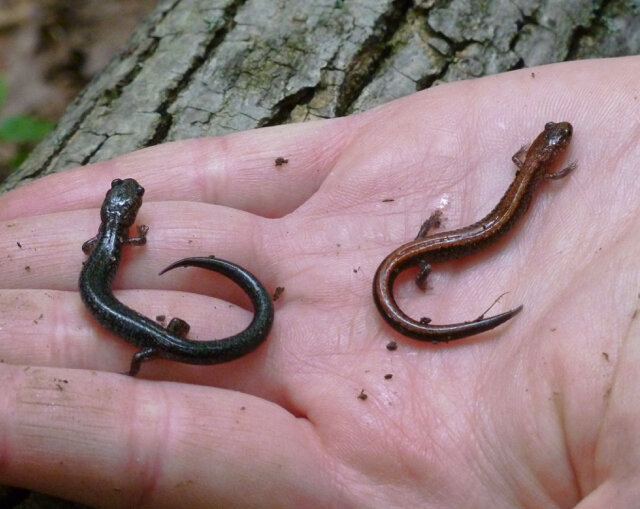
\includegraphics[width=0.5\linewidth]{images/03_plciMorph} 

}

\caption{Unstriped (left) and striped color morphs of red-backed salamanders.}\label{fig:c3f1}
\end{figure}

Let's start by examining an example dataset. A \textbf{dataset} is simply a collection of data, often multiple types. This example dataset is about a phenomenon in wildlife biology called tail autotomy, which refers to the ability of organisms like salamanders and lizards to drop their tail when attacked by a predator. The tail continues to move after it's severed, which is thought to be an adaptation to avoid being eaten. In this case, tail autotomy data was collected for red-backed salamanders (\emph{Plethodon cinereus}), including two different color morphs (striped and unstriped) that are known differ in various behavioral and physiological traits (Figure \ref{fig:c3f1}). The dataset was collected by a former undergraduate student, \href{https://surgery.arizona.edu/person/banan-wael-otaibi-md}{Dr.~Banan Otaibi}, now a surgical resident at the University of Arizona. Dr.~Otaibi's research question was focused on whether tail autotomy behavior differs between color morphs.

\label{tab:c3t1}Dataset on tail autotomy in red-backed salamanders.

individual

morph

tail.sec

tail.vel

mass.g

length.cm

easting

northing

16O300

striped

110

3.0

0.8

3.9

350827

4699989

16O301

striped

160

2.3

0.7

4.0

350827

4699989

16O302

striped

250

2.8

0.9

3.9

350831

4699988

16O303

striped

360

3.3

1.0

4.0

350831

4699988

16O304

striped

220

4.6

0.6

3.4

350831

4699988

16O306

striped

120

3.0

0.6

3.3

352128

4702166

16O308

striped

310

3.5

1.2

4.2

352121

4702172

16O309

striped

220

2.6

0.8

3.7

352122

4702174

16O310

striped

360

2.4

0.7

3.6

352116

4702169

16O311

striped

410

2.6

0.9

3.8

352119

4702170

16O312

striped

190

2.2

1.0

3.8

352110

4702167

16O314

striped

460

2.9

0.8

3.5

352089

4702122

16O315

striped

420

2.2

0.5

3.4

352090

4702135

16O316

striped

440

4.0

0.6

3.3

352088

4702129

16O317

striped

400

3.4

0.9

4.0

352071

4702177

17O300

striped

180

3.5

1.1

4.4

351010

4700176

17O302

striped

270

3.8

0.5

3.2

350989

4700122

17O303

striped

50

1.7

0.6

3.6

350962

4700106

17O304

striped

340

3.2

0.8

4.0

350946

4700091

17O305

striped

300

3.2

1.0

4.1

350939

4700088

16O305

unstriped

10

0.5

0.4

3.1

352130

4702168

16O307

unstriped

0

0.0

0.9

3.6

352119

4702157

16O313

unstriped

20

0.8

0.4

2.9

352090

4702123

16O318

unstriped

10

1.1

0.6

3.3

352075

4702046

17O301

unstriped

70

1.9

0.5

3.3

350990

4700114

17O306

unstriped

70

2.0

0.3

2.8

350910

4700059

17O307

unstriped

10

0.9

0.8

4.2

350910

4700057

17O308

unstriped

30

1.7

0.8

4.0

350887

4700003

17O309

unstriped

50

1.2

1.0

3.9

350889

4699994

17O310

unstriped

50

1.3

0.6

3.4

350893

4700009

17O311

unstriped

0

0.0

0.5

3.5

350855

4699997

17O312

unstriped

0

0.0

0.8

4.0

350871

4700003

17O313

unstriped

50

1.6

0.8

3.9

350838

4700072

17O314

unstriped

20

0.6

0.4

3.0

350982

4700003

17O315

unstriped

20

0.6

0.6

3.4

350957

4699969

17O316

unstriped

50

1.8

0.5

3.5

350795

4699993

17O317

unstriped

50

2.0

0.6

3.6

350789

4700005

17O318

unstriped

40

0.8

0.5

3.4

350811

4700018

17O319

unstriped

50

1.9

0.4

3.1

350806

4700007

17O320

unstriped

80

1.4

0.5

3.3

350812

4700030

\subsection{Variables and observations}\label{variables-and-observations}

The first thing to notice is that the dataset is organized as a table, where each column represents a unique \textbf{variable} and each row represents a unique \textbf{observation} for each observation. A variable is simply a particular type of data, where the observations or measurements can vary. There are eight variables and 40 observations for each variable in the example dataset. Each variable has a unique name. The number of observations for a variable is called the \textbf{sample size}, which is denoted \(n\) or \(N\).

Data are often organized in this tabular format, whether it is in spreadsheet software like Google Sheets or Microsoft Excel, or as we'll see later in this chapter, in statistical software like R. Other names for this tabular format include a \textbf{data matrix} or \textbf{dataframe}, but they all have the common structure of variables in columns and observations in rows. The observations are also referenced under different names, such as measurements, cases, or individuals.

\subsection{Types of varaibles}\label{types-of-varaibles}

Variables can be distinguished between two general types, each with subtypes:

\begin{enumerate}
\def\labelenumi{\arabic{enumi}.}
\item
  \textbf{\emph{Quantitative variables}} Quantitative variables are defined by the observations taking on a range of numeric values. In fact, a synonymous name for a quantitative variable is a \textbf{numeric}. Some quantitative variables have observations that only take on \textbf{discrete} values, such as the number of amino acids composing a protein. In the example dataset, \texttt{tail.sec}, the number of seconds an automized tail moved, is measured as a discrete variable. Other variables are are measured on a \textbf{continuous} scale down to any number of decimal places. For example, mass (\texttt{mass.g}), length (\texttt{length.cm}), and tail velocity (\texttt{tail.vel}, the maximum observed nnumber of tail osciltions) are continuous variables.

  Sometimes quantitative variables can be measured on a discrete or a contiuous scale. For example, you might notice I said \texttt{tail.sec} is \textbf{measured} as a discrete variable, because the observations are integers. But seconds could of course be measured on a continuous scale (e.g., 3.4 seconds).
\item
  \textbf{\emph{Qualitative variables}} Qualitative variables are defined by the observations being classified into different categories. Indeed, qualitative variables are often referred to as \textbf{categorical}, or \textbf{factor} variables. Like quantitative variables, there are different types of qualitative variables. These subcategories reflect whether or not the categories of a variable have an inherent order. When the categories do not have an order, the variable is called \textbf{nominal}. In the example dataset, color morph (\texttt{morph}) is a nominal variable because the categories, striped and unstriped, do not have an order. Other categorical variables have order, such as the life stages of ticks (larva, nymph, adult). Life stage is an \textbf{ordinal} variable, reflecting the ordering in which individuals move through the different life stages.

  Qualitative variables can also be differentiated by the number of categories making up the variable. Specifically, variables with only two categories are called \textbf{binary} variables. Salamander color morph is a good example of a binary variable because color morph can either be striped or unstriped.

  Sometimes it's hard to classify a variable definitively. For example, consider \texttt{individual} in the example dataset. This is simply an alphanumeric code assigned as a unique id for each individual in the dataset. The last few digits of the code are indeed ordered, but the order isn't meaningful.
\end{enumerate}

\subsection{Relationships between variables}\label{relationships-between-variables}

When we ask research questions about causality, we can generally define two types of variables: the variable (or variables - indeed, many processes are not monocausal) inducing a causal effect, and the variable receiving the effect. In the scientific literature, people refer to these different types of variables with different names, so it's a good idea to become familiar with some of the most common terms.

A variable inducing a causal effect is often referred to as an \textbf{explanatory variable}. For example, we might conduct a study on how different types of medication affect blood pressure. In this case, medication type is the explanatory variable. Another common term people use for an explanatory variable is the \textbf{exposure variable}. Here the idea is that the type of medication an individual is exposed to has a causal effect on blood pressures.

The variable receiving causal effects is often referred to the \textbf{response variable}. In the example on medication and blood pressure, blood pressure is the response variable. Another common term for a response variable is an \textbf{outcome variable}.

I will generally use these terms throughout the book, but note these are not the only terms you'll see in the literature. For example, some people refer to explanatory variables as \textbf{independent variables} and response variables as \textbf{dependent variables}. I'm going to avoid using those terms as I tend to think they're confusing because sometimes there are relationships among explanatory variables (i.e., they are \emph{not} independent).

Also note that research questions about prediction are inherently interested in relationships between variables, with the caveat that those relaitonships may not be causal. The research question on tail autotomy is a good example of that. In that case, color morph is the explanatory variable, and we measured two different response variables, total tail movement time (\texttt{tail.sec}) and initial tail velocity (\texttt{tail.vel}). Color morph may well predict tail autotomy, but that relationship may not be causal. Perhaps there's a common genetic variant that contributes to both color morph and the degree of tail autotomy via physiological pathways. We'll explore examples like this in more detail in the next chapter.

\subsection{Variable naming conventions and metadata}\label{variable-naming-conventions-and-metadata}

It's good practice to use a consistent naming style for your variables. Notice that each of the variables in the example database are made of all lower case letters. Some variable names are made up of multiple words or abbreviations, and in the example dataset those components are separated by a period (\texttt{tail.vel}). Those variables with multiple components do not have spaces because spaces are not handled well in statistical software, particularly code-based software (like R). Other conventions to separate components of a variable name work just fine; for example one could separate different components by an underscore (\texttt{tail\_vel}), or by capitalizing the first letter of a new component (\texttt{tailVel}). The most important thing is to be consistent in your approach.

It's also a good idea to get in the habit of generating metadata to go along with your dataset. Metadata is a description of the dataset, including defintiions of variables, their units of measure, and more. Here's some metadata describing the variables in the example dataset:

\begin{table}
\centering
\caption{\label{tab:c3t2}Variable descriptions for a study of the relationship between tail autotomy behavior and color morphology in red-backed salamanders.}
\centering
\begin{tabular}[t]{l|l}
\hline
Variable & Description\\
\hline
individual & Unique identification code for each individual salamander.\\
\hline
morph & Color morph (striped or unstriped) for each salamander.\\
\hline
tail.sec & Total tail movement time (seconds).\\
\hline
tail.vel & Initial tail movement velocity, measured as the maximum observed oscillations per second.\\
\hline
mass.g & Mass in grams\\
\hline
length.cm & Snout-vent-length in cm\\
\hline
easting & Longitudinal geographic coordinate in UTM zone 18 projection (meters).\\
\hline
northing & Latitudinal geographic coordinate in UTM zone 18 projection (meters).\\
\hline
\end{tabular}
\end{table}

\section{Introduction to R}\label{introduction-to-r}

Statistical software is a means to an end. Ultimately our goal is to do good science, and to do that, we must collect and analyze data. In this book, I use the statistical platform R to conduct analyses and create graphical outputs of data. You can find many types of software to perform basic data analyses commonly taught as part of an introductory statistics course. Some are free, and some are not. Some have a graphical user interface where you can point and click to select analyses (e.g., SPSS, JMP), some are spreadsheet-based (e.g., Excel, Google Sheets), and others are code-based, requiring the user to write their own computer code scripts to perform analyses. R is 100\% free, code-based, and widely used in science. In this appendix, I introduce you to the basic data processing skills needed to use R. This material is really intended for those who have no experience using R before. The idea is to introduce some basic skills that will get you up to speed so that you can follow the code and explanations in the book. If you have previously learned basic data processing in R, you can probably skip this material.

\subsection{Installing R and RStudio}\label{installing-r-and-rstudio}

Whereas R is a code-based engine for data processing and analysis, RStudio is an interface that makes it easy to work in R. One of the main advantages of using RStudio to access R is that it is easy to visualize, execute, and save scripts of R code. So while all of the code in this appendix and throughout the book can be executed directly in R, I strongly encourage working with R via RStudio. Like R, RStudio is free.

If you want to install R and RStudio on your own computer, the first thing you should do is download and install R from \url{https://www.r-project.org/}. Click the ``CRAN'' or ``download R'' link, and then choose any mirror to access a download link for your platform (e.g., macOS, Windows, Linux). Once you have installed R, head over to from \url{https://posit.co/download/rstudio-desktop/} and click the the link to Install RStudio, then follow the instructions.

There are also ways of using R and RStudio via cloud-based platforms. Fore example, many universities have invested in \href{https://posit.cloud}{Posit Cloud} for this functionality. With Posit Cloud, you don't need to install R or RStudio to your hard drive, and R code can be easily shared with others. Although it is often handy to have R and RStudio directly on your hard drive, many courses in research design and statistics access R and RStudio via Posit Cloud, so I wanted to mention it here.

\subsection{The RStudio Interface}\label{the-rstudio-interface}

When initially opened, the RStudio interface includes three sections (Figure \ref{fig:c3c1}). The console pane is on the left side, which is where you work with the R environment by typing in or executing code. For numerical data processing, output of your code will generally be displayed in the console (though not always automatically). Graphical output will be displayed in the output pane on the bottom right when viewing the Plots tab. Other tabs in the bottom right allow one to navigate to files on your hard drive, examine help documents, and more. The section at the top right is the Environment pane, which shows the objects that you have loaded in R. We'll dig in first on how to compose and execute code in the R Console.

\begin{figure}

{\centering 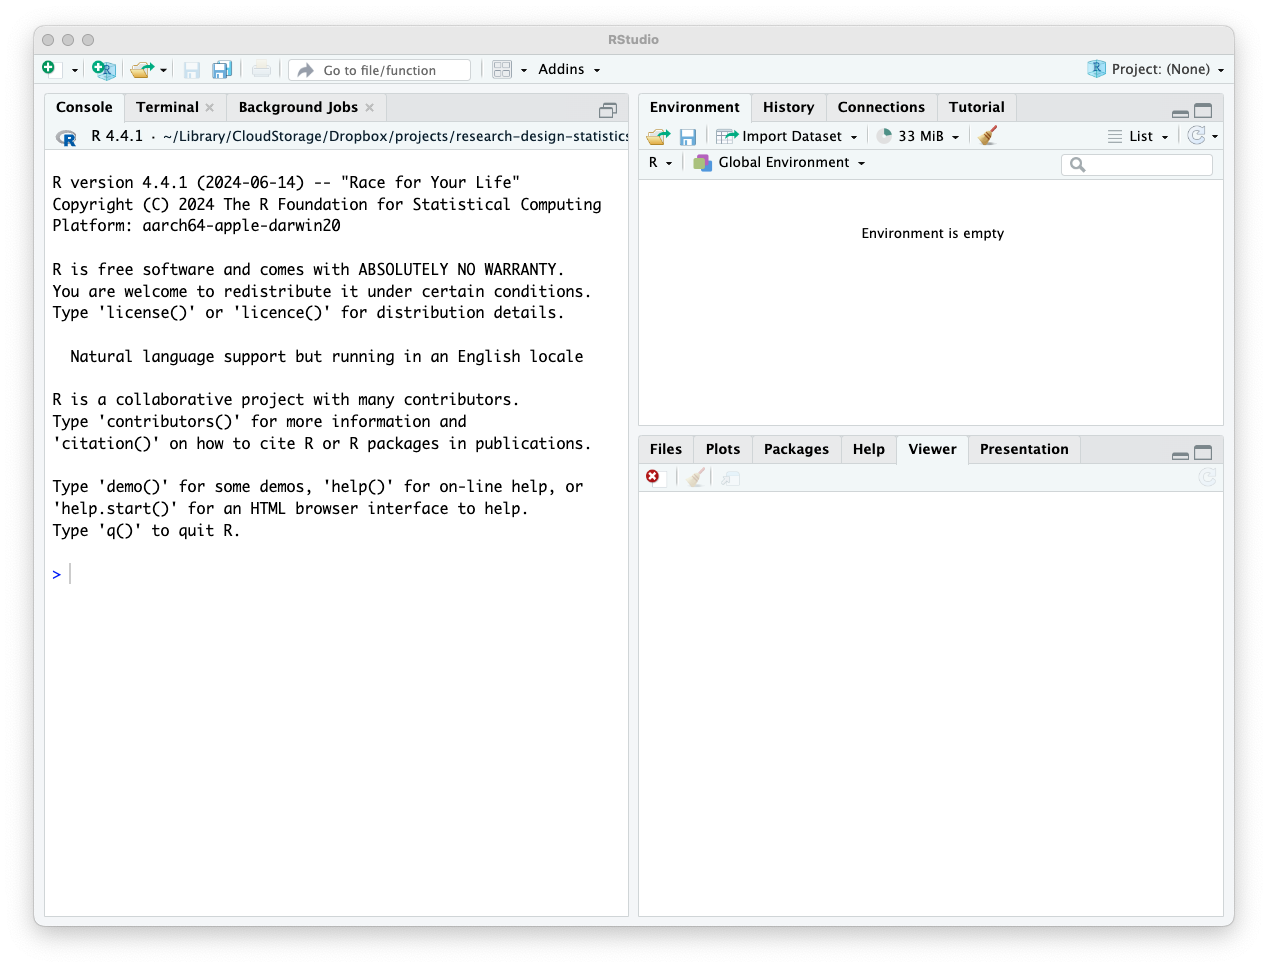
\includegraphics[width=0.8\linewidth]{images/03_rStudio} 

}

\caption{RStudio interface showing the R console (left), working environment (top right), and output (bottom right) panes.}\label{fig:c3c1}
\end{figure}

\subsection{Basic data manipulation in R}\label{basic-data-manipulation-in-r}

\subsubsection{R as a Calculator}\label{r-as-a-calculator}

Let's start simple by using R as a calculator. When you start R, you'll see some background on the version of R you're using and some related information. Below all that you'll see a greater than sign (\texttt{\textgreater{}}). This is the command prompt, and it's where you will type in code that you want to execute. For example, you can do a basic arithmetic such as 2+2 by simply typing in 2+2 and pressing enter.

\begin{Shaded}
\begin{Highlighting}[]
\DecValTok{2}\SpecialCharTok{+}\DecValTok{2}
\end{Highlighting}
\end{Shaded}

\begin{verbatim}
## [1] 4
\end{verbatim}

In the book, I've highlighted R code and like that above in a gray block. Every time I include a chunk of R code, you'll see the command prompt and code to be executed in gray, followed by the output (also in gray), which is the result of the code. So for a simple computation of 2 + 2, you see the command prompt, the 2 + 2 code, and then the output of 4. R prints a number next to the output, here being {[}1{]} for the first line of output.

If you want to include notes in your R code that are not executed as code, all you have to do is add a hash sign (\#) before the text of your note, like this:

\begin{Shaded}
\begin{Highlighting}[]
\DecValTok{2}\SpecialCharTok{+}\DecValTok{2} \CommentTok{\#simple addition}
\end{Highlighting}
\end{Shaded}

\begin{verbatim}
## [1] 4
\end{verbatim}

Here I've added the note \texttt{"simple\ addition"}, which is ignored by R because I included a number side before the text ``simple addition''. See what happens if you don't include the number sign to specify your note:

\begin{Shaded}
\begin{Highlighting}[]
\DecValTok{2}\SpecialCharTok{+}\DecValTok{2}\NormalTok{ simple addition}
\end{Highlighting}
\end{Shaded}

\begin{verbatim}
## Error: <text>:1:5: unexpected symbol
## 1: 2+2 simple
##         ^
\end{verbatim}

The dreaded red warning text! When output is highlighted in red, that's usually R's way of telling you there's a problem. Here the problem is that R doesn't know what to do with the word ``simple''. There's no number sign signifying ``simple addition'' as a note that should be ignored, so R assumes it's part of your code. Also note that R doesn't even get to ``addition'', it stops executing your code at ``simple'' because it doesn't know how to proceed.

OK, so that's some background on how to execute a simple arithmetic function and include a note. Now go ahead and perform some basic arithmetic computations:

\begin{Shaded}
\begin{Highlighting}[]
\DecValTok{4}\SpecialCharTok{*}\DecValTok{3} \CommentTok{\#simple multiplication}
\end{Highlighting}
\end{Shaded}

\begin{verbatim}
## [1] 12
\end{verbatim}

\begin{Shaded}
\begin{Highlighting}[]
\DecValTok{20}\SpecialCharTok{/}\DecValTok{4} \CommentTok{\#simple division}
\end{Highlighting}
\end{Shaded}

\begin{verbatim}
## [1] 5
\end{verbatim}

\begin{Shaded}
\begin{Highlighting}[]
\FunctionTok{log}\NormalTok{(}\DecValTok{42}\NormalTok{) }\CommentTok{\#the natural log function}
\end{Highlighting}
\end{Shaded}

\begin{verbatim}
## [1] 3.73767
\end{verbatim}

\begin{Shaded}
\begin{Highlighting}[]
\FunctionTok{sqrt}\NormalTok{(}\DecValTok{4}\NormalTok{) }\CommentTok{\#the square root function}
\end{Highlighting}
\end{Shaded}

\begin{verbatim}
## [1] 2
\end{verbatim}

\begin{Shaded}
\begin{Highlighting}[]
\DecValTok{4}\SpecialCharTok{\^{}}\DecValTok{3} \CommentTok{\#raising 4 to the third power}
\end{Highlighting}
\end{Shaded}

\begin{verbatim}
## [1] 64
\end{verbatim}

We're on our way! In the preceding examples, you can see that some text in R is actually meaningful and does not lead to an error. For example, \texttt{log(42)} computes the natural log of 42, and \texttt{sqrt(4)} computes the square root of four. In this case, \texttt{log} and \texttt{sqr}'' are built-in functions in R. More on that soon!

\subsubsection{Objects}\label{objects}

As you can see, it's pretty straightforward to use R as a calculator, but R can do much more. One of the most useful aspects of R is storing data as objects. As a very simple example, suppose we want to assign a value of 4 to a variable that we'll call \texttt{x}:

\begin{Shaded}
\begin{Highlighting}[]
\NormalTok{x }\OtherTok{\textless{}{-}} \DecValTok{4}
\end{Highlighting}
\end{Shaded}

Here we have defined \texttt{x} as 4 with the left arrow, which is a less than sign followed by a dash. The arrow indicates the flow of information, with x on the left being defined as 4. There's nothing special about ``x'' here. For example, I could have defined ``y'' as 4:

\begin{Shaded}
\begin{Highlighting}[]
\NormalTok{y }\OtherTok{\textless{}{-}} \DecValTok{4}
\end{Highlighting}
\end{Shaded}

Or, you can define the object \texttt{Taylor.Swift} as 4:

\begin{Shaded}
\begin{Highlighting}[]
\NormalTok{Taylor.Swift }\OtherTok{\textless{}{-}} \DecValTok{4}
\end{Highlighting}
\end{Shaded}

Note that I didn't include a space between ``Taylor'' and ``Swift''. Try it with a space and see what happens:

\begin{Shaded}
\begin{Highlighting}[]
\NormalTok{Taylor Swift }\OtherTok{\textless{}{-}} \DecValTok{4}
\end{Highlighting}
\end{Shaded}

\begin{verbatim}
## Error: <text>:1:8: unexpected symbol
## 1: Taylor Swift
##            ^
\end{verbatim}

No good. R doesn't like spaces, so when I define objects that involve more than one word, I usually either include a period or underline between them, or I don't include any characters between them but distinguish components of a variable name by capitalization.

\begin{Shaded}
\begin{Highlighting}[]
\NormalTok{Taylor.Swift }\OtherTok{\textless{}{-}} \DecValTok{4}
\NormalTok{Taylor\_Swift }\OtherTok{\textless{}{-}} \DecValTok{4}
\NormalTok{TaylorSwift }\OtherTok{\textless{}{-}} \DecValTok{4}
\NormalTok{taylorSwift }\OtherTok{\textless{}{-}} \DecValTok{4}
\end{Highlighting}
\end{Shaded}

Notice that R is case sensitive! The objects \texttt{TaylorSwift} and \texttt{taylorSwift} are unique!

OK, great. So I've defined a whole bunch of objects as the value 4. Wait. How do I know each of these objects is 4? Well, type the object name into the R prompt and execute it, and you should see the result is 4:

\begin{Shaded}
\begin{Highlighting}[]
\NormalTok{x}
\end{Highlighting}
\end{Shaded}

\begin{verbatim}
## [1] 4
\end{verbatim}

\begin{Shaded}
\begin{Highlighting}[]
\NormalTok{Taylor.Swift}
\end{Highlighting}
\end{Shaded}

\begin{verbatim}
## [1] 4
\end{verbatim}

Cool! So R will store numeric values - data - symbolically. Quick note: R is case-sensitive. See what happens when you don't capitalize the T and S in \texttt{Taylor.Swift}:

\begin{Shaded}
\begin{Highlighting}[]
\NormalTok{taylor.swift}
\end{Highlighting}
\end{Shaded}

\begin{verbatim}
## Error in eval(expr, envir, enclos): object 'taylor.swift' not found
\end{verbatim}

The red text of death. Bummer. This is going to be a major source of frustration as you develop your coding skills. The smallest errors, like a lower-case character when it should be upper-case, will cause your code to fail. If you're hoping to work on your attention to detail, this is going to be a good way to do that!

When we define objects, we can start to use them in functions. For example, what's the square root of \texttt{Taylor.Swift}?

\begin{Shaded}
\begin{Highlighting}[]
\FunctionTok{sqrt}\NormalTok{(Taylor.Swift)}
\end{Highlighting}
\end{Shaded}

\begin{verbatim}
## [1] 2
\end{verbatim}

Clearly it's 2, because \texttt{Taylor.Swift} is 4, and the square root of 4 is 2. How about \texttt{x\ +\ y}?

\begin{Shaded}
\begin{Highlighting}[]
\NormalTok{x }\SpecialCharTok{+}\NormalTok{ y}
\end{Highlighting}
\end{Shaded}

\begin{verbatim}
## [1] 8
\end{verbatim}

Right on - \texttt{x} and \texttt{y} were both defined as 4, so \texttt{x\ +\ y} is 8. Note that we can define these output of these arithmetic functions as new objects:

\begin{Shaded}
\begin{Highlighting}[]
\NormalTok{z }\OtherTok{\textless{}{-}}\NormalTok{ x }\SpecialCharTok{+}\NormalTok{ y}
\NormalTok{z}
\end{Highlighting}
\end{Shaded}

\begin{verbatim}
## [1] 8
\end{verbatim}

Here we defined ``z'' as \texttt{x\ +\ y}, so \texttt{z} is 8. Note that objects can be used to pretty much any degree of complexity:

\begin{Shaded}
\begin{Highlighting}[]
\NormalTok{z}\SpecialCharTok{**}\NormalTok{(x}\SpecialCharTok{+}\NormalTok{y)}\SpecialCharTok{/}\NormalTok{(Taylor.Swift }\SpecialCharTok{{-}}\NormalTok{ x}\SpecialCharTok{**}\NormalTok{y}\SpecialCharTok{*}\NormalTok{z)}
\end{Highlighting}
\end{Shaded}

\begin{verbatim}
## [1] -8208.031
\end{verbatim}

Finally, objects don't have to be numbers. There are different types of objects in R. All of the objects we just defined are called numeric, because they are just numbers. We can also define objects as characters, which are simply strings of text and defined by quotation marks:

\begin{Shaded}
\begin{Highlighting}[]
\SpecialCharTok{\textgreater{}} \DocumentationTok{\#\# Character objects have quotation marks}
\ErrorTok{\textgreater{}}\NormalTok{ singer }\OtherTok{\textless{}{-}} \StringTok{"Taylor Swift"}
\SpecialCharTok{\textgreater{}}\NormalTok{ singer}
\NormalTok{[}\DecValTok{1}\NormalTok{] }\StringTok{"Taylor Swift"}
\end{Highlighting}
\end{Shaded}

Another type of object that we'll encounter a lot in statistics are factor variables, which are categorical variables. I will describe those later.

\subsubsection{Functions}\label{functions}

R has built-in functions that allow you to quickly perform calculations. We've already seen this, such as when we quantified the square root of 4 with the \texttt{sqrt} function. Remember that functions are usually called in R by specifying the name of the function followed by round brackets that enclose the arguments of the function:

\begin{Shaded}
\begin{Highlighting}[]
\SpecialCharTok{\textgreater{}} \FunctionTok{sqrt}\NormalTok{(}\DecValTok{4}\NormalTok{)}
\NormalTok{[}\DecValTok{1}\NormalTok{] }\DecValTok{2}
\end{Highlighting}
\end{Shaded}

The \texttt{sqrt} function is very simple in that it has a single argument, which is the numerical value for which you want to quantify the square root. Other functions have multiple arguments. For example, suppose you want to round the value of 3.147 to a single decimal place. You can use R's built-in \texttt{round} function to do that, which has two arguments. The first argument is the value \texttt{x} you want to round, and the second argument is the number of digits to round to. When you apply a function with multiple arguments, the arguments are separated by a comma:

\begin{Shaded}
\begin{Highlighting}[]
\SpecialCharTok{\textgreater{}} \FunctionTok{round}\NormalTok{(}\AttributeTok{x =} \FloatTok{3.147}\NormalTok{, }\AttributeTok{digits =} \DecValTok{1}\NormalTok{)}
\NormalTok{[}\DecValTok{1}\NormalTok{] }\FloatTok{3.1}
\end{Highlighting}
\end{Shaded}

How did I know which arguments are included in the \texttt{round} function? Built-in functions have supporting documentation that you can read to learn about the function and its arguments. To read the documentation, simply add a question mark in front of the function name, and execute that code:

\begin{Shaded}
\begin{Highlighting}[]
\NormalTok{?round}
\end{Highlighting}
\end{Shaded}

When you execute the code, the bottom right panel in RStudio will show you the ``Help'' document for the round function. You'll see an ``Arguments'' section, and there you'll see that the round function has two arguments (Figure \ref{fig:c3f3}.

\begin{figure}

{\centering 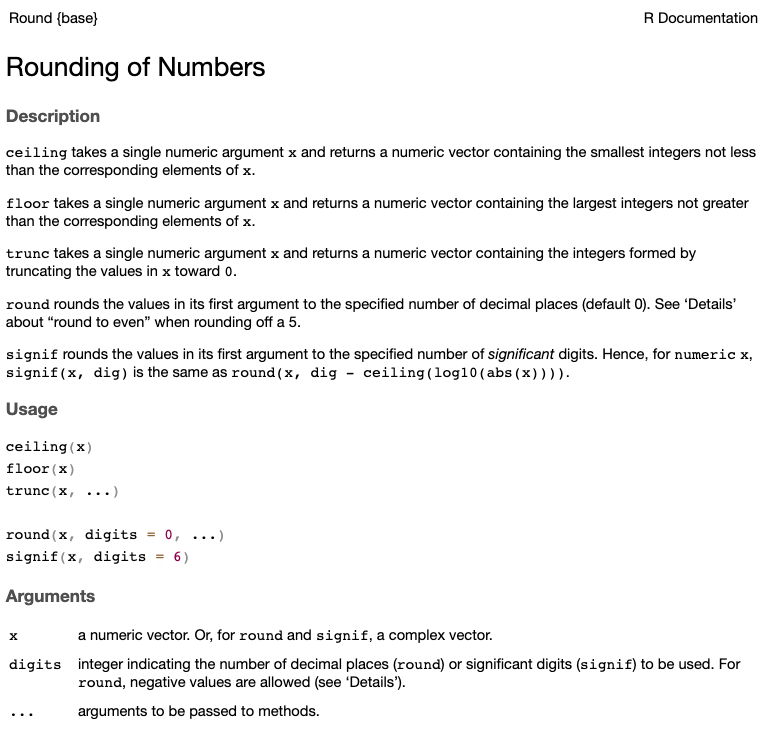
\includegraphics[width=0.8\linewidth]{images/03_documentation} 

}

\caption{Documentation for the round function.}\label{fig:c3f3}
\end{figure}

So we see here that the round function requires a numerical value ``x' to round and the number of''digits'' to round. When you execute code with a function, you can go ahead and use the name of each argument and then specify the value of the argument following an equal sign, like I did above. If you are naming the arguments, the order in which you present the arguments does not matter:

\begin{Shaded}
\begin{Highlighting}[]
\SpecialCharTok{\textgreater{}} \FunctionTok{round}\NormalTok{(}\AttributeTok{x =} \FloatTok{3.147}\NormalTok{, }\AttributeTok{digits =} \DecValTok{1}\NormalTok{)}
\NormalTok{[}\DecValTok{1}\NormalTok{] }\FloatTok{3.1}
\SpecialCharTok{\textgreater{}} \FunctionTok{round}\NormalTok{(}\AttributeTok{digits =} \DecValTok{1}\NormalTok{, }\AttributeTok{x =} \FloatTok{3.147}\NormalTok{)}
\NormalTok{[}\DecValTok{1}\NormalTok{] }\FloatTok{3.1}
\end{Highlighting}
\end{Shaded}

You don't have to name the arguments when executing a function, but there's a catch. When you apply a function and specify the value of the necessary arguments, you have to specify the arguments in the order in which the function expects (x and then digits):

\begin{Shaded}
\begin{Highlighting}[]
\FunctionTok{round}\NormalTok{(}\FloatTok{3.147}\NormalTok{, }\DecValTok{1}\NormalTok{)}
\end{Highlighting}
\end{Shaded}

\begin{verbatim}
## [1] 3.1
\end{verbatim}

If you use the reverse order, you get a different answer:

\begin{Shaded}
\begin{Highlighting}[]
\FunctionTok{round}\NormalTok{(}\DecValTok{1}\NormalTok{, }\FloatTok{3.147}\NormalTok{)}
\end{Highlighting}
\end{Shaded}

\begin{verbatim}
## [1] 1
\end{verbatim}

Note that arguments for a function often have default values. For example, the \texttt{digits} argument in the \texttt{round} function defaults to 0 if not specified, meaning that \texttt{round(3.147)} will round 3.147 to 0 decimal places. The default values can be found in the documentation under the Usage section.

\begin{Shaded}
\begin{Highlighting}[]
\FunctionTok{round}\NormalTok{(}\FloatTok{3.147}\NormalTok{)}
\end{Highlighting}
\end{Shaded}

\begin{verbatim}
## [1] 3
\end{verbatim}

There are many, many functions in R. For example, the function \texttt{class} makes R show what type of object you are dealing with:

\begin{Shaded}
\begin{Highlighting}[]
\SpecialCharTok{\textgreater{}} \FunctionTok{class}\NormalTok{(y)}
\NormalTok{[}\DecValTok{1}\NormalTok{] }\StringTok{"numeric"}
\SpecialCharTok{\textgreater{}} 
\ErrorTok{\textgreater{}} \FunctionTok{class}\NormalTok{(singer)}
\NormalTok{[}\DecValTok{1}\NormalTok{] }\StringTok{"character"}
\end{Highlighting}
\end{Shaded}

\subsubsection{Vectors}\label{vectors}

We know that datasets are made up of one or more variables, each with multiple observations. In R, we can store variables with multiple observations as \textbf{vectors}. For example, suppose we have data on body temperature for five individuals of different ages:

\begin{table}[H]
\centering\centering
\begin{tabular}{r|r}
\hline
\textbf{Age} & \textbf{Temperature (Celcius)}\\
\hline
22 & 98.2\\
\hline
28 & 99.1\\
\hline
34 & 99.3\\
\hline
43 & 98.4\\
\hline
50 & 98.9\\
\hline
\end{tabular}
\end{table}

We can use the concatenate function, \texttt{c}, to create vector for age and temperature:

\begin{Shaded}
\begin{Highlighting}[]
\SpecialCharTok{\textgreater{}} 
\ErrorTok{\textgreater{}} \CommentTok{\# The c() function combines individual values into a single vector}
\ErrorTok{\textgreater{}}\NormalTok{ age }\OtherTok{\textless{}{-}} \FunctionTok{c}\NormalTok{(}\DecValTok{22}\NormalTok{, }\DecValTok{28}\NormalTok{, }\DecValTok{34}\NormalTok{, }\DecValTok{43}\NormalTok{, }\DecValTok{50}\NormalTok{)}
\SpecialCharTok{\textgreater{}}\NormalTok{ age}
\NormalTok{[}\DecValTok{1}\NormalTok{] }\DecValTok{22} \DecValTok{28} \DecValTok{34} \DecValTok{43} \DecValTok{50}
\SpecialCharTok{\textgreater{}} 
\ErrorTok{\textgreater{}} \DocumentationTok{\#\# and now a vector for temperature}
\ErrorTok{\textgreater{}}\NormalTok{ temp }\OtherTok{\textless{}{-}} \FunctionTok{c}\NormalTok{(}\FloatTok{98.2}\NormalTok{, }\FloatTok{99.1}\NormalTok{, }\FloatTok{99.3}\NormalTok{, }\FloatTok{98.4}\NormalTok{, }\FloatTok{98.9}\NormalTok{)}
\SpecialCharTok{\textgreater{}}\NormalTok{ temp}
\NormalTok{[}\DecValTok{1}\NormalTok{] }\FloatTok{98.2} \FloatTok{99.1} \FloatTok{99.3} \FloatTok{98.4} \FloatTok{98.9}
\end{Highlighting}
\end{Shaded}

We can ask R to show us all the values of a vector by simply calling the name of the object, as I've done above. We can also ask R to report particular observations of a vector by using square brackets. For example, to have R report the fifth observation of the temperature vector:

\begin{Shaded}
\begin{Highlighting}[]
\SpecialCharTok{\textgreater{}}\NormalTok{ temp[}\DecValTok{5}\NormalTok{]}
\NormalTok{[}\DecValTok{1}\NormalTok{] }\FloatTok{98.9}
\end{Highlighting}
\end{Shaded}

Note that the temp vector has five observations. What happens if we ask for the sixth observation?

\begin{Shaded}
\begin{Highlighting}[]
\NormalTok{temp[}\DecValTok{6}\NormalTok{]}
\end{Highlighting}
\end{Shaded}

\begin{verbatim}
## [1] NA
\end{verbatim}

Here R reports ``NA'', which means ``not available''. This is simply R's way of telling you that the value you asked for doesn't exist.

If you want to view multiple observations for a vector, you can specify multiple observations with the concatenate function, or you can use a colon to show consecutive observations:

\begin{Shaded}
\begin{Highlighting}[]
\SpecialCharTok{\textgreater{}} 
\ErrorTok{\textgreater{}} \DocumentationTok{\#\# Show the 3rd and 5th observation:}
\ErrorTok{\textgreater{}}\NormalTok{ temp[}\FunctionTok{c}\NormalTok{(}\DecValTok{3}\NormalTok{,}\DecValTok{5}\NormalTok{)]}
\NormalTok{[}\DecValTok{1}\NormalTok{] }\FloatTok{99.3} \FloatTok{98.9}
\SpecialCharTok{\textgreater{}} 
\ErrorTok{\textgreater{}} \DocumentationTok{\#\# Show the 3rd through the 5th observation:}
\ErrorTok{\textgreater{}}\NormalTok{ temp[}\DecValTok{3}\SpecialCharTok{:}\DecValTok{5}\NormalTok{]}
\NormalTok{[}\DecValTok{1}\NormalTok{] }\FloatTok{99.3} \FloatTok{98.4} \FloatTok{98.9}
\end{Highlighting}
\end{Shaded}

If you want to view observations while excluding particular observations, you can do that by adding a minus sign in front of the observation(s) you want to exclude:

\begin{Shaded}
\begin{Highlighting}[]
\SpecialCharTok{\textgreater{}} 
\ErrorTok{\textgreater{}} \DocumentationTok{\#\# Show all but the third observation:}
\ErrorTok{\textgreater{}}\NormalTok{ temp[}\SpecialCharTok{{-}}\DecValTok{3}\NormalTok{]}
\NormalTok{[}\DecValTok{1}\NormalTok{] }\FloatTok{98.2} \FloatTok{99.1} \FloatTok{98.4} \FloatTok{98.9}
\SpecialCharTok{\textgreater{}} 
\ErrorTok{\textgreater{}} \DocumentationTok{\#\# Show all but the third and fifth observation}
\ErrorTok{\textgreater{}}\NormalTok{ temp[}\SpecialCharTok{{-}}\FunctionTok{c}\NormalTok{(}\DecValTok{3}\NormalTok{,}\DecValTok{5}\NormalTok{)]}
\NormalTok{[}\DecValTok{1}\NormalTok{] }\FloatTok{98.2} \FloatTok{99.1} \FloatTok{98.4}
\end{Highlighting}
\end{Shaded}

We can easily apply arithmetic functions to vectors. For example, suppose I wanted to know how many degrees each individual's body temperature is above or below what's considered the ``normal'' value of 98.6 Celcius. Here I'll just ask R to subtract 98.6 from each value in \texttt{temp}, and then save that output as a new object called \texttt{temp.deviation}:

\begin{Shaded}
\begin{Highlighting}[]
\SpecialCharTok{\textgreater{}} 
\ErrorTok{\textgreater{}} 
\ErrorTok{\textgreater{}}\NormalTok{ temp.deviation }\OtherTok{\textless{}{-}}\NormalTok{ temp}\FloatTok{{-}98.6}
\SpecialCharTok{\textgreater{}} 
\ErrorTok{\textgreater{}}\NormalTok{ temp.deviation}
\NormalTok{[}\DecValTok{1}\NormalTok{] }\SpecialCharTok{{-}}\FloatTok{0.4}  \FloatTok{0.5}  \FloatTok{0.7} \SpecialCharTok{{-}}\FloatTok{0.2}  \FloatTok{0.3}
\end{Highlighting}
\end{Shaded}

Here we can see that the first individual's temperature is 0.4 degrees below normal, the second individual is 0.5 degrees above normal, and so forth.

\subsubsection{Matrices}\label{matrices}

Recall that we have body temperature data for individuals of different ages. So far we have created separate vectors for each variable, but each vector has the same structure (5 observations). Remember that datasets of multiple variables are usually organized in a tabular format, with columns representing different variables and rows representing the multiple observations of each variable. In R, we can combine vectors into a single data table called a \textbf{matrix}. Matrices are made of rows and columns, just like a spreadsheet, where the rows represent observations, and the columns represent different objects. Let's make a matrix for our age and temperature data using the \texttt{cbind} function, which combines objects into multiple columns. We'll save this new table and name it \texttt{patient.table}:

\begin{Shaded}
\begin{Highlighting}[]
\SpecialCharTok{\textgreater{}} 
\ErrorTok{\textgreater{}}\NormalTok{ patient.table }\OtherTok{\textless{}{-}} \FunctionTok{cbind}\NormalTok{(age, temp)}
\SpecialCharTok{\textgreater{}} 
\ErrorTok{\textgreater{}}\NormalTok{ patient.table}
\NormalTok{     age temp}
\NormalTok{[}\DecValTok{1}\NormalTok{,]  }\DecValTok{22} \FloatTok{98.2}
\NormalTok{[}\DecValTok{2}\NormalTok{,]  }\DecValTok{28} \FloatTok{99.1}
\NormalTok{[}\DecValTok{3}\NormalTok{,]  }\DecValTok{34} \FloatTok{99.3}
\NormalTok{[}\DecValTok{4}\NormalTok{,]  }\DecValTok{43} \FloatTok{98.4}
\NormalTok{[}\DecValTok{5}\NormalTok{,]  }\DecValTok{50} \FloatTok{98.9}
\end{Highlighting}
\end{Shaded}

We can use square brackets to access observations in a matrix, but now we have to consider that we have two dimensions of data: rows and columns. To extract observations from a matrix, we use a square bracket with row and column values separated by a comma. For example, let's say we want to view the age of the second individual. The second individual is in row 2, and age is the first column in our matrix:

\begin{Shaded}
\begin{Highlighting}[]
\SpecialCharTok{\textgreater{}} 
\ErrorTok{\textgreater{}} \DocumentationTok{\#\# show the age of the second individual}
\ErrorTok{\textgreater{}}\NormalTok{ patient.table[}\DecValTok{2}\NormalTok{,}\DecValTok{1}\NormalTok{]}
\NormalTok{age }
 \DecValTok{28} 
\end{Highlighting}
\end{Shaded}

What if we wanted to view the age AND temperature for the second individual. In this case, we can just leave the column value blank, which R interprets as requesting all the columns:

\begin{Shaded}
\begin{Highlighting}[]
\SpecialCharTok{\textgreater{}} 
\ErrorTok{\textgreater{}} \DocumentationTok{\#\# show all data for the second individual}
\ErrorTok{\textgreater{}}\NormalTok{ patient.table[}\DecValTok{2}\NormalTok{,]}
\NormalTok{ age temp }
\FloatTok{28.0} \FloatTok{99.1} 
\end{Highlighting}
\end{Shaded}

We can also view all the observations for a single variable. Let's say we want to view just the temperature data again. Here we will leave the row value blank but specify the second column for temperature:

\begin{Shaded}
\begin{Highlighting}[]
\SpecialCharTok{\textgreater{}} 
\ErrorTok{\textgreater{}} \DocumentationTok{\#\# show the temperature values}
\ErrorTok{\textgreater{}}\NormalTok{ patient.table[,}\DecValTok{2}\NormalTok{]}
\NormalTok{[}\DecValTok{1}\NormalTok{] }\FloatTok{98.2} \FloatTok{99.1} \FloatTok{99.3} \FloatTok{98.4} \FloatTok{98.9}
\end{Highlighting}
\end{Shaded}

What if we want to add more variables? Let's say we have the body mass index (BMI) for each individual and want to add it to the matrix. We could just create a vector \texttt{bmi}, and then combine it with the other two vectors, or combine it with the \texttt{patient.table} matrix. Either will produce the same output:'

\begin{Shaded}
\begin{Highlighting}[]
\SpecialCharTok{\textgreater{}} 
\ErrorTok{\textgreater{}} \DocumentationTok{\#\# create a bmi vector}
\ErrorTok{\textgreater{}}\NormalTok{ bmi }\OtherTok{\textless{}{-}} \FunctionTok{c}\NormalTok{(}\DecValTok{20}\NormalTok{, }\DecValTok{24}\NormalTok{, }\DecValTok{21}\NormalTok{, }\DecValTok{23}\NormalTok{, }\DecValTok{24}\NormalTok{)}
\SpecialCharTok{\textgreater{}} 
\ErrorTok{\textgreater{}} \DocumentationTok{\#\# combine each vector to create a table}
\ErrorTok{\textgreater{}}\NormalTok{ patient.table.new }\OtherTok{\textless{}{-}} \FunctionTok{cbind}\NormalTok{(age, temp, bmi)}
\SpecialCharTok{\textgreater{}} 
\ErrorTok{\textgreater{}} \DocumentationTok{\#\# or just combine the original table with the new bmi vector}
\ErrorTok{\textgreater{}}\NormalTok{ patient.table }\OtherTok{\textless{}{-}} \FunctionTok{cbind}\NormalTok{(patient.table, bmi)}
\SpecialCharTok{\textgreater{}} 
\ErrorTok{\textgreater{}}\NormalTok{ patient.table}
\NormalTok{     age temp bmi}
\NormalTok{[}\DecValTok{1}\NormalTok{,]  }\DecValTok{22} \FloatTok{98.2}  \DecValTok{20}
\NormalTok{[}\DecValTok{2}\NormalTok{,]  }\DecValTok{28} \FloatTok{99.1}  \DecValTok{24}
\NormalTok{[}\DecValTok{3}\NormalTok{,]  }\DecValTok{34} \FloatTok{99.3}  \DecValTok{21}
\NormalTok{[}\DecValTok{4}\NormalTok{,]  }\DecValTok{43} \FloatTok{98.4}  \DecValTok{23}
\NormalTok{[}\DecValTok{5}\NormalTok{,]  }\DecValTok{50} \FloatTok{98.9}  \DecValTok{24}
\end{Highlighting}
\end{Shaded}

Sometimes we don't have complete data for every variable. In R, remember that missing data are recorded as \texttt{NA} (``Not Available''). For example, suppose we have data on height (inches) for all but the third individual in our dataset. We would specify \texttt{NA} for that individual:

\begin{Shaded}
\begin{Highlighting}[]
\SpecialCharTok{\textgreater{}} 
\ErrorTok{\textgreater{}} \DocumentationTok{\#\# create a height vector}
\ErrorTok{\textgreater{}}\NormalTok{ height }\OtherTok{\textless{}{-}} \FunctionTok{c}\NormalTok{(}\DecValTok{65}\NormalTok{, }\DecValTok{71}\NormalTok{, }\ConstantTok{NA}\NormalTok{, }\DecValTok{68}\NormalTok{, }\DecValTok{66}\NormalTok{)}
\SpecialCharTok{\textgreater{}} 
\ErrorTok{\textgreater{}} \DocumentationTok{\#\# add to the matrix}
\ErrorTok{\textgreater{}}\NormalTok{ patient.table }\OtherTok{\textless{}{-}} \FunctionTok{cbind}\NormalTok{(patient.table, height)}
\SpecialCharTok{\textgreater{}} 
\ErrorTok{\textgreater{}}\NormalTok{ patient.table}
\NormalTok{     age temp bmi height}
\NormalTok{[}\DecValTok{1}\NormalTok{,]  }\DecValTok{22} \FloatTok{98.2}  \DecValTok{20}     \DecValTok{65}
\NormalTok{[}\DecValTok{2}\NormalTok{,]  }\DecValTok{28} \FloatTok{99.1}  \DecValTok{24}     \DecValTok{71}
\NormalTok{[}\DecValTok{3}\NormalTok{,]  }\DecValTok{34} \FloatTok{99.3}  \DecValTok{21}     \ConstantTok{NA}
\NormalTok{[}\DecValTok{4}\NormalTok{,]  }\DecValTok{43} \FloatTok{98.4}  \DecValTok{23}     \DecValTok{68}
\NormalTok{[}\DecValTok{5}\NormalTok{,]  }\DecValTok{50} \FloatTok{98.9}  \DecValTok{24}     \DecValTok{66}
\end{Highlighting}
\end{Shaded}

\subsubsection{Data types in R}\label{data-types-in-r}

Recall that we can generally differentiate variables by their type, either quantitative or qualitative. Each of the four variables we've created so far (\texttt{age}, \texttt{temp}, \texttt{bmi}, \texttt{height}) are quantitative. R defines variable types by their \textbf{class}, and you can ask R to return each object's classification with the \textbf{class} function;

\begin{Shaded}
\begin{Highlighting}[]
\SpecialCharTok{\textgreater{}} 
\ErrorTok{\textgreater{}} \FunctionTok{class}\NormalTok{(age)}
\NormalTok{[}\DecValTok{1}\NormalTok{] }\StringTok{"numeric"}
\SpecialCharTok{\textgreater{}} \FunctionTok{class}\NormalTok{(temp)}
\NormalTok{[}\DecValTok{1}\NormalTok{] }\StringTok{"numeric"}
\SpecialCharTok{\textgreater{}} \FunctionTok{class}\NormalTok{(bmi)}
\NormalTok{[}\DecValTok{1}\NormalTok{] }\StringTok{"numeric"}
\SpecialCharTok{\textgreater{}} \FunctionTok{class}\NormalTok{(height)}
\NormalTok{[}\DecValTok{1}\NormalTok{] }\StringTok{"numeric"}
\end{Highlighting}
\end{Shaded}

We can see R identifies each of these vectors as \textbf{numeric}, which is synonymous with quantitative. Qualitative variables in R are usually classified as \textbf{character} or \textbf{factor} variables. For example, let's create a nominal qualitative variable \textbf{sex}, defining each individual in our dataset as male or female:

\begin{Shaded}
\begin{Highlighting}[]
\DocumentationTok{\#\# create a character for sex}
\NormalTok{sex }\OtherTok{\textless{}{-}} \FunctionTok{c}\NormalTok{(}\StringTok{"female"}\NormalTok{, }\StringTok{"female"}\NormalTok{, }\StringTok{"male"}\NormalTok{, }\StringTok{"female"}\NormalTok{, }\StringTok{"male"}\NormalTok{)}
\FunctionTok{class}\NormalTok{(sex)}
\end{Highlighting}
\end{Shaded}

\begin{verbatim}
## [1] "character"
\end{verbatim}

Notice that \texttt{sex} is classified as a character because the observations consist of text rather than numbers. The other common way of defining and analyzing nominal variables in R is as a factor. We can change the object \texttt{sex} from a character to a factor variable by using the \texttt{as.factor} function:

\begin{Shaded}
\begin{Highlighting}[]
\DocumentationTok{\#\# create a character for sex}
\NormalTok{sex }\OtherTok{\textless{}{-}} \FunctionTok{as.factor}\NormalTok{(sex)}
\FunctionTok{class}\NormalTok{(sex)}
\end{Highlighting}
\end{Shaded}

\begin{verbatim}
## [1] "factor"
\end{verbatim}

When an object is stored as a factor, you can ask R to show you all the levels (i.e., categories) for the variable with the \texttt{levels} function:

\begin{Shaded}
\begin{Highlighting}[]
\FunctionTok{levels}\NormalTok{(sex)}
\end{Highlighting}
\end{Shaded}

\begin{verbatim}
## [1] "female" "male"
\end{verbatim}

Factor variables in R can also consist of levels that are numbers. For example, suppose that we assigned each individual in our dataset to one of three treatments, named ``1'', ``2'', and ``3''. When we initially define the treatment object, R will interpret the class as numeric, but we can change it to a factor:

\begin{Shaded}
\begin{Highlighting}[]
\DocumentationTok{\#\# create treatment variable with numeric codes}
\NormalTok{trt }\OtherTok{\textless{}{-}} \FunctionTok{c}\NormalTok{(}\DecValTok{1}\NormalTok{,}\DecValTok{2}\NormalTok{,}\DecValTok{3}\NormalTok{,}\DecValTok{1}\NormalTok{,}\DecValTok{3}\NormalTok{)}
\FunctionTok{class}\NormalTok{(trt)}
\end{Highlighting}
\end{Shaded}

\begin{verbatim}
## [1] "numeric"
\end{verbatim}

\begin{Shaded}
\begin{Highlighting}[]
\DocumentationTok{\#\# now coerce to factor}
\NormalTok{trt }\OtherTok{\textless{}{-}} \FunctionTok{as.factor}\NormalTok{(trt)}
\FunctionTok{class}\NormalTok{(trt)}
\end{Highlighting}
\end{Shaded}

\begin{verbatim}
## [1] "factor"
\end{verbatim}

\begin{Shaded}
\begin{Highlighting}[]
\FunctionTok{levels}\NormalTok{(trt)}
\end{Highlighting}
\end{Shaded}

\begin{verbatim}
## [1] "1" "2" "3"
\end{verbatim}

When a variable is defined as a factor (or character), functions that treat the variable as numeric will not work. For example, we can't numerically add different factor levels of \texttt{trt}, even though those levels are stored as numbers. R will tell us that mathematical functions applied to factor data doesn't make sense:

\begin{Shaded}
\begin{Highlighting}[]
\NormalTok{trt[}\DecValTok{1}\NormalTok{] }\SpecialCharTok{+}\NormalTok{ trt[}\DecValTok{2}\NormalTok{]}
\end{Highlighting}
\end{Shaded}

\begin{verbatim}
## Warning in Ops.factor(trt[1], trt[2]): '+' not meaningful for factors
\end{verbatim}

\begin{verbatim}
## [1] NA
\end{verbatim}

\subsubsection{Data frames}\label{data-frames}

Remember that datasets are organized in tabular format, as we've seen with a matrix in R. One of hte downsides of using matricies in R is that they are restricted to a single type of data object, for example all numeric or all character objects. If we want to add the nominal variable \texttt{sex} to our data table, we can use a \textbf{data frame}, which are flexible enough to include objects of different class which is a categorical variable made of characters (``male'', ``female''). Here we can use the function \texttt{cbind.data.frame} to combine our matrix of numeric vectors with factor object defining the sex of each individual:

\begin{Shaded}
\begin{Highlighting}[]
\SpecialCharTok{\textgreater{}} 
\ErrorTok{\textgreater{}} \DocumentationTok{\#\# add to the matrix}
\ErrorTok{\textgreater{}}\NormalTok{ patient.table }\OtherTok{\textless{}{-}} \FunctionTok{cbind.data.frame}\NormalTok{(patient.table, sex)}
\SpecialCharTok{\textgreater{}} 
\ErrorTok{\textgreater{}}\NormalTok{ patient.table}
\NormalTok{  age temp bmi height    sex}
\DecValTok{1}  \DecValTok{22} \FloatTok{98.2}  \DecValTok{20}     \DecValTok{65}\NormalTok{ female}
\DecValTok{2}  \DecValTok{28} \FloatTok{99.1}  \DecValTok{24}     \DecValTok{71}\NormalTok{ female}
\DecValTok{3}  \DecValTok{34} \FloatTok{99.3}  \DecValTok{21}     \ConstantTok{NA}\NormalTok{   male}
\DecValTok{4}  \DecValTok{43} \FloatTok{98.4}  \DecValTok{23}     \DecValTok{68}\NormalTok{ female}
\DecValTok{5}  \DecValTok{50} \FloatTok{98.9}  \DecValTok{24}     \DecValTok{66}\NormalTok{   male}
\end{Highlighting}
\end{Shaded}

There are some useful functions to inspect the data frame. For example, if we want to see a list of variables in the data frame, their class, and the first few observations, use the \texttt{str} function. You can see R reports that we have five variables, including four numeric and one factor, and it reports the name of each variable and the first five observations.

\begin{Shaded}
\begin{Highlighting}[]
\SpecialCharTok{\textgreater{}} 
\ErrorTok{\textgreater{}} \FunctionTok{str}\NormalTok{(patient.table)}
\StringTok{\textquotesingle{}data.frame\textquotesingle{}}\SpecialCharTok{:}   \DecValTok{5}\NormalTok{ obs. of  }\DecValTok{5}\NormalTok{ variables}\SpecialCharTok{:}
 \ErrorTok{$}\NormalTok{ age   }\SpecialCharTok{:}\NormalTok{ num  }\DecValTok{22} \DecValTok{28} \DecValTok{34} \DecValTok{43} \DecValTok{50}
 \SpecialCharTok{$}\NormalTok{ temp  }\SpecialCharTok{:}\NormalTok{ num  }\FloatTok{98.2} \FloatTok{99.1} \FloatTok{99.3} \FloatTok{98.4} \FloatTok{98.9}
 \SpecialCharTok{$}\NormalTok{ bmi   }\SpecialCharTok{:}\NormalTok{ num  }\DecValTok{20} \DecValTok{24} \DecValTok{21} \DecValTok{23} \DecValTok{24}
 \SpecialCharTok{$}\NormalTok{ height}\SpecialCharTok{:}\NormalTok{ num  }\DecValTok{65} \DecValTok{71} \ConstantTok{NA} \DecValTok{68} \DecValTok{66}
 \SpecialCharTok{$}\NormalTok{ sex   }\SpecialCharTok{:}\NormalTok{ Factor w}\SpecialCharTok{/} \DecValTok{2}\NormalTok{ levels }\StringTok{"female"}\NormalTok{,}\StringTok{"male"}\SpecialCharTok{:} \DecValTok{1} \DecValTok{1} \DecValTok{2} \DecValTok{1} \DecValTok{2}
\end{Highlighting}
\end{Shaded}

If you just want to see the first few observations in tabular format, use the \texttt{head} function:

\begin{Shaded}
\begin{Highlighting}[]
\SpecialCharTok{\textgreater{}} 
\ErrorTok{\textgreater{}} \FunctionTok{head}\NormalTok{(patient.table)}
\NormalTok{  age temp bmi height    sex}
\DecValTok{1}  \DecValTok{22} \FloatTok{98.2}  \DecValTok{20}     \DecValTok{65}\NormalTok{ female}
\DecValTok{2}  \DecValTok{28} \FloatTok{99.1}  \DecValTok{24}     \DecValTok{71}\NormalTok{ female}
\DecValTok{3}  \DecValTok{34} \FloatTok{99.3}  \DecValTok{21}     \ConstantTok{NA}\NormalTok{   male}
\DecValTok{4}  \DecValTok{43} \FloatTok{98.4}  \DecValTok{23}     \DecValTok{68}\NormalTok{ female}
\DecValTok{5}  \DecValTok{50} \FloatTok{98.9}  \DecValTok{24}     \DecValTok{66}\NormalTok{   male}
\end{Highlighting}
\end{Shaded}

One of nicest things about data frames is that we can call particular objects from the data frame by using their names. This is done by using the dollar sign, \texttt{\$}. For example, if we want to view the observations of height, specify the name of the data frame, then a dollar sign, then the variable name:

\begin{Shaded}
\begin{Highlighting}[]
\SpecialCharTok{\textgreater{}} 
\ErrorTok{\textgreater{}}\NormalTok{ patient.table}\SpecialCharTok{$}\NormalTok{height}
\NormalTok{[}\DecValTok{1}\NormalTok{] }\DecValTok{65} \DecValTok{71} \ConstantTok{NA} \DecValTok{68} \DecValTok{66}
\end{Highlighting}
\end{Shaded}

Note this is the same as calling the fourth column in a matrix as we did before, just more user friendly:

\begin{Shaded}
\begin{Highlighting}[]
\SpecialCharTok{\textgreater{}} 
\ErrorTok{\textgreater{}}\NormalTok{ patient.table[,}\DecValTok{4}\NormalTok{]}
\NormalTok{[}\DecValTok{1}\NormalTok{] }\DecValTok{65} \DecValTok{71} \ConstantTok{NA} \DecValTok{68} \DecValTok{66}
\end{Highlighting}
\end{Shaded}

We can also use the bracket notation specifying variables by names:

\begin{Shaded}
\begin{Highlighting}[]
\SpecialCharTok{\textgreater{}} 
\ErrorTok{\textgreater{}} \DocumentationTok{\#\# view the values for the variable height}
\ErrorTok{\textgreater{}}\NormalTok{ patient.table[,}\StringTok{"height"}\NormalTok{]}
\NormalTok{[}\DecValTok{1}\NormalTok{] }\DecValTok{65} \DecValTok{71} \ConstantTok{NA} \DecValTok{68} \DecValTok{66}
\SpecialCharTok{\textgreater{}} 
\ErrorTok{\textgreater{}} \DocumentationTok{\#\# view the values for age and height}
\ErrorTok{\textgreater{}}\NormalTok{ patient.table[,}\FunctionTok{c}\NormalTok{(}\StringTok{"age"}\NormalTok{, }\StringTok{"height"}\NormalTok{)]}
\NormalTok{  age height}
\DecValTok{1}  \DecValTok{22}     \DecValTok{65}
\DecValTok{2}  \DecValTok{28}     \DecValTok{71}
\DecValTok{3}  \DecValTok{34}     \ConstantTok{NA}
\DecValTok{4}  \DecValTok{43}     \DecValTok{68}
\DecValTok{5}  \DecValTok{50}     \DecValTok{66}
\end{Highlighting}
\end{Shaded}

We can do anything we did before with matrices, such as extracting a subset of observations, or doing arithmetic:

\begin{Shaded}
\begin{Highlighting}[]
\SpecialCharTok{\textgreater{}} 
\ErrorTok{\textgreater{}} \DocumentationTok{\#\# view the values for age and height for the second through fourth individual}
\ErrorTok{\textgreater{}}\NormalTok{ patient.table[}\DecValTok{2}\SpecialCharTok{:}\DecValTok{4}\NormalTok{,}\FunctionTok{c}\NormalTok{(}\StringTok{"age"}\NormalTok{, }\StringTok{"height"}\NormalTok{)]}
\NormalTok{  age height}
\DecValTok{2}  \DecValTok{28}     \DecValTok{71}
\DecValTok{3}  \DecValTok{34}     \ConstantTok{NA}
\DecValTok{4}  \DecValTok{43}     \DecValTok{68}
\SpecialCharTok{\textgreater{}} 
\ErrorTok{\textgreater{}} \DocumentationTok{\#\# view all the values for each variable for the second individual}
\ErrorTok{\textgreater{}}\NormalTok{ patient.table[}\DecValTok{2}\NormalTok{,]}
\NormalTok{  age temp bmi height    sex}
\DecValTok{2}  \DecValTok{28} \FloatTok{99.1}  \DecValTok{24}     \DecValTok{71}\NormalTok{ female}
\SpecialCharTok{\textgreater{}} 
\ErrorTok{\textgreater{}} \DocumentationTok{\#\# quantify deviations from 98.6 for the temperature values:}
\ErrorTok{\textgreater{}}\NormalTok{ patient.table[,}\StringTok{"temp"}\NormalTok{]}\SpecialCharTok{{-}}\FloatTok{98.6}
\NormalTok{[}\DecValTok{1}\NormalTok{] }\SpecialCharTok{{-}}\FloatTok{0.4}  \FloatTok{0.5}  \FloatTok{0.7} \SpecialCharTok{{-}}\FloatTok{0.2}  \FloatTok{0.3}
\end{Highlighting}
\end{Shaded}

\section{Describing variables in R}\label{describing-variables-in-r}

Now that we have some basic R organization and commands under our belt, let's explore some ways of describing data with a simple dataset in R. Characterizing individual variables or relationships between variables is often called \textbf{descriptive statistics}, in contrast to \textbf{inferential statistics} where we want to use statistical analyses to help draw conclusions about scientific hypotheses. This book is ultimately about inference, but because those inferences are being informed by data, some basic skills in describing data are necessary.

\subsection{Loading data into R}\label{loading-data-into-r}

Let's begin by exploring a dataset from \href{https://www.thesquirrelcensus.com/}{The Squirrel Census}. In 2018 a group of volunteers conducted a survey of eastern gray squirrels (\textbf{Sciurus carolinensis}) in New York City's Central Park. They recorded the location of each squirrel along with several behavioral and morphological measurements for each individual.

To explore the data, the first thing we need to do is load the dataset into R. There are multiple types of files that can be loaded into R. One common file type is the \textbf{comma separated values (CSV)} file. CSV files have data organized in columns separated by commas, with separate rows for each row in a data table. CSV files can be generated with a simple text editor, or even in spreadsheet software like Excel or Google Sheets.

Data files can be loaded directly from your computer's hard drive, or from a website. The \texttt{read.csv} function is used to load data from a CSV file into R. Let's start by loading a CSV of the Squirrel Census dataset the example from a file stored on Github. We'll name the data frame \texttt{sq}.

\begin{Shaded}
\begin{Highlighting}[]
\SpecialCharTok{\textgreater{}} 
\ErrorTok{\textgreater{}}\NormalTok{ sq }\OtherTok{\textless{}{-}} \FunctionTok{read.csv}\NormalTok{(}\StringTok{"data/squirrelCensus.csv"}\NormalTok{)}
\end{Highlighting}
\end{Shaded}

What if you wanted to load this file from your hard drive? If you do that, you need to specify the directory in which the file is stored. There's two ways to that. First, you could type out the entire directory and file name. For example, if my \texttt{squirrelCensus.csv} file was stored on the Desktop of my Macbook, I would load the file this way:

\begin{Shaded}
\begin{Highlighting}[]
\SpecialCharTok{\textgreater{}} 
\ErrorTok{\textgreater{}}\NormalTok{ sq }\OtherTok{\textless{}{-}} \FunctionTok{read.csv}\NormalTok{(}\StringTok{"/Users/cosentino/Desktop/squirrelCensus.csv"}\NormalTok{)}
\SpecialCharTok{\textgreater{}} 
\end{Highlighting}
\end{Shaded}

If I was loading the file from the desktop of a PC, I'd do it this way:

\begin{Shaded}
\begin{Highlighting}[]
\SpecialCharTok{\textgreater{}} 
\ErrorTok{\textgreater{}}\NormalTok{ sq }\OtherTok{\textless{}{-}} \FunctionTok{read.csv}\NormalTok{(}\StringTok{"C:}\SpecialCharTok{\textbackslash{}\textbackslash{}}\StringTok{Users}\SpecialCharTok{\textbackslash{}\textbackslash{}}\StringTok{cosentino}\SpecialCharTok{\textbackslash{}\textbackslash{}}\StringTok{Desktop}\SpecialCharTok{\textbackslash{}\textbackslash{}}\StringTok{squirrelCensus.csv.csv"}\NormalTok{)}
\SpecialCharTok{\textgreater{}} 
\end{Highlighting}
\end{Shaded}

Second, you can tell RStudio to set the working directory to a particular location on your hard drive where your file is stored. You can do this with a separate function called \texttt{setwd} with the name of the directory is the argument. Once you set the working directory, then you can load a file from that directory simply by referencing the file name:

\begin{Shaded}
\begin{Highlighting}[]
\SpecialCharTok{\textgreater{}} 
\ErrorTok{\textgreater{}} \DocumentationTok{\#\# set the working directory (note no file name is included here)}
\ErrorTok{\textgreater{}} \FunctionTok{setwd}\NormalTok{(}\StringTok{"/Users/cosentino/Desktop/"}\NormalTok{)}
\SpecialCharTok{\textgreater{}} 
\ErrorTok{\textgreater{}} \DocumentationTok{\#\# now load the file }
\ErrorTok{\textgreater{}}\NormalTok{ sq }\OtherTok{\textless{}{-}}\NormalTok{ (}\StringTok{"squirrelCensus.csv.csv"}\NormalTok{)}
\end{Highlighting}
\end{Shaded}

Another type of data format you could load into R is an \textbf{.RData} file. This type of file is specific to R and has at least one named data object stored directly in the file. One nice aspect of RData files is that they can actually store multiple objects. For example, an RData file could include two different dataframes. This can be handy when working with multiple datasets that are related to each other as part of an analysis. I've generated an RData file that has the \texttt{sq} data frame, which you can load in the following way using the \texttt{load} function:

\begin{Shaded}
\begin{Highlighting}[]
\SpecialCharTok{\textgreater{}} 
\ErrorTok{\textgreater{}} \FunctionTok{load}\NormalTok{(data}\SpecialCharTok{/}\NormalTok{squirrelCensus.RData)}
\NormalTok{Error }\ControlFlowTok{in} \FunctionTok{eval}\NormalTok{(expr, envir, enclos)}\SpecialCharTok{:}\NormalTok{ object }\StringTok{\textquotesingle{}squirrelCensus.RData\textquotesingle{}}\NormalTok{ not found}
\end{Highlighting}
\end{Shaded}

Once you've loaded the RData file in this way, the \texttt{sq} data frame should appear in your working environment.

\subsection{Inspecting the dataset}\label{inspecting-the-dataset}

Once you've loaded a file and named a data frame for it, it's generally a good idea to inspect the structure of a new data frame to confirm that everything loaded properly and as you expect it:

\begin{Shaded}
\begin{Highlighting}[]
\SpecialCharTok{\textgreater{}} 
\ErrorTok{\textgreater{}} \FunctionTok{str}\NormalTok{(sq)}
\StringTok{\textquotesingle{}data.frame\textquotesingle{}}\SpecialCharTok{:}   \DecValTok{3023}\NormalTok{ obs. of  }\DecValTok{29}\NormalTok{ variables}\SpecialCharTok{:}
 \ErrorTok{$}\NormalTok{ x                               }\SpecialCharTok{:}\NormalTok{ num  }\SpecialCharTok{{-}}\DecValTok{74} \SpecialCharTok{{-}}\DecValTok{74} \SpecialCharTok{{-}}\DecValTok{74} \SpecialCharTok{{-}}\DecValTok{74} \SpecialCharTok{{-}}\DecValTok{74}\NormalTok{ ...}
 \SpecialCharTok{$}\NormalTok{ y                               }\SpecialCharTok{:}\NormalTok{ num  }\FloatTok{40.8} \FloatTok{40.8} \FloatTok{40.8} \FloatTok{40.8} \FloatTok{40.8}\NormalTok{ ...}
 \SpecialCharTok{$}\NormalTok{ unique.squirrel.id              }\SpecialCharTok{:}\NormalTok{ chr  }\StringTok{"37F{-}PM{-}1014{-}03"} \StringTok{"21B{-}AM{-}1019{-}04"} \StringTok{"11B{-}PM{-}1014{-}08"} \StringTok{"32E{-}PM{-}1017{-}14"}\NormalTok{ ...}
 \SpecialCharTok{$}\NormalTok{ hectare                         }\SpecialCharTok{:}\NormalTok{ chr  }\StringTok{"37F"} \StringTok{"21B"} \StringTok{"11B"} \StringTok{"32E"}\NormalTok{ ...}
 \SpecialCharTok{$}\NormalTok{ shift                           }\SpecialCharTok{:}\NormalTok{ chr  }\StringTok{"PM"} \StringTok{"AM"} \StringTok{"PM"} \StringTok{"PM"}\NormalTok{ ...}
 \SpecialCharTok{$}\NormalTok{ date                            }\SpecialCharTok{:}\NormalTok{ int  }\DecValTok{10142018} \DecValTok{10192018} \DecValTok{10142018} \DecValTok{10172018} \DecValTok{10172018} \DecValTok{10102018} \DecValTok{10102018} \DecValTok{10082018} \DecValTok{10062018} \DecValTok{10102018}\NormalTok{ ...}
 \SpecialCharTok{$}\NormalTok{ hectare.squirrel.number         }\SpecialCharTok{:}\NormalTok{ int  }\DecValTok{3} \DecValTok{4} \DecValTok{8} \DecValTok{14} \DecValTok{5} \DecValTok{3} \DecValTok{2} \DecValTok{2} \DecValTok{1} \DecValTok{3}\NormalTok{ ...}
 \SpecialCharTok{$}\NormalTok{ age                             }\SpecialCharTok{:}\NormalTok{ chr  }\ConstantTok{NA} \ConstantTok{NA} \ConstantTok{NA} \StringTok{"Adult"}\NormalTok{ ...}
 \SpecialCharTok{$}\NormalTok{ primary.fur.color               }\SpecialCharTok{:}\NormalTok{ chr  }\ConstantTok{NA} \ConstantTok{NA} \StringTok{"Gray"} \StringTok{"Gray"}\NormalTok{ ...}
 \SpecialCharTok{$}\NormalTok{ highlight.fur.color             }\SpecialCharTok{:}\NormalTok{ chr  }\ConstantTok{NA} \ConstantTok{NA} \ConstantTok{NA} \ConstantTok{NA}\NormalTok{ ...}
 \SpecialCharTok{$}\NormalTok{ color.notes                     }\SpecialCharTok{:}\NormalTok{ chr  }\ConstantTok{NA} \ConstantTok{NA} \ConstantTok{NA} \StringTok{"Nothing selected as Primary. Gray selected as Highlights. Made executive adjustments."}\NormalTok{ ...}
 \SpecialCharTok{$}\NormalTok{ location                        }\SpecialCharTok{:}\NormalTok{ chr  }\ConstantTok{NA} \ConstantTok{NA} \StringTok{"Above Ground"} \ConstantTok{NA}\NormalTok{ ...}
 \SpecialCharTok{$}\NormalTok{ above.ground.sighter.measurement}\SpecialCharTok{:}\NormalTok{ chr  }\ConstantTok{NA} \ConstantTok{NA} \StringTok{"10"} \ConstantTok{NA}\NormalTok{ ...}
 \SpecialCharTok{$}\NormalTok{ specific.location               }\SpecialCharTok{:}\NormalTok{ chr  }\ConstantTok{NA} \ConstantTok{NA} \ConstantTok{NA} \ConstantTok{NA}\NormalTok{ ...}
 \SpecialCharTok{$}\NormalTok{ running                         }\SpecialCharTok{:}\NormalTok{ logi  }\ConstantTok{FALSE} \ConstantTok{FALSE} \ConstantTok{FALSE} \ConstantTok{FALSE} \ConstantTok{FALSE} \ConstantTok{FALSE}\NormalTok{ ...}
 \SpecialCharTok{$}\NormalTok{ chasing                         }\SpecialCharTok{:}\NormalTok{ logi  }\ConstantTok{FALSE} \ConstantTok{FALSE} \ConstantTok{TRUE} \ConstantTok{FALSE} \ConstantTok{FALSE} \ConstantTok{FALSE}\NormalTok{ ...}
 \SpecialCharTok{$}\NormalTok{ climbing                        }\SpecialCharTok{:}\NormalTok{ logi  }\ConstantTok{FALSE} \ConstantTok{FALSE} \ConstantTok{FALSE} \ConstantTok{FALSE} \ConstantTok{FALSE} \ConstantTok{FALSE}\NormalTok{ ...}
 \SpecialCharTok{$}\NormalTok{ eating                          }\SpecialCharTok{:}\NormalTok{ logi  }\ConstantTok{FALSE} \ConstantTok{FALSE} \ConstantTok{FALSE} \ConstantTok{TRUE} \ConstantTok{FALSE} \ConstantTok{FALSE}\NormalTok{ ...}
 \SpecialCharTok{$}\NormalTok{ foraging                        }\SpecialCharTok{:}\NormalTok{ logi  }\ConstantTok{FALSE} \ConstantTok{FALSE} \ConstantTok{FALSE} \ConstantTok{TRUE} \ConstantTok{TRUE} \ConstantTok{TRUE}\NormalTok{ ...}
 \SpecialCharTok{$}\NormalTok{ other.activities                }\SpecialCharTok{:}\NormalTok{ chr  }\ConstantTok{NA} \ConstantTok{NA} \ConstantTok{NA} \ConstantTok{NA}\NormalTok{ ...}
 \SpecialCharTok{$}\NormalTok{ kuks                            }\SpecialCharTok{:}\NormalTok{ logi  }\ConstantTok{FALSE} \ConstantTok{FALSE} \ConstantTok{FALSE} \ConstantTok{FALSE} \ConstantTok{FALSE} \ConstantTok{FALSE}\NormalTok{ ...}
 \SpecialCharTok{$}\NormalTok{ quaas                           }\SpecialCharTok{:}\NormalTok{ logi  }\ConstantTok{FALSE} \ConstantTok{FALSE} \ConstantTok{FALSE} \ConstantTok{FALSE} \ConstantTok{FALSE} \ConstantTok{FALSE}\NormalTok{ ...}
 \SpecialCharTok{$}\NormalTok{ moans                           }\SpecialCharTok{:}\NormalTok{ logi  }\ConstantTok{FALSE} \ConstantTok{FALSE} \ConstantTok{FALSE} \ConstantTok{FALSE} \ConstantTok{FALSE} \ConstantTok{FALSE}\NormalTok{ ...}
 \SpecialCharTok{$}\NormalTok{ tail.flags                      }\SpecialCharTok{:}\NormalTok{ logi  }\ConstantTok{FALSE} \ConstantTok{FALSE} \ConstantTok{FALSE} \ConstantTok{FALSE} \ConstantTok{FALSE} \ConstantTok{FALSE}\NormalTok{ ...}
 \SpecialCharTok{$}\NormalTok{ tail.twitches                   }\SpecialCharTok{:}\NormalTok{ logi  }\ConstantTok{FALSE} \ConstantTok{FALSE} \ConstantTok{FALSE} \ConstantTok{FALSE} \ConstantTok{FALSE} \ConstantTok{TRUE}\NormalTok{ ...}
 \SpecialCharTok{$}\NormalTok{ approaches                      }\SpecialCharTok{:}\NormalTok{ logi  }\ConstantTok{FALSE} \ConstantTok{FALSE} \ConstantTok{FALSE} \ConstantTok{FALSE} \ConstantTok{FALSE} \ConstantTok{FALSE}\NormalTok{ ...}
 \SpecialCharTok{$}\NormalTok{ indifferent                     }\SpecialCharTok{:}\NormalTok{ logi  }\ConstantTok{FALSE} \ConstantTok{FALSE} \ConstantTok{FALSE} \ConstantTok{FALSE} \ConstantTok{FALSE} \ConstantTok{TRUE}\NormalTok{ ...}
 \SpecialCharTok{$}\NormalTok{ runs.from                       }\SpecialCharTok{:}\NormalTok{ logi  }\ConstantTok{FALSE} \ConstantTok{FALSE} \ConstantTok{FALSE} \ConstantTok{TRUE} \ConstantTok{FALSE} \ConstantTok{FALSE}\NormalTok{ ...}
 \SpecialCharTok{$}\NormalTok{ other.interactions              }\SpecialCharTok{:}\NormalTok{ chr  }\ConstantTok{NA} \ConstantTok{NA} \ConstantTok{NA} \ConstantTok{NA}\NormalTok{ ...}
\end{Highlighting}
\end{Shaded}

We see there are 3023 squirrel observations and 29 variables. Some of the variables are numeric, such as the geographic coordinates \texttt{x} and \texttt{y}, and others are characters, such as the shift during why the squirrel was observed. We also see some new data classes in this file type. For example, \texttt{date} is defined as an integer (``int''). This is simply a discrete quantitative variable. The difference from a numeric varaible in R is largely inconseuqntial; it's just R's way of differentiating between quantitative variables that do or do not have decimals. We also see some variables classified as logical data (``logi'') These are essentially binary data classified as TRUE or FALSE. Fore example, the logical variable climbing would be TRUE if the squirrel was observed climbing and FALSE if it was not. These variables could easily be converted to character or factor classifications, which would be more typical for the analysis of categorical data.

\subsection{Describing single variables}\label{describing-single-variables}

Describing single variables in isolation is really a simple exercise. What are the possible values the variable could take on, and what is the relatively likelihood of those values? In other words, describing single variables is an exercise in characterizing their \textbf{distribution}. How are the values of the variable distributed? What values are most likely, which values are least likely, and how much variation is there among the values?

\subsection{Describing distributions of qualitative variables}\label{describing-distributions-of-qualitative-variables}

Let's take a look at an example in the Squirrel Census dataset: \textbf{primary.fur.color}. This is simply the color of each squirrel observed, so it's a nominal categorical variable, and we can see R has classified this object as a character. How might we describe this variable? The first thing we should do is look at the different levels of this variable. In other words, what are the categories of primary fur color? For a character object, you can use the \texttt{unique} function to see the unique character values for this variable:

\begin{Shaded}
\begin{Highlighting}[]
\SpecialCharTok{\textgreater{}} 
\ErrorTok{\textgreater{}} \FunctionTok{unique}\NormalTok{(sq}\SpecialCharTok{$}\NormalTok{primary.fur.color)}
\NormalTok{[}\DecValTok{1}\NormalTok{] }\ConstantTok{NA}         \StringTok{"Gray"}     \StringTok{"Cinnamon"} \StringTok{"Black"}   
\end{Highlighting}
\end{Shaded}

Here we can see that fur color was classified as gray, cinnamon, or black. Also note that \texttt{NA} is listed as a fur color. Remember that simply means that the primary fur color is unavailable for some individuals.

How should describe the distribution of squirrel color in this dataset? Describing the distribution of categorical variables is actually pretty straightforward. We can simply count up the number of observations of each category. In R we can do this with the \texttt{table} function.

\begin{Shaded}
\begin{Highlighting}[]
\SpecialCharTok{\textgreater{}} 
\ErrorTok{\textgreater{}} \FunctionTok{table}\NormalTok{(sq}\SpecialCharTok{$}\NormalTok{primary.fur.color, }\AttributeTok{useNA=}\StringTok{"always"}\NormalTok{) }\CommentTok{\#useNA="always" means the NA\textquotesingle{}s will be counted}

\NormalTok{   Black Cinnamon     Gray     }\SpecialCharTok{\textless{}}\ConstantTok{NA}\SpecialCharTok{\textgreater{}} 
     \DecValTok{103}      \DecValTok{392}     \DecValTok{2473}       \DecValTok{55} 
\end{Highlighting}
\end{Shaded}

It appears the most common color of squirrels in Central Park is gray, perhaps not surprising for a species named the eastern gray squirrel! But how meaningful is the value 2473 for the number of gray squirrels? On its own, not very meaningful. Raw counts or frequencies of categorical data are only meaningful in light of the total sample size, or the total number of observations in the dataset. We know 2473 is an impressive number of gray squirrels because that makes up the bulk of the 3023 squirrels in the dataset. But we can be more precise. What we really want to know is how common the gray morph is \textbf{relative} to the other morphs, and to look at that, we can quantify the \textbf{proportion} of squirrels of each color morph. A proportion is calculated as

\[
\hat{p} = \frac{x}{n},
\]

where \(\hat{p}\) is the estimated proportion, \(x\) is the observed number of individuals for the category of interest (often called \textbf{successes}), and \(n\) is the total number of individuals in the dataset. Now we could define \(n\) a couple different ways. We could consider that there were \(n = 3023\) squirrels in total, including those 55 individuals without an observed color morph. If we count those individuals towards the total, the raw proportion of squirrels with a primary fur color of gray in the dataset is

\[
\hat{p}_{\text{gray}} = \frac{2473}{3023} = 0.818,
\]

But maybe are most interested in the proportion of squirrel color morphs relative to each other. In that case, we could ignore the 55 squirrels with missing color data and define the sample size as \(n = 3023 - 55 = 2968\) \footnote{The distinction here matters a lot depending on your goal. Every squirrel has a primary fur color whether it is observed or not, so if your goal is to estimate the proportion of each squirrel color in the broader population of squirrels, you really don't want to include the squirrels with a missing color when quantifying the proportion of each morph. As we will see in later chapters, we are making an important assumption if we just ignore the missing observations, specifically that the color of those squirrels are missing at random (i.e., squirrels of any color are equally likely to have missing color data).}:

\[
\hat{p}_{\text{gray}} = \frac{2473}{2968} = 0.833,
\]

There really aren't that many missing observations relative to the total sample size in this dataset, so the difference between these two versions of proportion gray is minimal. You would see a much bigger difference if there were a lot of missing data.

Proportions are probabilities, so one way of interpreting the outcome here is that, of the squirrels in this dataset, the probability of any one squirrel having a primary fur color of gray is 0.818. Proportions can be converted to percentages by multiplying the proportion by 100. Of the squirrels in this dataset, 81.8\% were classified as having a gray primary fur color.

Now you may wonder what the little hat represents over the \(p\). I don't want to get too deep into the weeds on this because we will cover the general ideas in later chapters. For now, all you need to know is that the hat over the \(p\) is indicating we have an \textbf{estimate} of the proportion of squirrels with a primary fur color of gray. In other words, there is some true proportion of gray squirrels in Central Park, and based on this dataset, 0.833 is an estimate of that proportion. At its root, estimation is ultimately what statistics is all about, and we will take a close look at how know if our estimates are any good in later chapter.

OK, back to basic descriptive statistics. What about the proportion of other primary fur colors? Rather than computing the proportions for each color category by hand, we can ask R to compute the proportions using the \texttt{prop.table} function:

\begin{Shaded}
\begin{Highlighting}[]
\SpecialCharTok{\textgreater{}} 
\ErrorTok{\textgreater{}} \FunctionTok{prop.table}\NormalTok{(}\FunctionTok{table}\NormalTok{(sq}\SpecialCharTok{$}\NormalTok{primary.fur.color)) }\CommentTok{\#no longer considering NA observations}

\NormalTok{    Black  Cinnamon      Gray }
\FloatTok{0.0347035} \FloatTok{0.1320755} \FloatTok{0.8332210} 
\end{Highlighting}
\end{Shaded}

All we did here was wrap the \texttt{table} function of the frequency of each coat color in the \texttt{prop.table} function, and now we can see the entire distribution of primary fur color. The most common coat color in the dataset is gray at 83.33\%, followed by cinnamon at 13.2\%, then black at 3.47\%, In addition to displaying the distribution of categorical data as a table, we could also display the distribution in a bar graph:

\begin{Shaded}
\begin{Highlighting}[]
\FunctionTok{barplot}\NormalTok{(}\FunctionTok{table}\NormalTok{(sq}\SpecialCharTok{$}\NormalTok{primary.fur.color), }
        \AttributeTok{ylim=}\FunctionTok{c}\NormalTok{(}\DecValTok{0}\NormalTok{, }\DecValTok{3000}\NormalTok{),}
        \AttributeTok{names.arg =} \FunctionTok{c}\NormalTok{(}\StringTok{"Black"}\NormalTok{, }\StringTok{"Cinnamon"}\NormalTok{, }\StringTok{"Gray"}\NormalTok{),}
        \AttributeTok{col=}\FunctionTok{c}\NormalTok{(}\StringTok{"black"}\NormalTok{, }\StringTok{"brown"}\NormalTok{, }\StringTok{"gray"}\NormalTok{),}
        \AttributeTok{xlab=}\StringTok{"Primary fur color"}\NormalTok{, }\AttributeTok{ylab=}\StringTok{"Individuals"}\NormalTok{, }
        \AttributeTok{main=}\StringTok{"Squirrel Colors in Central Park"}\NormalTok{)}
\end{Highlighting}
\end{Shaded}

\begin{center}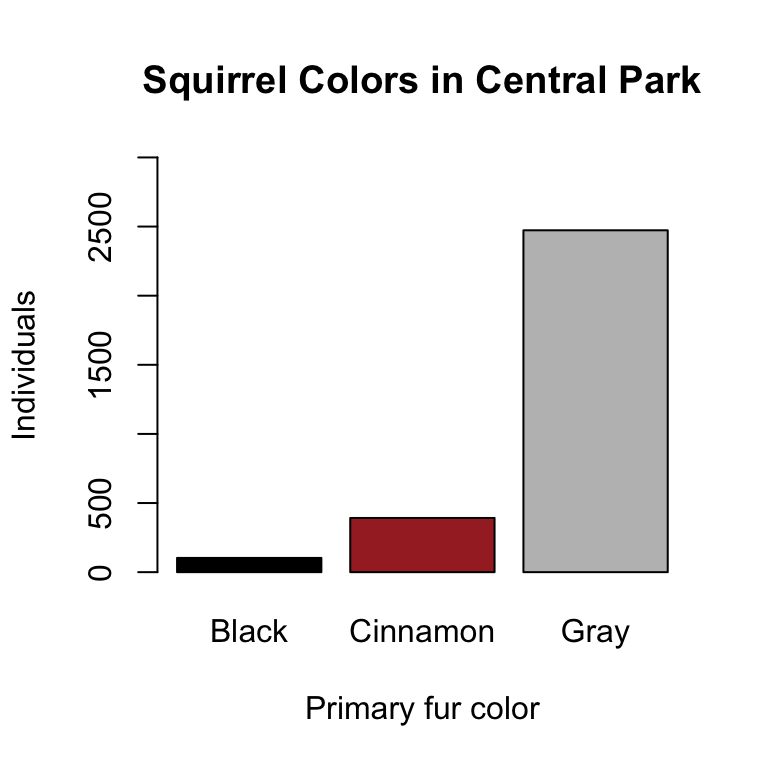
\includegraphics{Research-Design---Statistics_files/figure-latex/c3c66-1} \end{center}

This graph has two axes, the horizontal x-axis and the vertical y-axis. We see the categories of primary fur color on the x-axis and the frequencies of each category on the y-axis. Graphical functions in R aren't all that complex, but the often have a lot of arguments providing the user with options to customize different aspects of the graph. I've specified several arguments in the function:

\begin{itemize}
\tightlist
\item
  \texttt{ylim:} Controls the scale of the y-axis, which I've specified as 0 for the minimum and 3000 for the maximum.\\
\item
  \texttt{names.arg:}: Allows you to specify names for each category, in the same order as the categories are displayed in the output of the \texttt{table} function.
\item
  \texttt{col:} Specifies the color of each bar. These can be all the same, but in this case, I've specified colors that match the descriptions of the primary fur colors.
\item
  \texttt{xlab:} This controls the text for the x-axis label.
\item
  \texttt{ylab:} Text for the y-axis label. and the remaining arguments are used to add axis and plot titles.
\item
  \texttt{main:} Text for the main title of the graph.
\end{itemize}

There are many more arguments you can use to customize figures in R, and I certainly don't have them all memorized. If you want to adjust something, your best bet is to look at the documentation for the plotting function (?barplot in this case) and search for an argument that allows you to do what you want to do!

Note that the bar graph above shows the frequencies of each category of primary fur color, but before I made the point that raw frequences aren't that informative on their own, and that we should generally quantify proportions to characterize the distribution of categorical data. We can easy display the proportions instead of the frequencies, again by wrapping the \texttt{table} function with the \texttt{prop.table} function:

\begin{Shaded}
\begin{Highlighting}[]
\FunctionTok{barplot}\NormalTok{(}\FunctionTok{prop.table}\NormalTok{(}\FunctionTok{table}\NormalTok{(sq}\SpecialCharTok{$}\NormalTok{primary.fur.color)), }
        \AttributeTok{ylim=}\FunctionTok{c}\NormalTok{(}\DecValTok{0}\NormalTok{, }\DecValTok{1}\NormalTok{),}
        \AttributeTok{names.arg =} \FunctionTok{c}\NormalTok{(}\StringTok{"Black"}\NormalTok{, }\StringTok{"Cinnamon"}\NormalTok{, }\StringTok{"Gray"}\NormalTok{),}
        \AttributeTok{col=}\FunctionTok{c}\NormalTok{(}\StringTok{"black"}\NormalTok{, }\StringTok{"brown"}\NormalTok{, }\StringTok{"gray"}\NormalTok{),}
        \AttributeTok{xlab=}\StringTok{"Primary fur color"}\NormalTok{, }\AttributeTok{ylab=}\StringTok{"Proportion"}\NormalTok{, }
        \AttributeTok{main=}\StringTok{"Squirrel Colors in Central Park"}\NormalTok{)}
\end{Highlighting}
\end{Shaded}

\begin{center}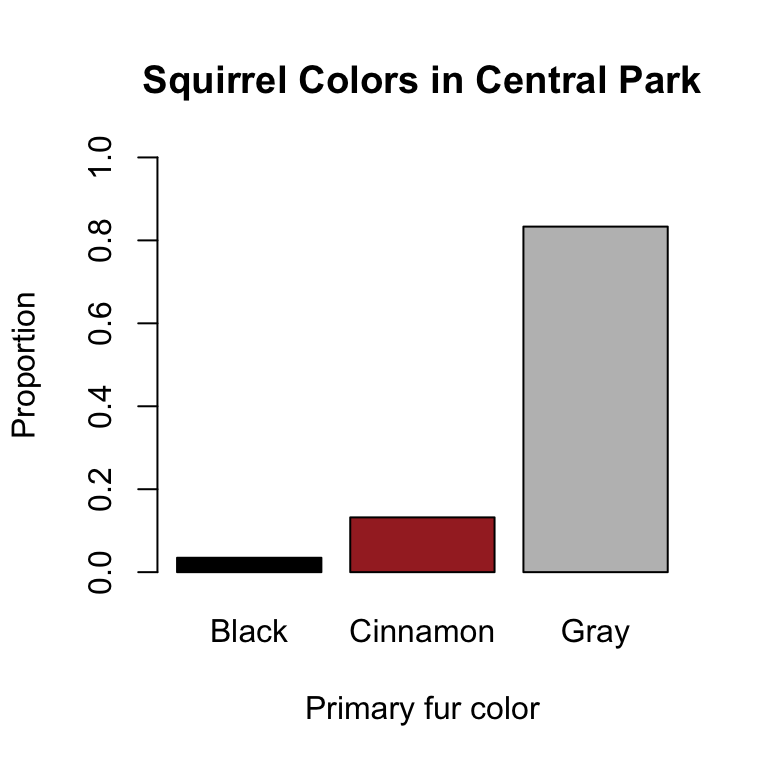
\includegraphics{Research-Design---Statistics_files/figure-latex/c3c67-1} \end{center}

And that's basically it for a basic description of the observed distribution for a categorical variable!

\subsection{Describing distributions of quantitative variables}\label{describing-distributions-of-quantitative-variables}

Let's turn our attention to describing quantitative variables. For this example we'll go back to our dataset on tail autotomy. We start by loading the data and naming the dataframe \texttt{tail} and looking at the structure of the dataframe::

\begin{Shaded}
\begin{Highlighting}[]
\SpecialCharTok{\textgreater{}} 
\ErrorTok{\textgreater{}}\NormalTok{ tail }\OtherTok{\textless{}{-}} \FunctionTok{read.csv}\NormalTok{(}\StringTok{"data/plci\_tails.csv"}\NormalTok{)}
\SpecialCharTok{\textgreater{}} 
\ErrorTok{\textgreater{}} \FunctionTok{str}\NormalTok{(tail)}
\StringTok{\textquotesingle{}data.frame\textquotesingle{}}\SpecialCharTok{:}   \DecValTok{40}\NormalTok{ obs. of  }\DecValTok{8}\NormalTok{ variables}\SpecialCharTok{:}
 \ErrorTok{$}\NormalTok{ individual}\SpecialCharTok{:}\NormalTok{ chr  }\StringTok{"16O300"} \StringTok{"16O301"} \StringTok{"16O302"} \StringTok{"16O303"}\NormalTok{ ...}
 \SpecialCharTok{$}\NormalTok{ morph     }\SpecialCharTok{:}\NormalTok{ chr  }\StringTok{"striped"} \StringTok{"striped"} \StringTok{"striped"} \StringTok{"striped"}\NormalTok{ ...}
 \SpecialCharTok{$}\NormalTok{ tail.sec  }\SpecialCharTok{:}\NormalTok{ int  }\DecValTok{110} \DecValTok{160} \DecValTok{250} \DecValTok{360} \DecValTok{220} \DecValTok{120} \DecValTok{310} \DecValTok{220} \DecValTok{360} \DecValTok{410}\NormalTok{ ...}
 \SpecialCharTok{$}\NormalTok{ tail.vel  }\SpecialCharTok{:}\NormalTok{ num  }\DecValTok{3} \FloatTok{2.3} \FloatTok{2.8} \FloatTok{3.3} \FloatTok{4.6} \DecValTok{3} \FloatTok{3.5} \FloatTok{2.6} \FloatTok{2.4} \FloatTok{2.6}\NormalTok{ ...}
 \SpecialCharTok{$}\NormalTok{ mass.g    }\SpecialCharTok{:}\NormalTok{ num  }\FloatTok{0.8} \FloatTok{0.7} \FloatTok{0.9} \DecValTok{1} \FloatTok{0.6} \FloatTok{0.6} \FloatTok{1.2} \FloatTok{0.8} \FloatTok{0.7} \FloatTok{0.9}\NormalTok{ ...}
 \SpecialCharTok{$}\NormalTok{ length.cm }\SpecialCharTok{:}\NormalTok{ num  }\FloatTok{3.9} \DecValTok{4} \FloatTok{3.9} \DecValTok{4} \FloatTok{3.4} \FloatTok{3.3} \FloatTok{4.2} \FloatTok{3.7} \FloatTok{3.6} \FloatTok{3.8}\NormalTok{ ...}
 \SpecialCharTok{$}\NormalTok{ easting   }\SpecialCharTok{:}\NormalTok{ int  }\DecValTok{350827} \DecValTok{350827} \DecValTok{350831} \DecValTok{350831} \DecValTok{350831} \DecValTok{352128} \DecValTok{352121} \DecValTok{352122} \DecValTok{352116} \DecValTok{352119}\NormalTok{ ...}
 \SpecialCharTok{$}\NormalTok{ northing  }\SpecialCharTok{:}\NormalTok{ int  }\DecValTok{4699989} \DecValTok{4699989} \DecValTok{4699988} \DecValTok{4699988} \DecValTok{4699988} \DecValTok{4702166} \DecValTok{4702172} \DecValTok{4702174} \DecValTok{4702169} \DecValTok{4702170}\NormalTok{ ...}
\end{Highlighting}
\end{Shaded}

Here we see 40 observations of eight variables, as expected. Let's start by examining the distribution of initial tail velocity, which is the number of oscillations of the tail per second after being severed. Characterizing the distribution of a quantitative varible is more involved than for a qualitative variable. When we were describing the primary fur color of squirrels, we could easily compute the proportion of each fur color in the dataset, creating a probability distribution. That was an easy task because categories are discrete units. Quantitative variables, on the other hand, are more tricky because often the data are not discrete. How many salamanders will have an initial velocity of 2.3 oscillations per second? Probably not many! Even if the quantitative variable is discrete (integers), such as tail movement time measured in seconds, there are often very few observations of each particular value.

Let's look at some graphs to show you waht I mean. The distribution of a single quantitative variabe is often displayed as a histogram. Here's an example for the initial tail velocity:

\begin{Shaded}
\begin{Highlighting}[]
\FunctionTok{hist}\NormalTok{(tail}\SpecialCharTok{$}\NormalTok{tail.vel, }
     \AttributeTok{col =} \StringTok{"skyblue"}\NormalTok{,}
     \AttributeTok{main=}\StringTok{""}\NormalTok{,}
     \AttributeTok{xlab=}\StringTok{"Initial velocity (oscillations/sec)"}\NormalTok{, }\AttributeTok{ylab=}\StringTok{"Number of individuals"}\NormalTok{)}
\end{Highlighting}
\end{Shaded}

\begin{center}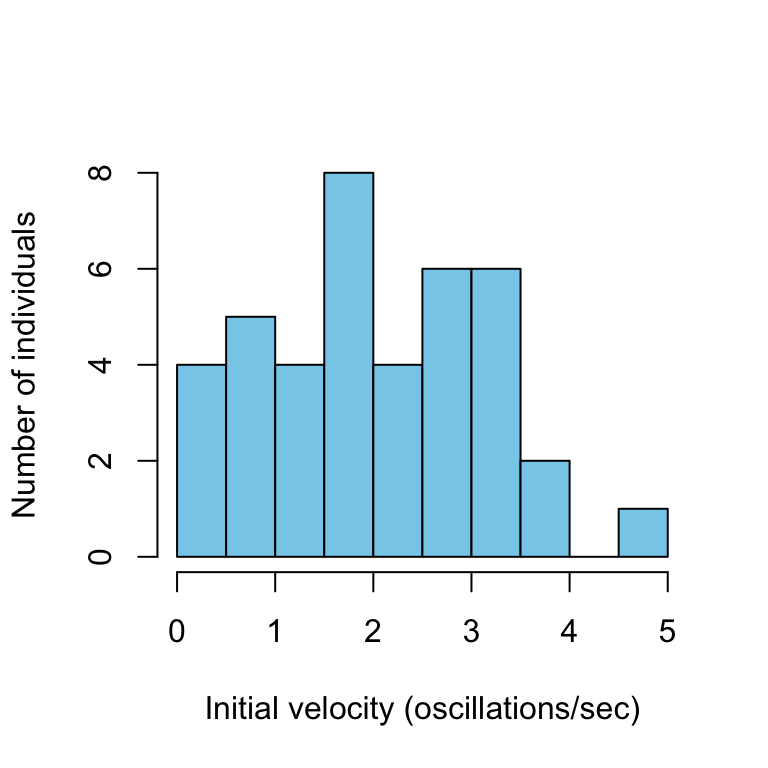
\includegraphics{Research-Design---Statistics_files/figure-latex/c3c69-1} \end{center}

A histogram combines multiple observations that have similar values (x-axis) and shows the frequency of those values (y-axis). The size of the bins in the histogram above are 0.5 oscillations/sec.~For example, we can see there were 4 salamanders with 0-0.5 oscillations/sec, 5 with 0.5-1 oscillations/sec, and so on. The size of the bins is automatically computed with an algorithm, but you could specify the size with the \texttt{breaks} argument. I find the easiest way to specify the breaks is by writing a vector of exactly where I want to breaks. For example, suppose I want breaks every 0.25 units. I can see based on the histogram above that the observations are between 0 and 5, so I want to create breaks every 0.25 units between 0 and 5. I can do this with the \texttt{seq} function. Below are two alternative version of histograms of the same dataset but with bins that are either 0.25 units wide or 0.1 units wide:

\begin{Shaded}
\begin{Highlighting}[]
\FunctionTok{par}\NormalTok{(}\AttributeTok{mfrow=}\FunctionTok{c}\NormalTok{(}\DecValTok{1}\NormalTok{,}\DecValTok{2}\NormalTok{))}
\FunctionTok{hist}\NormalTok{(tail}\SpecialCharTok{$}\NormalTok{tail.vel, }
     \AttributeTok{col =} \StringTok{"skyblue"}\NormalTok{, }\AttributeTok{breaks =} \FunctionTok{seq}\NormalTok{(}\DecValTok{0}\NormalTok{, }\DecValTok{5}\NormalTok{, }\AttributeTok{by =} \FloatTok{0.25}\NormalTok{),}
     \AttributeTok{main =} \StringTok{"Bin size: 0.25 oscillations/sec"}\NormalTok{,}
     \AttributeTok{xlab=}\StringTok{"Initial velocity (oscillations/sec)"}\NormalTok{, }\AttributeTok{ylab=}\StringTok{"Number of individuals"}\NormalTok{)}

\FunctionTok{hist}\NormalTok{(tail}\SpecialCharTok{$}\NormalTok{tail.vel, }
     \AttributeTok{col =} \StringTok{"skyblue"}\NormalTok{, }\AttributeTok{breaks =} \FunctionTok{seq}\NormalTok{(}\DecValTok{0}\NormalTok{, }\DecValTok{5}\NormalTok{, }\AttributeTok{by =} \FloatTok{0.1}\NormalTok{),}
     \AttributeTok{main =} \StringTok{"Bin size: 0.1 oscillations/sec"}\NormalTok{,}
     \AttributeTok{xlab=}\StringTok{"Initial velocity (oscillations/sec)"}\NormalTok{, }\AttributeTok{ylab=}\StringTok{"Number of individuals"}\NormalTok{)}
\end{Highlighting}
\end{Shaded}

\begin{center}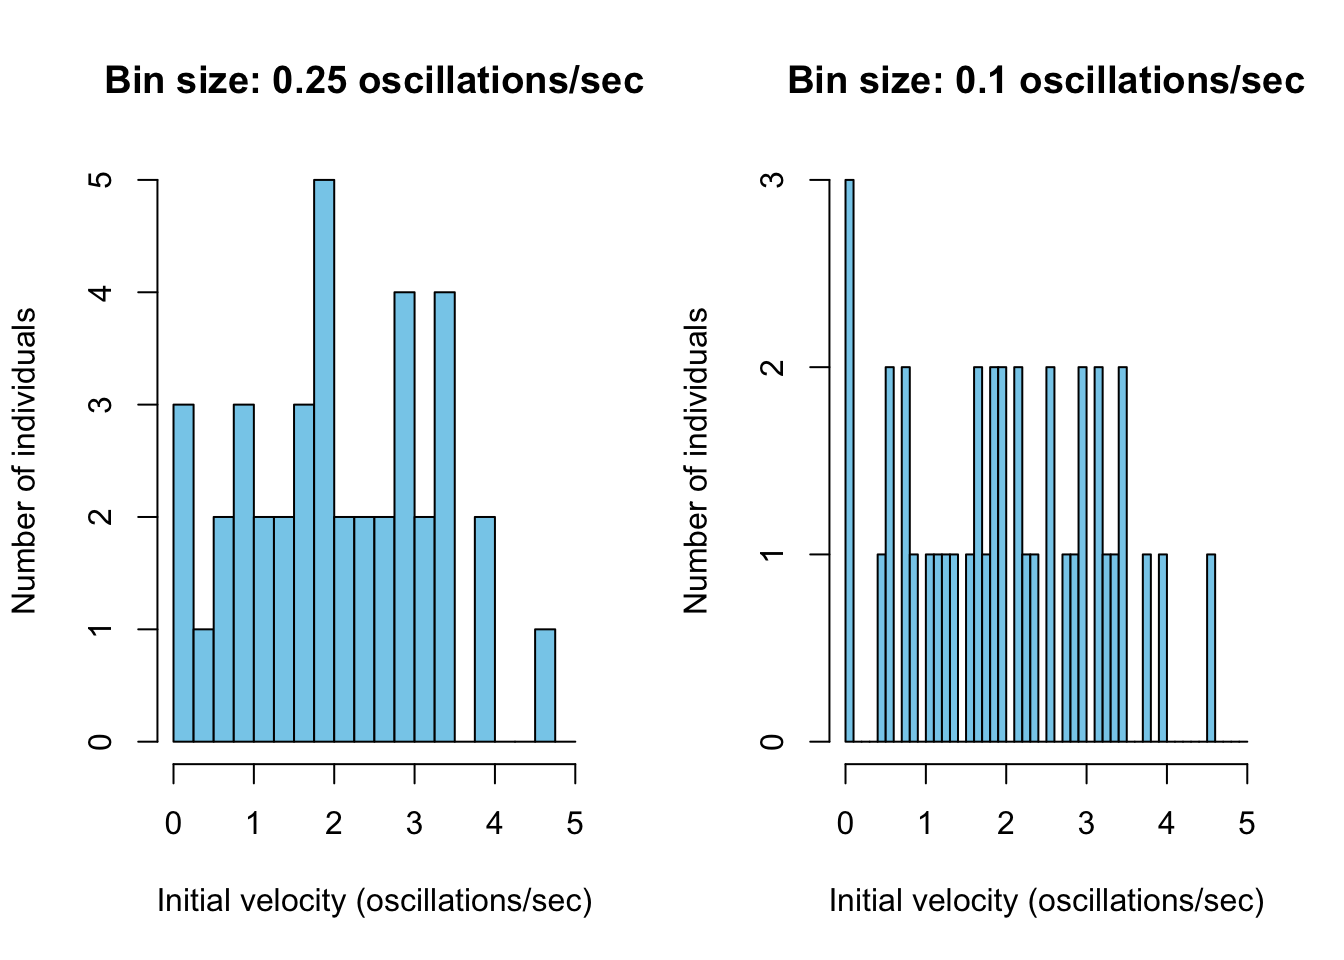
\includegraphics[width=0.85\linewidth]{Research-Design---Statistics_files/figure-latex/c3c70-1} \end{center}

You can see that histograms become less effective for displaying the variation in the data when the bin size gets smaller and smaller, with more observations of 0 salamanders in particular bins. That's a feature of quantitative data. Because numeric variables can be measured to decimal points, there are few observations of any particular value. If the data are measured very precisely and the bin size is smaller than the precision of the data, you'll end up with a histogram showing separate bars for each observation, each with a frequency of a one. That's not helpful. A good rule of thumb is to keep the bin size large enough such that there are few gaps (frequencies of zero) within the range of the observations.

Like qualitative data, it is helpful to characterize the probability distribution of the observations, but again that is made challenging by the fine scale of the observations. What is the probability of initial velocity being 3.213512343243 oscillations/sec? Infinitely small! To resolve this issue, we quantify the \textbf{probability density}, which is the probability that an observation falls within a range of values. Here's the same histogram as our initial histogram, but instead of the y-axis showing frequencies, it now shows probability densities by specifying the \texttt{freq} argument to FALSE:

\begin{Shaded}
\begin{Highlighting}[]
\FunctionTok{hist}\NormalTok{(tail}\SpecialCharTok{$}\NormalTok{tail.vel, }\AttributeTok{freq =} \ConstantTok{FALSE}\NormalTok{,}
     \AttributeTok{col =} \StringTok{"skyblue"}\NormalTok{,}
     \AttributeTok{main=}\StringTok{""}\NormalTok{,}
     \AttributeTok{xlab=}\StringTok{"Initial velocity (oscillations/sec)"}\NormalTok{, }\AttributeTok{ylab=}\StringTok{"Probability density"}\NormalTok{)}
\end{Highlighting}
\end{Shaded}

\begin{center}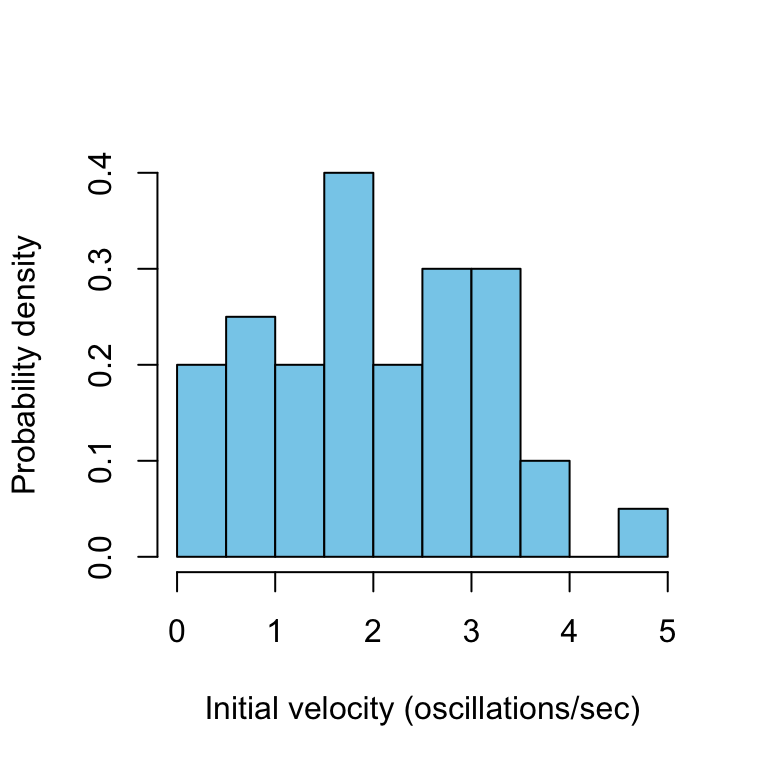
\includegraphics{Research-Design---Statistics_files/figure-latex/c3c71-1} \end{center}

Note that probability \textbf{density} is not the same as a probability. For example, the probability density of initial velocity observations between 1.5 and 2.0 is 0.4. The probability of observations within a particular range, like 1.5 to 2.0 is the area under the probability density curve, in this case \(0.4*0.5 = 0.2\). Indeed 8 out of 40 individuals had an observation between 1.5 and 2, which is 20\%.

Let's crawl out of the weeds a bit. At this point, you basically need to know that characterizing the distribution of a variable requires quantifying the relative probability of different observations, and the way we do that differs between quantitative and qualitative variables.

\subsection{Metrics of central tendency}\label{metrics-of-central-tendency}

Distributions of quantitative variables contain a lot of information, and so it can be helpful to summarize the distributions numerically. One aspect of a distribution is its \textbf{central tendency}. In other words, what are the typical values of a variable? One numeric summary of central tendency is the \textbf{mean}:

\[
\hat{\mu} = \frac{\sum_{i=1}^n x_i}{n},
\]
where \(\hat{\mu}\) is the estimated mean of the variable, \(x_i\) is each observed value of the variable, and \(n\) is the total number of observations. The Greek letter sigma is mathematical notation for summation. The formula basically says to quantify the mean, you need to sum the value of each observation \emph{i} in the dataset, then divide by the total number of observations. The \emph{i} is simply a subscript reprensenting each observation of the variable, from the first (\(i = 1\)) to the last (\(i = n\)). For example, if we have a dataset of \{3, 5, 7, 9, 10\}, the mean is quantified as

\[
\hat{\mu} = \frac{3+5+7+9+10}{5}=6.8
\]

In R, the mean can be quantified with the \texttt{mean} function:

\begin{Shaded}
\begin{Highlighting}[]
\NormalTok{(}\DecValTok{3}\SpecialCharTok{+}\DecValTok{5}\SpecialCharTok{+}\DecValTok{7}\SpecialCharTok{+}\DecValTok{9}\SpecialCharTok{+}\DecValTok{10}\NormalTok{)}\SpecialCharTok{/}\DecValTok{5}
\end{Highlighting}
\end{Shaded}

\begin{verbatim}
## [1] 6.8
\end{verbatim}

\begin{Shaded}
\begin{Highlighting}[]
\FunctionTok{mean}\NormalTok{(}\FunctionTok{c}\NormalTok{(}\DecValTok{3}\NormalTok{,}\DecValTok{5}\NormalTok{,}\DecValTok{7}\NormalTok{,}\DecValTok{9}\NormalTok{,}\DecValTok{10}\NormalTok{))}
\end{Highlighting}
\end{Shaded}

\begin{verbatim}
## [1] 6.8
\end{verbatim}

Let's now go ahead and quantify the mean initial velocity for salamander tails. We can do this by applying the mean function to the variable \texttt{tail.vel} in the tails data frame:

\begin{Shaded}
\begin{Highlighting}[]
\FunctionTok{mean}\NormalTok{(tail}\SpecialCharTok{$}\NormalTok{tail.vel)}
\end{Highlighting}
\end{Shaded}

\begin{verbatim}
## [1] 2.0575
\end{verbatim}

Another common metric of central tendency is the \textbf{median}, which is the middle value of a distribution. Consider again the made-up dataset of \{3, 5, 7, 9, 10\}. The value in the middle is 7, so that's the median. If there's an even number of observations in a dataset, the median can be computed mean of the two middle numbers. For example, if a dataset had observations of \{3, 5, 7, 8, 9, 10\}, the median is the average of 7 and 8: 7.5. The median can be computed with the \texttt{median} function in R. Let's do that for the tail velocity variable:

\begin{Shaded}
\begin{Highlighting}[]
\FunctionTok{median}\NormalTok{(tail}\SpecialCharTok{$}\NormalTok{tail.vel)}
\end{Highlighting}
\end{Shaded}

\begin{verbatim}
## [1] 2
\end{verbatim}

Fascinating. The mean and median tail velocity are very similar, but that's not always the case. Let's quantify the mean and median of the total tail movement time:

\begin{Shaded}
\begin{Highlighting}[]
\FunctionTok{mean}\NormalTok{(tail}\SpecialCharTok{$}\NormalTok{tail.sec)}
\end{Highlighting}
\end{Shaded}

\begin{verbatim}
## [1] 156.25
\end{verbatim}

\begin{Shaded}
\begin{Highlighting}[]
\FunctionTok{median}\NormalTok{(tail}\SpecialCharTok{$}\NormalTok{tail.sec)}
\end{Highlighting}
\end{Shaded}

\begin{verbatim}
## [1] 75
\end{verbatim}

Here we can see the mean of the total tail movement time is 156.25 sec, whereas the median is 75 sec.~That's a huge difference. What gives? It turns out that the similarity of the mean and median depends on the shape of the distribution. Let's compare histograms for tail movement time and tail velocity.

\begin{Shaded}
\begin{Highlighting}[]
\FunctionTok{par}\NormalTok{(}\AttributeTok{mfrow=}\FunctionTok{c}\NormalTok{(}\DecValTok{1}\NormalTok{,}\DecValTok{2}\NormalTok{))}
\FunctionTok{hist}\NormalTok{(tail}\SpecialCharTok{$}\NormalTok{tail.sec,}
     \AttributeTok{col =} \StringTok{"skyblue"}\NormalTok{,}
     \AttributeTok{main=}\StringTok{""}\NormalTok{,}
     \AttributeTok{xlab=}\StringTok{"Total tail movement time (sec)"}\NormalTok{, }\AttributeTok{ylab=}\StringTok{"Individuals"}\NormalTok{)}

\FunctionTok{hist}\NormalTok{(tail}\SpecialCharTok{$}\NormalTok{tail.vel,}
     \AttributeTok{col =} \StringTok{"skyblue"}\NormalTok{,}
     \AttributeTok{main=}\StringTok{""}\NormalTok{,}
     \AttributeTok{xlab=}\StringTok{"Initial velocity (oscillations/sec)"}\NormalTok{, }\AttributeTok{ylab=}\StringTok{"Individuals"}\NormalTok{)}
\end{Highlighting}
\end{Shaded}

\begin{center}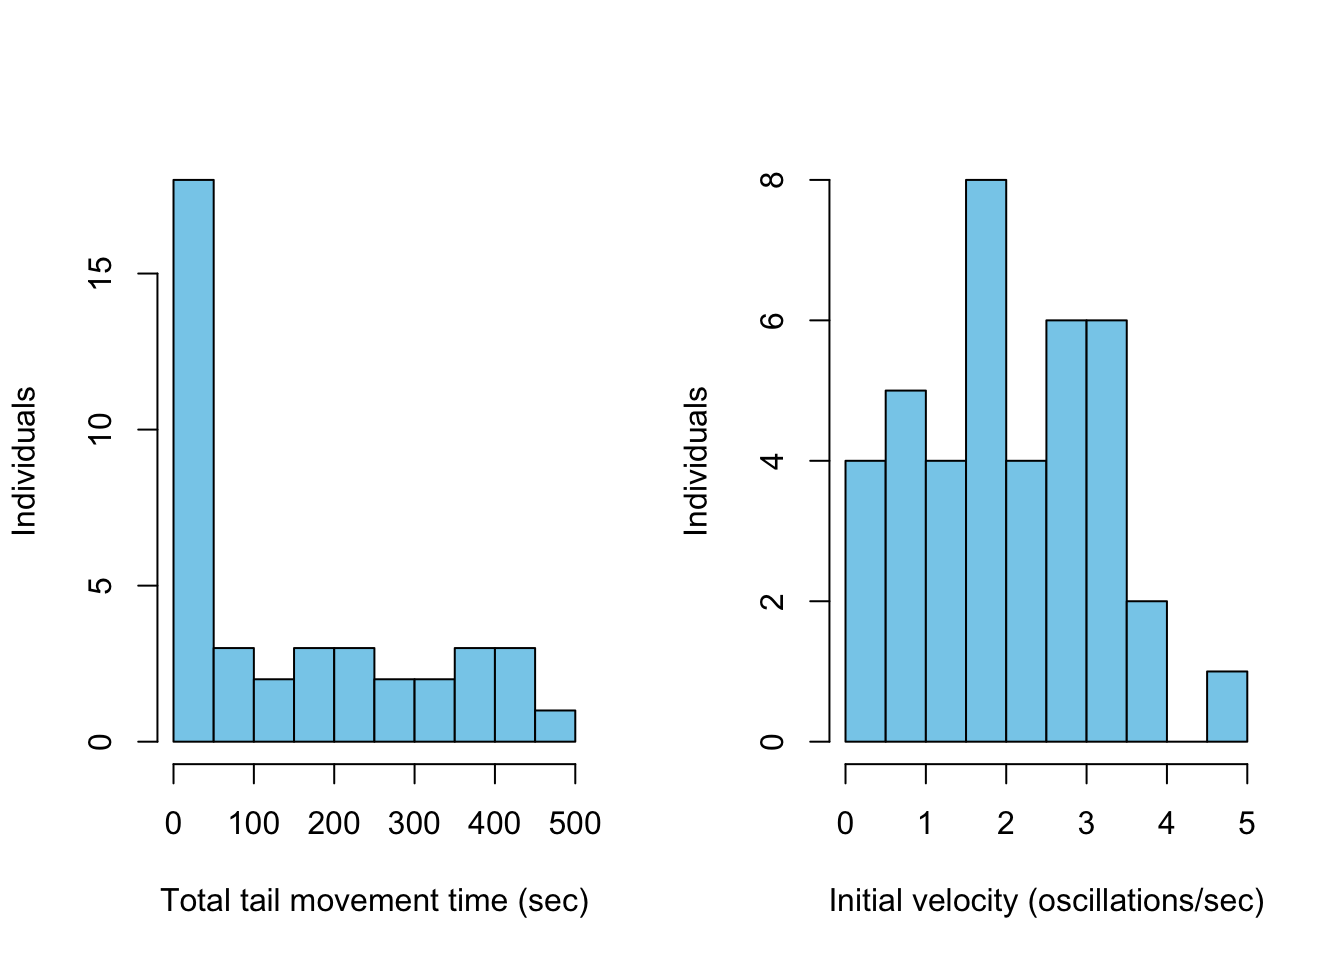
\includegraphics[width=0.85\linewidth]{Research-Design---Statistics_files/figure-latex/c3c76-1} \end{center}

We can see the shape of the two distributions are quite different. The distribution of initial velocity is somewhat bell-shaped, the the majority of observations in the center of the distribution and a minority of observations in both tails of the distribution (i.e., the upper and lower extremes). In contrast, the distribution of total tail movement time is strongly \textbf{skewed}. The most common observations (i.e., the \textbf{mode}) are 0-50 sec, and then there's a long tail of observations to more positive values. There are no observations in the other direction of the mode, which wouldn't make sense because they'd have to be negative. In this case we can describe the distribution as skewed to the riht, or exhibiting positive skew. If the tail extended primarily to more negative values, we can describe the distribution as skewed to the left, or exhibiting negative skew.

\begin{Shaded}
\begin{Highlighting}[]
\FunctionTok{par}\NormalTok{(}\AttributeTok{mfrow=}\FunctionTok{c}\NormalTok{(}\DecValTok{1}\NormalTok{,}\DecValTok{2}\NormalTok{))}
\FunctionTok{hist}\NormalTok{(tail}\SpecialCharTok{$}\NormalTok{tail.vel, }
     \AttributeTok{col =} \StringTok{"skyblue"}\NormalTok{,}
     \AttributeTok{xlab=}\StringTok{"Initial velocity (oscillations/sec)"}\NormalTok{, }\AttributeTok{ylab=}\StringTok{"Number of individuals"}\NormalTok{, }\AttributeTok{main=}\StringTok{""}\NormalTok{)}

\FunctionTok{hist}\NormalTok{(tail}\SpecialCharTok{$}\NormalTok{tail.vel, }\AttributeTok{freq=}\ConstantTok{FALSE}\NormalTok{,}
     \AttributeTok{col =} \StringTok{"skyblue"}\NormalTok{, }
     \AttributeTok{xlab=}\StringTok{"Initial velocity (oscillations/sec)"}\NormalTok{, }\AttributeTok{ylab=}\StringTok{"Probability density"}\NormalTok{, }\AttributeTok{main=}\StringTok{""}\NormalTok{)}
\end{Highlighting}
\end{Shaded}

\begin{center}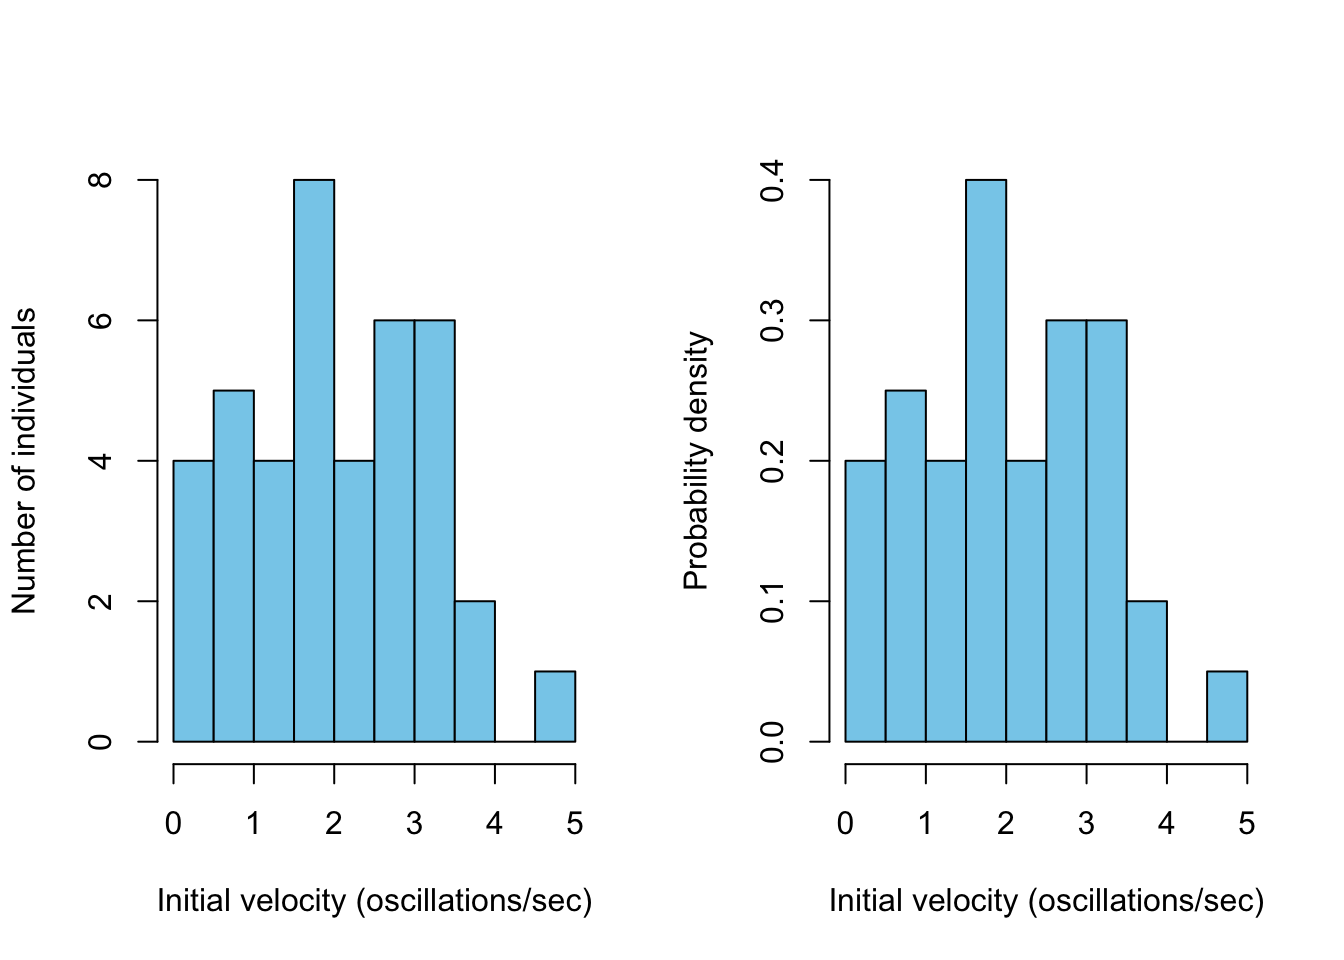
\includegraphics[width=0.85\linewidth]{Research-Design---Statistics_files/figure-latex/c3c77-1} \end{center}

But back to our original point. It turns out the mean and the median are similar to each other for variables with bell-shaped distributions. In fact, if the distribution is perfectly bell-shaped, the mean, median, and mode are all identical. When a variable has a skewed distribution, the mean and median diverge from each other, with the mean being drawn out in the direction of hte skew. The mean is often described as the center of gravity, such that it's sensitive to extreme values. If you change our made-up dataset from \{3, 5, 7, 9, 10\} to \{3, 5, 7, 9, 80\}, the mean changes from 6.8 to 20.8. The median, in contrast, is always the middle observation of the variable. It remains 7 in both datasets.

\subsection{Metrics of variance}\label{metrics-of-variance}

Another way of numerically characterizing a distribution is the variation among observations, which can be quantified with the \textbf{variance}:

\[
\hat{\sigma}^2 = \frac{1}{n-1} \sum_{i=1}^n (x_i - \hat{\mu})^2
\]
Let's take a look at what the variance is doing. We take each observation \(x\), subtract the mean from that value, and then square the term. This value is called a \textbf{squared deviation}, and the variance sums those squared deviations and then divides by the sample size (minus 1). Effectively what's happening here is that the variance is quantifying the mean of the squared deviations from the mean. The more the observations are far away from the mean, the greater the squared deviations, the greater the mean. The variance with our made-up dataset, \{3, 5, 7, 9, 10\}:

\[
\hat{\sigma}^2 = \frac{1}{(5-1)} \left[ (3 - 6.8)^2 + (5 - 6.8)^2 + (7 - 6.8)^2 + (9 - 6.8)^2 + (10 - 6.8)^2 \right] = 8.2
\]
Why is the denominator of the variance \(n-1\) instead of just \(n\)? The quantity \(n-1\) is a bias correction factor when quantifying the variance with a sample of the data. When you only have a subset of observations from the group of interest, the variance tends to be underestimated. More on this in a later chapter when we cover sampling.

In R we can quantify the variance with the \texttt{var} function. Let's apply it to the tail movement and velocity variables:

\begin{Shaded}
\begin{Highlighting}[]
\DocumentationTok{\#\# tail movement time}
\FunctionTok{var}\NormalTok{(tail}\SpecialCharTok{$}\NormalTok{tail.sec)}
\end{Highlighting}
\end{Shaded}

\begin{verbatim}
## [1] 22680.45
\end{verbatim}

\begin{Shaded}
\begin{Highlighting}[]
\DocumentationTok{\#\# initial velocity}
\FunctionTok{var}\NormalTok{(tail}\SpecialCharTok{$}\NormalTok{tail.vel)}
\end{Highlighting}
\end{Shaded}

\begin{verbatim}
## [1] 1.393788
\end{verbatim}

We see the variance in tail movement time is 22680.45 and 1.39 for initial velocity. What are the units? Because we're squaring the deviation of each observation from the mean, the units of variance is the square of the original unit. Thus, the variance of tail movement time is 22680.45 \(sec^2\). Squared units can be difficult to comprehend, but we can put this metric back on the scale of the original units by taking the square root of the variance, which is called the \textbf{standard deviation}:

\[
\hat{\sigma} = \sqrt{\frac{1}{n-1} \sum_{i=1}^n (x_i - \hat{\mu})^2}
\]
The standard deviation can be quantified in R with the \texttt{sd} function:

\begin{Shaded}
\begin{Highlighting}[]
\DocumentationTok{\#\# tail movement time}
\FunctionTok{sd}\NormalTok{(tail}\SpecialCharTok{$}\NormalTok{tail.sec)}
\end{Highlighting}
\end{Shaded}

\begin{verbatim}
## [1] 150.6003
\end{verbatim}

\begin{Shaded}
\begin{Highlighting}[]
\DocumentationTok{\#\# initial velocity}
\FunctionTok{sd}\NormalTok{(tail}\SpecialCharTok{$}\NormalTok{tail.vel)}
\end{Highlighting}
\end{Shaded}

\begin{verbatim}
## [1] 1.180588
\end{verbatim}

We see now that the estimated standard deviation is 150.6 sec for tail movement time and 1.18 oscillations/sec for initial velocity.

\subsection{Percentiles}\label{percentiles}

One last numerical summary of distributions you should be aware of is the \textbf{percentile}, which is defined as the observation in the dataset for which a specified percentage of the data falls below that value. We've actually already seen a percentile. The median is the 50th percentile because 50\% of the observations fall below that value. But you can quantify a percentile for any level of percentage. In R, percentiles are quantified with the \texttt{quantile} function (quantile is a synonymous term for percentile). Here are some percentiles for the tail velocity data:

\begin{Shaded}
\begin{Highlighting}[]
\DocumentationTok{\#\# Report just the 50th percentile (i.e., the median)}
\FunctionTok{quantile}\NormalTok{(tail}\SpecialCharTok{$}\NormalTok{tail.vel, }\AttributeTok{probs =} \FloatTok{0.5}\NormalTok{)}
\end{Highlighting}
\end{Shaded}

\begin{verbatim}
## 50% 
##   2
\end{verbatim}

\begin{Shaded}
\begin{Highlighting}[]
\DocumentationTok{\#\# Report the 0th, 25th, 50th, 75th, and 100th percentiles:}
\FunctionTok{quantile}\NormalTok{(tail}\SpecialCharTok{$}\NormalTok{tail.vel, }\AttributeTok{probs=}\FunctionTok{c}\NormalTok{(}\DecValTok{0}\NormalTok{, }\FloatTok{0.25}\NormalTok{, }\FloatTok{0.5}\NormalTok{, }\FloatTok{0.75}\NormalTok{, }\DecValTok{1}\NormalTok{))}
\end{Highlighting}
\end{Shaded}

\begin{verbatim}
##    0%   25%   50%   75%  100% 
## 0.000 1.175 2.000 3.000 4.600
\end{verbatim}

So we can see that there are no observations below 0, 25\% of the observations are below 1.175, 50\% of the observations are below 2, etc. Note that the 0th and 100th percentiles are the \textbf{minimum} and \textbf{maximum} observations in the data, respectively.

The quantiles are sometimes used to describe variation in the data. Two common metrics are the \textbf{range} and the \textbf{interquartile range (IQR)}. The range is simply the difference between the maximum and minimum observation, whereas the IQR is the difference between the 75th and 25th percentiles. Here are some relevant R functions that you'll find of use:

\begin{Shaded}
\begin{Highlighting}[]
\DocumentationTok{\#\# report the minimum and maximum}
\FunctionTok{range}\NormalTok{(tail}\SpecialCharTok{$}\NormalTok{tail.vel)}
\end{Highlighting}
\end{Shaded}

\begin{verbatim}
## [1] 0.0 4.6
\end{verbatim}

\begin{Shaded}
\begin{Highlighting}[]
\DocumentationTok{\#\# report the range as max {-} min}
\FunctionTok{max}\NormalTok{(tail}\SpecialCharTok{$}\NormalTok{tail.vel) }\SpecialCharTok{{-}} \FunctionTok{min}\NormalTok{(tail}\SpecialCharTok{$}\NormalTok{tail.vel)}
\end{Highlighting}
\end{Shaded}

\begin{verbatim}
## [1] 4.6
\end{verbatim}

\begin{Shaded}
\begin{Highlighting}[]
\DocumentationTok{\#\# IQR}
\FunctionTok{IQR}\NormalTok{(tail}\SpecialCharTok{$}\NormalTok{tail.vel)}
\end{Highlighting}
\end{Shaded}

\begin{verbatim}
## [1] 1.825
\end{verbatim}

\begin{Shaded}
\begin{Highlighting}[]
\DocumentationTok{\#\# IQR calculated with the quantile function}
\FunctionTok{quantile}\NormalTok{(tail}\SpecialCharTok{$}\NormalTok{tail.vel, }\AttributeTok{probs =} \FloatTok{0.75}\NormalTok{) }\SpecialCharTok{{-}} \FunctionTok{quantile}\NormalTok{(tail}\SpecialCharTok{$}\NormalTok{tail.vel, }\AttributeTok{probs =} \FloatTok{0.25}\NormalTok{) }
\end{Highlighting}
\end{Shaded}

\begin{verbatim}
##   75% 
## 1.825
\end{verbatim}

The range is commonly reported for variables to define the bounds of the observed data, but note that the range will be strongly sensitive to extreme observations. For distributions with extreme observations or strong skew, the IQR can be a useful summary statistic to describe variation. Both the range and the IQR have the same units as the original variable.

\subsection{Summary function}\label{summary-function}

The \texttt{summary} function is handy for quickly evaluating the quantiles and mean of a numeric variable. You can apply it to a single vector, or to an entire data frame to summarize all the objects in the data frame at once. If there are characters in the data frame, the \texttt{summary} function will simply indicate that the object is a character of a specific length.

\begin{Shaded}
\begin{Highlighting}[]
\DocumentationTok{\#\# Summary for a single variable}
\FunctionTok{summary}\NormalTok{(tail}\SpecialCharTok{$}\NormalTok{tail.vel)}
\end{Highlighting}
\end{Shaded}

\begin{verbatim}
##    Min. 1st Qu.  Median    Mean 3rd Qu.    Max. 
##   0.000   1.175   2.000   2.058   3.000   4.600
\end{verbatim}

\begin{Shaded}
\begin{Highlighting}[]
\DocumentationTok{\#\# Summary for the entire data frame}
\FunctionTok{summary}\NormalTok{(tail)}
\end{Highlighting}
\end{Shaded}

\begin{verbatim}
##   individual           morph              tail.sec        tail.vel         mass.g         length.cm        easting          northing      
##  Length:40          Length:40          Min.   :  0.0   Min.   :0.000   Min.   :0.3000   Min.   :2.800   Min.   :350789   Min.   :4699969  
##  Class :character   Class :character   1st Qu.: 37.5   1st Qu.:1.175   1st Qu.:0.5000   1st Qu.:3.300   1st Qu.:350836   1st Qu.:4700003  
##  Mode  :character   Mode  :character   Median : 75.0   Median :2.000   Median :0.6500   Median :3.600   Median :350952   Median :4700080  
##                                        Mean   :156.2   Mean   :2.058   Mean   :0.6975   Mean   :3.607   Mean   :351311   Mean   :4700773  
##                                        3rd Qu.:277.5   3rd Qu.:3.000   3rd Qu.:0.8250   3rd Qu.:3.925   3rd Qu.:352089   3rd Qu.:4702130  
##                                        Max.   :460.0   Max.   :4.600   Max.   :1.2000   Max.   :4.400   Max.   :352130   Max.   :4702177
\end{verbatim}

\section{Describing relationships between variables}\label{describing-relationships-between-variables}

Whether your goal is causal explanation or prediction, much of science involves examining relationships between variables. So far we have looked at different ways of describing a single variable. But perhaps the distribution of a variable depends on the value of another variable. We need some basic approaches to describe associations between variables

\subsection{Associations between quantitative variables}\label{associations-between-quantitative-variables}

Does learning something about the length of salamanders tell us anything about their mass? Both length and mass are quantitative variables. The first step to examine the association between two quantitative variables is to create a \textbf{scatterplot}, where each point in the graph displays the values of the two varialbes for each individual in the dataset.

You can create a scatterplot with the \texttt{plot} command in R. The first argument of the plot command asks for the variables. You can either enter the variables separated by a comma (x, y), or you can use a tilde to relate the y to the x variable (y \textasciitilde{} x). Either is fine, but I generally tend to use the tilde format. Note again there are additional arguments to enter x and y axis labels (\texttt{xlab}, \texttt{ylab}), the type of the points (\texttt{pch}), etc. All of the arguments can be viewed with ?plot. Here's the relationship between mass and length:

\begin{Shaded}
\begin{Highlighting}[]
\FunctionTok{plot}\NormalTok{(tail}\SpecialCharTok{$}\NormalTok{mass.g }\SpecialCharTok{\textasciitilde{}}\NormalTok{ tail}\SpecialCharTok{$}\NormalTok{length.cm, }\AttributeTok{asp=}\DecValTok{1}\NormalTok{,}
     \AttributeTok{xlab=}\StringTok{"Snout{-}vent length (cm)"}\NormalTok{, }\AttributeTok{ylab=}\StringTok{"Mass (g)"}\NormalTok{, }\AttributeTok{main=}\StringTok{""}\NormalTok{,}
     \AttributeTok{pch =} \DecValTok{19}\NormalTok{) }\CommentTok{\#pch changes the type of plotting character}
\end{Highlighting}
\end{Shaded}

\begin{center}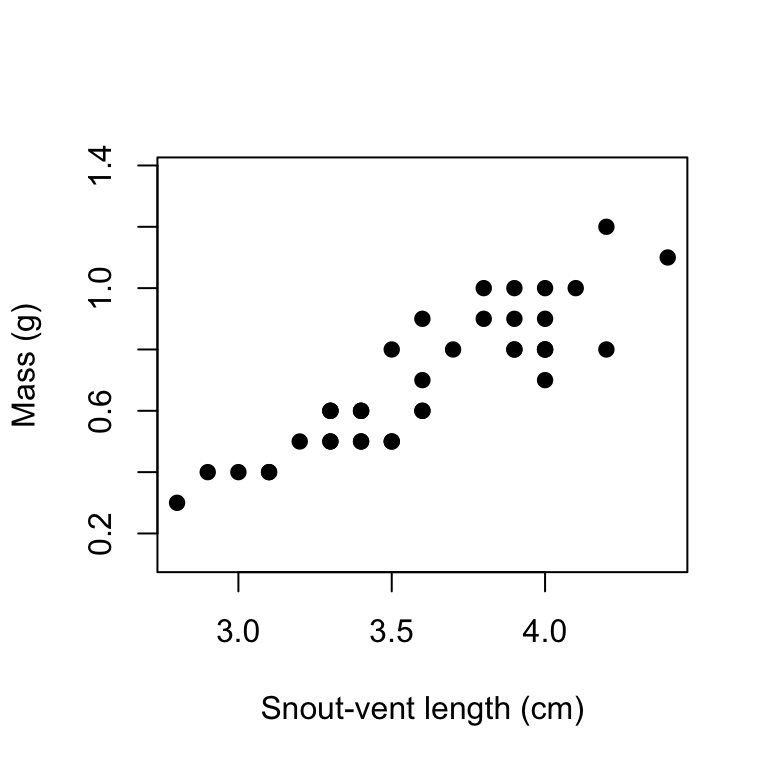
\includegraphics{Research-Design---Statistics_files/figure-latex/c3c83-1} \end{center}

The scatterplot shows a clear pattern. When an individuals length is low, their mass tends to be low as well. When an individual's length is high, their mass tends to be high as well. In other words, there appears to be a positive relationship between mass and length. Scatterplots can also reveal a negative relationships, where the value of one variable tends to decrease as the value of the other variable increases.

The figure below shows a range of possible patterns that one might encounter in scatterplots. Note that in addition to describing the nature of the relationship between variables, we can also describe the magnitude of the relationship. For example, the graph shows two positive relationships in the top row, but the pattern looks much stronger in the scatterplot on the left than the scatterplot on the right.

\begin{center}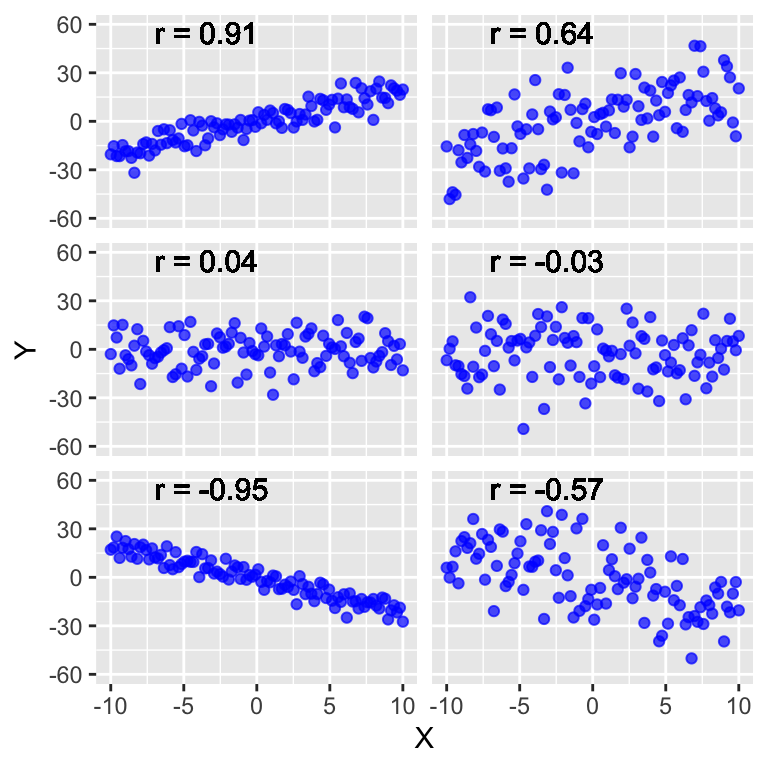
\includegraphics{Research-Design---Statistics_files/figure-latex/c3c84-1} \end{center}

The \textbf{correlation coefficient (r)} is a numerical metric used to describe both the direction and strength of an association. It has a bit of a messy formula:

\[
r = \frac{\frac{1}{n-1} \sum_{i=1}^n (x_i - \hat{\mu}_x)(y_i - \hat{\mu}_y)}{\hat{\sigma}_x \hat{\sigma}_y}
\]
I don't want to get into the mathemeatical details here, but at a very basic level, the correlation coefficient is based on the \textbf{covariance}, which is the numerator in the formula for the correlation coefficient. The covariance is a cross product of the deviation between each value of variables \(x\) and \(y\) from their mean. When \(x\) and \(y\) values have a common relationship to their mean, the covariance is positive. This would reflect a positive association, where high values of \(x\) correspond to high values of \(y\), and vice versa. When \(x\) and \(y\) values have opposite relationship to their mean, the covariance is negative. This would reflect a negative association, where high values of \(x\) correspond to low values of \(y\), and vice versa. When there's no association between \(x\) and \(y\), the covariance is 0. Covariance has awkward units. The correlation coefficint divides the covariance by the standard deviations of each variable, which standardizes the association to be between -1 and 1. Negative values reflect negative associations, positive values reflect positive associations, and \(r=0\) reflects no association. The strength of the association is reflected by how close the value of \(r\) is to 1 or -1. Stronger associations have values of \(r\) close to 1 or -1. You can see this in the example scatterplots, where stronger associations reflect less scatter among the points. When \(r\) is exactly 1 or -1, the points all fall on a perfect line.

Does it matter which variable we place on each axis when examining the association between two quantitative variables? It can. If your goal is causal explanation, you should generally place the explanatory variable on the x-axis and the repsonse variable on the y-axis. The length of an animal is almost certainly one cause of its mass, so it makes sense that we placed length on the x-axis. But don't assume that an association between two variables is causal! When we describe associations between variables, all we are doing is describing patterns. We'll need additional tools to say whether or not the patterns we find in the data reflect some kind of causal process. More on that in later chapters.

\subsection{Associations between quantitative and qualitative variables}\label{associations-between-quantitative-and-qualitative-variables}

For now I'll show you two ways of graphically comparing quantitative data between categories of a qualitative variable. The idea here is to visually inspect how the distribution of the quantitative variable differs between categories of the qualitative variable. For example, let's compare initial velocity of tail movement between the color morphs. One approach is to generate a \textbf{box plot} to simply compare the distributions of velocity between morphs:

\begin{Shaded}
\begin{Highlighting}[]
\FunctionTok{boxplot}\NormalTok{(tail}\SpecialCharTok{$}\NormalTok{tail.vel }\SpecialCharTok{\textasciitilde{}}\NormalTok{ tail}\SpecialCharTok{$}\NormalTok{morph, }\AttributeTok{col=}\FunctionTok{c}\NormalTok{(}\StringTok{"firebrick"}\NormalTok{, }\StringTok{"gray"}\NormalTok{),}
        \AttributeTok{xlab=}\StringTok{"Color morph"}\NormalTok{, }\AttributeTok{ylab=}\StringTok{"Oscillations/sec"}\NormalTok{)}
\end{Highlighting}
\end{Shaded}

\begin{center}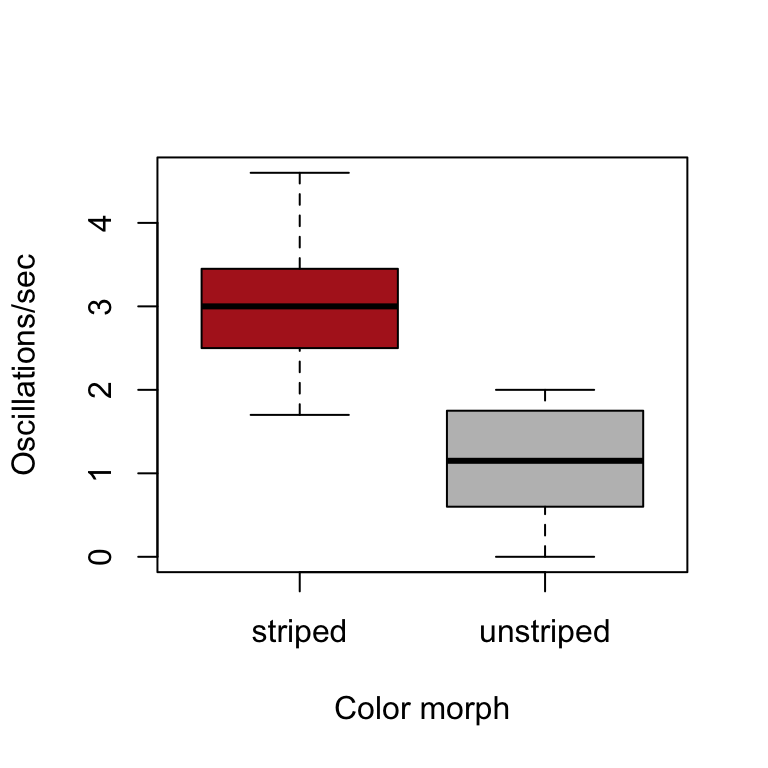
\includegraphics{Research-Design---Statistics_files/figure-latex/c3c85-1} \end{center}

Boxplots provide an alternative visual representation of the distribution of a quantitative varaible by displaying particular numerical summaries:

\begin{itemize}
\item
  Median: represented by the thick horizontal line as a metric of central tendency.
\item
  IQR: represented by the edges of the box, where the lower edge is the 25th percentile and the upper edge is the 75th percentile. The box displays the bounds of the middle 50\% of the data, giving you a sense for variation.
\item
  Variation in the tails: Values in the tails of the distribution are displayed by the whiskers, which extend up to 1.5 times the IQR from the box. Any values outside the whiskers are defined as \textbf{outliers} and are displayed by points.
\end{itemize}

The shape of a distribution can be inferred from a box plot based on the symmetry of the box and whiskers. If the box and whiskers are largely symmetrical, then the distribution has a bell shape. If the box and whisker extends far from the median to one end of the distribution, then the distribution is skewed.

So what does all this mean for comparing initial velocity between color morphs? We can see that the shape of the initial velocity distribution is similar between color morphs, being bell-shaped for both morphs. The variation among individuals also appears largely consistent between morphs. Clearly, however, the distribution of initial velocity differ dramatically in central tendency. The distribution of initial velocity is shifted to greater values for the striped morph than the unstriped morph.

One of the downsides of boxplots is that you don't see the individual data points. An alternative type of figure that's useful for showing all the data is a \textbf{stripchart}. The tradeoff is that strip charts don't show any summary statistics of central tendency or variation, but those statistics can be added separately. Here's a stripchart comparing initial velocity between color morphs.

\begin{Shaded}
\begin{Highlighting}[]
\FunctionTok{stripchart}\NormalTok{(tail}\SpecialCharTok{$}\NormalTok{tail.vel }\SpecialCharTok{\textasciitilde{}}\NormalTok{ tail}\SpecialCharTok{$}\NormalTok{morph, }\AttributeTok{col=}\FunctionTok{c}\NormalTok{(}\StringTok{"firebrick"}\NormalTok{, }\StringTok{"gray"}\NormalTok{),}
           \AttributeTok{xlab=}\StringTok{"Color morph"}\NormalTok{, }\AttributeTok{ylab=}\StringTok{"Oscillations/sec"}\NormalTok{, }\AttributeTok{cex.lab=}\FloatTok{1.2}\NormalTok{,}
           \AttributeTok{vertical=}\ConstantTok{TRUE}\NormalTok{, }\AttributeTok{method=}\StringTok{"jitter"}\NormalTok{, }\AttributeTok{jitter=}\FloatTok{0.15}\NormalTok{, }\AttributeTok{pch=}\DecValTok{1}\NormalTok{)}

\DocumentationTok{\#\# quantify means, sds, sample sizes, standard errors, and lower/upper confidence limits}
\NormalTok{morph.vel.means }\OtherTok{\textless{}{-}} \FunctionTok{aggregate}\NormalTok{(tail}\SpecialCharTok{$}\NormalTok{tail.vel, }\FunctionTok{list}\NormalTok{(tail}\SpecialCharTok{$}\NormalTok{morph), }\AttributeTok{FUN=}\NormalTok{mean)}
\NormalTok{morph.vel.sd }\OtherTok{\textless{}{-}} \FunctionTok{aggregate}\NormalTok{(tail}\SpecialCharTok{$}\NormalTok{tail.vel, }\FunctionTok{list}\NormalTok{(tail}\SpecialCharTok{$}\NormalTok{morph), }\AttributeTok{FUN=}\NormalTok{sd)}

\DocumentationTok{\#\# add standard deviation}
\FunctionTok{segments}\NormalTok{(}\FunctionTok{c}\NormalTok{(}\FloatTok{0.75}\NormalTok{, }\FloatTok{1.75}\NormalTok{), morph.vel.means}\SpecialCharTok{$}\NormalTok{x }\SpecialCharTok{{-}}\NormalTok{ morph.vel.sd}\SpecialCharTok{$}\NormalTok{x,}
         \FunctionTok{c}\NormalTok{(}\FloatTok{0.75}\NormalTok{, }\FloatTok{1.75}\NormalTok{), morph.vel.means}\SpecialCharTok{$}\NormalTok{x }\SpecialCharTok{+}\NormalTok{ morph.vel.sd}\SpecialCharTok{$}\NormalTok{x)}

\DocumentationTok{\#\# now add the means}
\FunctionTok{points}\NormalTok{(}\FunctionTok{c}\NormalTok{(}\FloatTok{0.75}\NormalTok{,}\FloatTok{1.75}\NormalTok{), morph.vel.means}\SpecialCharTok{$}\NormalTok{x,          }
       \AttributeTok{pch=}\DecValTok{19}\NormalTok{, }\AttributeTok{cex=}\DecValTok{2}\NormalTok{, }\AttributeTok{col=}\FunctionTok{c}\NormalTok{(}\StringTok{"firebrick"}\NormalTok{, }\StringTok{"gray"}\NormalTok{))}
\end{Highlighting}
\end{Shaded}

\begin{center}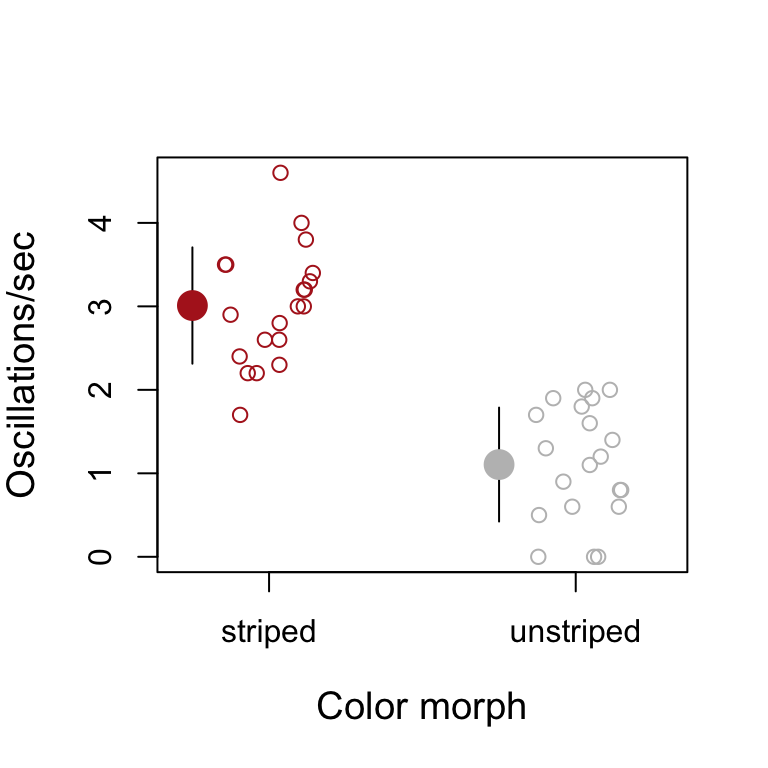
\includegraphics{Research-Design---Statistics_files/figure-latex/c3c86-1} \end{center}

Wow, things are getting complicated! Don't worry and don't feel overwhelmed. There is a learning curve to R, and I'm even including some quantitative metrics here that we won't cover in detail until later chapters. But let's break down what this strip chart is showing:

\begin{itemize}
\item
  Open circles: These represent the observed data points. These are added by the stripchart function. Note that I've color-coded each morph, which isn't completely necessary but can add a nice visual touch. Other new arguments here are \texttt{vertical}, which I've used to make the stripchart orient vertically, and \texttt{jitter}, which is used to add some random distance among the points along the x-axis. The jitter is useful to make points with very similar measurements more distinct.
\item
  Closed circles: These are the estimated means. Notice that I didn't simply use the mean function directly to quantify these. Because I wanted to estiamte the mean separately for each group, I had to use a new function: \texttt{aggregate}. The \texttt{aggregate} function allows you to compute a descriptive statistic separately by groups that you've defined, in this case the \textbf{morph}. Notice that I also computed the standard deviation by color morph with the aggregate function.
\end{itemize}

*Thin black lines: These are error bars representing one standard deviation away from the mean. Recall that the standard deviation is a descriptive metric of variation among individuals in a dataset.

So what does this graph tell us? Well, it tells us largely the same thing we saw with the box plots, except this time with all of the data visualized and with some different descriptive statistics. We can see that the standard deviation is very similar between color morphs, but the means appear to differ quite a bit.

Based on these graphs, can we conclude that the striped morphs have greater initial velocity in their autotomized tails than the unstriped morphs? You might be tempted to do so, but all we have done to this point is \emph{describe} the data. If you want to make a conclusion about whether something like the mean differs between groups, then you need different statistical tools, namely the tools of \textbf{inferential statistics}. Why? We'll discover the reasons in detail later in the book, but to hold you over, the main reason we can't make an inference about hte difference in means is because those means are \textbf{estimates}, and estimates have uncertainty. We need tools to examine that uncertainty before we can make any rigorous comparison of the mean between the groups of interest. More to come!

\subsection{Associations between qualitative variables}\label{associations-between-qualitative-variables}

Examining associations between categorical variables is even simpler in some ways. Let's consider another example from the squirrel dataset. Recall that squirrels were described by their primary fur color. Might behavior vary among individuals with different primary fur color? As just one example, for each squirrel in the dataset, the observer recorded whether or not the individual was climbing at the time it was observed. To examine the association, we can compute the proportion of squirrels observed climbining within each category of primary fur color:

\begin{Shaded}
\begin{Highlighting}[]
\DocumentationTok{\#\# quantify proportion climbing by fur color}
\NormalTok{p.climb }\OtherTok{\textless{}{-}} \FunctionTok{aggregate}\NormalTok{(climbing }\SpecialCharTok{\textasciitilde{}}\NormalTok{ primary.fur.color, }\AttributeTok{data =}\NormalTok{ sq, }\AttributeTok{FUN =}\NormalTok{ mean)}

\CommentTok{\# Plot}
\FunctionTok{barplot}\NormalTok{(}
  \AttributeTok{height =}\NormalTok{ p.climb}\SpecialCharTok{$}\NormalTok{climbing,}
  \AttributeTok{ylim=}\FunctionTok{c}\NormalTok{(}\DecValTok{0}\NormalTok{, }\FloatTok{0.25}\NormalTok{),}
  \AttributeTok{names.arg =}\NormalTok{ p.climb}\SpecialCharTok{$}\NormalTok{primary.fur.color,}
  \AttributeTok{xlab =} \StringTok{"Primary Fur Color"}\NormalTok{,}
  \AttributeTok{ylab =} \StringTok{"Proportion Climbing"}\NormalTok{,}
  \AttributeTok{col =} \FunctionTok{c}\NormalTok{(}\StringTok{"black"}\NormalTok{, }\StringTok{"brown"}\NormalTok{, }\StringTok{"gray"}\NormalTok{)}
\NormalTok{)}
\end{Highlighting}
\end{Shaded}

\begin{center}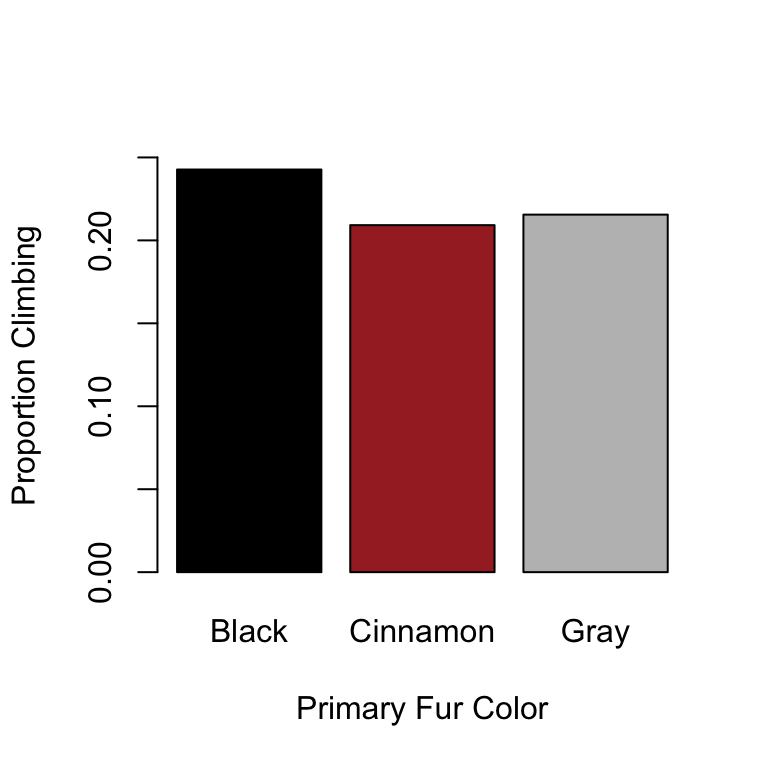
\includegraphics{Research-Design---Statistics_files/figure-latex/c3c87-1} \end{center}

Here I used the aggregate function again, this time to quantify the proportion climbing by categories of \texttt{primary.fur.color}. Notice that the function I used to quantify the proportion climbing within each category is the mean. Interesting! How does that work? Well, recall that climbing is defined as a logical variable, being TRUE for individuals who were observed climbing, and FALSE for those that weren't climbing. When a mathematical function is applied to a logic variable, R treats the variable as a binary numeric variable with values of 0 and 1. The TRUE observations are defined as 1, and the FALSE observations are defined as 0. Suppose we five observations of climbing were \{TRUE, FALSE, FALSE, TRUE, FALSE\}. If I quantify the mean of that variable, R converts the variable to \{1, 0, 0, 1, 0\}, and then quantifies the mean as

\[
\hat{\mu} = \frac{1 + 0 + 0 + 1 + 0}{5}=0.4
\]

The mean of a binary variable with values of 0 and 1s is the same as the proportion:

\[
\hat{p}_{\text{climbing}} = \frac{2}{5} = 0.4
\]

Cool!

Now, all we've done here is describe the observed data. Is the probability of climbing different among the categories of primary fur color? Our descriptive estimates of the proportion climbing are definitely different, but remember this is only a description of estimates that have uncertainty. We need to examine that uncertainty to inform our conclusion about whether climbing behavior really differs among these groups. Stay tuned!

\section{Some final points about R}\label{some-final-points-about-r}

\subsection{Packages}\label{packages}

All of the R code that we executed in R was done with the basic functionality that comes with R when first installed. But one of the best things about R is that anyone can write their own functions and share them with others via packages. For example, all of the plots that I created above were created with base R functions, but there are many other packages that others have developed that can be used to create plots. One of the most popular of those packages is called \texttt{ggplot2}, so let's take a look at it.

\subsection{Installing a package}\label{installing-a-package}

When you want to use functions from a specialized package in R, you first have to install the package with those functions. You can install packages with the \texttt{install.packages} function. The main argument of the \texttt{install.packages} function is a character vector of the packages you want to install. If you only want to install a single package, just write the name of the package as a character:

\begin{Shaded}
\begin{Highlighting}[]
\FunctionTok{install.packages}\NormalTok{(}\StringTok{"ggplot2"}\NormalTok{)}
\end{Highlighting}
\end{Shaded}

\begin{verbatim}
## Error in install.packages : Updating loaded packages
\end{verbatim}

When you execute the code, you'll see R will download the package and install it.

\subsection{Using functions from a package}\label{using-functions-from-a-package}

After you've installed a package, you can start to use functions from the package, but to do so, you have to tell R you want to use the functions in that package. One way to do this is to load the package with the \texttt{library} function:

\begin{Shaded}
\begin{Highlighting}[]
\FunctionTok{library}\NormalTok{(ggplot2)}
\end{Highlighting}
\end{Shaded}

Once you execute the code to load the package, you can then use any function in the package just as you'd use functions from base R. For example, we can use the ggplot function to create the scatterplot we created above relating the length and mass of salamanders:

\begin{Shaded}
\begin{Highlighting}[]
\FunctionTok{ggplot}\NormalTok{(tail, }\FunctionTok{aes}\NormalTok{(}\AttributeTok{x =}\NormalTok{ length.cm, }\AttributeTok{y =}\NormalTok{ mass.g)) }\SpecialCharTok{+}
  \FunctionTok{geom\_point}\NormalTok{(}\AttributeTok{shape =} \DecValTok{19}\NormalTok{) }\SpecialCharTok{+}
  \FunctionTok{labs}\NormalTok{(}\AttributeTok{x =} \StringTok{"Snout{-}vent length (cm)"}\NormalTok{, }\AttributeTok{y =} \StringTok{"Mass (g)"}\NormalTok{, }\AttributeTok{title =} \StringTok{""}\NormalTok{)}
\end{Highlighting}
\end{Shaded}

\begin{center}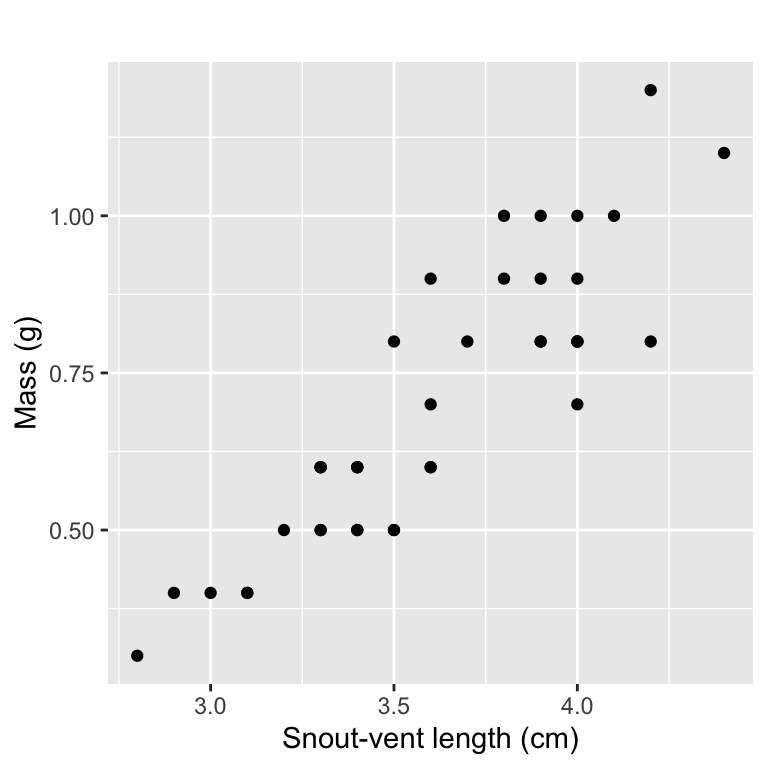
\includegraphics{Research-Design---Statistics_files/figure-latex/c3c90-1} \end{center}

The ggplot function has it's own quirks, one of which is that it works with a hierarchical set of functions. Most directly we specified that a plot will be created with the tail data frame, but then we used the \texttt{aes} function from ggplot to describe which variables in the tail data frame should be associated, in this case placing mass on the y-axis and length on the x-axis. But additional components need to be specified with susbequent functions, called ``layers''. Different layers are added to the graph using the layer operator, \texttt{+}. To improve readability, the \texttt{+} operator is often placed at the end of each line when breaking up commands across multiple lines.

Let me show you what I mean. Suppose I only executed the first line of code without the layer operator and subsequeent layers. Let's do that and see what the plot looks like:

\begin{Shaded}
\begin{Highlighting}[]
\FunctionTok{ggplot}\NormalTok{(tail, }\FunctionTok{aes}\NormalTok{(}\AttributeTok{x =}\NormalTok{ length.cm, }\AttributeTok{y =}\NormalTok{ mass.g))}
\end{Highlighting}
\end{Shaded}

\begin{center}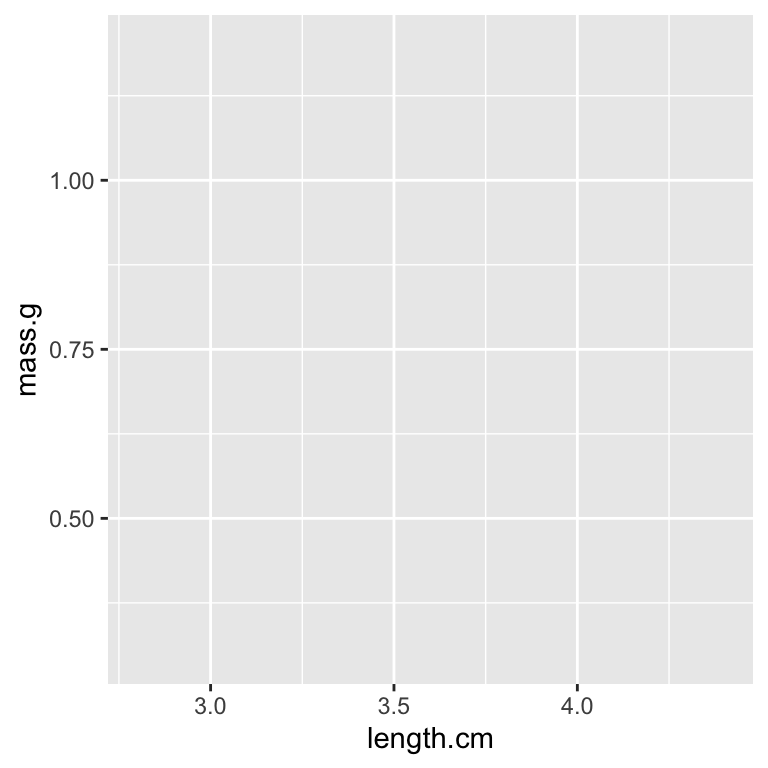
\includegraphics{Research-Design---Statistics_files/figure-latex/c3c91-1} \end{center}

It's incompelte. It put the names of the vector I wanted on the x- and y-axes, but it didn't plot any points. The points get plotted with the \texttt{geom\_point} layer, specifying the points with shape = 19, which is simply a closed circle:

\begin{Shaded}
\begin{Highlighting}[]
\FunctionTok{ggplot}\NormalTok{(tail, }\FunctionTok{aes}\NormalTok{(}\AttributeTok{x =}\NormalTok{ length.cm, }\AttributeTok{y =}\NormalTok{ mass.g)) }\SpecialCharTok{+}
  \FunctionTok{geom\_point}\NormalTok{(}\AttributeTok{shape =} \DecValTok{19}\NormalTok{) }
\end{Highlighting}
\end{Shaded}

\begin{center}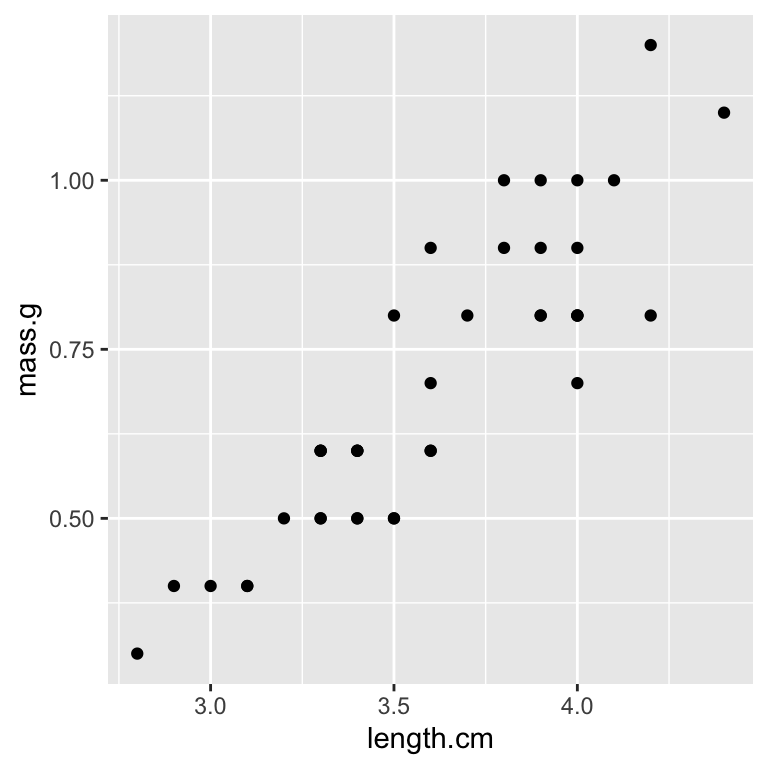
\includegraphics{Research-Design---Statistics_files/figure-latex/c3c92-1} \end{center}

Now we see the points, but to label the x- and y-axes correctly, you have to add another layer via the \texttt{labs} function.

\begin{Shaded}
\begin{Highlighting}[]
\FunctionTok{ggplot}\NormalTok{(tail, }\FunctionTok{aes}\NormalTok{(}\AttributeTok{x =}\NormalTok{ length.cm, }\AttributeTok{y =}\NormalTok{ mass.g)) }\SpecialCharTok{+}
  \FunctionTok{geom\_point}\NormalTok{(}\AttributeTok{shape =} \DecValTok{19}\NormalTok{) }\SpecialCharTok{+}
  \FunctionTok{labs}\NormalTok{(}\AttributeTok{x =} \StringTok{"Snout{-}vent length (cm)"}\NormalTok{, }\AttributeTok{y =} \StringTok{"Mass (g)"}\NormalTok{, }\AttributeTok{title =} \StringTok{""}\NormalTok{)}
\end{Highlighting}
\end{Shaded}

\begin{center}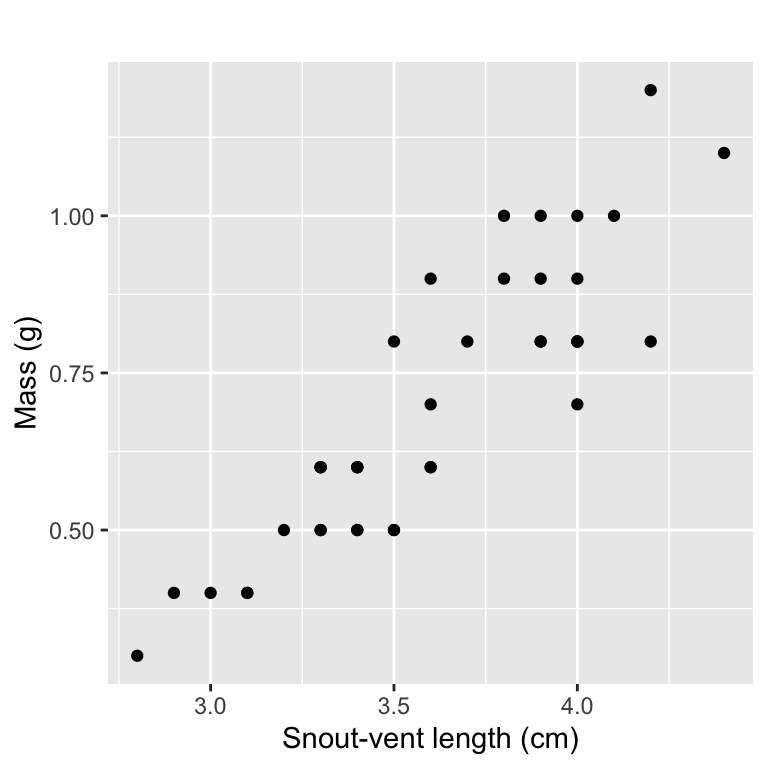
\includegraphics{Research-Design---Statistics_files/figure-latex/c3c93-1} \end{center}

All of the types of graphs I created above could be created with ggplot2. For example:

\begin{Shaded}
\begin{Highlighting}[]
\FunctionTok{ggplot}\NormalTok{(tail, }\FunctionTok{aes}\NormalTok{(}\AttributeTok{x =}\NormalTok{ tail.vel)) }\SpecialCharTok{+}
  \FunctionTok{geom\_histogram}\NormalTok{(}\AttributeTok{binwidth =} \FloatTok{0.5}\NormalTok{, }\AttributeTok{color =} \StringTok{"black"}\NormalTok{, }\AttributeTok{fill =} \StringTok{"lightblue"}\NormalTok{) }\SpecialCharTok{+} 
  \FunctionTok{labs}\NormalTok{(}\AttributeTok{x =} \StringTok{"Initial velocity (oscillations/sec)"}\NormalTok{, }\AttributeTok{y =} \StringTok{"Number of individuals"}\NormalTok{)}
\end{Highlighting}
\end{Shaded}

\begin{center}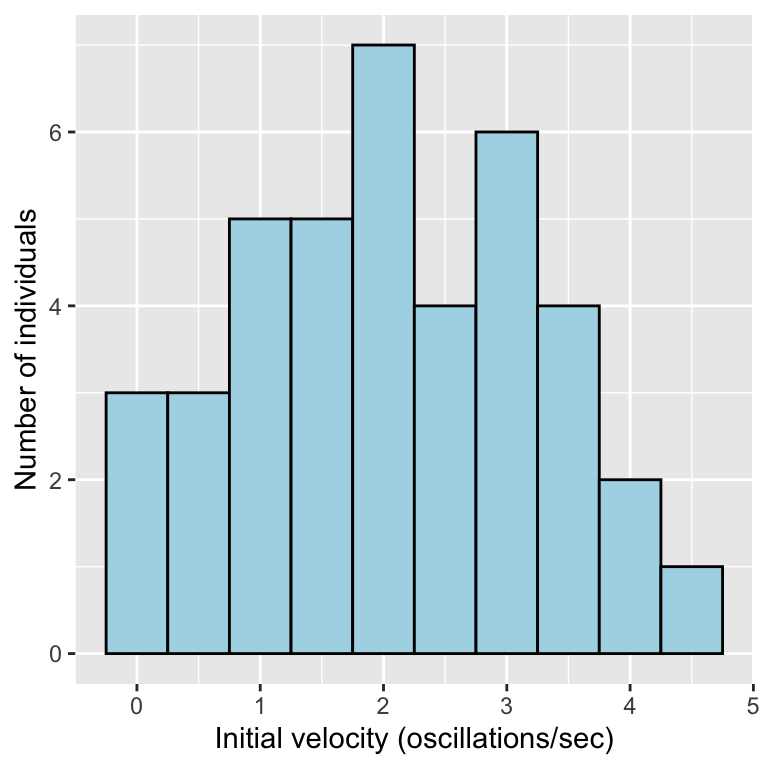
\includegraphics{Research-Design---Statistics_files/figure-latex/c3c94-1} \end{center}

\begin{Shaded}
\begin{Highlighting}[]
\FunctionTok{ggplot}\NormalTok{(tail, }\FunctionTok{aes}\NormalTok{(}\AttributeTok{x =} \StringTok{""}\NormalTok{, }\AttributeTok{y =}\NormalTok{ tail.vel)) }\SpecialCharTok{+}
  \FunctionTok{geom\_boxplot}\NormalTok{() }\SpecialCharTok{+}
  \FunctionTok{labs}\NormalTok{(}\AttributeTok{x =} \StringTok{"Initial velocity"}\NormalTok{, }\AttributeTok{y =} \StringTok{"Oscillations/sec"}\NormalTok{)}
\end{Highlighting}
\end{Shaded}

\begin{center}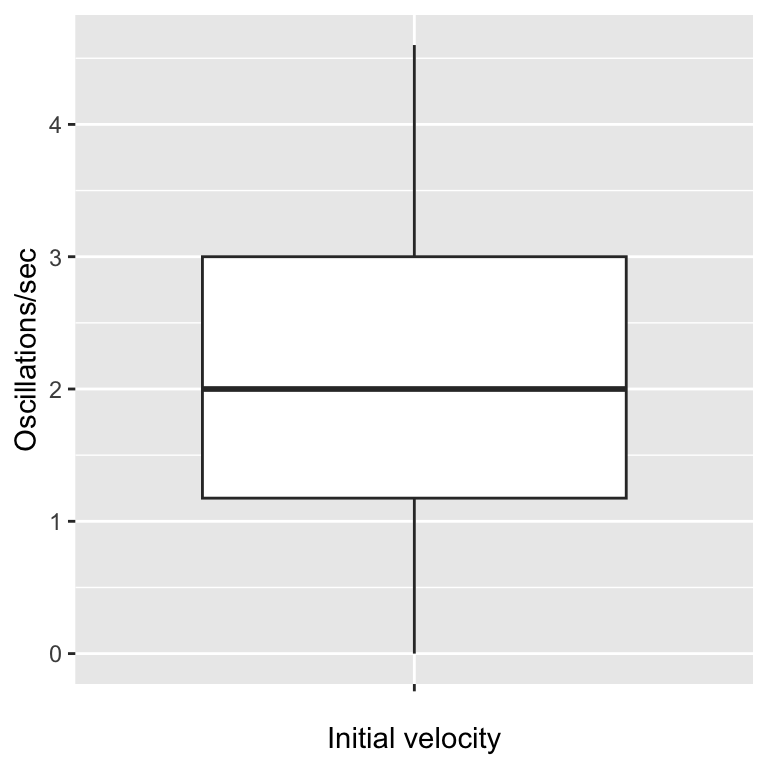
\includegraphics{Research-Design---Statistics_files/figure-latex/c3c94-2} \end{center}

\begin{Shaded}
\begin{Highlighting}[]
\FunctionTok{ggplot}\NormalTok{(tail, }\FunctionTok{aes}\NormalTok{(}\AttributeTok{x =} \StringTok{""}\NormalTok{, }\AttributeTok{y =}\NormalTok{ tail.vel)) }\SpecialCharTok{+}
  \FunctionTok{geom\_jitter}\NormalTok{(}\AttributeTok{width =} \FloatTok{0.2}\NormalTok{, }\AttributeTok{shape =} \DecValTok{1}\NormalTok{) }\SpecialCharTok{+} 
  \FunctionTok{labs}\NormalTok{(}\AttributeTok{x =} \StringTok{"Initial velocity"}\NormalTok{, }\AttributeTok{y =} \StringTok{"Oscillations/sec"}\NormalTok{)}
\end{Highlighting}
\end{Shaded}

\begin{center}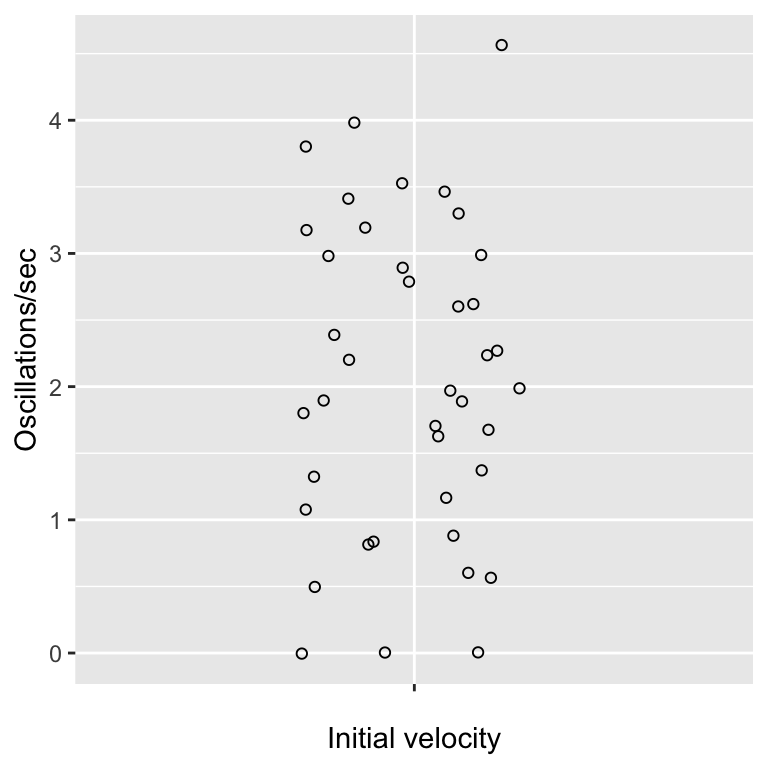
\includegraphics{Research-Design---Statistics_files/figure-latex/c3c94-3} \end{center}

\subsection{Scripting}\label{scripting}

One last R skill that I'd like to briefly cover is scripting. Doing analysis by coding is great for a variety of reasons, but one of the best reasons to code is to make your science reproducible with a script. When you execute a set o functions for an analysis, you can save the code to execute those functions in a script, which is basically a text file (with an .R extension).

Suppose you're working on an analysis for an hour and then the power goes out. Well, if you were scripting your analysis, all you have to do is load your script and execute all the functions up to the point where you left off. A script allows you go back and easily make changes, and it allows others to see \emph{exactly} how you performed an analysis. Indeed, most scientific journals are now requiring that authors publish their code used to conduct analyses to be completely transparent about how the analyses were performed.

How do you make a script? It's really easy in RStudio? In your toolbar, just click File, New File, and then R script. That will open a text editor in the top left panel of RStudio. From there you can start writing your code. I strongly recommend that you add notes to your code to describe what the code is doing. These notes don't have to be extensive, but it's very useful to help reorient yourself, or orient someone else for the first time, to what the code is doing.

For example, Figure \ref{fig:c3f4} shows a simple script that I wrote to perform some basic descriptive statistics on the salamander tails data. I included some notes to delineate different sections of the script. The dashes are not necessary, but I often use them because they allow me to visually demarcate the different sections of the script, and RStudio recognizes those sections and allows you to navigate among the different sections using the drop-down in the bottom left corner of the script panel.

\begin{figure}
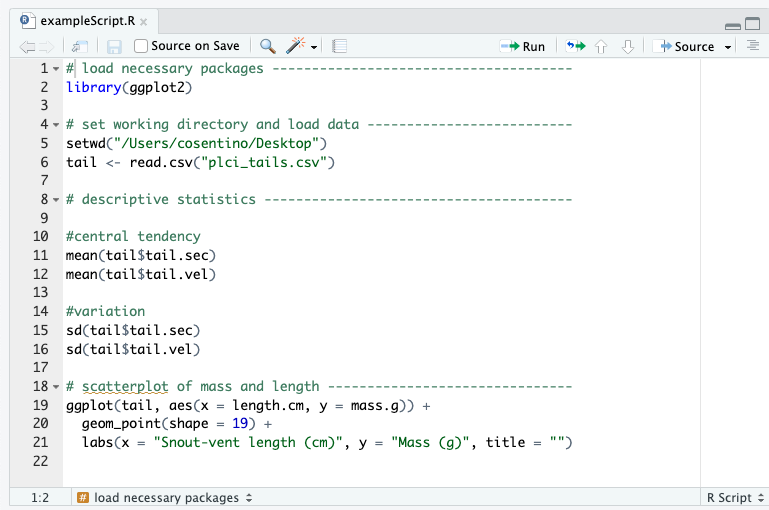
\includegraphics[width=0.9\linewidth]{images/03_exampleScript} \caption{Unstriped (left) and striped color morphs of red-backed salamanders.}\label{fig:c3f4}
\end{figure}

How do you execute the code in a script? It's easy! Just highlight the code that you want to execute, then click the ``Run'' button in the top right corner of the script panel. You'll see the code executed in the R console in the bottom left panel, along with any generated output.

\chapter{Graphical Causal Models}\label{graphical-causal-models}

I've made the case that science starts with a clear research question, and we've explored some characteristics of what defines a good research question. I've also suggested that many (maybe most) scientific research studies have a primary goal of testing a causal hypothesis. In this chapter, we will take a closer look at causal questions. Designing scientific studies to address causal questions can be extremely challenging. Overcoming those challenges requires a clearly stated scientific model of the causal effects being hypothesized. Describing your scientific model and stating your causal assumptions with a graph is the focus of this chapter, and a theme that we will come back to as we explore the particulars of research design and statistics in the remainder of the book.

\section{Directed acyclic graphs (DAGs)}\label{directed-acyclic-graphs-dags}

There are two general approaches to \textbf{causal inference}: the potential outcomes framework (\href{https://www.jstor.org/stable/2245382}{Neyman 1923}, \href{https://www.jstor.org/stable/27590541}{Rubin 2005}) and the graphical causal model framework (\href{https://bayes.cs.ucla.edu/BOOK-2K/}{Pearl 2000}). In this book, we will use graphical causal models to guide our approach to causal inference. I find that the graphical representation of causal models provides for a smoother entry to the ideas of causal inference for students in an introductory statistics course.

The graphical causal modeling framework uses \textbf{directed acyclic graphs (DAGs)} to visualize the causal assumptions of a hypothesis. Let's work through an example. Suppose you are interested in the causal effect of living near urban greenspace on mental health. In cities, greenspaces are simply areas where natural vegetation occurs, such as forest. This is a forward causal question with a clearly defined cause (greenspace) and effect (mental health). The hypothesis is that living near greenspace reduces the risk of mental health disorders, perhaps by alleviating anxiety, or encouraging physical activity. Causal effects of one variable on another can involve multiple mechanisms.

Let's assume that we can measure whether or not people live near greenspace. We define \texttt{greenspace} as a nominal variable where individuals live either ``near greenspace'' or ``not near greenspace''. In reality, proximity to greenspace can be measured on a continuum, but for now let's keep it simple and define proximity categorically. Let's also assume that \texttt{mental.health} is a binary, categorical variable. People either have a mental health disorder, or they don't.

Our causal hypothesis is represented as a DAG in Figure \ref{fig:c4c1}. This kind of graph has nodes that represent variables, and arrows between nodes that illustrate the flow of causation. Based on how we've talked about our research question to this point, we have a really simple DAG. The nodes are greenspace and mental health, and there's a directional arrow from greenspace to mental health. The direction of the arrow shows the direction of causality. This DAG implies that greenspace directly influences mental health. Because there are no other variables between these variables, we define the effect of greenspace on mental health as a \textbf{direct effect}.

\begin{Shaded}
\begin{Highlighting}[]
\FunctionTok{library}\NormalTok{(dagitty)}
\FunctionTok{library}\NormalTok{(rethinking)}
\NormalTok{dag1 }\OtherTok{\textless{}{-}} \FunctionTok{dagitty}\NormalTok{(}\StringTok{"dag \{greenspace {-}\textgreater{} mental.health\}"}\NormalTok{)}
\FunctionTok{coordinates}\NormalTok{(dag1) }\OtherTok{\textless{}{-}} \FunctionTok{list}\NormalTok{(}\AttributeTok{x =} \FunctionTok{c}\NormalTok{(}\AttributeTok{greenspace =} \DecValTok{0}\NormalTok{, }\AttributeTok{mental.health =} \DecValTok{1}\NormalTok{), }\AttributeTok{y =} \FunctionTok{c}\NormalTok{(}\AttributeTok{greenspace =} \DecValTok{0}\NormalTok{, }\AttributeTok{mental.health =} \DecValTok{0}\NormalTok{))}
\FunctionTok{drawdag}\NormalTok{(dag1)}
\end{Highlighting}
\end{Shaded}

\begin{figure}

{\centering 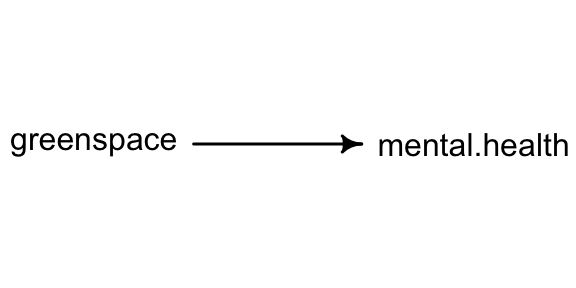
\includegraphics{Research-Design---Statistics_files/figure-latex/c4c1-1} 

}

\caption{Initial DAG for the causal effect of greenspace on mental health.}\label{fig:c4c1}
\end{figure}

Our hypothesis is that greenspace \emph{reduces} the risk of mental health disorders, but note there's no indication of the nature of the causal effect in the DAG. DAGs simply illustrate assumed causal effects. DAGs do not assume anything about the form of the causal relationship between variables (e.g., positive vs.~negative relationship, linear vs.~non-linear relationship).

Drawing DAGs

In this chapter and throughout the book I will create figures of DAGs in R with the \texttt{dagitty} and \texttt{rethinking} packages. The relationship between variables are defined by the \texttt{dagitty} function, with the arrow \texttt{-\textgreater{}} identifying the direction of causality between variables. You can use the \texttt{coordinates} function to customize the arrnangement of the variables in the plot along x- and y-axes.

I also highly recommend the \href{https://www.dagitty.net/}{dagitty website}, where you can draw DAGs directly in your internet browser.

Life is rarely so simple as assumed in our initial DAG. Notably, the DAG assumes that greenspace is the only significant cause of mental health. The emphasis on significant is purposeful. In reality, there may be hundreds of causes of mental health. Most outcomes in biology are like this with multiple possible causes. However, DAGs focus on the most important causes. If there's a particular mutation on a gene that increases the risk of a mental health disorder by 0.001\%, we probably don't need to include that in the DAG because the effect is trivial. Additionally, because we are focusing on mental health as an outcome, we don't necessarily need to include variables that are causally affected by mental health. Overall, some discretion about the variables to include in DAGs is warranted, because otherwise DAGs would be too complex to be useful (\href{https://theeffectbook.net/}{Huntington-Klein 2022}). All models are simplifications.

Suppose that we collect some idea, and we find that 18\% of individuals who don't live near greenspace have been diagnosed with a mental health disorder, whereas 11\% of individuals who live near greenspace have a mental health disorder. The absolute risk \footnote{\textbf{Absolute risk} is the probability that an event occurs, here expressed as a percentage. Absolute risk can be contrasted with \textbf{relative risk}, which is the proportional risk of one outcome relative to another. For example, if the absolute risk of a mental health disorder is 18\% for the ``near greenspace'' group and 11\% for the ``not near greenspace'' group, then the relative risk of living near greenspace is 0.11/0.18 = 0.61. This means that it is 0.61 times less likely to be diagnosed with a mental health disorder when living near greenspace relative to not living near greenspace. Relative risk and absolute risk are often reported in the medical literature, but note that relative risk doesn't tell you anything about the absolute risk. One useful way of comparing risk between groups on the absolute risk scale is the \textbf{absolute risk reduction}, which just the difference in absolute risk between groups. That's the 7\% that I referenced in the text.} of a mental health disorder is 7\% lower for individuals who live near greenspace. Is that difference caused by greenspace? Not necessarily! Why not? We need to consider the possibility that there is a common cause of greenspace and mental health. In other words, the people who live near greenspace differ in other ways from the people who don't live near greenspace, and these differences might contribute to mental health outcomes. One such possibility is socioeconomic status (SES). SES is very likely a cause of living near greenspace because wealthy people can afford to live near greenspace. SES might also be a cause of mental health because wealthy people have good access to healthcare. Figure \ref{fig:c4c2} adds SES to the DAG.

\begin{Shaded}
\begin{Highlighting}[]
\NormalTok{dag2 }\OtherTok{\textless{}{-}} \FunctionTok{dagitty}\NormalTok{(}\StringTok{"dag \{greenspace {-}\textgreater{} mental.health;}
\StringTok{                      SES {-}\textgreater{} greenspace;}
\StringTok{                      SES {-}\textgreater{} mental.health\}"}\NormalTok{)}
\FunctionTok{coordinates}\NormalTok{(dag2) }\OtherTok{\textless{}{-}} \FunctionTok{list}\NormalTok{(}\AttributeTok{x =} \FunctionTok{c}\NormalTok{(}\AttributeTok{greenspace =} \DecValTok{0}\NormalTok{, }\AttributeTok{SES =} \DecValTok{1}\NormalTok{, }\AttributeTok{mental.health =} \DecValTok{2}\NormalTok{), }
                          \AttributeTok{y =} \FunctionTok{c}\NormalTok{(}\AttributeTok{greenspace =} \DecValTok{0}\NormalTok{, }\AttributeTok{SES =} \SpecialCharTok{{-}}\DecValTok{1}\NormalTok{, }\AttributeTok{mental.health =} \DecValTok{0}\NormalTok{))}
\FunctionTok{drawdag}\NormalTok{(dag2)}
\end{Highlighting}
\end{Shaded}

\begin{figure}

{\centering 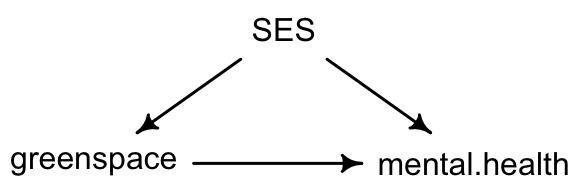
\includegraphics{Research-Design---Statistics_files/figure-latex/c4c2-1} 

}

\caption{DAG with the confounding variable SES added.}\label{fig:c4c2}
\end{figure}

The new DAG in Figure \ref{fig:c4c2} clearly identifies SES as a common cause of both greenspace and mental health. This means the causal relationship between greenspace and mental health is confounded by SES. We call SES a \textbf{confounding variable} because it affects both the explanatory and response variables, ultimately confusing our interpretation of the relationship between greenspace and mental health. Remember that the risk of having a mental health disorder was 7\% lower for people who live close to greenspace. It's possible that difference is due to a causal effect of greenspace on mental health, but it's also possible that some or all of the risk difference is due to the confounding effect of SES. Confounding variables can create associations between variables that are not causal.

Let me show you what I mean with the help of a data simulation. The risk probabilities of having a mental health disorder that I previously mentioned were generated by simulating data in R. Here's the code, followed by an explanation:

\begin{Shaded}
\begin{Highlighting}[]
\FunctionTok{set.seed}\NormalTok{(}\DecValTok{122}\NormalTok{)}

\DocumentationTok{\#\# simulate socioeconomic status (ses)}
\NormalTok{ses }\OtherTok{\textless{}{-}} \FunctionTok{rbinom}\NormalTok{(}\AttributeTok{n =} \DecValTok{1000}\NormalTok{, }\AttributeTok{size =} \DecValTok{1}\NormalTok{, }\AttributeTok{prob =} \FloatTok{0.5}\NormalTok{)}

\DocumentationTok{\#\# simulate green space access (grn) based on ses}
\NormalTok{grn }\OtherTok{\textless{}{-}} \FunctionTok{rbinom}\NormalTok{(}\AttributeTok{n =} \DecValTok{1000}\NormalTok{, }\AttributeTok{size =} \DecValTok{1}\NormalTok{, }\AttributeTok{prob =} \FunctionTok{ifelse}\NormalTok{(ses }\SpecialCharTok{==} \DecValTok{1}\NormalTok{, }\FloatTok{0.8}\NormalTok{, }\FloatTok{0.2}\NormalTok{))}

\DocumentationTok{\#\# simulate mental health status (mnt) based on ses}
\NormalTok{mnt }\OtherTok{\textless{}{-}} \FunctionTok{rbinom}\NormalTok{(}\AttributeTok{n =} \DecValTok{1000}\NormalTok{, }\AttributeTok{size =} \DecValTok{1}\NormalTok{, }\AttributeTok{prob =} \FunctionTok{ifelse}\NormalTok{(ses }\SpecialCharTok{==} \DecValTok{1}\NormalTok{, }\FloatTok{0.1}\NormalTok{, }\FloatTok{0.2}\NormalTok{))}
\end{Highlighting}
\end{Shaded}

I assumed that we have a dataset of \(n = 1000\) people, and for each person, I first randomly determined if they are of high or low socioeconomic status. I did this using a function called \texttt{rbinom}. The arguments of the \texttt{rbinom} function include the number of observations (\texttt{n\ =\ 1000}), the number of trials (\texttt{size\ =\ 1}), and the probability of ``success'' (\texttt{prob\ =\ 0.5}). What this means is that for each of the 1000 individuals, I determine a single time whether they are of high or low SES, each with a probability of 0.5. This produces the variable \texttt{ses}, a vector of 0 and 1 values, where 0 represents ``low ses'' and 1 represents ``high ses''. Because I set the probability of success to 0.5, there should be about a 50/50 split of low and high ses individuals. It won't necessarily be exactly 50\%, because the function is drawing values randomly. It's basically like flipping a coin 1000 times and counting heads and tails.

Once the ses variable was generated, I then generated the greenspace access variable, called \texttt{grn}. This was also generated with the \texttt{rbinom} function, where a 1 represents ``near greenspace'' and 0 represents ``not near greenspace''. I used the \texttt{ifelse} function to specify that the probability of being near greenspace was 0.8 for individuals of high ses and 0.2 for individuals of low ses. Finally, I generated a variable for mental health outcome, \texttt{mnt}, where 1 represents individuals who have a mental health disorder, and 0 represents individuals who don't have a mental health disorder. I assumed the probability of a mental health disorder was 0.1 for individuals of high ses and 0.2 for individuals of low ses. The only other part of the code chunk above is the \texttt{setseed} function, which allows you to simulate the exact same dataset that I simulated, as long as you use the same \texttt{setseed} number (122).

Now I want you to notice something important. Because we are simulating data, I had to make some assumptions about what the probability of a mental health disorder would be for individuals of high and low ses and individuals who are near or not near greenspace. In this simulation, I assumed that mental health risk is \emph{only} affected by SES. There is no direct effect of greenspace access on mental health risk based in this simulation. Let's see what happens when we compare the probability of a mental health disorder between greenspace access based on this simulated dataset. We can do that with the \texttt{table} function:

\begin{Shaded}
\begin{Highlighting}[]
\FunctionTok{table}\NormalTok{(mnt, grn)}
\end{Highlighting}
\end{Shaded}

\begin{verbatim}
##    grn
## mnt   0   1
##   0 421 436
##   1  90  53
\end{verbatim}

Here we see a \textbf{contingency table} showing the number of individuals in each category of mental health status and greenspace. Greenspace, the explanatory variable, is located at the top of the table, where the column for \texttt{grn} = 0 represents not near greenspace, and the column for \texttt{grn} = 1 represents individuals who live near greenspace. The rows represent the categories of mental health status, where \texttt{mnt} = 0 are the individuals who don't have a mental health disorder, and \texttt{mnt} = 1 are the individuals who have a mental health disorder. You can determine the totals in each category manually, or you can wrap the table function in a function called \texttt{addmargins}:

\begin{Shaded}
\begin{Highlighting}[]
\FunctionTok{addmargins}\NormalTok{(}\FunctionTok{table}\NormalTok{(mnt, grn))}
\end{Highlighting}
\end{Shaded}

\begin{verbatim}
##      grn
## mnt      0    1  Sum
##   0    421  436  857
##   1     90   53  143
##   Sum  511  489 1000
\end{verbatim}

With the addmargins function, we can see there were 511 people who don't live near greenspace and 489 people who do live near greenspace. We can also see the totals for mental health disorders: 143 people out of the 1000 have a mental health disorder. With this information, we can now compute the probability of a mental health disorder for the two categories of greenspace. This is exactly what a researcher might be tempted to do to assess whether living near greenspace causally affect mental health risk:

\begin{Shaded}
\begin{Highlighting}[]
\NormalTok{p.mnt.g0 }\OtherTok{\textless{}{-}} \DecValTok{90}\SpecialCharTok{/}\DecValTok{511} \CommentTok{\#mental health risk when greenspace = 0}
\NormalTok{p.mnt.g0}
\end{Highlighting}
\end{Shaded}

\begin{verbatim}
## [1] 0.1761252
\end{verbatim}

\begin{Shaded}
\begin{Highlighting}[]
\NormalTok{p.mnt.g1 }\OtherTok{\textless{}{-}} \DecValTok{53}\SpecialCharTok{/}\DecValTok{489} \CommentTok{\#mental health risk when greenspace = 1}
\NormalTok{p.mnt.g1}
\end{Highlighting}
\end{Shaded}

\begin{verbatim}
## [1] 0.1083845
\end{verbatim}

So we see exactly what I told you earlier. Of the 1000 people in the dataset, 18\% of people not near greenspace had a mental health disorder, and 11\% of people near greenspace had a mental health disorder (I'm rounding to two decimal places). One might be tempted to infer that the causal effect of greenspace is the 7\% difference between these probabilities. But it's not! I know it's not, \textbf{because I simulated the data under the assumption greenspace access has no effect on mental health risk}. The only effect on mental health risk was SES. So why is there a 7\% difference in risk probability with respect to greenspace? That difference is driven entirely by the confounding effect of SES in this simulation. High SES increases the chance that an individual lives near greenspace, and high SES decreases the chance of a mental health disorder. We can see this in the data:

\begin{Shaded}
\begin{Highlighting}[]
\FunctionTok{addmargins}\NormalTok{(}\FunctionTok{table}\NormalTok{(grn, ses))}
\end{Highlighting}
\end{Shaded}

\begin{verbatim}
##      ses
## grn      0    1  Sum
##   0    393  118  511
##   1     81  408  489
##   Sum  474  526 1000
\end{verbatim}

\begin{Shaded}
\begin{Highlighting}[]
\DecValTok{81}\SpecialCharTok{/}\DecValTok{474} \CommentTok{\#probability of near greenspace when ses is low}
\end{Highlighting}
\end{Shaded}

\begin{verbatim}
## [1] 0.1708861
\end{verbatim}

\begin{Shaded}
\begin{Highlighting}[]
\DecValTok{408}\SpecialCharTok{/}\DecValTok{526} \CommentTok{\#probability of near greenspace when ses is high}
\end{Highlighting}
\end{Shaded}

\begin{verbatim}
## [1] 0.7756654
\end{verbatim}

\begin{Shaded}
\begin{Highlighting}[]
\FunctionTok{addmargins}\NormalTok{(}\FunctionTok{table}\NormalTok{(mnt,ses))}
\end{Highlighting}
\end{Shaded}

\begin{verbatim}
##      ses
## mnt      0    1  Sum
##   0    376  481  857
##   1     98   45  143
##   Sum  474  526 1000
\end{verbatim}

\begin{Shaded}
\begin{Highlighting}[]
\DecValTok{98}\SpecialCharTok{/}\DecValTok{474} \CommentTok{\#mental health risk when ses is low}
\end{Highlighting}
\end{Shaded}

\begin{verbatim}
## [1] 0.2067511
\end{verbatim}

\begin{Shaded}
\begin{Highlighting}[]
\DecValTok{45}\SpecialCharTok{/}\DecValTok{526} \CommentTok{\#mental health risk when ses is high}
\end{Highlighting}
\end{Shaded}

\begin{verbatim}
## [1] 0.08555133
\end{verbatim}

Here we see that the probability of living near greenspace was 17\% for low SES and 78\% for high SES, and the probability of a mental health disorder was 21\% for low SES and 9\% for high SES. In this dataset, the people of low SES with a greater risk of a mental health disorder also tend to not live near greenspace.

OK - Who cares? Well, if you want to design a study to investigate whether or not greenspace has a causal effect on mental health, you'd get the wrong answer if you simply compared the raw risk of mental health disorders between people who do and do not live near greenspace. The DAG makes this clear, identifying SES as a confounding variable. If you want to get the right answer, the DAG shows us that we need to take into consideration the socioeconomic status of people. If we don't take SES into consideration, then the relationship we observe between greenspace and mental health will include a mix of the real causal effect of greenspace on mental health \emph{and} the noncausal association via SES. \textbf{\emph{DAGs make our causal assumptions clear and inform how we should design a study and conduct analyses to isolate the causal effects of interest}}.

Later in the book we will learn more about what it means to take a variable ``into consideration'' when estimating a causal effect of some other variable, but let me briefly show you with this example. Basically, we need to look at the relationship between greenspace and mental health risk \emph{while holding SES constant}. In other words, we need to compare the mental health risk between greenspace levels within the different categories of SES. Let's do this and see what we find. First, let's combine our variables into a dataframe, and then subset the dataset into two datasets, one for people of low SES, and another for people of high SES:

\begin{Shaded}
\begin{Highlighting}[]
\NormalTok{d }\OtherTok{\textless{}{-}} \FunctionTok{cbind.data.frame}\NormalTok{(ses, grn, mnt) }\CommentTok{\#create a data frame with all 3 variables}
\NormalTok{lo.ses }\OtherTok{\textless{}{-}}\NormalTok{ d[d}\SpecialCharTok{$}\NormalTok{ses }\SpecialCharTok{==} \DecValTok{0}\NormalTok{,]}
\NormalTok{hi.ses }\OtherTok{\textless{}{-}}\NormalTok{ d[d}\SpecialCharTok{$}\NormalTok{ses }\SpecialCharTok{==} \DecValTok{1}\NormalTok{,]}
\end{Highlighting}
\end{Shaded}

Now, let's compare the mental health risk between greenspace levels within each dataset. First, the individuals of low SES:

\begin{Shaded}
\begin{Highlighting}[]
\FunctionTok{addmargins}\NormalTok{(}\FunctionTok{table}\NormalTok{(lo.ses}\SpecialCharTok{$}\NormalTok{mnt, lo.ses}\SpecialCharTok{$}\NormalTok{grn,}
                 \AttributeTok{dnn=}\FunctionTok{c}\NormalTok{(}\StringTok{"mnt"}\NormalTok{, }\StringTok{"grn"}\NormalTok{))) }\CommentTok{\#dnn argument adds names to the table}
\end{Highlighting}
\end{Shaded}

\begin{verbatim}
##      grn
## mnt     0   1 Sum
##   0   310  66 376
##   1    83  15  98
##   Sum 393  81 474
\end{verbatim}

\begin{Shaded}
\begin{Highlighting}[]
\DecValTok{83}\SpecialCharTok{/}\DecValTok{393} \CommentTok{\#mental health risk for not near greenspace}
\end{Highlighting}
\end{Shaded}

\begin{verbatim}
## [1] 0.2111959
\end{verbatim}

\begin{Shaded}
\begin{Highlighting}[]
\DecValTok{15}\SpecialCharTok{/}\DecValTok{81} \CommentTok{\#mental health risk for near greenspace}
\end{Highlighting}
\end{Shaded}

\begin{verbatim}
## [1] 0.1851852
\end{verbatim}

Here we see a less than 3\% difference in mental health risk between the levels of greenspace access. We'll learn that the difference we observe here is not a real causal effect; rather it's due entirely to what we'll call \textbf{sampling error}. More on that later.

How about the individuals of high SES?

\begin{Shaded}
\begin{Highlighting}[]
\FunctionTok{addmargins}\NormalTok{(}\FunctionTok{table}\NormalTok{(hi.ses}\SpecialCharTok{$}\NormalTok{mnt, hi.ses}\SpecialCharTok{$}\NormalTok{grn,}
                 \AttributeTok{dnn=}\FunctionTok{c}\NormalTok{(}\StringTok{"mnt"}\NormalTok{, }\StringTok{"grn"}\NormalTok{))) }
\end{Highlighting}
\end{Shaded}

\begin{verbatim}
##      grn
## mnt     0   1 Sum
##   0   111 370 481
##   1     7  38  45
##   Sum 118 408 526
\end{verbatim}

\begin{Shaded}
\begin{Highlighting}[]
\DecValTok{7}\SpecialCharTok{/}\DecValTok{118} \CommentTok{\#mental health risk for not near greenspace}
\end{Highlighting}
\end{Shaded}

\begin{verbatim}
## [1] 0.05932203
\end{verbatim}

\begin{Shaded}
\begin{Highlighting}[]
\DecValTok{38}\SpecialCharTok{/}\DecValTok{408} \CommentTok{\#mental health risk for near greenspace}
\end{Highlighting}
\end{Shaded}

\begin{verbatim}
## [1] 0.09313725
\end{verbatim}

Again, only about a 3\% difference in mental health risk between the levels of greenspace access, but this time in the opposite direction (greater magnitude of risk when near greenspace). In other words, when we hold SES constant and look for an effect of greenspace access, we find no consistent effect.

This is a nice example showing how the causal assumptions about a system can be communicated in a DAG, which then informs how one proceeds to analyze the data. We will also examine how a DAG can inform how the data should be collected in the first place. More on that in the next chapter. For now, let's formalize some aspects about the structure of DAGS.

\section{Three causal structures in DAGs}\label{three-causal-structures-in-dags}

There are three main types of causal structures that are identifiable in DAGs. Let's work through each. In each case, assume there is an explanatory variable X and a response variable Y, and the primary interest is in understanding the causal effect of X on Y.

\subsection{The fork: confounders}\label{the-fork-confounders}

Forks have the structure \(X \gets Z \to Y\), where Z is a confounding variable. You've already seen the fork: \(greenspace \gets SES \to mental.health\). Here SES is a common cause of greenspace and mental health, and I showed how a confounding variable can create a noncausal association between the explanatory and response variables. Because SES increases greenspace access and reduces the likelihood of mental health disorders, the risk of a mental health disorder will be lower for people who live close to greenspaces than those far from greenspaces. In other words, confounders can generate spurious relationships between the explanatory and response variable, meaning they have to be taken into account when trying to understand the causal effect of X on Y.

Confounders can also mask patterns in the data generated from real causal effects. Suppose a researcher is interested in the causal effect of sunscreen use on skin cancer risk: \(sunscreen \to cancer\). The researcher collects data on both variables from medical records and finds no relationship; the probability of skin cancer is the same regardless of the use of sunscreen. Surely sunscreen reduces the chance of skin cancer, right?

When building a DAG, \textbf{\emph{it is essential to include any variable that causally affects at least two other variables in the DAG}}. Can you think of any variables that would causally affect sunscreen use and skin cancer risk? Here's a likely one: sun exposure. Sun exposure is a known risk factor for skin cancer, and people vary in their sun exposure based on where they live, work, and their lifestyle. Sun exposure might also causally affect sunscreen use. Perhaps people who have high sun exposure are more likely to use sunscreen. Do you see the issue here? Let's look at the DAG in Figure \ref{fig:c4c11}:

\begin{figure}

{\centering 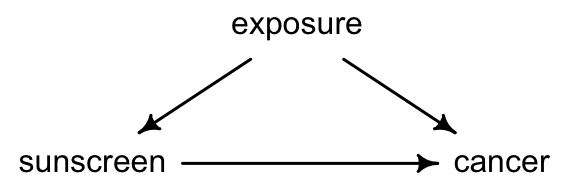
\includegraphics{Research-Design---Statistics_files/figure-latex/c4c11-1} 

}

\caption{DAG for effects of sunscreen use and sun exposure on skin cancer risk.}\label{fig:c4c11}
\end{figure}

If exposure increases the use of sunscreen and increases the risk of skin cancer, then that can generate an unexpected pattern of skin cancer being more common with sunscreen use! But let's say that sunscreen does have a direct causal effect of reducing skin cancer risk. If both forces are at play - the direct effect of sunscreen reducing cancer risk, and the confounding effect of sun exposure increasing sunscreen use and cancer risk - then you might not find any relationship at all between cancer risk and sunscreen use. In other words, sometimes confounders will \textbf{mask} a true causal effect, specifically if the pattern of the association between X and Y generated by the confounder is the opposite direction of the pattern of the association between X and Y generated by the direct effect.

\textbf{\emph{Identifying confounders on back-door paths:}} Confounders can be identified by finding \textbf{back-door paths} from the explanatory variable to the response variable. A back-door path is any path in the DAG that starts with an arrow pointing into the explanatory variable and ends with an arrow pointing into the response variable. Forks create backdoor paths: \(sunscreen \gets exposure \to cancer\).

Back-door paths can include more than two pathways. Consider a researcher trying to understand the causal effect of exercise on recovery time from a respiratory virus. Of course there are multiple potential common causes of exercise and viral recovery time. Figure \ref{fig:c4c12} shows a DAG that includes the expected causal effect of exercise on recovery time, but also general health knowledge and vaccination status. See if you can find the back-door path between exercise and recovery.

\begin{figure}

{\centering 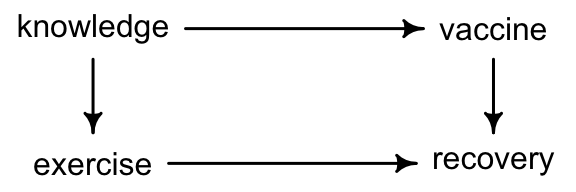
\includegraphics{Research-Design---Statistics_files/figure-latex/c4c12-1} 

}

\caption{DAG for causal effect of exercise on recovery time from a respiratory virus.}\label{fig:c4c12}
\end{figure}

The back-door path is \(exercise \gets knowledge \to vaccine \to recovery\). The confounder here is health knowledge. People with a lot of health knowledge might exercise more and be more likely to get vaccinated, and vaccination time can reduce recovery time. If that's the case, health knowledge confounds the relationship between exercise and recovery time. In this case, the back-door path includes more than one intervening node between the explanatory and response variable.

\textbf{\emph{Dealing with confounders:}} When there's a back-door path identified in a DAG that will confound the relationship between the explanatory and response variable, that pathway must be blocked or controlled. The options for blocking back-door paths involving confounders include study design and statistical analysis and will be addressed in coming chapters.

\subsection{The pipe: mediators}\label{the-pipe-mediators}

Let's continue examining the last DAG on viral recovery time to illustrate the next causal structure: the \textbf{pipe}. The pipe has a standard structure of \(X \to Z \to Y\). The variable Z is called a \textbf{mediator}, because the causal effect of X on Y is mediated (at least in part) by Z. You've probably noticed this structure in some of the DAGs we've explored so far. For example, the path \(knowledge \to exercise \to recovery\) is a pipe. Here, the causal effect of health knowledge is mediated by exercise. Essentially, the causal effect of knowledge is transmitted to viral recovery via exercise level. The path \(knowledge \to vaccine \to recovery\) is also a pipe. In this case, vaccination is a mediator transmitting the causal effect of knowledge to recovery.

When the causal effect of a variable X on Y involves a mediator Z, we call the causal effect of X on Y an \textbf{indirect effect}. A causal effect of X on Y can involve multiple indirect effects. Thus, one can examine the indirect effect of knowledge on recovery via exercise, or the indirect effect of knowledge on recovery via vaccination. Note that there is no direct effect of knowledge on recovery in this model.

Causal effects of a variable X on Y can also involve direct and indirect effects. Consider an ecologist asking whether the amount of forest habitat in a landscape causally affects bird species diversity. The researcher hypotheses that forest can affect species diversity in two ways. First, forest area can directly affect species diversity because the amount of forest affects the amount of resources available for birds (e.g., food, nesting sites). Second, forest area can indirectly affect species diversity by affecting the degree of habitat fragmentation. When forest area declines, the remaining forest becomes spatially fragmented, and fragmentation can have a direct effect on diversity by limiting the immigration of new species. Figure \ref{fig:c4c13} shows a DAG reflecting these ideas.

\begin{figure}

{\centering 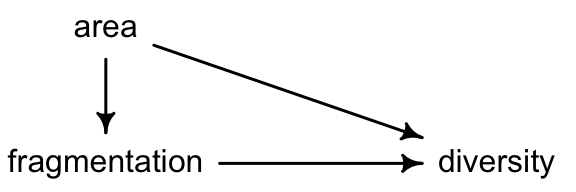
\includegraphics{Research-Design---Statistics_files/figure-latex/c4c13-1} 

}

\caption{DAG for causal effect of forest area and fragmentation on bird diversity.}\label{fig:c4c13}
\end{figure}

In this case, forest area has a direct effect on diversity and an indirect effect on diversity via the mediator fragmentation. The sum of a variables direct and indirect effects is called the \textbf{total effect}.

\textbf{\emph{Dealing with mediators:}} When the causal effect of X on Y involves a pipe, generally there is no need to do anything about the mediator. A mediator is an important component of the causal effect of the explanatory variable of interest. If I want to know the total effect of forest area on bird species diversity, then I should make sure that area can affect bird diversity in all the ways I hypothesize, including the direct effect and the indirect effect via fragmentation. If I block the effect of fragmentation on diversity as part of the research design or analysis, then I am blocking part of the causal effect of forest area on diversity. This is called \textbf{post-treatment bias}. The ``bias'' part of this phrase means that you would get the wrong answer if you wanted to know the total effect of area on diversity but blocked the effect of fragmentation. If you want to know either the total (or indirect effect) of a treatment variable (another term for an explanatory variable), then you need to let the causal effect of that treatment variable be transmitted through its mediators.

In some circumstances it is OK to block a mediators effect. For example, suppose I was specifically interested in the direct effect of forest area on bird diversity, independent of its effect via fragmentation. In that case, I would want to design the study or analysis in a way to block the pipe involving fragmentation, leaving only the direct effect of area on diversity.

\subsection{The inverted fork: colliders}\label{the-inverted-fork-colliders}

Imagine a researcher asks whether people who have serious illnesses (e.g., heart disease, cancer, autoimmune disorders) are more likely to be infected with COVID-19 than people who don't have serious illnesses. The researcher conducts the study by examining patient records from a local hospital and finds a surprising result: there's a \textbf{negative association} between serious illnesses and COVID-19. In other words, people who have serious illnesses appear \textbf{less} likely to have COVID-19 than those without a serious illnesses. But there's one problem with this analysis: it's not correct! Let's explore why with a simulated dataset.

Assume that serious illness status and COVID-19 status are binary categorical variables, and additionally assume that having a serious illness \textbf{increases} the probability of having COVID-19. Let's also assume that having a serious illness or COVID-19 increases the probability of someone being admitted to the hospital. Figure \ref{fig:c4c14} shows a DAG reflecting these assumptions.

\begin{figure}

{\centering 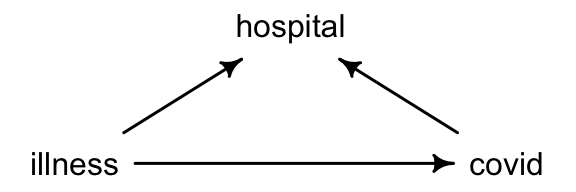
\includegraphics{Research-Design---Statistics_files/figure-latex/c4c14-1} 

}

\caption{DAG for the causal effect of serious illness on COVID infection status.}\label{fig:c4c14}
\end{figure}

And now here's the R code to generate some data based on the stated assumptions, using the \texttt{rbinom} function to simulate binary data just like in the example on greenspace and mental health outcomes.

\begin{Shaded}
\begin{Highlighting}[]
\FunctionTok{set.seed}\NormalTok{(}\DecValTok{123}\NormalTok{)}

\DocumentationTok{\#\# simulate illness status}
\NormalTok{ill }\OtherTok{\textless{}{-}} \FunctionTok{rbinom}\NormalTok{(}\AttributeTok{n =} \DecValTok{1000}\NormalTok{, }\AttributeTok{size =} \DecValTok{1}\NormalTok{, }\AttributeTok{prob =} \FloatTok{0.2}\NormalTok{)}

\DocumentationTok{\#\# simulate covid status based on illness status}
\NormalTok{cov }\OtherTok{\textless{}{-}} \FunctionTok{rbinom}\NormalTok{(}\AttributeTok{n =} \DecValTok{1000}\NormalTok{, }\AttributeTok{size =} \DecValTok{1}\NormalTok{, }\AttributeTok{prob =} \FunctionTok{ifelse}\NormalTok{(ill }\SpecialCharTok{==} \DecValTok{1}\NormalTok{, }\FloatTok{0.2}\NormalTok{, }\FloatTok{0.1}\NormalTok{))}

\DocumentationTok{\#\# simulate hospital status based on illness status and covid status}
\NormalTok{hos }\OtherTok{\textless{}{-}} \FunctionTok{rbinom}\NormalTok{(}\AttributeTok{n =} \DecValTok{1000}\NormalTok{, }\AttributeTok{size =} \DecValTok{1}\NormalTok{, }\AttributeTok{prob =} \FunctionTok{ifelse}\NormalTok{(ill }\SpecialCharTok{==} \DecValTok{1} \SpecialCharTok{\&}\NormalTok{ cov }\SpecialCharTok{==} \DecValTok{1}\NormalTok{, }\FloatTok{0.29}\NormalTok{, }
                                         \FunctionTok{ifelse}\NormalTok{(ill }\SpecialCharTok{==} \DecValTok{1} \SpecialCharTok{\&}\NormalTok{ cov }\SpecialCharTok{==} \DecValTok{0}\NormalTok{, }\FloatTok{0.25}\NormalTok{,}
                                         \FunctionTok{ifelse}\NormalTok{(ill }\SpecialCharTok{==} \DecValTok{0} \SpecialCharTok{\&}\NormalTok{ cov }\SpecialCharTok{==} \DecValTok{1}\NormalTok{, }\FloatTok{0.05}\NormalTok{, }\FloatTok{0.01}\NormalTok{))))}
\end{Highlighting}
\end{Shaded}

Here are the quantitative assumptions we've made in this simulated dataset of 1000 people:

\begin{enumerate}
\def\labelenumi{\arabic{enumi}.}
\tightlist
\item
  The baseline probability of someone having a serious illness is 20\%.
\item
  Serious illness increases the risk of COVID infection. The probability of a COVID infection is 20\% for those with a serious illness and 10\% for everyone else.
\item
  Serious illness and COVID both increase the chance of being admitted to the hospital. The baseline probability of someone without a serious illness or COVID being admitted to the hospital is assumed to be 1\%. A serious illness increases the risk by 24\%, and a COVID infection increases the risk by 4\%. Thus, if someone has COVID but no serious illness (\texttt{ill\ ==\ 0\ \&\ cov\ ==\ 1}), their chance of being in the hospital is 5\%. If someone has a serious illness but not COVID (\texttt{ill\ ==\ 1\ \&\ cov\ ==\ 0}), their chance of being in the hospital is 25\%. If someone has a serious illness and COVID (\texttt{ill\ ==\ 1\ \&\ cov\ ==\ 1}), their chance of being in the hospital is 29\%.
\end{enumerate}

Now let's replicate the researcher's analysis by filtering the dataset to only include hospitalized patients, and then we will examine the relationship between serious illness and COVID status:

\begin{Shaded}
\begin{Highlighting}[]
\NormalTok{d }\OtherTok{\textless{}{-}} \FunctionTok{cbind.data.frame}\NormalTok{(ill, cov, hos) }\CommentTok{\#create a data frame with all 3 variables}
\NormalTok{hos.patients }\OtherTok{\textless{}{-}}\NormalTok{ d[d}\SpecialCharTok{$}\NormalTok{hos }\SpecialCharTok{==} \DecValTok{1}\NormalTok{,] }\CommentTok{\#extract the observations for the hospital patients}

\FunctionTok{addmargins}\NormalTok{(}\FunctionTok{table}\NormalTok{(hos.patients}\SpecialCharTok{$}\NormalTok{ill, hos.patients}\SpecialCharTok{$}\NormalTok{cov,}
                 \AttributeTok{dnn =} \FunctionTok{c}\NormalTok{(}\StringTok{"ill"}\NormalTok{, }\StringTok{"cov"}\NormalTok{)))}
\end{Highlighting}
\end{Shaded}

\begin{verbatim}
##      cov
## ill    0  1 Sum
##   0    8  4  12
##   1   47 12  59
##   Sum 55 16  71
\end{verbatim}

From the filtered dataset, we can see that we have a total of 71 hospital records. Of the 71 patients, 47 patients have a serious illness but not COVID, 4 patients have COVID but not a serious illness, and 12 patients have a serious illness and COVID. Does having a serious illness increase the risk of COVID?

If we simply compute the probability of COVID for people with and without a serious illness, here's what we find. The probability of COVID is 12/59 = 20\% for people with a serious illness and 4/12 = 33\% for people without a serious illness. That's right. Among hospitalized patients, people without a serious illness appear more likely to have COVID than those with a serious illness, the opposite of the true relationship in the general population based on our simulated model.

This counterintuitive result arises from \textbf{collider bias}. Take another look at the DAG and note that both serious illness and COVID status causally affect hospital admission: \(Illness \to Hospital \gets COVID\). This causal structure is called an inverted fork: \(X \to Z \gets Y\), where the variable Z is called a \textbf{collider} because it is causally affected by both X and Y. Hospital admission is a collider, where a patient is most likely to be admitted if they have a serious illness or COVID.

\textbf{\emph{Dealing with colliders:}} Colliders only create problems when a researcher blocks or controls for the collider Z in the pathway \(X \to Z \gets Y\) as part of the research design or analysis. That's exactly what's happening with our example case of filtering the dataset to only individuals who were admitted to the hospital. When conditioning on hospital admissions in this way, a spurious relationship is generated between serious illness and COVID status.

Think about it this way. When we restrict the analysis to hospitalized patients, the two causes of hospitalization compete in a away to explain why patients were admitted. If a patient doesn't have COVID, they must have had a serious illness. If a patient doesn't have a seriuos illness, they must have had COVID. This creates a spurious negative relationship between serious illness and COVID status, even though the true relationship in the general population is just the opposite.

Collider bias is a type of \textbf{selection bias} in that it's driven by analyzing relationships between variables within a certain group. The world is full of these kind of examples. Why do ex-partners tend to either be attractive or intelligent, but not both? In this case the sample is restricted only to the people you dated in the past. If an ex wasn't particularly attractive, they were probably intelligent. If an ex wasn't intelligent, they were probably attarctive. Individuals who were neither attractive nor intelligent never made it into the pool of individuals you'd choose to go on a date with!

So beware of colliders. When you are interested in the causal relationship between X and Y, and X and Y both affect Z, generally avoid filtering the dataset by Z!

\section{Closing backdoor paths}\label{closing-backdoor-paths}

Drawing a DAG is a really useful way of being explicit about your scientific model, but it can also inform how you should go about designing your study and analyzing data. That's ultimately why we're covering graphical causal diagrams before we jump into statistics. DAGs represent your causal assumptions, and everything else - design, analysis, inference - follows from that. Science before statistics!

Once you have a DAG in hand, you can evaluate it to identify problematic pathways, basically any causal path that confounds the causal effect of interest. The causal pathways of interest start with a particular explanatory variable X and end with an outcome variable Y, and the arrows between X and Y should be forward facing. We will call these pathways \textbf{directed paths}, which are causal and of primary interest. This might involve a direct effect of X on Y, \(X \to Y\), indirect effects of X on Y \(X \to Z \to Y\), or both (the total effect). Problematic pathways are \textbf{back-door paths}, which are paths that connect X to Y but start with an arrow pointing into X. A fork structure with a confounder is the classic example. Back-door paths are noncausal and must be blocked. Finally, some paths between X and Y will start with a directed path out of X but end with a collider. If there's a collider on a pathway between X and Y, that pathway is noncausal but is already blocked. No further action is needed.

Let's take a look at an example. Figure \ref{fig:c4c17} shows a DAG where the interest is in understanding the causal effect of screen time on obesity in pediatric patients (\href{https://www.nature.com/articles/s41390-018-0071-3}{Williams et al.~2018}). The DAG includes three other relevant variables, parent education, physical activity, and self-harm. This DAG represents a scientific hypothesis about the causal relationship between screen time and obesity, but it also includes other relevant pathways that are noncausal but could generate a spurious association between screen time and obesity. To understand how best to proceed with the design and analysis phase of the research, one would start by listing all the pathways between screen time and obesity, then identify the causal pathways of interest and the noncausal pathways. Given a list of all the pathways, causal and noncausal, one can then determine if any action needs to be taken to block the noncausal pathways from generating spurious associations.

\begin{figure}

{\centering 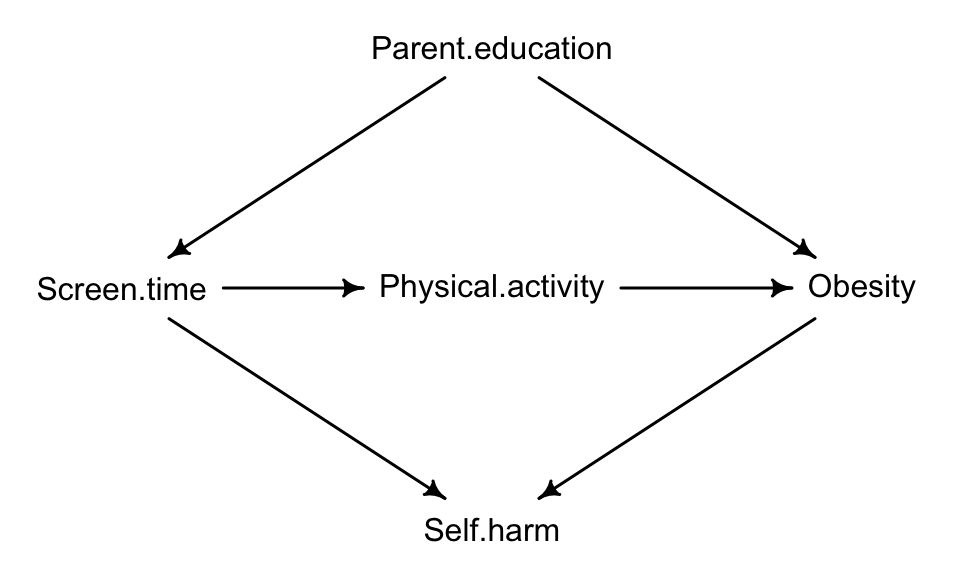
\includegraphics{Research-Design---Statistics_files/figure-latex/c4c17-1} 

}

\caption{DAG for the causal effect of screen time on obesity in pediatric patients.}\label{fig:c4c17}
\end{figure}

Below I list every path connecting the explanatory variable (screen time) to the response variable (obesity). For each path, we identify whether it is directed, back-door, or blocked via a collider. Given this information, one can decide which variables should be controlled during the design or analysis phase, and which variables should be left alone.

\begin{itemize}
\item
  \(Screen.time \to Physical.activity \to Obesity\): Here we have a pipe. This is a forward causal pathway involving an indirect effect of screen time on obesity via physical activity. The hypothesis here is that the more time a child spends on a screen, the less time they are being physically active, and the more likely they will be obese. This is a causal pathway of interest, so we wouldn't want to block it. It would be a mistake to block or condition on physical activity, because that's assumed to be an essential component of the causal mechanism linking screen to obesity. Blocking physical activity would be an example of post-treatment bias.
\item
  \(Screen.time \gets Parent.education \to Obesity\): This is a back-door path because it involves an arrow pointing into the explanatory variable. The causal structure is a fork, where parent education is a confounder. Thus, this is a non-causal path that will generate a spurious association between screen time and obesity. We need to block the effect of parent education on obesity during the design or analysis phase of the research.
\item
  \(Screen.time \to Self.harm \gets Obesity\): This is a path involving a collider. Note that both screen time and obesity are assumed to have direct effects on self-harm. Collider paths are blocked by default, so no action is necessary. It would be a mistake to design the research or conduct the analysis in a way that conditions on self-harm (for example, by only analyzing individuals who have a history of self-harm), because that would generate a noncausal association between screen time and obesity.
\end{itemize}

There you have it. With a DAG in hand, you can identify all the potential paths bewteen the explanatory and response variable, and determine for each whether not they need to be blocked. We will examine the methods of blocking available when we explore study designs and linear models later in the book.

\section{Like all models, DAGs require assumptions}\label{like-all-models-dags-require-assumptions}

The great value of using DAGs is that they make causal assumptions crystal clear. Based on those assumptions and the causal structures observed in a DAG, one can design a data colleciton scheme or analyze the data in a way that increases the chance of obtaining an unbiased estimate of the causal effect of interest. But like all models, DAGs are simplifications of nature and have their own assumptions. Here are some important ones:

\begin{enumerate}
\def\labelenumi{\arabic{enumi}.}
\item
  Causal effects in DAGs cannot be bidirectional. They must be \textbf{directed} from one variable to another.
\item
  DAGs cannot have cycles. In other words, you can't have a causal effect structure like this where you start with a causal effect of variable X and have a chain of causal effects that end back at X: \(X \to Y \to Z \to X\). Cycles or loops are not allowed. DAGs are most beneficial to represent static causal models. If your scientific hypothesis is more dynamic, involving time and feedback loops, other tools for causal inference will often be necessary.
\item
  All variables with non-trivial effects should be included. This is most important when two variables have a shared cause, like Z here: \(X \gets Z \to Y\). The reason it's important to include common causes is because such confoudners need to be blocked by design or in the analysis to get an unbiased estimate of the relationship between X and Y. Unobserved or unmeasured confounders will lead to biased conclusions, although there are methods to help address unobserved confounders.
\item
  Building on the previous point, using a DAG to inform research design and analysis does not magically make any association you find a causal relationship. Leaving non-trivial variables out of the DAG, particularly confounders, will make causal conclusions from the DAG invalid. Domain knowledge becomes extremely important when designing a DAG to ensure that it adequately represents prior knowledge about the science of the research question.
\end{enumerate}

So DAGs have assumptions and limits like any model, but they are a very useful method for an initial exploration of the tools of causal inference. We'll build on this foundation moving forward.

\chapter{Elements of Research Design: Study Type}\label{elements-of-research-design-study-type}

So far we have examined the importance of identifying a clear research question and communicating the causal assumptions related to the research question with a DAG. I've tried to make the case that defining clear research questions and developing an explicit scientific model as a DAG will help inform how one goes about designing research to collect and analyze data. In the next two chapters, we will begin to look at some basic elements of research design given a question and DAG in hand. We'll first explore our options for different types studies we can conduct, and then we'll explore the concept of sampling to collect data and some principles we can apply to maximize the quality of our dataset and the inferences we make from the data. Let's begin with study design.

\section{Types of Study Designs}\label{types-of-study-designs}

Consider the last research question from Chapter 4 on graphical causal models: Does screen time affect obesity in children? The hypothesis here is that screen time increases obesity due to reduced physical activity. Time is a zero sum game. Children who spend four hours on a screen each day are not spending those four hours being physically active, and increased risk of obesity may be a consequence of reduced physical activity. In the terms of a DAG in Figure \ref{fig:c5c1}, the expectation is that screen time indirectly increases obesity by reducing physical activity, where physical activity is a mediator.

\begin{figure}

{\centering 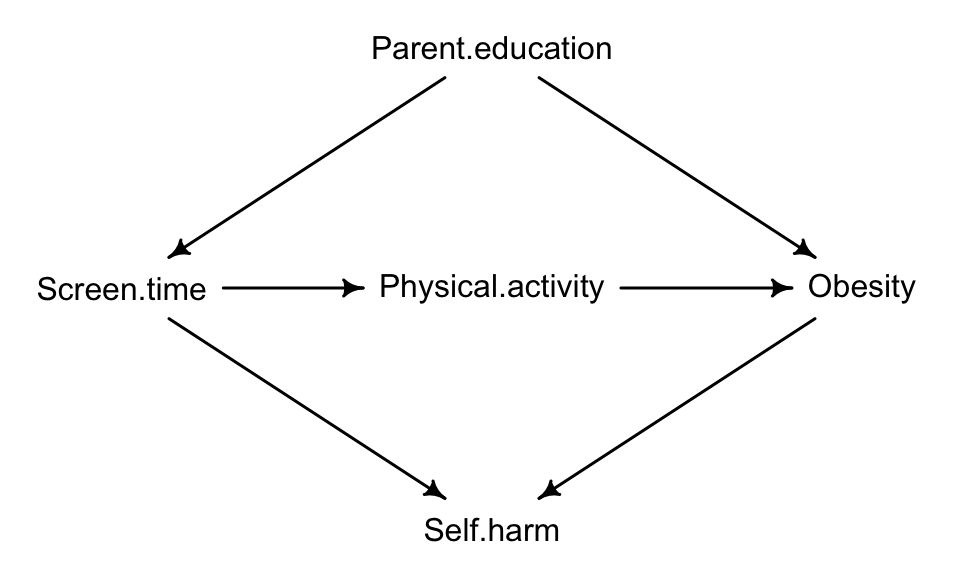
\includegraphics{Research-Design---Statistics_files/figure-latex/c5c1-1} 

}

\caption{DAG for the causal effect of screen time on obesity in pediatric patients.}\label{fig:c5c1}
\end{figure}

The DAG from Chapter 4 also includes two additional variables that are causally related the explanatory and response variable. Screen time and obesity are both expected to have direct effects on self-harm. Because self-harm is a collider in this DAG, and the path \(Screen.time \to Self.harm \gets Obesity\) is blocked by default. In other words, when we design the research, we should \textbf{not} attempt to do anything additionally in our research design to block the self-harm outcome. Doing so would actually create a noncausal association between screen time and obesity.

The other relevant path in the DAG is \(Screen.time \gets Parent.education \to Obesity\). This is a back-door path with a confounding effect of parent education. Here the idea is that parents with a lot of education about health will know something about the risks of screen time and the risks of obesity, and they may take actions to minimize screen time and obesity in their children through mechanisms other than physical activity. For example, perhaps the parents who restrict screen time are also likely to restrict their children's diet to the most health foods. If that were the case, you might find a positive association between obesity and screen time. But that positive association wouldn't reflect the causal effect of screen time.

Given this DAG and the potential confounding effect of parental education, how do we proceed to design the study? There are two general types of study designs we can use: experimental and observational research.

\section{Experimental studies}\label{experimental-studies}

\textbf{\emph{Experiments}} are essentially the gold standard for scientific research when the goal is causal explanation. There are two key elements of experiments. First, the researcher manipulates the explanatory variable. In other words, individuals in the experiment are assigned particular values of the explanatory variable, often referred to as the \textbf{treatment}. Second, the particular values of the explanatory varaible are \textbf{randomly assigned} to individuals in the experiment. This element is called \textbf{randomization}, and it is really the defining feature of an experiment.

Why is randomization so important? Let's consider this question in the context of the research question on screen time and obesity. The DAG shows that parent education is a confounding variable. Thus, the concern is that kids who have low levels of screen time have parents with high levels of education, and those parents with high education parent in other ways (besides screen time) to minimize the chance that their kids will be obese. If the researcher is interested in the effect of screen time on obesity, then the confounding effect of parent education must be controlled. And that's what randomization does.

Suppose the researcher enrolls 200 kids into the study. The researcher decides that she will assign three possible levels of screen time: 0, 5, or 10 hours per week. These different levels of screen time will be assigned to each participant randomly. For example, the researcher might have a list of each individual's name (or more likely, an identification code), and for each individual she could pick a piece of paper out of a hat indicating one of the three treatment levels. Or, she can use 21st-century technology and assign one of the three treatment levels in R:

\begin{Shaded}
\begin{Highlighting}[]
\FunctionTok{set.seed}\NormalTok{(}\DecValTok{123}\NormalTok{)}
\DocumentationTok{\#\# create ID codes for each participant}
\NormalTok{id }\OtherTok{\textless{}{-}} \DecValTok{1}\SpecialCharTok{:}\DecValTok{200}

\DocumentationTok{\#\# define the three treatment levels (0 = none, 5 = low, 10 = high)}
\NormalTok{trt.levels }\OtherTok{\textless{}{-}} \FunctionTok{c}\NormalTok{(}\StringTok{"none"}\NormalTok{, }\StringTok{"low"}\NormalTok{, }\StringTok{"high"}\NormalTok{)}

\DocumentationTok{\#\# randomly assign each individual to a treatment}
\NormalTok{trt }\OtherTok{\textless{}{-}} \FunctionTok{sample}\NormalTok{(trt.levels, }\DecValTok{200}\NormalTok{, }\AttributeTok{replace =} \ConstantTok{TRUE}\NormalTok{)}

\DocumentationTok{\#\# combine into a dataframe}
\NormalTok{d }\OtherTok{\textless{}{-}} \FunctionTok{cbind.data.frame}\NormalTok{(id, trt)}
\FunctionTok{head}\NormalTok{(d)}
\end{Highlighting}
\end{Shaded}

\begin{verbatim}
##   id  trt
## 1  1 high
## 2  2 high
## 3  3 high
## 4  4  low
## 5  5 high
## 6  6  low
\end{verbatim}

The \texttt{sample} function was used to randomly assign each of the 200 participants to one of the three treatment levels \footnote{The \texttt{replace} = TRUE argument just means that the sampling is done ``with replacement''. That means if the first person is assigned the ``high'' treatment, the next person can also be assigned the ``high'' treatment.}. Here's why randomization is the key feature of an experiment: If the treatment levels are randomly assigned to each individual, then there will be no relationship between the screen time of each participant and their parent's education level. A participant with who has highly educated parents will have an equal chance of being assigned to each of the three levels of screen time. In other words, experiments remove the influence of confounding variables on the explanatory variable. If the researcher used an experiment in this way, the DAG would be revised to eliminate the \(Parent.education \to Screen.time\) effect as seen in Figure \ref{fig:c5c3}.

\begin{figure}

{\centering 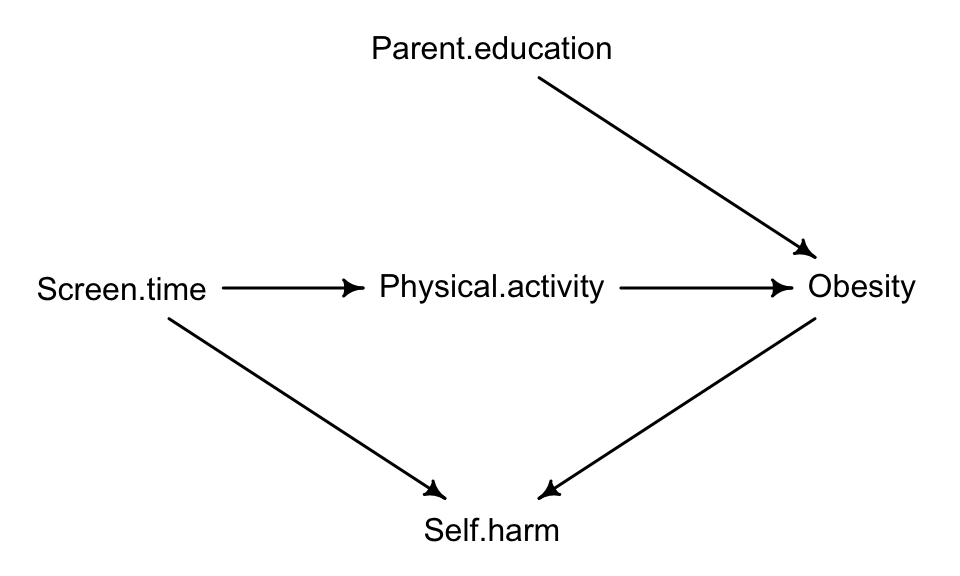
\includegraphics{Research-Design---Statistics_files/figure-latex/c5c3-1} 

}

\caption{DAG for the causal effect of screen time on obesity in pediatric patients when using an experimental study design.}\label{fig:c5c3}
\end{figure}

In this revised DAG, there is no longer a back-door path confounding the relationship between screen time and obesity. The research would randomly assign the levels of screen time, let enough time pass to observe the expected effect, and then record the value of the outcome variable, obesity (likely as the change in obesity from the start to the end of the study).

Random assignment of the explanatory varaible to individuals in an experiment not only helps control for confounding variables the researcher is aware of, but also unobserved confounders. Even with extensive domain knowledge, it's hard to think about every possible confounding variable and to include each one in the DAG. Randomization breaks the association between the explanatory varaible and unobserved confounders too.

Experiments are sometimes referred to as \textbf{randomized controlled trials (RCTs)}, emphasizing the essential component of randomization when attempting to infer a causal effect of an explanatory variable. The ``controlled'' part of the RCT name often refers to a \textbf{control group}, which is a group that does not receive the standard treatment. Control groups are often essential as a baseline for comparison. In the experiment described here on screen time and obesity, the ``none'' category of screen time is the control group. However, experiments don't always need a control group as traditionally defined. For example, suppose that instead of ``none'', ``low'', and ``high'', we just dropped the ``none'' category and assigned individuals to one of two treatment levels: low and high screen time. The researcher would still randomly assign these two levels of screen time to participants and then compare the change in obesity between the two groups. The ``low'' treatment functions as the baseline for comparison. A researcher might not include a traditional control group (complete absence of the treatment) if that's not a realistic value in the target population of interest, such as if the study is being conducted on a population where virtually no children have exactly zero screen time.

Although experiments are the goal standard of causal inference, correct causal inference isn't a guarantee. One problem researchers face is when participants in an experiment don't comply with their treatment instructions. This kind of issue can be common in experiments requiring behavioral compliance of people (e.g., psychology; \href{https://compass.onlinelibrary.wiley.com/doi/epdf/10.1111/spc3.12948}{Rohrer 2023}). For example, imagine that some individuals who were assigned to the ``none'' treatment still give their kids some screen time. When compliance is a potential issue, researchers should collect data on both the treatment level randomly assigned \emph{and} the treatment level actually received. Hopefully participatns are honest, and the person assigned to the ``none'' treatment level reports their actual screen time.

But even if people are honest and report their actual screen time, the noncompliance introduces significant complication for the analysis. Although the treatment levels were randomly assigned to participants, the noncompliance may not be random. What if noncompliance is affected by parental education? In this case, perhaps the most highly educated parents enforce stricter screen time limitations than the treatment they were assigned, where as parents with less education may be more likely to relax a strict limitation and allow their kids to have more screen time. The DAG in Figure \ref{fig:c5c4} below is modified to reflect this possibility, now including a variable for the actual screen time experienced by the participants, and a direct causal effect of parent education on actual screen time. The researcher might have been aware of noncompliance and collected data on \emph{actual} screen time, but it would be a mistake to simply analyze the relationship between obesity and actual screen time. Why? There's a backdoor path from actual screen time to obesity via the confounder, parent education. Even in an experimental context, correctly analyzing the causal effect of screen time in this example would require an analysis that controls for the effect of parental education on actual screen time.

\begin{figure}

{\centering 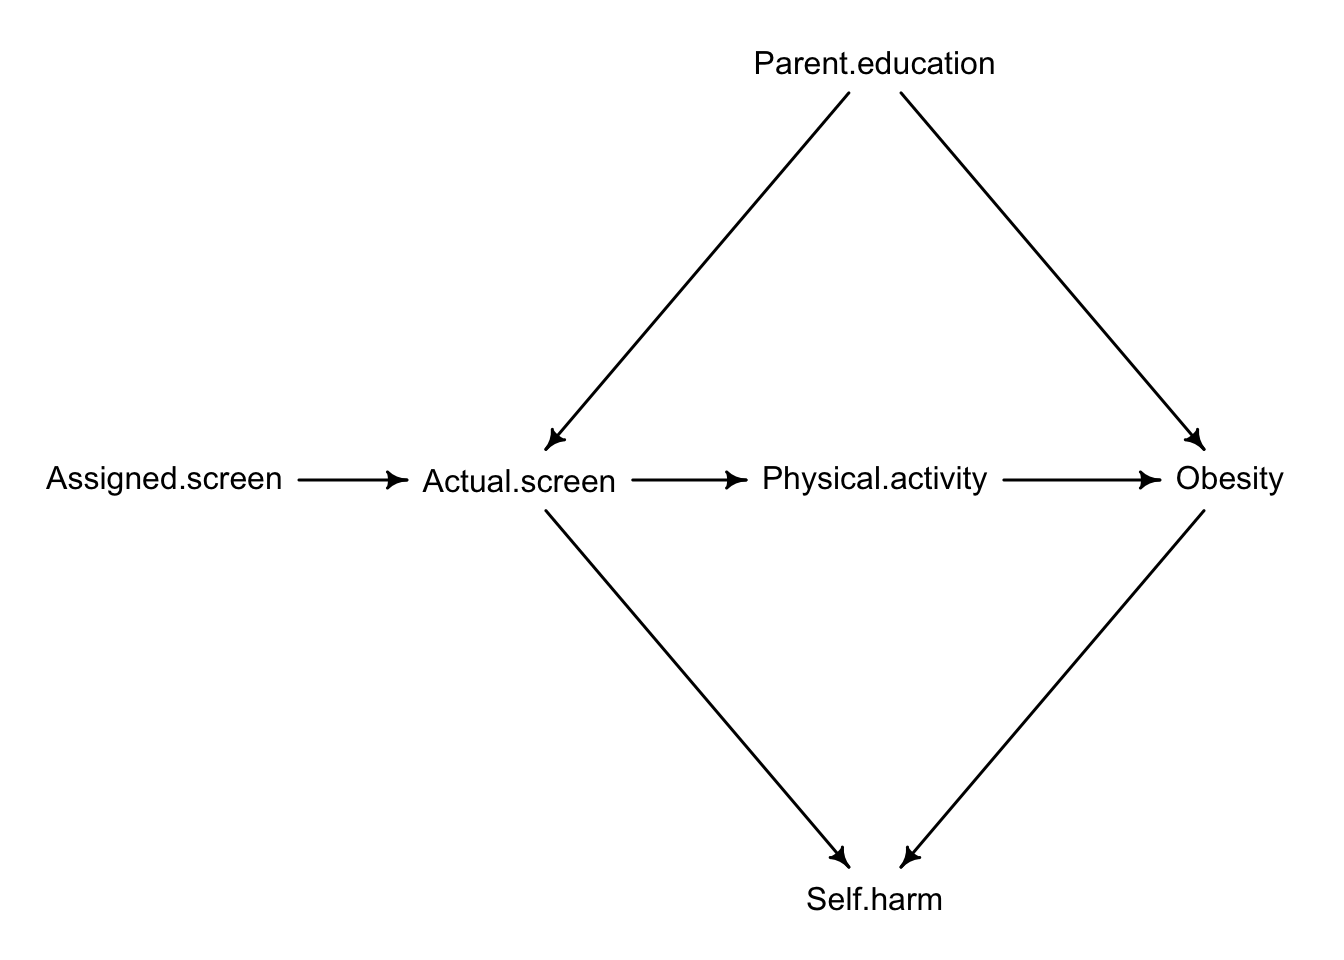
\includegraphics{Research-Design---Statistics_files/figure-latex/c5c4-1} 

}

\caption{Revised DAG including actual screen time.}\label{fig:c5c4}
\end{figure}

So, experiments aren't a guarantee of safe causal inference, even when treatments are randomly assigned. Moreover, sometimes conducting experiments can be challenging, or even impossible. Imagine you're an economist studying the effect of the minimum wage on employment. It's impossible to randomly assign different minimum wages to different municipalities. If you're a biologist studying the effect of urbanization on biodiversity, you can't randomly assign areas that do and do not become urbanized. Sometimes experiments can't be done because they're unethical. If you're a psychologist studying the effect of parenting style and child personality, you can't randomly assign babies to different parenting styles. In cases like these, researchers have to rely on observational designs, which we turn to next.

\section{Observational studies}\label{observational-studies}

When researchers collect data without randomly assigning levels of the explanatory variable to individuals, they are conducting an \textbf{\emph{observational study}}. The key element making a study observational is when the researcher has no role in determining how the data arose. The data arose naturally and are observed and recorded by the reseacher. Sometimes you have to take what you can get.

How would an observational design be conducted to address our research question on screen time and obesity. There's a couple ways such a study could proceed. One approach would be to enroll individuals into a study and track their screen time and obesity over time. This kind of design is called a \textbf{prospective study}, which is simply a study that is planned in advance. Another approach would be to analyze existing data on screen time and obesity. Perhaps a dataset was previously collected by these factors by another researcher, or by a medical doctor in their own practice. This kind of design is called a \textbf{retrospective study}, referring to the fact that the data being analyzed were generated in the past. Both of these designs have the common element of the data arising naturally on their own without the researcher randomly assigning levels of screen time.

In some ways observational studies are much easier to pull off, particularly if a dataset is already available. But observational designs can present significant challenges in interpretation. Because the levels of the explanatory variable are not randomly assigned, any back-door path involving a confounding variable is unblocked in an observational design. Sure, it might be easy to record screen time and obesity for a bunch of kids, but remember parental education? Kids that have knowledgeable parents might limit their screentime and enforce a diet that minimizes obesity. In that case, one would find a positive relationship between screen time and obesity, not because of a causal effect of screen time, but because of confounding effect of parental education. This is exactly what people mean when they say ``correlation is not necessarily causation''. In addition to generating noncausal correlations, it's also important to remember that confounders can also mask real relationships.

So how do we proceed to make causal inferences with an observational design? One needs to have a clear scientific model of their system that makes causal assumptions clear, such as with a DAG. With a well-defined DAG that identifies likely back-door paths and confounders, one can then block those paths during the analysis phase. We won't learn the methods to do that until later in the book, but at this point it's important to understand that the researcher must identify potential confounders \emph{and} measure them in order to apply the methods we'll use to block back-door paths during analysis. That's why researchers should start by defining a DAG before the data are collected.

\subsection{Pros and cons of prospective vs.~retrospective studies (planned)}\label{pros-and-cons-of-prospective-vs.-retrospective-studies-planned}

\chapter{Elements of Research Design: Sampling Strategies}\label{elements-of-research-design-sampling-strategies}

At this point we know that effective research practice requires articulating a clear question, identifying causal assumptions about the relationship between response and explanatory variables, and proceeding with an experimental or observational study design. Once these issues are settled, it's time to think about data collection. But don't go so fast! The way in which one collects data goes a long way in determining the quality of data analysis and the uncertainty about our conclusions. In this chapter, we will take a close look at how data should be collected in a way that maximizes the quality of our data and minimizes the uncertainty in our conclusions.

\section{Inferences from data are (almost) always uncertain}\label{inferences-from-data-are-almost-always-uncertain}

I teach a statistics class as part of a biology curriculum, so the students in my class are either majoring in biology or something else. What proportion of the students in my class are biology majors? Hey - that's a research question! On it's own, it's not a very interesting research question, as it is purely descriptive. But for a variety of reasons, it is useful to know something about the background of students taking a course.

Notice that my question is very specific about \emph{who} I want to make conclusions about. What proportion of the students in \emph{my class} are biology majors? This is an example of a research question that is very limited in scope. In a typical semester, I have about 24 students in my statistics class. For my research question, those 24 students represent the \textbf{population} of interest. The target population is very specific and small.

Now suppose my research question is \emph{What proportion of all students taking a statistics class are biology majors?}. Now things are more complex. This research question is still descriptive - I simply want to know the value of a proportion - but now the scope is much broader. The statistical population for this question is now everyone who is taking a statistics class at the moment. Everyone where? Presumably everyone who is taking a statistics class at a university where a biology major is offered. Although notice that one could address this question for students taking a statistics class anywhere, whether or not there's a biology major offering. And what about the temporal scope of the question? Is it all students taking a statistics class \emph{right now}, over the last 5 years, or some other temporal scope? Remember that the population is basically the who, what, when, and where of your research question, and often it requires more detailed information beyond a simple one-sentence statement of the research question.

When the target population is very limited in scope, the design, analysis, and conclusions are often straightforward. Why? Well, it's not too hard to track down every student in my class of 24 and ask whether or not they are a biology major. In fact, I can just log onto my university's academic management system and obtain a record of the declared major of each student in the class. If 16 students are listed as biology majors and 8 students are not biology majors, then the proportion of biology majors in my class is simply 16/24 = 0.8 (80\%). I can answer my research question with virtual certainty, mainly because my target population is so limited in scope. Now I wouldn't say that I'm \emph{completely} certain that exactly 80\% of the students in my class are biology majors. Why not? There are a number of reasons. It's possible that the records are not all correct. It's possible that someone is classified as a biology major by mistake. Or maybe a student dropped the class, but that wasn't updated in the records at the time I retrieved the data. In other words, even when the target population is limited, there's almost always some sources of uncertainty.

Usually there's more uncertainty as the target population of inference grows larger. Let's say I'm interested in the proportion of biology majors taking a statistics class this semester in North American universities. I've narrowed down the scope of the research question pretty well, and therefore I have a good sense of the who, what, when, and where I can generalize about based on my study. But now I'm faced with the challenge of collecting data in a way that adequately represents a very large population of interest. If I want to know the proportion of biology majors with the same degree of confidence that I had when I was focused only on my particular class, I'd have to track down every single statistics class in North American universities and then determine whether each student is a biology major or not. That's not going to happen. Logistically it is simply impossible to collect data from everyone in the population in this case.

This is basically the crux of the problem of why we need the field of statistics. We need statistics because most research questions involve populations that are too large to collect data from in their entirety. When the population is too big, we need to take a \textbf{sample} of individuals from the population to address the question. I can't track down every single statistics class, so instead I take a sample of statistics classes currently being offered and use that sample to \textbf{estimate} the proportion of biology majors. When I take a sample of statistics classes, inevitably there is going to be a difference between the proportion of biology majors that I estimate from the sample and the actual proportion of biology majors among all students taking statistics. And to the add to the problem, I'm still going to have to deal with some uncertainty about my measurements of the individuals that were included in my sample.

\section{Sampling requires estimation}\label{sampling-requires-estimation}

Consider a very simple case of coin flipping. With a fair coin, the probability of a coin landing on heads is 0.5. But let's just suppose you didn't know the probability of the coin landing on heads is 0.5. You're going to estimate the probability of the coin landing on heads through a process of sampling from 10 coin flips, recording the total number of heads out of the 10 flips. Is it possible to get 6 out of 10 heads, leading to 0.6 for the \textbf{estimated} probability of heads? Absolutely. Or you might get 3 out of 10 heads for an estimate of 3/10 = 0.3, or 5 out of 10 heads for an estimate of of 5/10 = 0.5. This is the problem of sampling - there will often be some variation between the estimate of the quantity of interest and the true value. That introduces uncertainty. If there's some error on my process of recording the outcome of each coin flip, then there will be even more uncertainty.

Let me show you exactly what I mean by simulating this exact situation. When we flip a coin, there are two possible outcomes, heads and tails. In other words, the variable in this case is categorical, and specifically it is binary because there are two possible outcomes. When we flip a coin 10 times, we can keep track of the number of heads (or tails - it doesn't matter), which will be anywhere from 0 to 10 heads. This process of counting the outcome of a binary variable across multiple trials is called a binomial function. Recall we can use the \texttt{rbinom} function to simulate sampling for a binary process:

\begin{Shaded}
\begin{Highlighting}[]
\DocumentationTok{\#\# flip a single coin (size = 1) 10 times (n = 10); the coin is fair (prob = 0.5)}
\FunctionTok{rbinom}\NormalTok{(}\AttributeTok{n =} \DecValTok{10}\NormalTok{, }\AttributeTok{size =} \DecValTok{1}\NormalTok{, }\AttributeTok{prob =} \FloatTok{0.5}\NormalTok{)}
\end{Highlighting}
\end{Shaded}

\begin{verbatim}
##  [1] 1 1 1 1 0 0 0 1 1 0
\end{verbatim}

In this case the function returns a vector of 1s and 0s. Let's define heads as 1 and tails as 0. In the simulation, the number of heads can be obtained by simply summing the number of 1s. Alternatively, we can define the arguments of the \texttt{rbinom} function to count the number of heads (1s) out of a single set of 10 flips:

\begin{Shaded}
\begin{Highlighting}[]
\DocumentationTok{\#\# flip a single coin (size = 1) 10 times (n = 10); the coin is fair (prob = 0.5)}
\FunctionTok{rbinom}\NormalTok{(}\AttributeTok{n =} \DecValTok{1}\NormalTok{, }\AttributeTok{size =} \DecValTok{10}\NormalTok{, }\AttributeTok{prob =} \FloatTok{0.5}\NormalTok{)}
\end{Highlighting}
\end{Shaded}

\begin{verbatim}
## [1] 3
\end{verbatim}

Cool. This isn't rocket science. Clearly you can flip a coin 10 times and count the number of heads without R, and intuitively you know that you won't always get exactly 5 heads out of 10 flips of a fair coin. But when we flip a coin 10 times, how often will we get 5 heads, or 4 heads, or 8 heads? You could flip a coin 10 times, count the number of heads, and repeat that process many times to get a sense of the relative frequency of the outcomes. But that will take you a long time! This is where we can harness the power of R. Let's simulate our coin flipping process of counting the number of heads out of 10 flips a total of 1 million times:

\begin{Shaded}
\begin{Highlighting}[]
\DocumentationTok{\#\# flip a single coin (size = 1) 10 times (n = 10); the coin is fair (prob = 0.5)}
\NormalTok{heads }\OtherTok{\textless{}{-}} \FunctionTok{rbinom}\NormalTok{(}\AttributeTok{n =} \DecValTok{1000000}\NormalTok{, }\AttributeTok{size =} \DecValTok{10}\NormalTok{, }\AttributeTok{prob =} \FloatTok{0.5}\NormalTok{)}
\NormalTok{heads[}\DecValTok{1}\SpecialCharTok{:}\DecValTok{20}\NormalTok{]}
\end{Highlighting}
\end{Shaded}

\begin{verbatim}
##  [1] 3 6 6 8 5 3 6 6 3 5 4 3 5 3 4 2 6 4 3 3
\end{verbatim}

Now we get a vector of 1 million observations, each recording the number of heads out of 10 flips. I'm showing you only the first 20 outcomes, but we can easily generate a table or graph to show the relative frequency of each outcome. Here are tables of the absolute count of each outcome, as well the probability of each outcome:

\begin{Shaded}
\begin{Highlighting}[]
\DocumentationTok{\#\# absolute count of outcomes}
\FunctionTok{table}\NormalTok{(heads)}
\end{Highlighting}
\end{Shaded}

\begin{verbatim}
## heads
##      0      1      2      3      4      5      6      7      8      9     10 
##    992   9712  44120 117823 204979 246133 204423 117305  43790   9723   1000
\end{verbatim}

\begin{Shaded}
\begin{Highlighting}[]
\DocumentationTok{\#\# probability (relative frequency) of outcomes}
\FunctionTok{prop.table}\NormalTok{(}\FunctionTok{table}\NormalTok{(heads))}
\end{Highlighting}
\end{Shaded}

\begin{verbatim}
## heads
##        0        1        2        3        4        5        6        7        8        9       10 
## 0.000992 0.009712 0.044120 0.117823 0.204979 0.246133 0.204423 0.117305 0.043790 0.009723 0.001000
\end{verbatim}

Figure \ref{fig:c6c5} shows a graphical view of the probability of each outcome.

\begin{Shaded}
\begin{Highlighting}[]
\FunctionTok{barplot}\NormalTok{(}\FunctionTok{prop.table}\NormalTok{(}\FunctionTok{table}\NormalTok{(heads)),}
        \AttributeTok{names.arg =} \FunctionTok{c}\NormalTok{(}\DecValTok{0}\SpecialCharTok{:}\DecValTok{10}\NormalTok{),}
        \AttributeTok{ylim=}\FunctionTok{c}\NormalTok{(}\DecValTok{0}\NormalTok{, }\FloatTok{0.25}\NormalTok{),}
        \AttributeTok{xlab =} \StringTok{"Number of Heads"}\NormalTok{, }\AttributeTok{ylab =} \StringTok{"Probability"}\NormalTok{,}
        \AttributeTok{col =} \StringTok{"skyblue"}\NormalTok{)}
\end{Highlighting}
\end{Shaded}

\begin{figure}
\centering
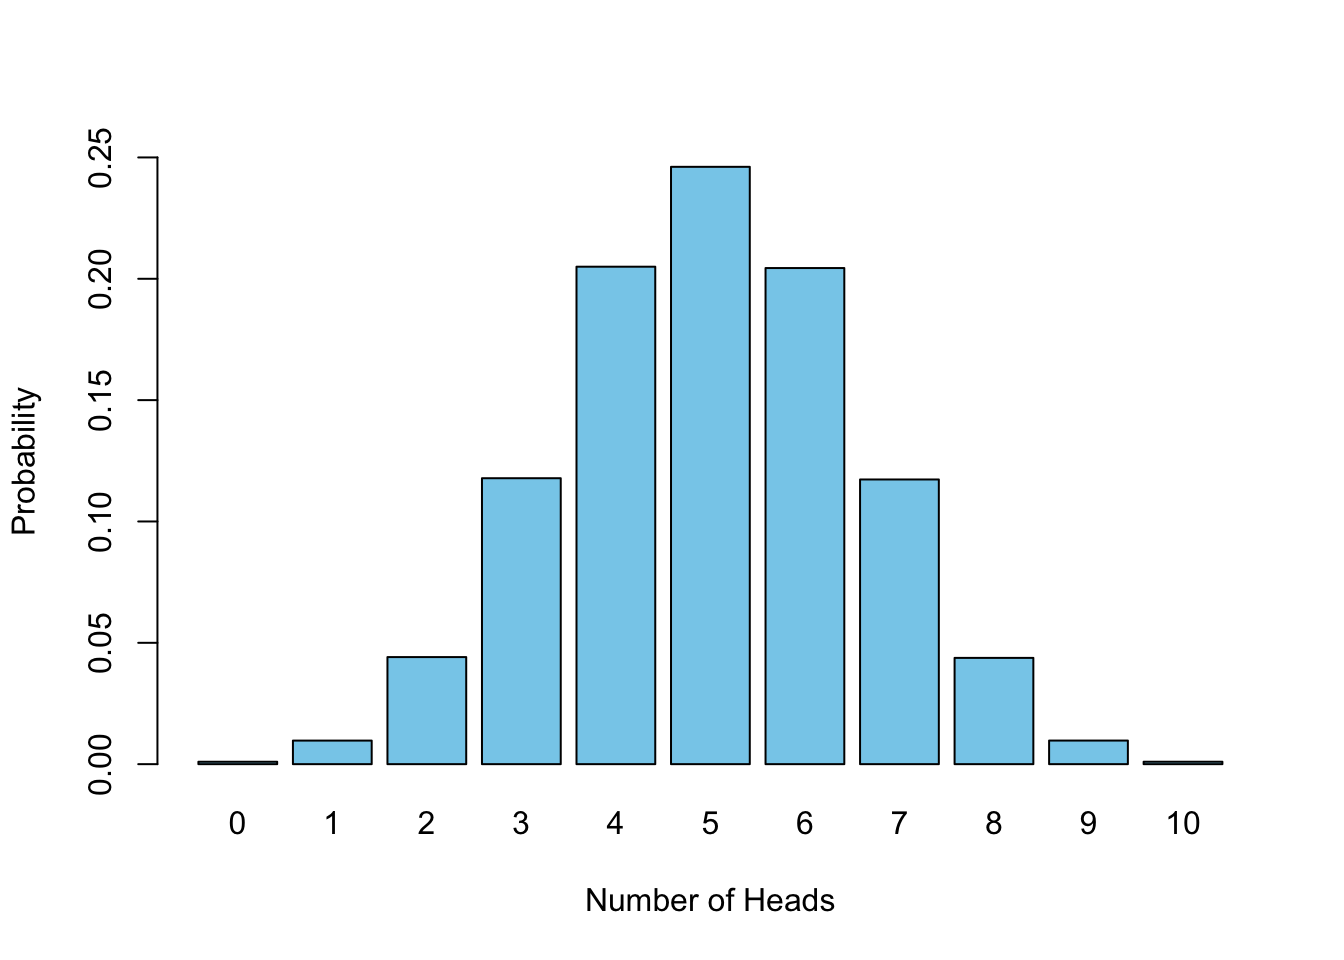
\includegraphics{Research-Design---Statistics_files/figure-latex/c6c5-1.pdf}
\caption{\label{fig:c6c5}Probability distribution of the number of heads out of 10 when repeating the sampling process one million times.}
\end{figure}

I like the graphical view. You can clearly see that getting five heads out of 10 is the most common outcome, but note that this outcome only happens about 25\% of the time. About 75\% of the trials result in an outcome other than five. If we didn't truly know we had a fair coin and we were estimating the probaiblity of heads by flipping the coin 10 times, there would be a difference between our estimate and the true value 75\% of the time. In other words, our estimates are just that - \textbf{estimates}. There is always uncertainty about the quality of an estimate, or how close it is to the truth.

Statistics is fundamentally about how to use data to estimate quantities of interest from samples \textbf{and the uncertainty about those estimates}. If I take a sample of 100 statistics courses and and 20\% of the students in those courses are biology majors, I can't conclude with certainty that the proportion of biology majors is really 0.2. The essential goal of statistics is to not only estimate a quantity of interest from data, but to also estimate the uncertainty about the estimate. We will examine tools that allow us to describe our confidence about the quantities we're trying to estimate. The true proportion of biology majors is very unlikely to be exactly 0.2, but I might be quite confident that it's between 0.15 and 0.25. How confident? Stay tuned.

One of the most significant challenges as scientist faces is how to make decisions about hypotheses in light of uncertainty. Let's say you take a sample of individuals to study the relationship between screen time and cognitive performance in kids, and you find that the kids who spend more time on screens tend to show lower cognitive performance. In your analysis of the data from this study, there is some quantity, or set of quantities, that you have estimated from the sample that indicates this negative association. How certain are you about those estimates? If your estimates are highly uncertain, then your ability to make a firm conclusion about the research question and hypotheses is going to be limited. But better to know about that limitation than to ignore it! Ultimately statistics helps us make decisions about hypotheses with data in light of uncertainty, and I hope to illustrate that idea throughout the book.

\section{Parameters and estimates and estimands, oh my!}\label{parameters-and-estimates-and-estimands-oh-my}

Like most technical disciplines, statistics is full of jargon. Sorry. Let's define some key terms related to sampling. Statistical analysis involves estimating the unknown from sample data. Consider again my goal of estimating the proportion of students in statistics classes that are biology majors. That proportion is unknown. Quantities with unknown values are called \textbf{parameters}. In my example, the parameter is the true proportion of statistics students majoring in biology. The parameter is a probability in this case, but parameters can be means, variances, rates, components of a complex statistical model, or any number of other quantities. The defining feature of parameters is that they are unknown and require estimation to answer your research question. If I collect data on 1000 statistics students and find that 123 are biology majors, then my \textbf{estimate} is 123/1000 = 0.123 for the proportion majoring in biology. Much of this class is about generating estimates (and characterizing their uncertainty) for parameters based on data we collect from samples.

Now, sometimes we have to estimate multiple parameters in a statistical analysis, but not all of the parameters are of direct interest for our research question. The quantities of interest for our reserach question are called \textbf{estimands} \footnote{See \href{https://journals.sagepub.com/doi/abs/10.1177/00031224211004187?journalCode=asra}{Lundberg et al.~2021} for an excellent overview of estimands.}. In my example on the proportion of students majoring biology, the question and analysis is so simple that there's only a single parameter, and it's the parameter I'm interested in. The true proportion of statistics students majoring in biology is the estimand. In a more complex statistical analyses, we will often have to estimate multiple parameters, but not every parameter is of interest. In other words, not every parameter is an estimand. For example, suppose I'm interested in how the amount of time students spend studying affects their grade on an exam. To address a question like that, we could build a regression model - which we will cover in this book - that includes many parameters, but only one of those parameters might be the estimand, representing the causal effect of study time on exam grades. In these cases of complex statistical analyses, it will be important to identify which parameters you're estimating are estimands, which is ultimately based on your research question.

When we estimate quantities from a sample, there's uncertainty about the quality of that estimate - how consistent it is, and how close to the truth it is. Fortunately there are ways to characterize the quality of our estimates and to estimate the uncertainty we have about our estimates. We'll look at different ways of characterizing the quality of an estimate first.

\section{Quality of estimates: accuracy and precision}\label{quality-of-estimates-accuracy-and-precision}

When we estimate quantities from a sample, there's uncertainty about the quantity of that estimate. We will explore two different ways of characterizing the quality of an estimate: how close our estimate should be to the truth based on our sampling design, and the variation in the possible values of the estimate we might obtain based on our sampling design. These two concepts are referred to as \textbf{accuracy} and \textbf{precision}, and estimates are of highest quality when they are both accurate and precise. Let's break these terms down.

\subsection{Accuracy}\label{accuracy}

On average, how close is an estimate from the truth? Let's reconsider our coin flipping problem to estimate the probability of heads. In this case we know we have a fair coin, and so the probaiblity of heads is 0.5, but imagine we didn't know that. Our sampling process consisted of flipping a coin 10 times and recording the number of heads. In this case, the parameter (and estimand) is the true probability of heads, and the estimate is the probability of heads computed from our sample data. If we record 8 heads out of 10 flips, our estimate for the probability of heads is 8/10 = 0.8. On its face, that particular estimate doesn't appear to be very accurate. The estimate is too high. However, take another look at the entire distribution of possible outcomes when we flip a coin 10 times, which we created with a simulation. Let's express the distribution on the scale of probability for the outcome, rather than the number of heads out of 10 (\ref{fig:c6c6}.

\begin{Shaded}
\begin{Highlighting}[]
\NormalTok{possible.estimates }\OtherTok{\textless{}{-}} \FunctionTok{seq}\NormalTok{(}\DecValTok{0}\NormalTok{, }\DecValTok{1}\NormalTok{, }\AttributeTok{by =} \FloatTok{0.1}\NormalTok{)}
\FunctionTok{barplot}\NormalTok{(}\FunctionTok{prop.table}\NormalTok{(}\FunctionTok{table}\NormalTok{(heads)),}
        \AttributeTok{names.arg =}\NormalTok{ possible.estimates,}
        \AttributeTok{ylim=}\FunctionTok{c}\NormalTok{(}\DecValTok{0}\NormalTok{, }\FloatTok{0.28}\NormalTok{),}
        \AttributeTok{xlab =} \StringTok{"Estimated probability of heads"}\NormalTok{, }\AttributeTok{ylab =} \StringTok{"Probability"}\NormalTok{,}
        \AttributeTok{main =} \StringTok{""}\NormalTok{,}
        \AttributeTok{col =} \FunctionTok{c}\NormalTok{(}\FunctionTok{rep}\NormalTok{(}\StringTok{"gray"}\NormalTok{, }\DecValTok{5}\NormalTok{), }\StringTok{"skyblue"}\NormalTok{, }\FunctionTok{rep}\NormalTok{(}\StringTok{"gray"}\NormalTok{, }\DecValTok{5}\NormalTok{)))}
\end{Highlighting}
\end{Shaded}

\begin{figure}
\centering
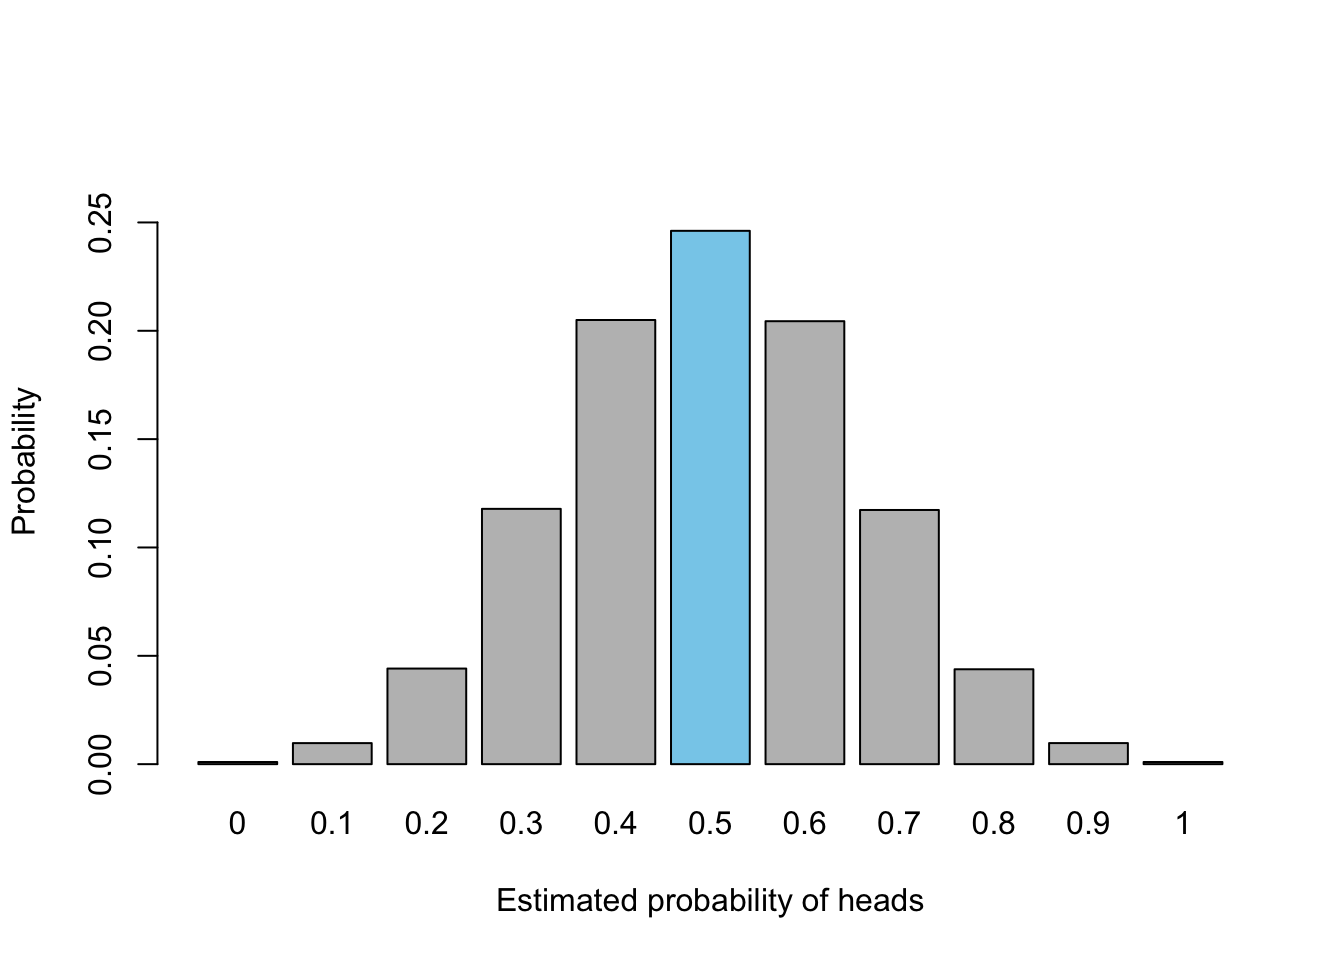
\includegraphics{Research-Design---Statistics_files/figure-latex/c6c6-1.pdf}
\caption{\label{fig:c6c6}Sampling distribution showing accuracy of estimates.}
\end{figure}

Notice that the most likely outcome based on our sampling process is 0.5 (highlighted in blue), which is exactly what the truth is. In other words, when considering our sampling process, repeatedly conducted many times, we get a sense for the entire distribution of possible estimates, and we see that our estimate is - \emph{on average} - accurate. Any particular estimate can be low or high, but there is no systematic difference between the estimate and the truth.

This distribution of possible outcomes of an estimate based on our sampling process is called a \textbf{sampling distribution}. If the sampling distribution is centered on the true value of a parameter, then your estimates are accurate. Figure \ref{fig:c6c7} shows one example of what a sampling distribution might look like when your estimate is not accurate:

\begin{Shaded}
\begin{Highlighting}[]
\DocumentationTok{\#\# generate a biased sampling distribution}
\NormalTok{heads.biased }\OtherTok{\textless{}{-}} \FunctionTok{rbinom}\NormalTok{(}\AttributeTok{n =} \DecValTok{1000000}\NormalTok{, }\AttributeTok{size =} \DecValTok{10}\NormalTok{, }\AttributeTok{prob =} \FloatTok{0.3}\NormalTok{)}
      
\NormalTok{possible.estimates }\OtherTok{\textless{}{-}} \FunctionTok{seq}\NormalTok{(}\DecValTok{0}\NormalTok{, }\DecValTok{1}\NormalTok{, }\AttributeTok{by =} \FloatTok{0.1}\NormalTok{)}
\FunctionTok{barplot}\NormalTok{(}\FunctionTok{prop.table}\NormalTok{(}\FunctionTok{table}\NormalTok{(heads.biased)),}
        \AttributeTok{names.arg =}\NormalTok{ possible.estimates,}
        \AttributeTok{ylim=}\FunctionTok{c}\NormalTok{(}\DecValTok{0}\NormalTok{, }\FloatTok{0.28}\NormalTok{),}
        \AttributeTok{xlab =} \StringTok{"Estimated probability of heads"}\NormalTok{, }\AttributeTok{ylab =} \StringTok{"Probability"}\NormalTok{,}
        \AttributeTok{main =} \StringTok{""}\NormalTok{,}
        \AttributeTok{col =} \FunctionTok{c}\NormalTok{(}\FunctionTok{rep}\NormalTok{(}\StringTok{"gray"}\NormalTok{, }\DecValTok{5}\NormalTok{), }\StringTok{"skyblue"}\NormalTok{, }\FunctionTok{rep}\NormalTok{(}\StringTok{"gray"}\NormalTok{, }\DecValTok{5}\NormalTok{)))}
\end{Highlighting}
\end{Shaded}

\begin{figure}
\centering
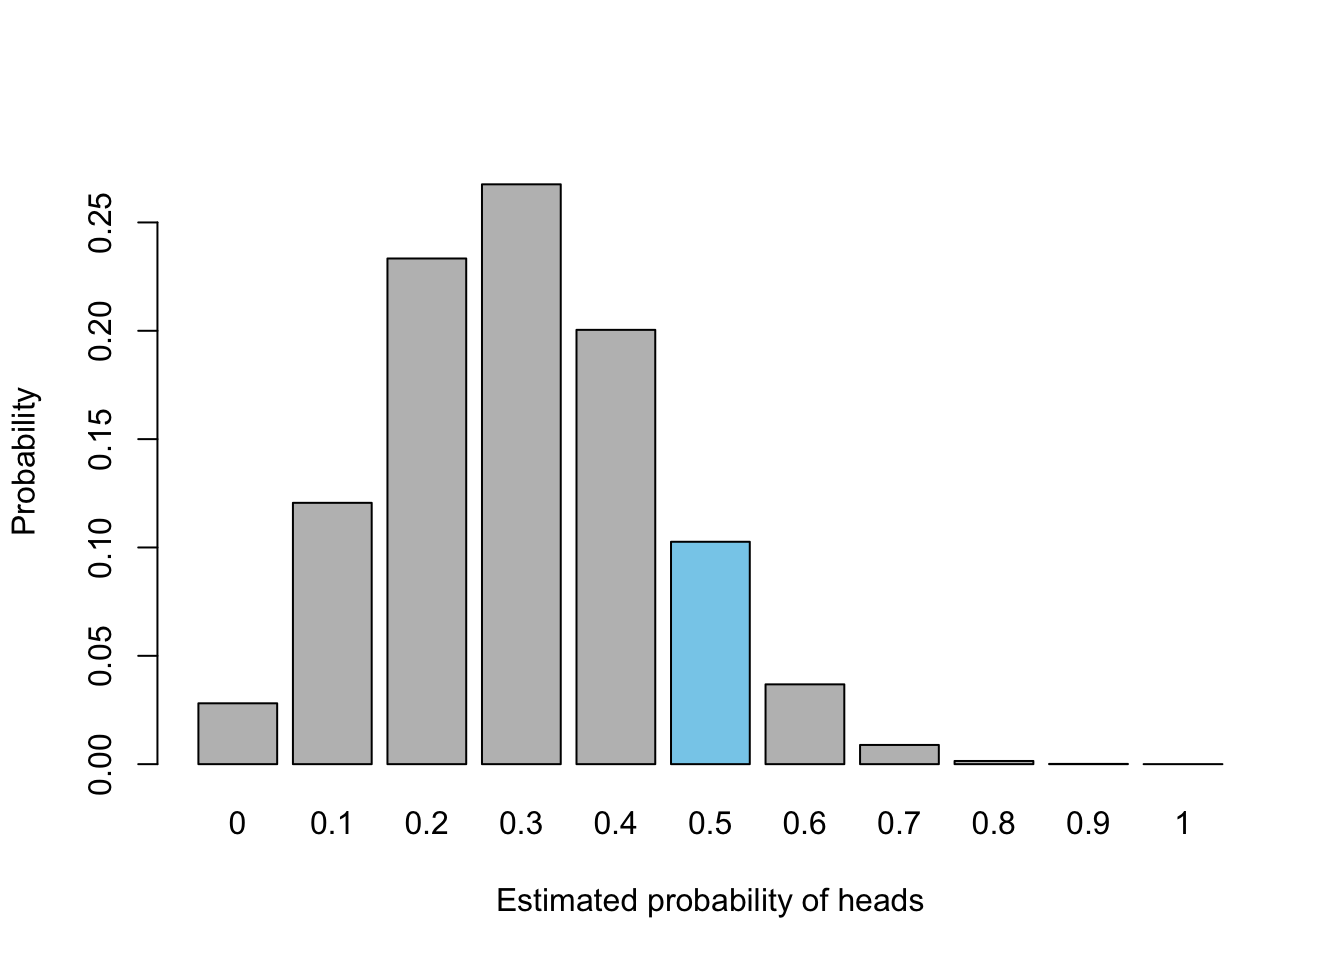
\includegraphics{Research-Design---Statistics_files/figure-latex/c6c7-1.pdf}
\caption{\label{fig:c6c7}Example of a sampling distribution showing biased estimates.}
\end{figure}

Here we can see there's a clear problem in our sampling process. There's variation in the possible estimates just like the first case, but notice that the estimates are more consistently underestimates than overestimates. On average, our estimates are much too low. If the estimates tend to systematically differ from the truth, then the estimates are \textbf{\emph{biased}}. Bias is a consistent discrepancy between the estimates and the true value of the parameter. Estimates may be biased high or biased low (e.g., estimates of 0.20, 0.19, 0.39, 0.32, 0.25, 0.29). When we design a study and sampling process, it is important to use strategies to maximize accuracy (minimize bias). More on that in a bit.

\subsection{Precision}\label{precision}

When we examine the range of possible estimates based on a sampling design, we can examine how much variation we expect to see in the estimates from sample to sample. Consider again the coin flipping sampling process to estimate the probability of heads. When we repeatedly flip a coin 10 times, we know our estimates of the probability of heads will vary because the outcome of each coin flip has an element of chance. Sometimes you end up with 6 heads, other times you get 3 heads. We encounter the sample kind of problem when we sample from any population. Consider again the goal of estimating the proportion of statistics students majoring in biology. If I sample 1000 students, some imprecision is guaranteed because the exact composition of any particular sample of 1000 students is likely to vary just by chance. This chance variation is called \textbf{\emph{sampling error}}, and it leads to some variation in estimates from sample to sample, which we call \textbf{precision}. Precision is a measure of how consistent estimates should be when we repeatedly sample from a population, using the same sampling methodology each time. If the estimates are consistently around the same value, then the estimates are precise. If the estimates vary wildly, then the estimates are imprecise.

From a coarse perspective, we can gauge the precision of an estimate by examining the width of a sampling distribution. Let's visit the coin flipping problem. I've generated two sampling distributions, one where we count the number of heads out of 10 coin flips, and another where we count the number of heads out of 100 coin flips. Each sampling process is repeated 1 million times, and the sampling distributions show the variation in estimates of the probability of heads (Figure \ref{fig:c6c8}. What do you notice that's different between these sampling distributions?

\begin{figure}
\centering
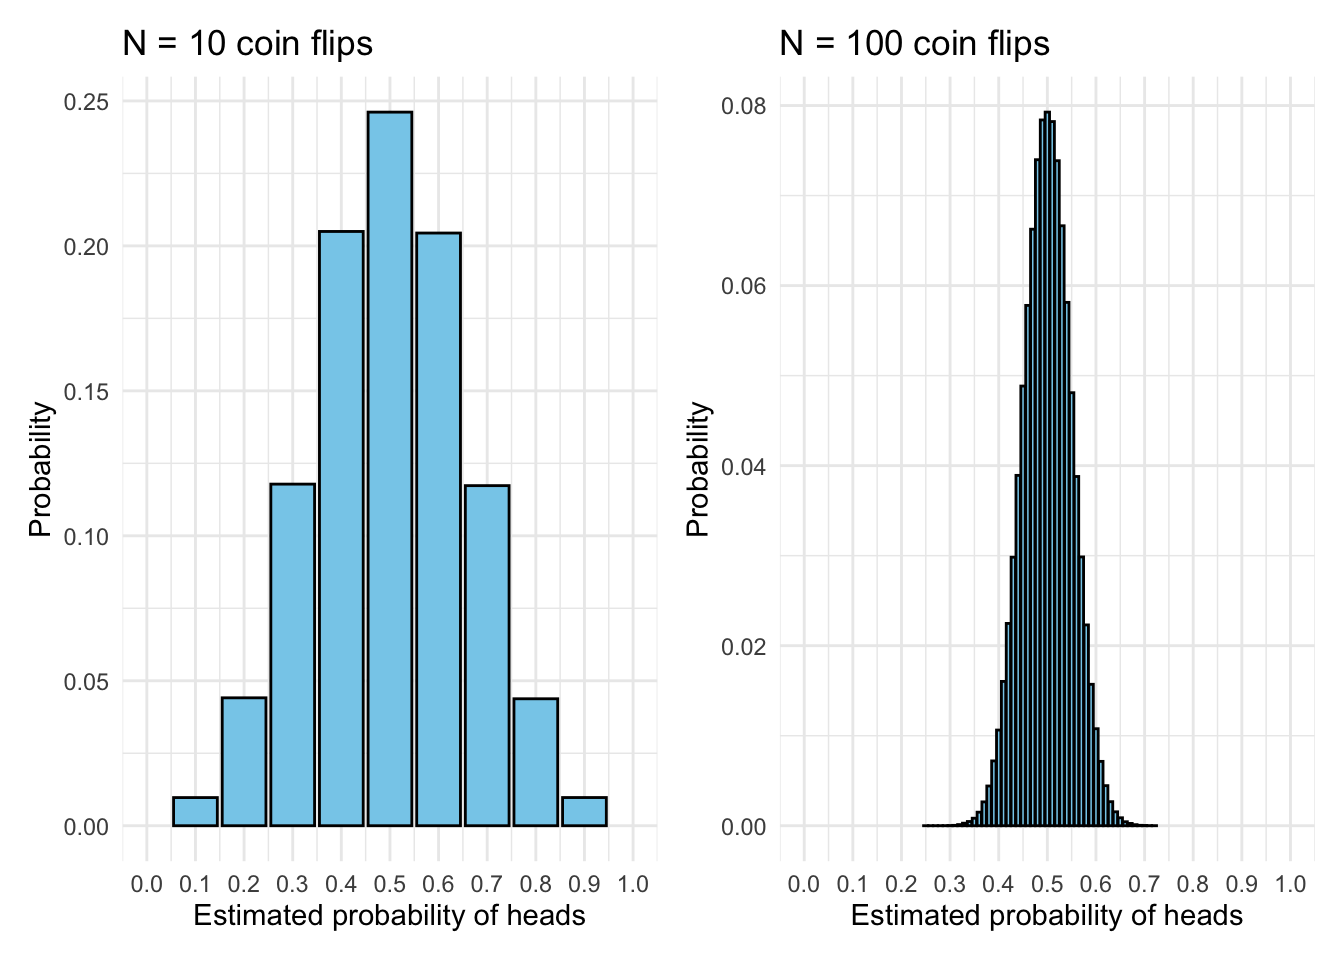
\includegraphics{Research-Design---Statistics_files/figure-latex/c6c8-1.pdf}
\caption{\label{fig:c6c8}Sampling distributions for estimates of the probability of heads based on samples of size 10 (left) vs.~100 (right).}
\end{figure}

These sampling distributions differ in a couple important ways. First, notice that the sampling distribution for N = 10 coin flips is wider than the sampling distribution for N = 100. This is a clear difference in precision between the two sampling approaches. Sampling with N = 10 coin flips leads to less precise estimates of the probability of heads than sampling with N = 100 coin flips. With fewer coin flips, you should expect to see much more variation in the potential estimates. Second, notice that the y-axis scales are different. The most probable outcome under either sampling approach is 0.5 for the probability of heads, but the probability of getting \textbf{exactly} 0.5 as an estimate is much lower when flipping a coin 100 times than when flipping it 10 times. This is simply a consequence of there being many more possible values that you can get for the probability of heads when you flip the coin 100 times. For example, you can get 51/100 = 0.51 for hte probability heads when flipping 100 times, but it's impossible to get 0.51 when you flip a coin just 10 times.

Breaking down the code

Figure \ref{fig:c6c8} shows two sampling distributions for the estimated probability of heads when flipping a coin 10 times vs.~100 times, repeating the sampling process in each case one million times. The simulated data are stored in the objects \texttt{sample10} and \texttt{sample100}. Nothing new there. What's new is that I use the \texttt{dplyr} and \texttt{ggplot2} packages to create a figure of the sampling distributions.

The \texttt{dplyr} package here is used to create a data frame of the possible estimates of the probability of heads \texttt{prob}, the number of times each outcome was observed \texttt{n}, and the computed probability of each outcome \texttt{probabilility}. This is done in two steps. The first step was to initialize the dataframe (\texttt{df10} and \texttt{df100} with the possible values of the probability of heads, \texttt{prob}). Next, the \texttt{dplyr} function was used to computer the observed number of outcomes (\texttt{n}) and probability of each (\texttt{probability}), conveniently adding them to the data frame using the pipe operator, \texttt{\%\textgreater{}\%}. The pipe operator takes the output of one function and passes it as the first argument of the subsequent function, helping to create a sequence of operations that are easier to follow. So in this case, the pipe operator helps create a dataframe of of possible probabilities of heads, observed count of outcomes , and the observed probability of each. The \texttt{mutate} function is used to create a new column in a dataframe based on existing variables, and here is used to quantify the observed probability of each outcome.

The \texttt{ggplot2} package is used to plot the resulting sampling distributions, usingan approach similar to \texttt{dplyr} with a \texttt{+} operator to combine multiple operations to create a graph in one go. The \texttt{ggplot} function initializes the figure with the dataset (\texttt{df10} or \texttt{df100}, assigning \texttt{prob} to the x-axis and \texttt{probability} to the y-axis). The next operation after the \texttt{+} operator is performed by the \texttt{geom\_bar} function, which creates a bar chart. The \texttt{stat\ =\ identity} argument tells \texttt{ggplot2} to make the heights of the bars from the \texttt{probability} column. The following operations are used to adjust the x-axis limits (\texttt{scale\_x\_continuous}) and add labels (\texttt{labs}). The default background theme for \texttt{ggplot2} has gray shading, and I'm not a fan of that, so I add one more operation to add a minimal theme that removes the gray shading.

Note that each figure is assigned a name, \texttt{p1} and \texttt{p2}. The code \texttt{p1\ +\ p2} is executed, which uses the \texttt{patchwork} library to arrange \texttt{ggplot2} figures in a multipanel plot.

I know this is a lot. I'm not a frequent user of \texttt{ggplot2}, but for some types of graphing situations it can be quite handy. Use the exmaples and help documentation to your advantage.

\section{Maximizing accuracy and precision of estimates}\label{maximizing-accuracy-and-precision-of-estimates}

High quality estimates are both accurate and precise. When designing a scientific study, it is critical to design the data collection scheme in a way that will maximize accuracy and precision. Let's go over some attributes of study design that affect accuracy and precision.

\subsection{Random sampling}\label{random-sampling}

The most effective strategy to minimize bias is to take a \textbf{\emph{random sample}} of individuals from the population of interest. A random sample means that every individual in the population has an equal chance of being included in the sample. For our study of sunscreen and skin cancer, the best approach is to identify people in the population of interest, and then randomly sample a subset of those individuals for inclusion in the study. Of course that's easier said than done.

When working with people, it's often difficult to obtain a perfectly random sample, but it's better to be aware of potentially biases in a sample than to ignore them. Consider again the sample of patients to estimate the relationship between sunscreen and skin cancer. Those patient records were simply easy to access, so the individuals in the study were a \textbf{\emph{sample of convenience}}. This is less than ideal because samples of convenience are typically not representative of the broader population of interest. Patients are typically more likely to visit the doctor if they have a problem to begin with, so one concern is that we may be overestimating the prevalence of skin cancer. Conversely, what if the people most likely to visit the doctor also tend to be proactive about their health? Perhaps the people who are more inclined to visit the doctor are more likely to use sunscreen. If the patients most likely to visit the doctor are ones who tend to use sunscreen and tend to visit the doctor because of a symptom, then we might find skin cancer is more prevalent among sunscreen users, an inaccurate conclusion. Samples of convenience often cause bias.

Bias in estimates is similarly caused by \textbf{\emph{volunteer samples}}. The classic case is survey design. Suppose small town is debating about purchasing land to build a park for recreation. The park will include a playground, a splash pad, fields for soccer, baseball, and football, and some tennis courts. The tennis courts and fields will all have lights, allowing people to play in the evenings. The town board wants to see if residents support the idea of building the new park, so they create a survey and mail it to residents. Who's most likely to respond? In this case, volunteer bias would occur if the people most likely to respond are ones who have very strong opinions. For example, residents who are really passionate about having recreation fields may be most likely to respond, causing an overestimate in the proportion of residents who favor creating the park. Conversely, imagine there's a large neighborhood next to the land being considered for purchase, and those residents don't want bright lights on at night in their backyard. Support for the park may be underestimated if the residents in that neighborhood are more inclined to respond to the survey.

\textbf{Important note}: Random sampling is not the same as randomization in an experiment. When we refer to random sampling, we're talking about how individuals are selected from the broader population to participate in a study. Randomization refers to the random assignment of individuals to treatments once they are enrolled in the study.

\subsection{Replication}\label{replication}

The clearest way to maximize precision (i.e., minimize sampling error) is to maximize replication, the number of independent sampling units in a study. The number of indepenent sampling units is also referred to as the \textbf{\emph{sample size}}. Remember that sampling error is the chance variation in estimates due to sampling only a subset of indidivudals from a population. If you could include all individuals from the population in your study, there would be no sampling error. Sampling error decreases as you increase the sample size. We proved this to ourselves with the coin flipping example. There was much more variation in estimates of the probability of heads when flipping a coin 10 times than when flipping a coin 100 times. If you increase the sample size to even greater than 100 coin flips, the estimates will be much more precise.

Note that I defined replication as ``the number of \textbf{independent} sampling units. Independence is really important, because it affects how you count sampling units and ultimately determine the sample size in a study. Replicates are independent if the measurements from one replicate have no influence on the measurements from other replicates. Sometimes individuals in a study are not independent. For example, consider again the survey about building a park. Should the researcher include multiple people from the same household in the survey? They certainly could, but the responses of individuals from the same household are likely correlated. In other words, individuals from the same household may have similar preferences about the park. If you included these individuals in your study and counted them as independent replicates, your estimates will be less precise than you think. Counting individuals as unique replicates when they are not independent is referred to as \textbf{\emph{pseudoreplication}} and can lead to incorrect inferences. More on that later!

\textbf{Important note}: Sample size affects precision, but it does not affect accuracy of estimates. Remember that accuracy is how close, \textbf{on average}, your sample estimates are to the true value of the parameter. There's no inherent effect of sample size on accuracy. In other words, low sample size does not cause bias. Consider the coin tossing example. Estimates of the probability of heads varied quite a bit more when using sample sizes of 10 flips rather than 100 flips. In other words, the estimate are less precise with a sample size of 10. But using 10 flips did not introduce bias (i.e., a consistent underestimation or overestimation of the probability of heads). Both sampling distributions are centered on the true probability of heads, 0.5.

\section{Study design elements specific to experiments}\label{study-design-elements-specific-to-experiments}

Random sampling and high replication are arguably the two most important properties of good samples in that they are principles that apply to virtually any study, experimental or observational. There are some additional elements of study design that can help maximize accuracy and precision that are particularly relevant in experiments. Let's work through a few.

\subsection{Control groups}\label{control-groups}

Control groups are mainly applicable to experiments where researchers randomly assign individuals to different treatments. Suppose a study is being designed to test the effect of a vaccine on the probability of getting Covid. Researchers enroll 100 people in the study and follow them for two years. In the first year, no one gets the vaccine. In the second year, everyone gets the vaccine. The probability of getting Covid was 15\% in the first year and 5\% in the second year, so a 10\% reduction in the year when the vaccine was administered. Was the reduction in the risk of Covid caused by the vaccine? Unfortunately, it's hard to say because the researchers did not include a control group, a group that does not receive the treatment of interest. Maybe Covid was simply more virulent (more likely to infect people) in the first year than the second year, and virulence of covid strains is confounded with treatment. If that were the case, a control group would also show a reduction in the probability of covid from year one to year 2. Control groups help researchers make accurate inferences about causation by providing a baseline for comparison to the experimental treatment.

Control groups are often considered *\textbf{placebos}, which refers to a fake treatment. Good placebos mimic the process of the actual treatment to the greatest extent possible. For example, the control group in the vaccine study would receive a needle injection just like the treatment group with the vaccine, except the placebo would involve injection of salt water. The treatment and placebo injections should be the same amount of liquid and injected in the same place. Keeping treatment and placebo groups as similar as possible helps to isolate the difference between the treatment and control group directly to the treatment effect of interest (i.e., the vaccine).

\textbf{Important note:} Not every experiment has a control group, per se. Imagine you are studying the effect of different doses of a medication for acid reflux: 10 mg, 20 mg, 30 mg once a day. One does not absolutely need a control group to compare the degree of acid reflux among these treatment groups. A control group \textbf{would} be needed if the researchers wanted to test whether the medication reduces the amount of acid reflux relative to untreated individuals.

\subsection{Control of variation}\label{control-of-variation}

Consider again the study of the effect of medication doses on acid reflux. One important element of experimental design is controlling for sources of variation in the response variable other than the treatment. For example, the researchers wouldn't want some participants to take their 10 mg pill with water and other participants to take the pill with soda, as that could introduce variation in reflux independent of the treatment. Statistically, controlling other sources of variation in an experiment will help increase precision of estimates.

\textbf{Important note:} Controlling variation in an experiment is different than creating a control group.

\subsection{Blocking}\label{blocking}

Sometimes it's difficult to control for strong sources of variation in an experiment. For example, in the study on acid reflux, individuals might vary dramatically in their diet, which can introduce a lot of variation in acid reflux independent of the effect of the medication. In a case like this, researchers might use a \textbf{\emph{blocked design}}, which involes stratifying the participants in the study into different groups, or blocks. In the acid reflux case, individuals could be stratified into groups based on diet (e.g., high acidity vs.~low acidity diet). Once the blocks are defined, the researchers would then randomly assign each of the treamtents to individuals in each block. By assigning each treatment to individuals in each block, one can avoid any confounding between the treatments and the factor being blocked.

\subsection{Blinding}\label{blinding}

Blinding is helpful to avoid bias in experiments. It applies to cases when bias can be introduced by either the experimenter or subjects knowing which treatments were applied to individual subjects. For example, a patient who knows they received a vaccine treatment might behave differently than a patient who knows they received a placebo. Maybe the patient who knows they received the vaccine will be more inclined to spend time indoors in crowded spaces when Covid is circulating widely, which may increase their risk of getting covid. To minimize this kind of bias, patients are often blinded to the treatment they receive. Experimenters sometimes need to be blinded too. For the study on acid reflux, suppose a laryngologist is quantifying the degree of reflux in each patient by scoring the amount of redness in the larynx upon examination. If the laryngologist knows a patient received the maximum dose, they may be more skeptical about recording very high values of redness given that the expected effect of the drug is to reduce reflux. To avoid this bias, individuals who make observations of experimental subjects are often blinded from knowing the treatment the subject received.

\chapter{Probability}\label{probability}

One of the central goals of epidemiology is to monitor and understand the prevalence of disease. Basic information on the prevalence of disease is used by public health officials to guide decision-making on interventions. Perhaps there's no better example of this than the Covid-19 pandemic that started in late 2019 and led to dramatic measures intended to reduce the spread of the virus, such as social distancing, mask wearing, travel restrictions, school shutdowns, and quarantine. These interventions place significant limitations on the freedoms that we tend to take for granted, and so the benefits of these measures to the public must outweigh the costs.

In this chapter, we will use a simplified version of monitoring disease prevalence to explore concepts about \emph{probability}. Here's the scenario. Imagine you're the lead epidemiologist in a local community of 10,000 people working with public health officials to make decisions about interventions to minimize the spread of a new viral disease. Based on a cost-benefit analysis, public officials have determined that interventions will be enforced if the prevalence of the disease reaches a 10\% threshold. As the lead epidemiologist, your primary goal is to estimate the prevalence of the disease by testing individuals. For now we will assume the test is fool proof. When someone has the virus, the test is always positive, and when someone doesn't have the virus, the test is always negative.

You don't have the time or resources to test everyone, so you plan to sample individuals from the broader population for testing. You know now that random sampling is necessary to ensure accurate estimates, and although true random sampling in public health is hard to do, we'll assume you can select individuals randomly for the sake of this example.

You also know that when you estimate a quantity of interest, there is inevitably \textbf{uncertainty} about the estimate due to sampling error. This is the ultimate reason why we need rigorous statistical methods. When we sample from populations, we cannot answer questions with certainty. There is some true, but unknown proportion of people in the community infected with the virus. Your estimate will be burdended with \textbf{uncertainty}, and in order to evaluate the quality of your estimate, we have to work towards quantifying uncertainty, and we do that in terms of probability.

\section{Defining probability}\label{defining-probability}

Let's start with some terms. When we test an individual for infection, the test is called a \emph{trial}. A trial is simply any process that produces a probabilistic \emph{outcome}. There are only two possible outcomes of the test: positive or negative. These outcomes are \textbf{mutually exclusive}, meaning that an individual cannot test positive \emph{and} negative for the infection at the same time. The set of all possible mutually exclusive outcomes is called the \emph{sample space}. The sample space is often denoted \(\Omega\) and defined in brackets. For example, the sample space for infection status is \(\Omega\) = \{positive, negative\}.

When examining a probability, we are interested in the probability of a particular \emph{event} that we a define. The event could be as simple as the occurrence of a single outcome, such as an individual testing positive. But events can also be defined as sets of outcomes. For example, consider tossing a six-sided die, where the sample space is \(\Omega\) = \{1,2,3,4,5,6\}. Here we could define the event as rolling an even number, which includes three of the possible outcomes.

Ultimately probability is a parameter with a numerical value between 0 and 1. It is variably abbreviated as \emph{p} or \emph{P}, but the event of interest is usually appended. For example, we can define the probability of the event of interest ``X'' as \(p_{X}\) or \(P(X)\). In our example, we're interested in the probability of infection, which we can denote \(p_{infected}\) or \(P(infected)\). I will use both of these naming conventions at times throughout the book.

The quantitative definition of probability is pretty straightforward. But philosophically, what does probably actually mean? It turns out there are multiple interpretations of probabilities. Let's take a look at the two most common interpretations:

\subsection{Frequentist definition}\label{frequentist-definition}

The \textbf{frequentist} definition of probability is one you are probably already familiar with: probability is the proportion of trials \emph{n} where we observe the event of interest, \(X\):

\[
P(X) = \frac{X}{n}
\]

Let's just assume for now that of the 10,000 people in the community, 500 are infected with the virus. Under the frequentist definition, the probability of the infection (\(I\)) is

\[
P(I) = \frac{I}{n} = \frac{500}{10000}=0.05
\]

The frequentist definition simply looks at the frequency of the event of interest relative to the total number of trials. A probability is a proportion, thus constrained to values between 0 (where the event of interest does not occur) and 1 (where the event of interest is a certainty). Probabilities can also be expressed as percentages. To do this, simply multiply the proportion by 100. Saying the probability of infection is 0.05 is the same as saying 5\% of the population is infected.

Now in practice, how do we know the frequentist probability? As the formula implies, we could go track down all \(n\) individuals in the population and give them our fool proof test for the viral infection. But you know that tracking down every individual in the population is usually not feasible, so we usually need to estimate the probability of interest with a sample of data. For example, imagine you randomly sample \(n = 15\) individuals and find one of the 15 tests are positive. In this case, the estimated probability of infection (\(\hat{p}\)) is

\[
\hat{p}_{infected} = \frac{I}{n} = \frac{1}{15}=0.067
\]

Remember that the carrot symbol simply indicates that our quantity is an estimate based on a sample.

There is a way of logically deriving true frequentist probabilities, but this approach is restricted to only the most simple of examples, such as tossing a coin or rolling a die, where you can count the number of times the event of interest occurs out of the sample space. When we flip a coin, there are two sides, heads and tails. Assuming we have a fair coin and flip, the probability of heads must be 0.5, because heads represents half of the sample space. Similarly, if we roll a four-sided die with the numbers 1, 2, 3, and 4, the probability of seeing a ``four'' must be 0.25, because four represents one out of four possible outcomes.

Why doesn't this logic of deriving frequentist probability mathematically work when applied to our viral test? After all, each individual is infected or not infected. In this limited sample space, infected represents one of two possible outcomes, so isn't the probability of infection 0.5? No! When we derive the probability of heads when flipping a coin, or the probabity of rolling a \emph{4} on a four-sided dice, it is important to note that we made important assumptions. We assumed we have fair coin flips and fair dice, and we assumed coin flips and dice tossing is conducted in a random way. In other words, deriving probabilities mathematically from the sample space inevitably requires assumptions about the external forces that can affect the probability of heads, or the probability of rolling a four. If I do not give the coin a fair toss, for example by just dropping the coin flat with the heads face up, then the probability of heads will very likely \emph{not} be 0.5. There are a multitude of external forces that affect the likelihood of an individual being infected with a virus, such as exposure, immune function, public health measures, and even the prevalence of the infection itself.

\subsection{Bayesian definition}\label{bayesian-definition}

The \textbf{Bayesian} way of thinking about probability is as a strength of belief. What do you believe is the probability of infection? We make these kind of subjective probability assessments all the time. If you look outside and see storm clouds on the horizon, you might be inclined to believe it's more likely than not that it will rain today. When you are deciding which route to take to work, you might notice it's the middle of rush hour and conclude there's a 90\% chance that you'll end up in stop-and-go traffic on the interstate. When watching your favorite college basketball team take on the \#1 ranked team, you might conclude your team has only a 10\% chance of winning.

These subjective beliefs aren't empirically computed by frequencies across multiple trials. Rather, they are subjectively computed in your mind based on your knowledge, experience, and intuitions. If you've never heard of anyone being infected with the viral infection being investigated, you might be inclined to conclude it's more likely than not that the prevalence of the virus is below 10\%. In this case you're assigning a subjective probability statement (\textgreater50\% strength of belief) about the frequentist value of a probability (the proportion of individuals infected being below 10\%).

In \href{https://sites.google.com/site/doingbayesiandataanalysis/}{\emph{Doing Bayesian Data Analysis}}, the author John Kruschke talks about how subjective beliefs about probability can be calibrated by comparing those beliefs with events that have known probabilities. For example, suppose I offer you two choices. You can win \$20 if you flip a coin and the result is heads, or you can win \$20 if your favorite college basketball team beats the \#1 ranked team. If you choose the coin flip, you are implicitly concluding that the probability of your team winning is less than 50\%.

Now, Bayesian probabilities aren't always completely subjective. Indeed, much of Bayesian data analysis that we will encounter in the book involves updating our subjective beliefs about a probability (which we will call a \emph{prior probability}) with frequentist probabilities informed by data that we collect. Stay tuned!

\section{Probability rules}\label{probability-rules}

One can take an entire course on the mathematics and theory of probability, but here our goal is to apply some basic knowledge of probability to science and data analysis. That said, familiarity with some basic rules of probability is necessary to do applied statistics. Let's take a look at those rules \footnote{These basic probability rules apply whether you interpret probability based on frequencies of events or strength of belief.}.

Rule 1: The probability of any event X is non-negative.

\[
P(X) \geq 0
\]

Rule 2: The probability of any possible outcome in the sample space \(\Omega\) is certain (1).

\[
P(\Omega) = 1
\]

This rule implies that the probability of all mutually exclusive outcomes must add to 1.

Rule 3: Addition rule

\[
P(A\ \text{or}\ B) = P(A) + P(B)
\]
If outcomes A and B are mutually exclusive, then the probability of either A or B occurring is the sum of their individual probabilities.

Let's apply the addition rule to an example. Consider a six-sided dice with \(\Omega\) = \{1, 2, 3, 4, 5, 6\}. When the dice is rolled, each outcome is mutually exclusive, so we can apply the addition rule to quantify the probability of one event or another. For example, the probability of rolling a ``1'' or ``2'' is.

\[
P(1\ \text{or}\ 2) = P(1) + P(2) = \frac{1}{6}+\frac{1}{6}=0.333
\]
We can extend this rule beyond two events. For example, the probability of a ``1'', ``2'', or ``3'' is

\[
P(1\ \text{or}\ 2\ \text{or}\ 3) = P(1) + P(2) +P(3) = \frac{1}{6}+\frac{1}{6}+\frac{1}{6}=0.5
\]
The first three probability rules above are known as \textbf{Kolmogorov's Axioms of Probability}, named after the Russian mathematician Andrey Kolmogorov. Rules 1 and 2 together imply that probability is mathematically bounded between 0 and 1: \(0 \leq P(X) \leq 1\), and Rule 3 allows us to quantiy the probability of one or more mutually exclusive events. From these three rules, we can derive a fourth rule:

Rule 4: Not rule

\[
P(\text{not}\ A) = 1 - P(A)
\]
The probability of an event not occurring is one minus the probability that it occurs.

For example, when rolling a six-sided dice, the probability of not rolling a ``5'' can be quantified as

\[
P(\text{not}\ 5) = 1 - P(5) =1-\frac{1}{6}=0.833
\]
\#\# Joint events

The first four rules apply to events in isolation, but often we are interested in the joint probability of multiple events occurring at the same time. For this situation let's consider again the goal of estimating the prevalence of a viral infection. The epidemiologist does not know the true prevalence, but let's assume it's 5\%. The epidemiologist randomly samples two people from the population and surprisingly finds that both are infected! What was the probability of two randomly-selected individuals being infected when the prevalence of the infection is 5\%? Here we are interested in a \textbf{joint probability}, namely the probability of the first \emph{and} second individuals being infected.

\subsection{Joint events under independence}\label{joint-events-under-independence}

In cases where the joint events are \textbf{independent}, we can apply the following rule to quantify the joint probability:

Rule 5: Multiplication rule

\[
P(A\ \text{and}\ B) = P(A)P(B)
\]

When events A and B are independent, the probability of A and B is the multiplication of the probabilities of A and B individually.

For events to be independent, one event must have no impact at all on the probability of another event. In the context of testing, this would mean that the infection status of individual A must have no impact on the infection status of individual B. The infection status of both people must be completely unrelated. If that's the case, then we can quantify the probability of individuals A and B both being infected as

\[
P(infected\ and\ infected) = 0.05*0.05=0.0025
\]

When the prevalence of the infection is 5\%, the probability that two randomly-selected individuals will both be infected is only 0.25\%. A rare event indeed!

Consider another example. According to the \href{https://www.pewresearch.org/short-reads/2023/08/15/32-of-americans-have-a-tattoo-including-22-who-have-more-than-one}{Pew Research Center}, approximately 32\% of Americans have a tattoo. Let's assume that's the case in the community of interest. If one individual is selected at random, what is the probability the individual is infected \emph{and} has a tattoo. Assuming these are independent events, the probability can be quantified as

\[
P(infected\ \text{and}\ tattoo) = 0.05*0.32=0.016
\]

\subsection{Joint events under non-independence (conditional probability)}\label{joint-events-under-non-independence-conditional-probability}

Are we making good assumptions? Is the probability of a viral infection really independent of having a tattoo? I doubt there's a direct causal effect of having a tattoo on infection status (or vice-versa), but might there be differences in behavior between people with and without tattoos that could affect infection status? Some pyschological studies have shown that people with tattoos tend to score higher on extraversion than people without tattoos (e.g., \href{https://journals.sagepub.com/doi/abs/10.2466/09.07.21.PR0.111.4.97-106?casa_token=GG6UgmonrdAAAAAA:REJHZeVgnjOn2KVpShnrxHf-9M5QSt-TMPkMgliduw_ZaGClESfJkRM3hYkIlXz5xaWDgCp6B_Nr}{Swami et al.~2012}. If people with tattoos are more open or social and therefore around other more than individuals without tattoos, perhaps people with tattoos will be exposed to a virus more than people without tattoos.

Or what about independence when we sample two individuals for testing? Are the results of those tests really independent? If the individuals were truly selected at random, I suspect the independence assumption holds in that case. But we can imagine cases where the outcomes are not independent. For example, what if the two individuals are in the same household, with largely the same set of exposures (including each other)? That's a fairly clear example where we should not expect the outcomes to be independent.

This is getting interesting! Indeed, non-independence of joint probabilities is, from a very mathematical perspective, at the heart of scientific research questions, particular questions about explanation. Does social behavior affect infection status? Such a question can be addressed quantitatively by examining joint probabilities under assumptions of independence vs.~dependency between the events.

To analyze joint probabilities of multiple events when those events are not independent, we need to define \textbf{conditional probability}. A conditional probability can be defined as the probability of event A given that know event B is true. Let's formalize another rule:

Rule 6: Conditional probability

\[
P(A|B) = \frac{P(A\ \text{and}\ B)}{P(B)}
\]

The vertical bar (\textbar) means ``given'', so \(P(A|B)\) reads ``the probability of A given B''. For example, suppose we know someone has a tattoo. Might that give us some information on whether or not they are infected? Consider Table \ref{tab:c7t1}, which shows simulated data for the number of individuals out of 10,000 with each combination of outcome for infection and tattoo status.

\begin{table}
\centering
\caption{\label{tab:c7t1}<span style='color:black; font-weight:bold;'>Counts of Infection Status vs. Tattoos (N = 10,000)</span>}
\centering
\begin{tabular}[t]{l|r|r|r}
\hline
Status & Tattoo Count & No Tattoo Count & Total Count\\
\hline
Infected & 250 & 250 & 500\\
\hline
Not Infected & 2950 & 6550 & 9500\\
\hline
Total & 3200 & 6800 & 10000\\
\hline
\end{tabular}
\end{table}

Let me point out a couple important things about Table \ref{tab:c7t1}. First, notice that we can see the overall probability of infection is 5\% as we previously assumed. There are 500 total people infected out of 10000. We can also see the overall probability of having a tattoo is 32\%, as 3200 out of 10,000 people have tattoos. These probabilities are called \textbf{marginal probabilities} because we are marginalizing the probabilities across levels of a different variable. In other words, to get the total probability of infection, we have to use the data on infection of both tattooed and non-tattooed people, and to get the probability of tattoo, we have to use the data on tattos for both infected and non-infected people.

Second, from these data we can compute the joint probabilities of each combination of events:

\begin{Shaded}
\begin{Highlighting}[]
\DecValTok{250}\SpecialCharTok{/}\DecValTok{10000} \CommentTok{\#Infected and Tattoo}
\end{Highlighting}
\end{Shaded}

\begin{verbatim}
## [1] 0.025
\end{verbatim}

\begin{Shaded}
\begin{Highlighting}[]
\DecValTok{2950}\SpecialCharTok{/}\DecValTok{10000} \CommentTok{\#Not infected and Tattoo}
\end{Highlighting}
\end{Shaded}

\begin{verbatim}
## [1] 0.295
\end{verbatim}

\begin{Shaded}
\begin{Highlighting}[]
\DecValTok{250}\SpecialCharTok{/}\DecValTok{10000} \CommentTok{\#Infected and No tattoo}
\end{Highlighting}
\end{Shaded}

\begin{verbatim}
## [1] 0.025
\end{verbatim}

\begin{Shaded}
\begin{Highlighting}[]
\DecValTok{6550}\SpecialCharTok{/}\DecValTok{10000} \CommentTok{\#Not infected and No tattoo}
\end{Highlighting}
\end{Shaded}

\begin{verbatim}
## [1] 0.655
\end{verbatim}

The joint probabilities quantify the proportion of individuals in the total population who meet the definition of both events. Out of all the people in the population, the probability of being infected \emph{and} having a tattoo is \(250/10000 = 0.025\). Note that these four combinations consist of the entire sample space for the joint probability of infection status and tattoo status, so these joint probabilities should sum to 1.

OK, now let's get back to the question of conditional probability. Are the events infection status and tattoo status independent? If they are independent events, then the probability of infection shouldn't depend at all on tattoo status. In other words, the prevalence of the infection be the same for each level of tattoo status. Let's see if that's the case, here applying our rule to quantify conditional probabilities:

\[
P(infected|tattoo) = \frac{P(infected\ \text{and}\ tattoo)}{P(tattoo)}=\frac{250}{250+2950}=0.078
\]

\[
P(infected|no\ tattoo) = \frac{P(infected\ and\ no\ tattoo)}{P(tattoo)}=\frac{250}{250+6550}=0.038
\]
Here we clearly see that the probability of infection is 4\% greater for those with tattoos than those without tattoos. In other words, infection status is \emph{not} independent of tattoo status!

How do we compute joint probabilities when events are not independent? There's a rule for that!

Rule 7: General multiplication rule

\[
P(A\ \text{and}\ B) = P(A|B)P(B)
\]

This general multiplication rule is derived from Rule 6 on conditional probability by simply isolating \(P(A\ and\ B)\). As an example, if I told you the overall proportion of those with tattoos was 32\% and the probability of infection among those with tattoos was 7.8\%, you can quantify the overall probability of those with infections and tattoos as

\[
P(infection\ and\ tattoo) = P(infection|tattoo)P(tattoo)=0.078*0.32=0.025
\]

Note that we can show infection status and tattoo status are not independent by testing the simple multiplication rule (Rule 5). The simple multiplication rule says that the joint probability of independent events is the multiplication of their individual probabilities. Thus, if infection status and tattoo status are independent, the proportion of people who are infected and have a tattoo should be \(0.05*0.32=0.016\). But that's not the case! The table above shows that 250 people out of 10,000 have tattoos and are infected. Our simple multiplication rule doesn't work because it assumes independence, and tattoo status and infection status are not independent in this example.

\subsection{One thing or another (general addition rule)}\label{one-thing-or-another-general-addition-rule}

Let's revisit the situation when we want to know the probability of one event \emph{or} another event. When the events are mutually exclusive, the addition rule tells us to simply add the probabilities of each event. What if the events are not mutually exclusive? For example, what if I randomly select and individual and want to know if that person is infected \emph{or} has a tattoo. If we apply the simple addition rule, we would conclude the probability of infection or tattoo is \(0.05 + 0.32 = 0.37\), but that's not correct. Why not? The problem is that some of the infected people have tattoos! If you just add the overall probability of infection and tattoo, you are double counting those people. To quantify the probability of event A or B when A and B are not mutually exclusive, we need to apply the \textbf{general addition rule}:

Rule 8: General addition rule

\[
P(A\ \text{or}\ B) = P(A) + P(B) - P(A\ \text{and}\ B)
\]

Let's apply this to the infection and tattoo example:

\[
P(infection\ \text{or}\ tattoo) = P(infection) + P(tattoo) - P(infection\ \text{and}\ tattoo)=0.05+0.32-0.025=0.345
\]

Having fun yet?

\subsection{Quantifying marginal probabilities}\label{quantifying-marginal-probabilities}

When working with joint events, sometimes we want to work backwards from disaggregated probabilities to aggregated, or marginal probabilities. For example, suppose you knew the probability of infection separately for individuals who have tattoos and those who don't have tattoos. In probabilistic terms, we know \(P(infection|tattoo) = 0.078\) and \(P(infection|no\ tattoo) = 0.038\). What's the overall prevalence of infection? You might be tempted to compute the simple average of 0.078 and 0.038, but the mean (0.058) is not correct. Why not? The mean does not weight the conditions of tattoo status appropriately. We know 32\% of the population has a tattoo, whereas 68\% of the population does not have a tattoo. We need to account for the fact that more of the population does not have tattoos. The mean applies equal weight to both conditions, effectively assuming that half the population has a tattoo.

To quantify the marginal probability of infection (i.e., marginalizing the probability of infection over the levels of tattoo status), we to basically quantify a weighted mean. This is the \emph{law of total probability}:

Rule 9: Law of total probability

\[
P(A) = \sum_{i=1}^n P(A|B_i)P(B_i),
\]

where \(A\) is event A and \(B_i\) is condition \emph{i} of event \(B\).

Here we see the total (marginal) probability of event A is the weighted average of the probability of A across conditions of event B. Now let's apply this rule to quantify the probability of infection across conditions of tattoo status:

\[
P(infected) = P(infected|tattoo)P(tattoo) + P(infected|no\ tattoo)P(no\ tattoo)
\]

\[
P(infected) =0.078*0.32+0.038*0.68=0.05
\]

\section{Sampling and probability distributions}\label{sampling-and-probability-distributions}

Ok, that was a fair amount of pure probability theory. But this isn't a probability book, or a theory book. This is a book about applied research design and statistics. In this section we begin to apply basic probability theory to practical questions about the ultimate goal of statistics: estimating unknown quantities by sampling.

Let's get back to being the lead epidemiologist. Suppose that instead of randomly testing individuals from the entire community, you are focused on one household. This household has four people, two parents and two kids. Each person in the household can be infected or not infected, and you want to figure out \emph{how many people in the household are infected}. With four people in the household and the sample space being infected or not infected, there are five possible outcomes for the number of infected people in the household, ranging from no one being infected to all four family members being infected.

Sadly you only have two test kits available, so you can't test the whole family. You're going to test two people, and to make matters more simple from a probability perspective, you're going to test the family members \textbf{with replacement}. What that means is you are going to randomly conduct two tests, but each person is available to be selected for both tests. This is analogous to randomly selecting multiple playing cards from a deck, but each time replacing the card you chose before you select a new one.

Suppose you go ahead and randomly conduct two tests and find that one of the two tests was positive, and one of the two tests was negative. In probability terms, we know there was \(X = 1\) positive test out of \(n = 2\) trials. What insight do these data provide into the infection status of the entire family?

The way we're going to interrogate this issue is by quantifying the probability of the data we observed under each of the five possibilities for the proportion of the family infected. As an example, let's assume that only one of the family members is truly infected. In other words, \(p_{infected} = 0.25\). If only one of the four family members is infected, how likely were we to see one positive out of two tests? To answer that question, let's look at all the possible outcomes when we conduct two tests, given that only one member is infected. Figure \ref{fig:c7f1} shows these possibilities in the format of a branching tree.

\begin{figure}

{\centering 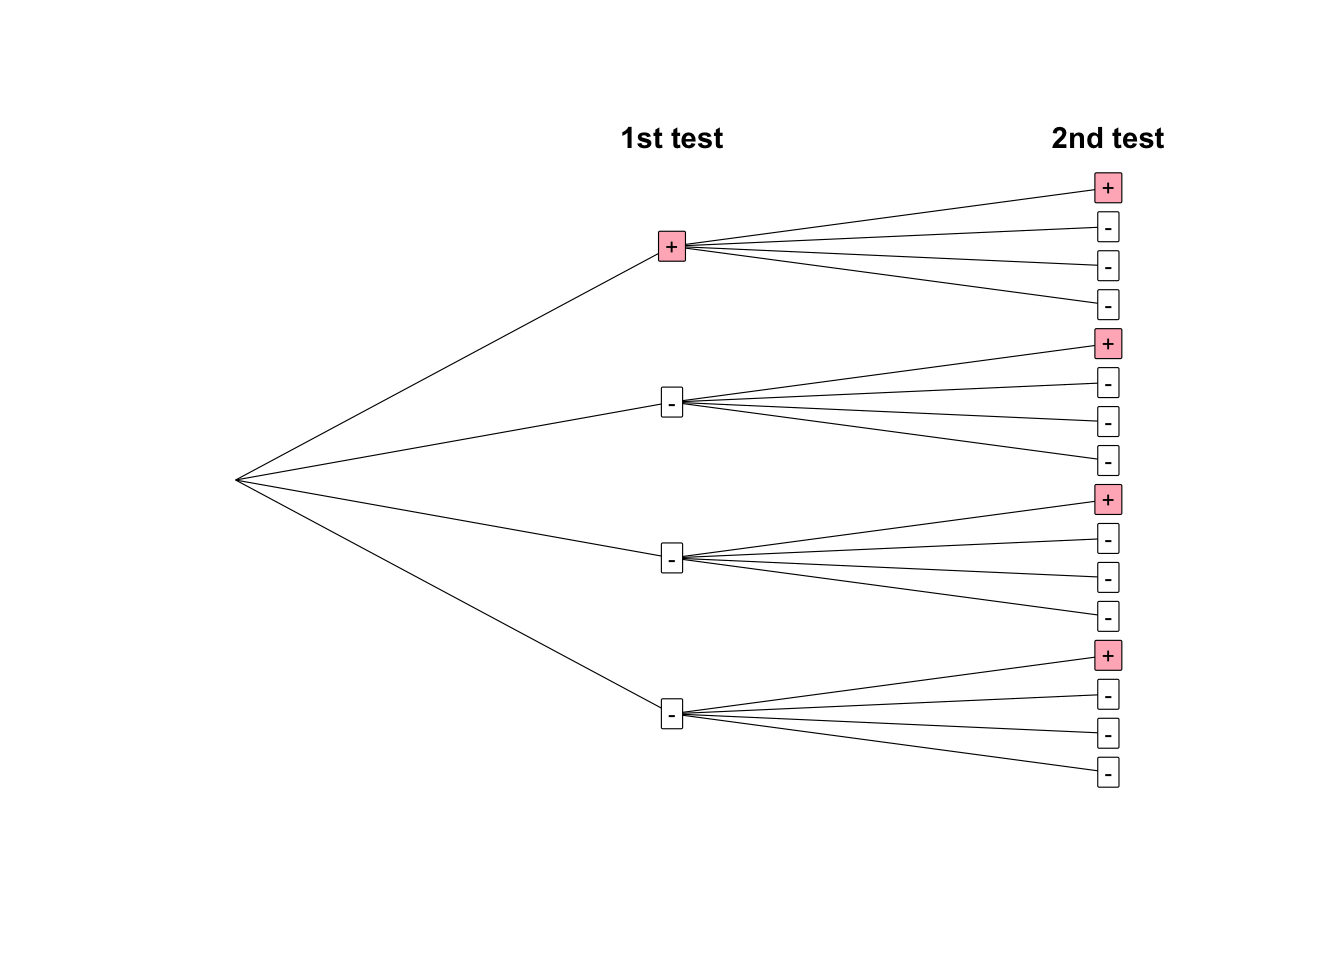
\includegraphics{Research-Design---Statistics_files/figure-latex/c7f1-1} 

}

\caption{Probability tree showing the possible outcomes of testing when one of four people in the household are infected. Pink boxes with + indicate a positive test, and white boxes with - indicate a negative test.}\label{fig:c7f1}
\end{figure}

The boxes in each branch of the tree represents the four family members. Only one of the four members is infected in this scenario, so for the 1st test, we see there's three more ways to see a negative test than a positive test. In other words, when we randomly select an individual for the first test, there's a 25\% chance of a positive test and a 75\% chance of a negative test when one of four individuals is infected. We then repeat that process for the 2nd test. Because we're sampling with replacement, the possibilities on the 2nd test are the same as the 1st test.

We can then see that when one of four family members is truly infected, there are 16 distinct outcomes when we conduct two tests. How many of those outcomes are consistent with the data we observed, that being one positive test and one negative test? There are six possible ways to get one positive test and one negative test. Those outcomes are highlighted in Figure \ref{fig:c7f2}.

\begin{figure}

{\centering 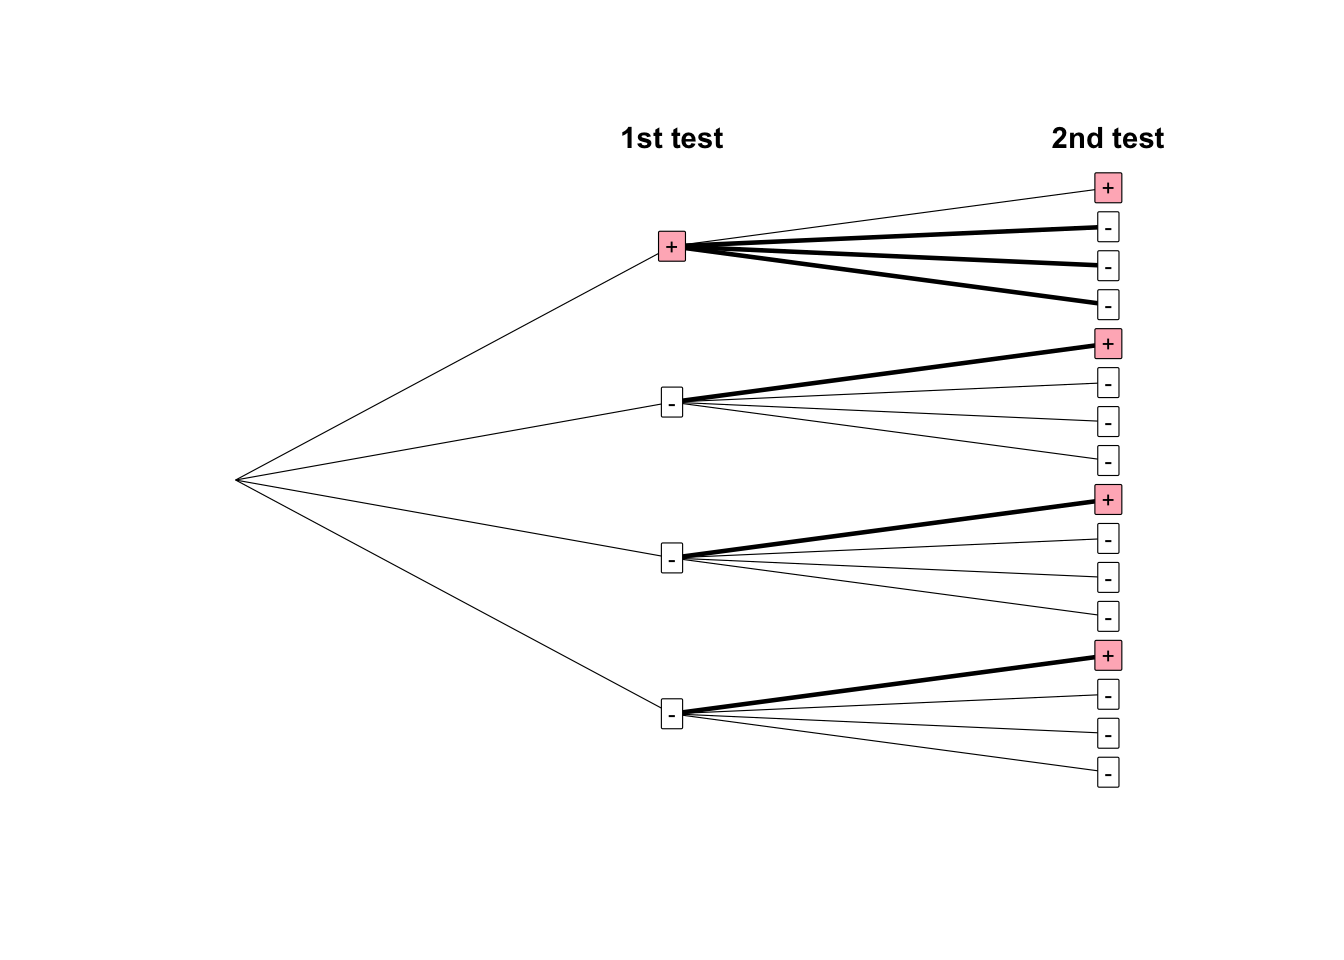
\includegraphics{Research-Design---Statistics_files/figure-latex/c7f2-1} 

}

\caption{Probability tree showing the possible outcomes of testing when one of four people in the household are infected, highlighting outcomes consistent with the observed data.}\label{fig:c7f2}
\end{figure}

Probability trees like this are really handy for looking at all the possible outcomes of joint events, but we can apply our probability rules to compute the probability of one positive out of two tests when the probability of infection is 0.25. You might be tempted to apply the multiplication rule, because we want to know the probability of a positive test \emph{and} a negative test. Applying that rule, we find \(P(+\ \text{and}\ -) = P(+)P(-) = 0.25*0.75=0.1875\). Why isn't this correct? The problem is not independence. We can reasonably assume the test results are independent if we are randomly picking one of the four people in the house for each test. The problem is that there are multiple ways of observing exactly one positive test and one negative test! You can see this in the probability tree. It could be that the first test is positive and the second test is negative (``+-''), which can happen in three ways, or it could be that the first test is negative and the second test is positive (``-+''), which can also happen in three ways. We can separately quantify \(P(+\ \text{and}\ -)\) and \(P(-\ \text{and}\ +)\), and then apply our addition rule because these outcomes are mutually exclusive.

\[
P(\text{One +}\ \text{and}\ \text{One}\ - ) = P(+)P(-) + P(-)P(+)\\
P(\text{One +}\ \text{and}\ \text{One}\ - ) = 0.25*0.75 + 0.75*0.25=0.375
\]
\#\#\# Discrete random variables

At this point I want to formalize some important concepts from our example of conducting two tests in a family of four. What we've just shown is that \textbf{the process of sampling from a population is probabilistic}. When one of four people is infected and we take a sample of \(n = 2\) tests, the outcome that we observe has an element of chance. The outcome \(X\) positive tests is called a \textbf{random variable}, where the term \emph{random} implies an element of chance in terms of how we observe the variable. When we conduct \(n=2\) tests, we can observe one of three mutually exclusive outcomes: X = 0 positives, X = 1 positive, or X = 2 positives. Some of these outcomes are more likely than others, just like getting 5 heads when you flip a coin 10 times is more likely than getting one heads. But there's an element of chance, which is ultimately what creates much of the uncertainty we face when we estimate a quantity.

Every random variable can be characterized by a \textbf{probability distribution}, which is simply the probability of observing each mutually exclusive outcome. Mathematically, we can define the probability that a random variable \(X\) takes on each possible value \(x\) (\(P(X = x)\)). For the random variable \(X\) = \emph{number of positives out of two tests}, the probability distribution consists of \(P(X = 0)\), \(P(X = 1)\), \(P(X = 2)\). We can quantify these probabilities in different ways. First, we could simply enumerate all of the possibilities in the sample space and count up the outcomes. This has basically been done in the probability tree above. Just count the number of ways each value of the random variable can happen, and divide by the total number of possible outcomes:

\begin{Shaded}
\begin{Highlighting}[]
\CommentTok{\#P(X = 0 positives): 9 ways}
\DecValTok{9}\SpecialCharTok{/}\DecValTok{16}
\end{Highlighting}
\end{Shaded}

\begin{verbatim}
## [1] 0.5625
\end{verbatim}

\begin{Shaded}
\begin{Highlighting}[]
\CommentTok{\#P(X = 1 positives): 6 ways}
\DecValTok{6}\SpecialCharTok{/}\DecValTok{16}
\end{Highlighting}
\end{Shaded}

\begin{verbatim}
## [1] 0.375
\end{verbatim}

\begin{Shaded}
\begin{Highlighting}[]
\CommentTok{\#P(X = 2 positives): 1 way}
\DecValTok{1}\SpecialCharTok{/}\DecValTok{16}
\end{Highlighting}
\end{Shaded}

\begin{verbatim}
## [1] 0.0625
\end{verbatim}

Second, we could apply our probability rules:

\begin{Shaded}
\begin{Highlighting}[]
\CommentTok{\#P(X = 0 positives) = P(negative and negative)}
\NormalTok{(}\FloatTok{0.75}\SpecialCharTok{*}\FloatTok{0.75}\NormalTok{)}
\end{Highlighting}
\end{Shaded}

\begin{verbatim}
## [1] 0.5625
\end{verbatim}

\begin{Shaded}
\begin{Highlighting}[]
\CommentTok{\#P(X = 1 positives) = P(positive and negative)}
\NormalTok{(}\FloatTok{0.75}\SpecialCharTok{*}\FloatTok{0.25}\NormalTok{) }\SpecialCharTok{+}\NormalTok{ (}\FloatTok{0.25}\SpecialCharTok{*}\FloatTok{0.75}\NormalTok{) }\CommentTok{\#2 ways this can happen}
\end{Highlighting}
\end{Shaded}

\begin{verbatim}
## [1] 0.375
\end{verbatim}

\begin{Shaded}
\begin{Highlighting}[]
\CommentTok{\#P(X = 2 positives) = P(positive and positive)}
\NormalTok{(}\FloatTok{0.25}\SpecialCharTok{*}\FloatTok{0.25}\NormalTok{) }
\end{Highlighting}
\end{Shaded}

\begin{verbatim}
## [1] 0.0625
\end{verbatim}

Third, we could use R to simulate the process of conducting two tests many, many times, record the number of positives each time, and then quantify the probability of each outcome across all the simulations.

\begin{Shaded}
\begin{Highlighting}[]
\FunctionTok{set.seed}\NormalTok{(}\DecValTok{123}\NormalTok{)}

\CommentTok{\#create a vector representing 25\% infected in a family of 4}
\NormalTok{infections }\OtherTok{\textless{}{-}} \FunctionTok{c}\NormalTok{(}\DecValTok{1}\NormalTok{, }\FunctionTok{rep}\NormalTok{(}\DecValTok{0}\NormalTok{, }\DecValTok{3}\NormalTok{))}

\CommentTok{\#create an empty vector to store the number of positives across 1 million sims}
\NormalTok{x }\OtherTok{\textless{}{-}} \FunctionTok{rep}\NormalTok{(}\ConstantTok{NA}\NormalTok{, }\DecValTok{1000000}\NormalTok{)}

\CommentTok{\#simulate 2 tests 1 million times \& record \# positives each time}
\ControlFlowTok{for}\NormalTok{(i }\ControlFlowTok{in} \DecValTok{1}\SpecialCharTok{:}\FunctionTok{length}\NormalTok{(x)) \{}
\NormalTok{  x.trial }\OtherTok{\textless{}{-}} \FunctionTok{sample}\NormalTok{(infections, }\DecValTok{2}\NormalTok{, }\AttributeTok{replace=}\ConstantTok{TRUE}\NormalTok{)}
\NormalTok{  x[i] }\OtherTok{\textless{}{-}} \FunctionTok{sum}\NormalTok{(x.trial)}
\NormalTok{\}}

\CommentTok{\#quantify the probability of each outcome}
\FunctionTok{prop.table}\NormalTok{(}\FunctionTok{table}\NormalTok{(x))}
\end{Highlighting}
\end{Shaded}

\begin{verbatim}
## x
##        0        1        2 
## 0.561914 0.375773 0.062313
\end{verbatim}

Let's walk through this code. First, the vector \texttt{infections} is created to represent the infection status of each member of the family, where a \texttt{1} represents an infected individual, and \texttt{0} represents uninfected individuals. Next, a vector \texttt{x} is created to store the results of the simulations. The vector is initiated with all NA values. Third, the simulation is conducted with a \texttt{for} loop. A \texttt{for} loop is a programming approach to execute a block of code repeatedly for a specified number of times. The total number of simulations should be the length of the \texttt{x} vector for the output, which is 1 million. The loop executes the code each each time, where \texttt{i} is the particular iteration (1 to 1,000,000). In each iteration, the \texttt{sample} function is used to randomly sample two observations from infections with replacement (\texttt{replace=TRUE}), which returns a vector \texttt{x.trial} of the observations (\{0,0\}, \{0,1\}, \{1,0\}, or \{1,1\}). We then sum the values of \texttt{x.trial}, which represents the number of positives, and store that value in \texttt{x}. Finally, the \texttt{prop.table} and \texttt{table} functions are used to compute the probability of each outcome. Lo and behold, we see largely the same quantities of probability for each value of \texttt{x} as we saw before. These aren't exact probabilities because they are based on a finite number of simulations (another great illustration of how we can't escape uncertainty when sampling).

The probabilities for each possible of outcome, no matter how we quantify them, form a probability distribution. This particular example is a \textbf{discrete probability distribution} because the sample space is composed of discrete, mutually exclusive outcomes where we can quantify the probability of each as we have done. Figure \ref{fig:c7f3} shows the probability distribution.

\begin{figure}

{\centering 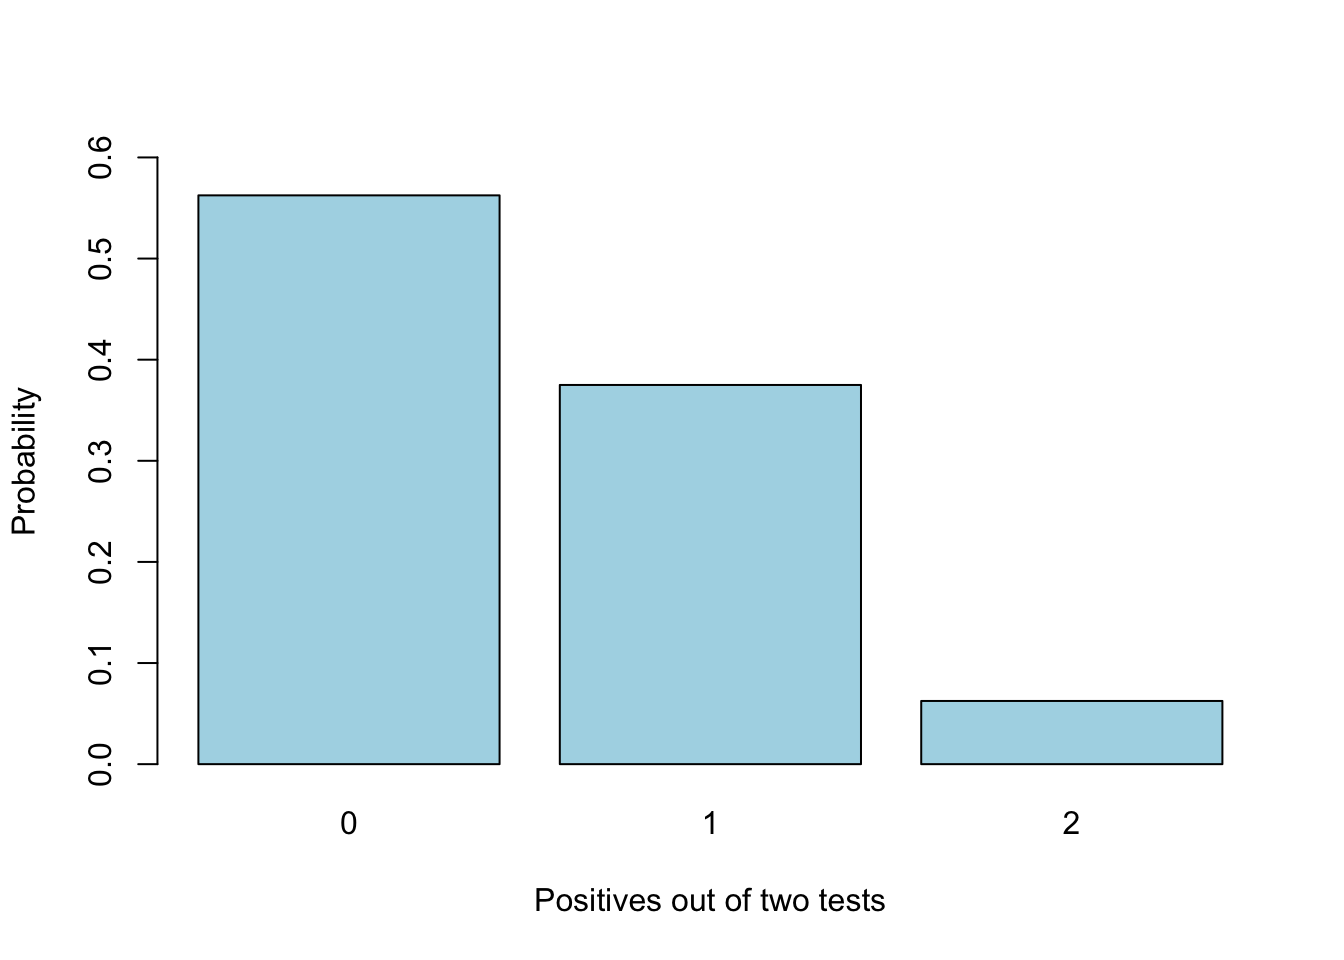
\includegraphics{Research-Design---Statistics_files/figure-latex/c7f3-1} 

}

\caption{Discrete probability distribution of the number of positive tests out of two trials.}\label{fig:c7f3}
\end{figure}

The probability of discrete outcomes is referred to as \textbf{probability mass}, but as Figure \ref{fig:c7f3} shows, the y-axis of discrete probability distributions will often just be labeled ``probability''.

\subsubsection{Binomial distribution}\label{binomial-distribution}

It was pretty straightforward to quantify the probability distribution for the number of positives out of only two tests. The sample space is so small that we could easily quantify those probabilities by applying our probability rules. But what if we randomly conduct 10 tests, or 100 tests, or 1000 tests from the broader community of 10,000? Manually enumerating the probability distribution for each possible number of positives would take considerable time! Fortunately we don't have to do that.

The random variable that we defined - the number of positives \emph{X} out of \emph{n} trials - is actually an example of a variable that follows a known mathematical function called the \textbf{binomial distribution}. A binomial distribution is a probability distribution for a binary variable where the outcome of that binary variable is examined across \emph{n} trials {[}\^{}ch07-2{]}. The sample space of each trial must be binary, for example heads and tails when flipping a coin, even or odd when rolling a die, and positive or negative when testing for a viral infection. The outcome being recorded is often generically referred to as a \textbf{success}. The \emph{n} trials must be independent and have the same probability of success, \emph{p}, which is the only parameter for the binomial distribution (e.g., probability of positive test). If those assumptions are met, the probability of \emph{x} successes out of \emph{n} trials can be computed with the binomial formula:

\[
P(X = x) = \binom{n}{x} p^x (1 - p)^{n - x}
\]
{[}\^{}ch07-2{]}: Each individual trial of a binomial process is called a \textbf{Bernoulli trial}. The \(binom{n}{x}\) part of the formula reads ``n choose x'' and represents the number of ways \emph{x} successes can occur out of \emph{n} trials without regard to order (i.e., \textbf{combinations}). For example, we've already seen that 1 positive test can occur in two ways based on 2 trials. The number of combinations can be quantified as

\[
\binom{n}{x} = \frac{n!}{x!(n-x)!}
\]
Suppose I randomly sample 10 people from the community of 10,000 where the prevlaence of infection is 0.05. What's the probability of observing exactly two infections? Just apply the binomial formula:

\[
P(X = 2) = \binom{10}{2} 0.05^2 (1 - 0.05)^{10 - 2}=0.075
\]
I'm not going to go into details here, but if you work through this formula, you'll see that all it's doing is applying the multiplication rule for independent events and the addition rule for mutually exclusive outcomes. And fortunately for us, we don't have to do these calculations by hand because R has a built-in function to compute the binomial probability: \texttt{dbinom}. For example, we can use the function to quantify the probability of 2 infections out of 10 trials:

\begin{Shaded}
\begin{Highlighting}[]
\FunctionTok{dbinom}\NormalTok{(}\AttributeTok{x =} \DecValTok{2}\NormalTok{, }\AttributeTok{size =} \DecValTok{10}\NormalTok{, }\AttributeTok{prob =} \FloatTok{0.05}\NormalTok{)}
\end{Highlighting}
\end{Shaded}

\begin{verbatim}
## [1] 0.0746348
\end{verbatim}

We can apply the \texttt{dbinom} formula to efficiently compute the binomial probability of all possible values of X positive tests out of 10 trials, when the probability of infection is 0.05, and then display the probability distribution in a graph (Figure \ref{fig:c7f4}):

\begin{figure}

{\centering 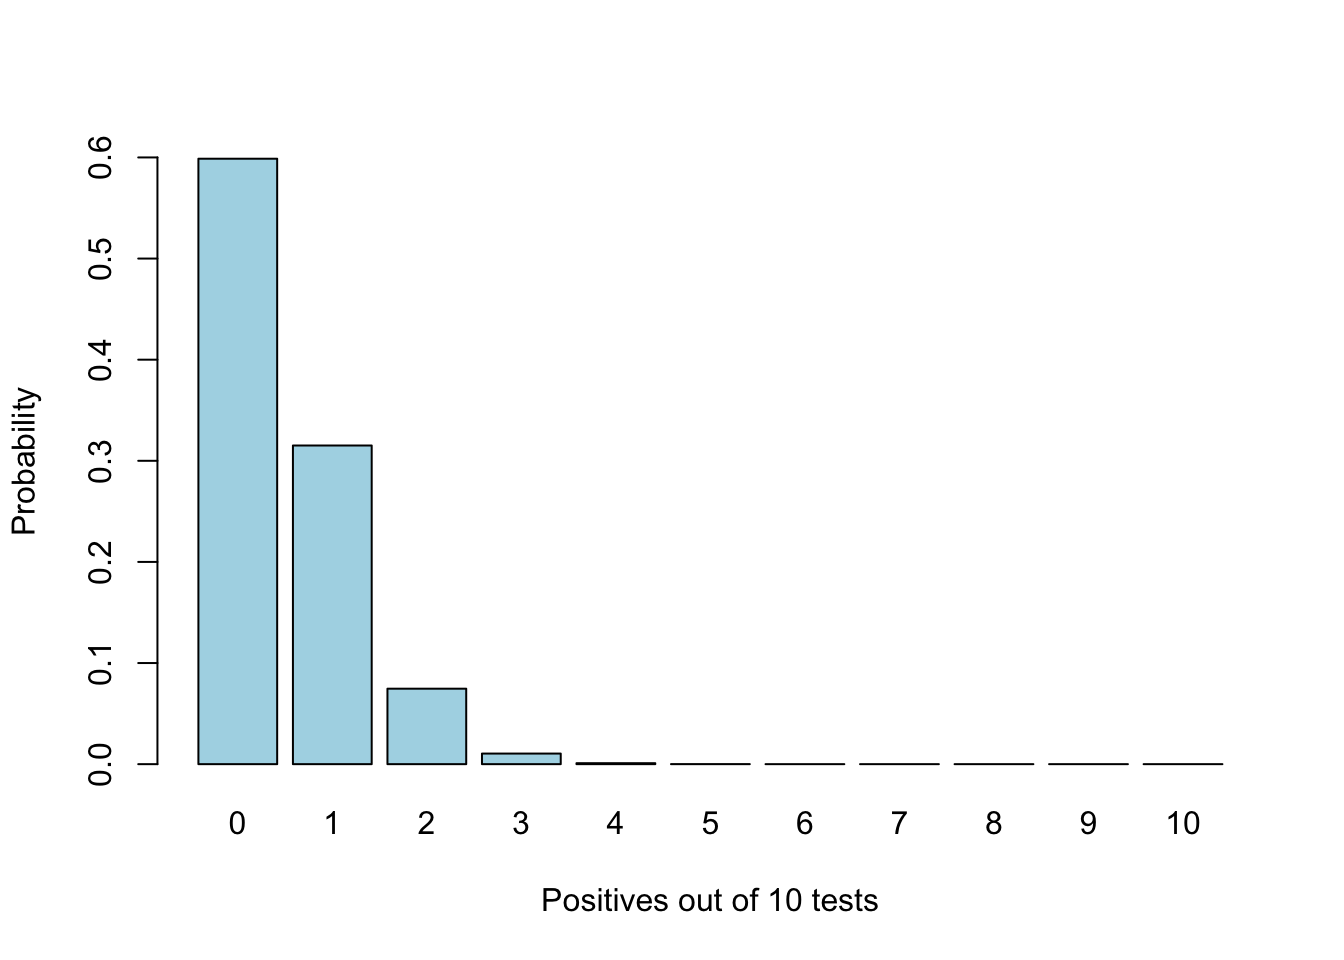
\includegraphics{Research-Design---Statistics_files/figure-latex/c7f4-1} 

}

\caption{Discrete probability distribution of the number of positive tests out of 10 trials when 5\% of the population is infected.}\label{fig:c7f4}
\end{figure}

The probability distribution shows that the most likely outcome is no positives out of 10 when the prevalence is 0.05, and the probability of each outcome decreases as the number of positives increases. That shouldn't be too surprising given that only 5\% of the population is infected. The probability distribution would look much different if 50\% of the population was infected (Figure \ref{fig:c7f5}).

\begin{figure}

{\centering 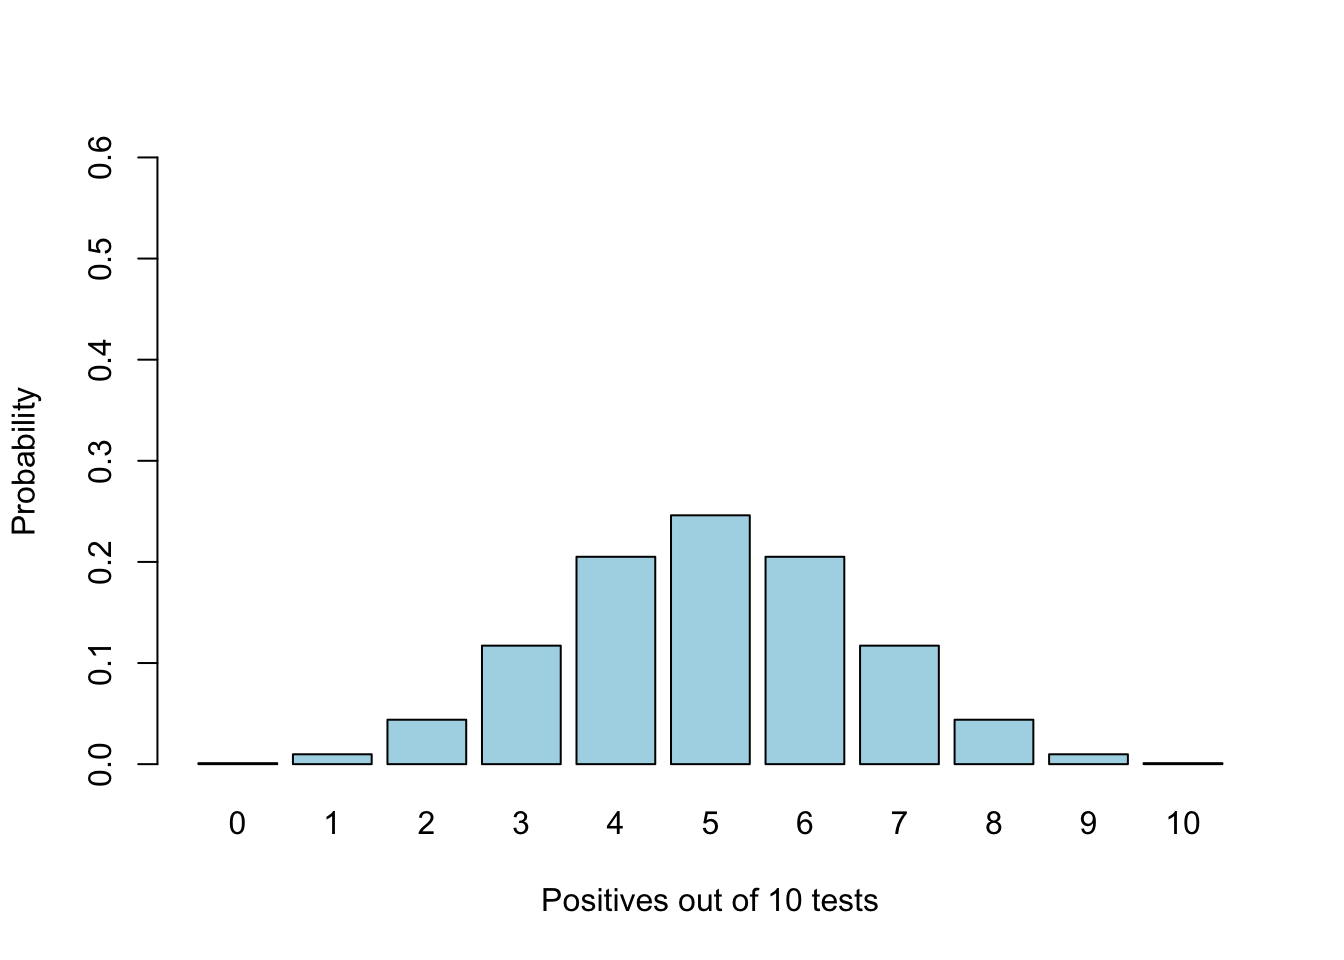
\includegraphics{Research-Design---Statistics_files/figure-latex/c7f5-1} 

}

\caption{Discrete probability distribution of the number of positive tests out of 10 trials when 50\% of the population is infected.}\label{fig:c7f5}
\end{figure}

When 50\% of the population is infected, the most likely outcome is 5 positive tests out of 10, but other values are distinctly possible due to sampling error. In fact, it's more likely than not to get a value other than 5 positives. Let's apply our \emph{not rule} to see the exact probability:

\begin{Shaded}
\begin{Highlighting}[]
\DecValTok{1} \SpecialCharTok{{-}} \FunctionTok{dbinom}\NormalTok{(}\DecValTok{5}\NormalTok{, }\DecValTok{10}\NormalTok{, }\AttributeTok{prob=}\FloatTok{0.5}\NormalTok{)}
\end{Highlighting}
\end{Shaded}

\begin{verbatim}
## [1] 0.7539062
\end{verbatim}

Here we see there's a 75\% chance of observing a value other than 5 positive tests out of 10 when the prevalence of the disease is 50\%. This is an excellent illustration of the problem of sampling error, the same sampling error that you'd expect when flipping a coin 10 times.

\paragraph{Mean for a binomial random variable}\label{mean-for-a-binomial-random-variable}

As we saw in Chapter 2, we can characterize the shape of distributions by their central tendency and variation. When examining probability distributions of random variables, central tendency is usually characterized by the mean, also known as the \textbf{expected value}. The expected value of each possible outcome \emph{X} is

\[
E[X] = \sum_{X}P(X)X
\]

Expected value is simply weighing each possible outcome of the random variable \emph{X} by its probability of occurring. Let's quantify the expected value of the number of positives out of 10 tests when the prevalence is 50\%:

\begin{Shaded}
\begin{Highlighting}[]
\CommentTok{\#create a vector of outcomes}
\NormalTok{x }\OtherTok{\textless{}{-}} \FunctionTok{c}\NormalTok{(}\DecValTok{0}\SpecialCharTok{:}\DecValTok{10}\NormalTok{)}

\CommentTok{\#sum the products of each outcome and its probability}
\FunctionTok{sum}\NormalTok{(}\FunctionTok{dbinom}\NormalTok{(}\AttributeTok{x=}\NormalTok{x, }\AttributeTok{size=}\DecValTok{10}\NormalTok{, }\AttributeTok{prob=}\FloatTok{0.5}\NormalTok{)}\SpecialCharTok{*}\NormalTok{x)}
\end{Highlighting}
\end{Shaded}

\begin{verbatim}
## [1] 5
\end{verbatim}

We see exactly what we expect. When the prevalence is 50\% and we conduct 10 tests, we expect 5 positives on average. What if the prevalence was 5\%?

\begin{Shaded}
\begin{Highlighting}[]
\FunctionTok{sum}\NormalTok{(}\FunctionTok{dbinom}\NormalTok{(}\AttributeTok{x=}\NormalTok{x, }\AttributeTok{size=}\DecValTok{10}\NormalTok{, }\AttributeTok{prob=}\FloatTok{0.05}\NormalTok{)}\SpecialCharTok{*}\NormalTok{x)}
\end{Highlighting}
\end{Shaded}

\begin{verbatim}
## [1] 0.5
\end{verbatim}

When the prevalence is 5\%, we expect 0.5 positives on average. Obviously you can't observe 0.5 positives for a discrete random variable, so you need to think about the expected value of discrete random variables as the long run outcome. That is, if you could take thousands of samples of 10 and compute the mean of the number of positives across samples, you'd expect the mean to be 0.5 positives. Remember that we can actually do that via simulation in R:

\begin{Shaded}
\begin{Highlighting}[]
\FunctionTok{set.seed}\NormalTok{(}\DecValTok{123}\NormalTok{)}

\CommentTok{\#create a vector representing 5\% infected in a population of 100}
\NormalTok{infections }\OtherTok{\textless{}{-}} \FunctionTok{c}\NormalTok{(}\FunctionTok{rep}\NormalTok{(}\DecValTok{1}\NormalTok{, }\DecValTok{5}\NormalTok{), }\FunctionTok{rep}\NormalTok{(}\DecValTok{0}\NormalTok{, }\DecValTok{95}\NormalTok{))}

\CommentTok{\#create an empty vector to store the number of positives across 1 million sims}
\NormalTok{x }\OtherTok{\textless{}{-}} \FunctionTok{rep}\NormalTok{(}\ConstantTok{NA}\NormalTok{, }\DecValTok{1000000}\NormalTok{)}

\CommentTok{\#simulate 10 tests 1 million times \& record \# positives each time}
\ControlFlowTok{for}\NormalTok{(i }\ControlFlowTok{in} \DecValTok{1}\SpecialCharTok{:}\FunctionTok{length}\NormalTok{(x)) \{}
\NormalTok{  x.trial }\OtherTok{\textless{}{-}} \FunctionTok{sample}\NormalTok{(infections, }\DecValTok{10}\NormalTok{, }\AttributeTok{replace=}\ConstantTok{TRUE}\NormalTok{)}
\NormalTok{  x[i] }\OtherTok{\textless{}{-}} \FunctionTok{sum}\NormalTok{(x.trial)}
\NormalTok{\}}

\CommentTok{\#quantify the expected value}
\FunctionTok{mean}\NormalTok{(x)}
\end{Highlighting}
\end{Shaded}

\begin{verbatim}
## [1] 0.500318
\end{verbatim}

The simulation shows that we expect 0.500351 positive tests out of 10, almost exactly the correct answer.

For binomial random variables, the mean of the probability distribution is equal to the true probability of success, so the expected value of a binomial random variable can be quantified simply as \(E(X) = np\), where \(n\) is the number of trials and \(p\) is the probability of success. For example, when we take \(n = 10\) tests from a population with \(p_{infection} = 0.05\), the expected value can be computed as \(E(X) = np=10*0.05=0.5\).

\paragraph{Variance for a binomial random variable}\label{variance-for-a-binomial-random-variable}

Recall that variance is a measure of variation in an outcome relative to the mean. The variance will be large when outcomes of the random variable can range widely around the mean, and it will be small when the outcomes show little variation around the mean. For a binomial random variable, the variance is quantified as

\[
V[X]=\sum_{X}P(X)(X-E[X])^2
\]
What does this mean? Just like we saw in the variance formula before, we're looking at how far each value of X is away from the mean, quantified as the squared difference between \(X\) and \(E[X]\). We weigh each of those squared deviations by the probability of X, \(P(X)\), and then we sum them up. Intuitively, you should see that the variance will increase as there are highly probable values of \(X\) far from the mean.

The variance formula for a binomial random variable can be simplified to the following:

\[
V[X]=p(1-p)
\]
From this formula we can see that the variance of a binomial random variable will be greatest when the probability of success is closer to 0.5. When \(p=0.5\), the variance is \(V[X]=0.5(1-0.5)=0.25\). Any deviation from \(p = 0.5\) leads to lower variance. For example, when \(p=0.05\) (e.g., 5\% prevalence of infection), the variance is \(V[X]=0.05(1-0.05)=0.0475\). At the extremes, when \(p = 0\) or \(p = 1\), the variance by definition must be 0. What this means is that probability distribution for binomial random variables will be somewhat bell-shaped with long tails when the probability of success is close to 0.5, and it will become skewed as the probability distribution deviates from 0.5.

\subsection{Continuous random variables}\label{continuous-random-variables}

Discrete probability distributions are straightforward because we can quantify the probability mass for each discrete outcome in the sample space. When we test an individual for a viral infection, the outcome is either positive or negative with probabilities \(p_{positive}\) and \(p_negative\). But not all random variables are so simple. Many variables form \textbf{continuous} probability distributions, such as height, weight, air temperature, and many more. The challenge of characterizing probability distributions for continuous variables is that there's an \emph{infinite} number of potential outcomes in the sample space.

Consider the incubation period for a viral illness, which is the time between exposure to the pathogen and onset of symptoms. Incubation period is a continuous random variable because there's an infinite number of possibilities in the sample space. The incubation might be 2, 2.1, 2.15, 2.154, 2.1547 days, and so on. The probability of the incubation period being a particular value (e.g., 2.154794667 days) is 0 because there's an infinite number of possible values. If there's an infinite number of possible values in the sample space and each possibility had a non-zero probability, then the sum of the probability of all the mutually exclusive outcomes would be infinity, violating our rules of probability.

\subsubsection{Probability density function}\label{probability-density-function}

To characterize probability distributions for continuous variables, we use the concept of \textbf{probability density}. A \textbf{probability density function (pdf)} describes how probability is distributed across the possible values of a continuous random variable. Instead of assigning probabilities to individual points, the pdf reflects how ``dense'' the probability is at different values of the random variable.

To visualize this concept, we can approximate a continuous variable by discretizing the sample space into intervals. Figure \ref{fig:c7f6} shows a simulated distribution of incubation times for 10,000 individuals, grouped into bins of 0.1 days. The highlighted bin for 2.4--2.5 days contains 1,375 observations, meaning the probability mass for this interval is:

\[
\frac{1375}{10000}=0.1375
\]
The probability density is defined as the ratio of the probability mass to the bin width, in this case:

\[
\frac{0.1375}{0.1}=1.375
\]

Here we see that probability densities can be greater than 1. That's because probability density is a measure of how concentrated the probability is within a particular interval (a density!) rather than a probability of a particular observation. In this way probability density is similar to measuring human population density in a city. A city can have densities well over one person per square kilometer, even though the probability of finding one person in a randomly selected square kilometer is very low.

\begin{figure}

{\centering 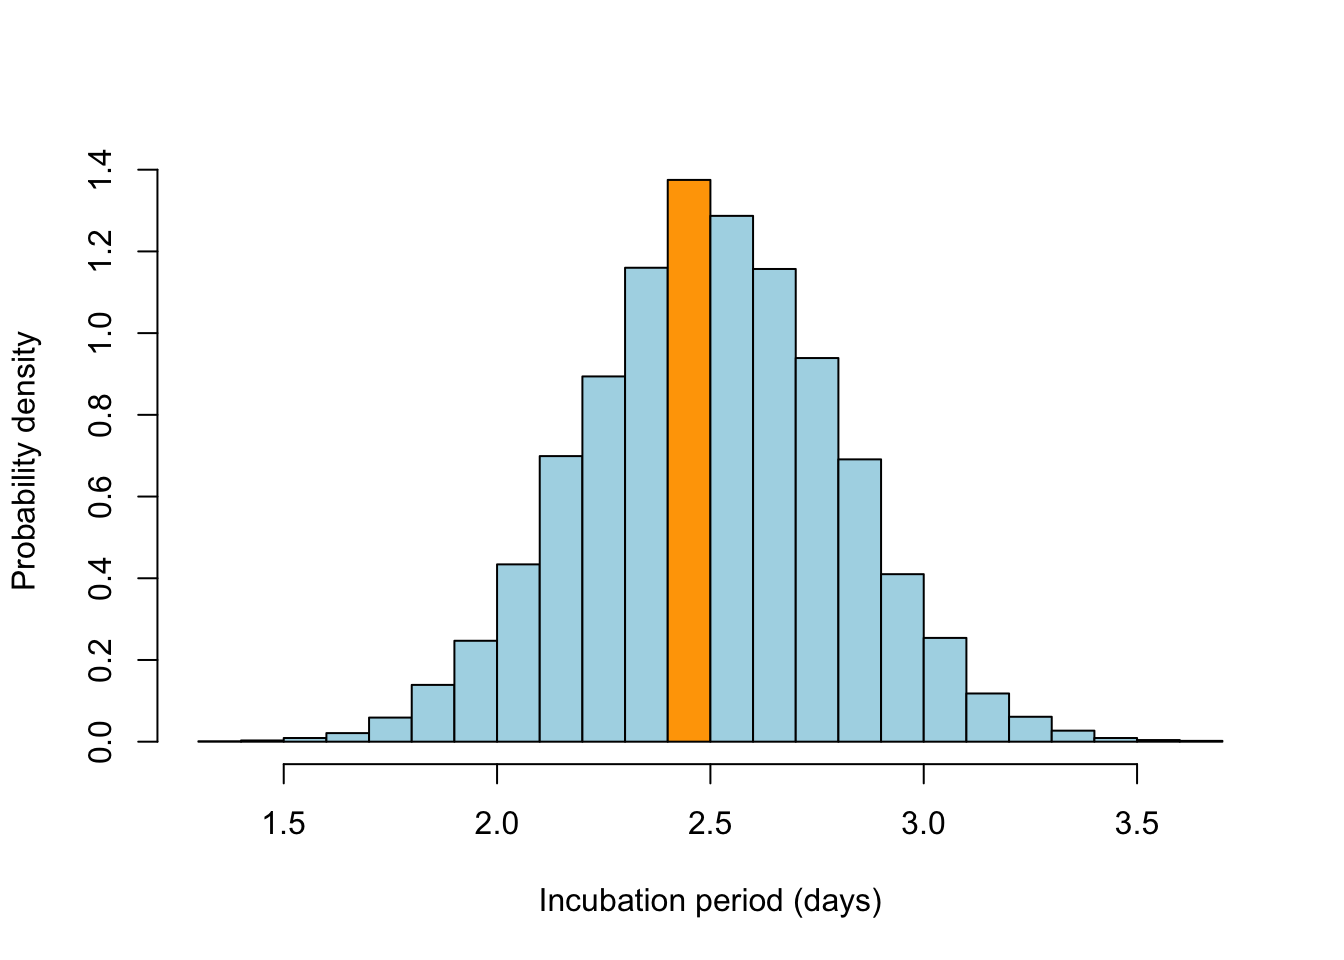
\includegraphics{Research-Design---Statistics_files/figure-latex/c7f6-1} 

}

\caption{Probability distribution of incubation period with intervals of 0.1 days.}\label{fig:c7f6}
\end{figure}

If we can quantify probability mass for a discrete interval, why do we use probability density? We use probability density because we want to describe the distribution continuously, without being constrained by arbitrary interval sizes. Narrower intervals result in smaller probability masses, approaching zero as the interval size approaches zero. The pdf allows us to describe the relative likelihood of observations without relying on a fixed bin size. Given a pdf, we can quantify the probability mass of \emph{any} interval by applying integrals from calculus, which represents the area under the curve of the pdf over the interval of interest. The total probability over the entire sample space remains one, satisfying the basic rules of probability.

\subsubsection{Normal distribution}\label{normal-distribution}

Perhaps the most well-known probability density function for a continuous random variable is the \textbf{normal distribution}, also known as a \textbf{Gaussian distribution}. The normal distribution can be used to describe any continuous variable with positive or negative values. The normal distribution is among the most recognized because many continuous variable follow a normal distribution. As we'll see, the normal distribution also tends to be important for some methods of statistical hypothesis testing.

For a normal random variable, the probability density of any value X is quantified as

\[
f(X) = \frac{1}{\sqrt{2\pi\sigma^2}} e^{-\frac{(x - \mu)^2}{2\sigma^2}}
\]
where \(f(X)\) is the probabilty density of value \(X\), \(\mu\) is the mean and \(\sigma^2\) is the variance of the random variable. This is an ugly equation, but don't fret. The main takeaway here is that a normal distribution has two parameters. The mean (\(\mu\)) controls location, and the variance (\(\sigma^2\), or standard deviation, \(\sigma\)) controls the variation or width of the normal distribution.

In R we can use the \texttt{dnorm} function to compute the probability density of \(X\) given values for \(\mu\) and \(\sigma\). For example, let's compute probability density for values between 1 and 4 days assuming incubation period follows a normal distribution with \(\mu\) = 2.5 and \(\sigma\) = 0.3 days.

\begin{figure}

{\centering 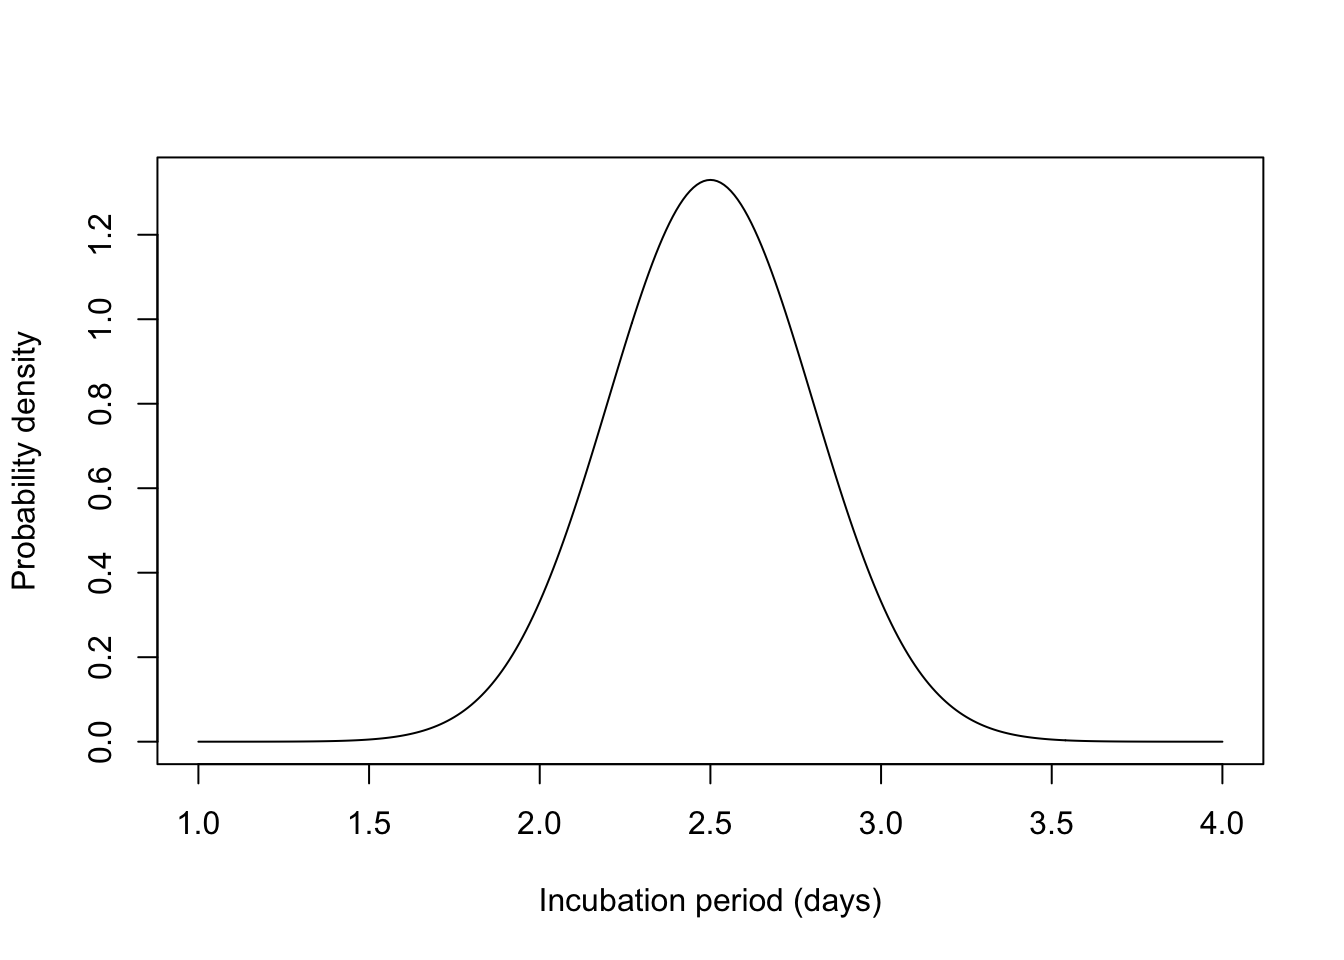
\includegraphics{Research-Design---Statistics_files/figure-latex/c7f7-1} 

}

\caption{Probability density function assuming a normal distribution of incubation period mean = 2.5 and SD = 0.3 days.}\label{fig:c7f7}
\end{figure}

Figure \ref{fig:c7f7} shows the resulting probability density function, which we can use to highlight important characteristics of the normal distribution:

\begin{enumerate}
\def\labelenumi{\arabic{enumi}.}
\tightlist
\item
  The normal distribution is bell-shaped and symmetric around the mean. In other words, the probability of incubation period being less than 2.5 days is 0.5, and the probability of incubation period being more than 2.5 days is 0.5. We can very that with the \texttt{pnorm} function, which computes the probability mass of values below a defined value when the \texttt{lower.tail} argument is \texttt{TRUE}. The probability mass greater than the defined value is computed when \texttt{lower.tail\ =\ FALSE}.
\end{enumerate}

\begin{Shaded}
\begin{Highlighting}[]
\FunctionTok{pnorm}\NormalTok{(}\FloatTok{2.5}\NormalTok{, }\AttributeTok{mean =} \FloatTok{2.5}\NormalTok{, }\AttributeTok{sd =} \FloatTok{0.3}\NormalTok{, }\AttributeTok{lower.tail=}\ConstantTok{TRUE}\NormalTok{) }\CommentTok{\#P(X\textless{}2.5)}
\end{Highlighting}
\end{Shaded}

\begin{verbatim}
## [1] 0.5
\end{verbatim}

\begin{Shaded}
\begin{Highlighting}[]
\FunctionTok{pnorm}\NormalTok{(}\FloatTok{2.5}\NormalTok{, }\AttributeTok{mean =} \FloatTok{2.5}\NormalTok{, }\AttributeTok{sd =} \FloatTok{0.3}\NormalTok{, }\AttributeTok{lower.tail=}\ConstantTok{FALSE}\NormalTok{) }\CommentTok{\#P(X\textgreater{}2.5)}
\end{Highlighting}
\end{Shaded}

\begin{verbatim}
## [1] 0.5
\end{verbatim}

The \texttt{pnorm} function is applying the integral from calculus mentioned earlier, effectively quantifying probability mass for an interval as the area under the density function curve for that interval. We can quantify probability mass for any interval in this way. For example, what's the probability that incubation period is less than 2 days?

\begin{Shaded}
\begin{Highlighting}[]
\FunctionTok{pnorm}\NormalTok{(}\DecValTok{2}\NormalTok{, }\AttributeTok{mean =} \FloatTok{2.5}\NormalTok{, }\AttributeTok{sd =} \FloatTok{0.3}\NormalTok{, }\AttributeTok{lower.tail=}\ConstantTok{TRUE}\NormalTok{) }\CommentTok{\#P(X\textless{}1.5)}
\end{Highlighting}
\end{Shaded}

\begin{verbatim}
## [1] 0.04779035
\end{verbatim}

We see there's less than a 5\% chance that incubation period is less than 2 days.

\begin{enumerate}
\def\labelenumi{\arabic{enumi}.}
\setcounter{enumi}{1}
\tightlist
\item
  The mean is the expected value of the normal distribution and specifies the central tendency of the distribution. Figure \ref{fig:c7f8} shows three normal distributions each with different means. Notice the means control where the center of the distribution is located, while the width of the distribution remains the same.
\end{enumerate}

\begin{figure}

{\centering 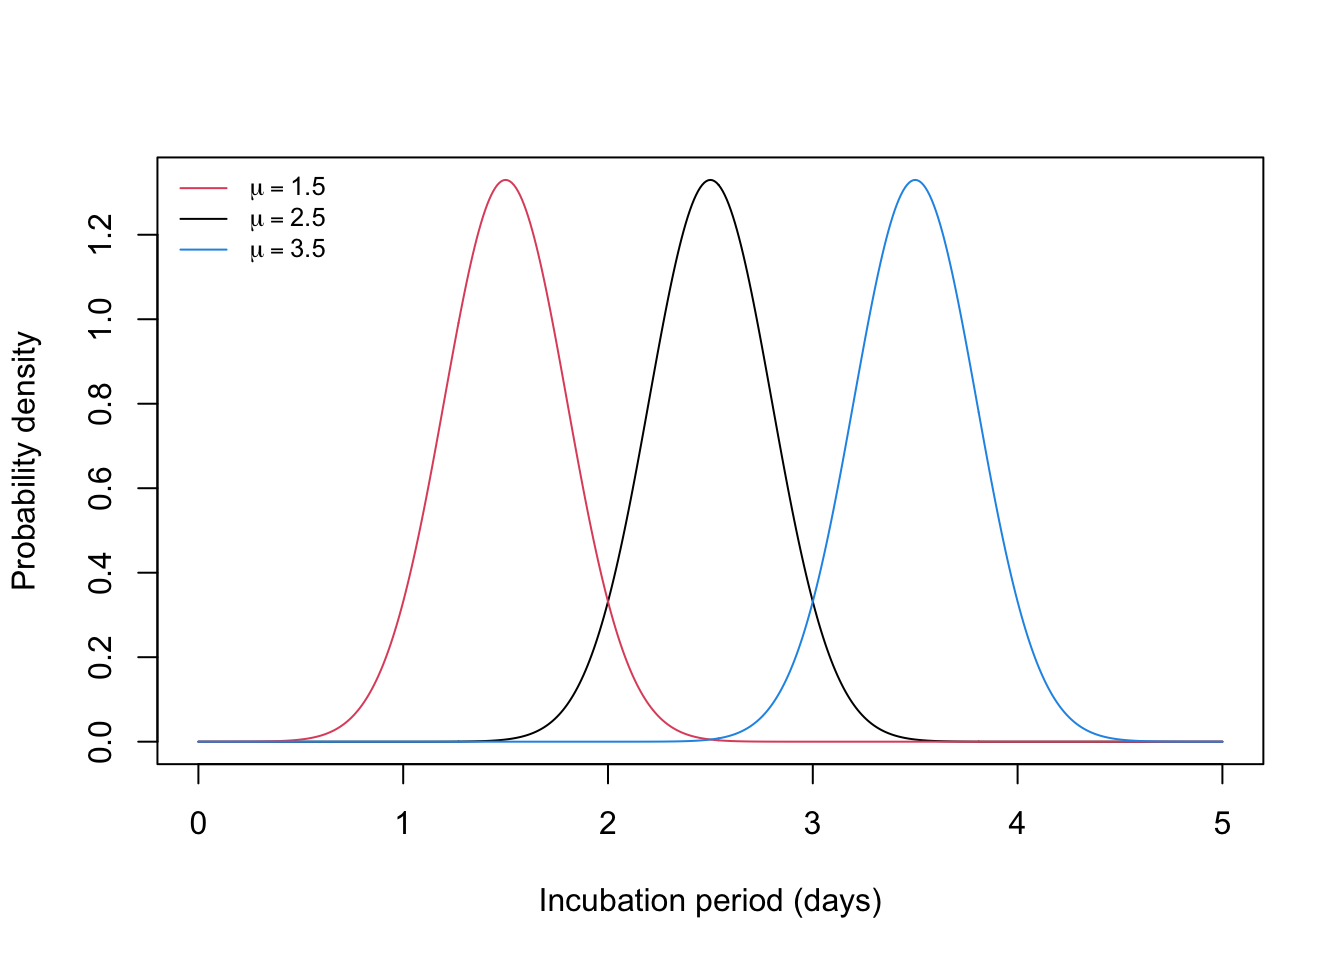
\includegraphics{Research-Design---Statistics_files/figure-latex/c7f8-1} 

}

\caption{Probability density functions with varying means but identical standard deviations.}\label{fig:c7f8}
\end{figure}

\begin{enumerate}
\def\labelenumi{\arabic{enumi}.}
\setcounter{enumi}{2}
\tightlist
\item
  The variance of a normal distribution controls the spread of the observations away from the mean, although note that unlike the binomial distribution, the variance of a normal distribution does \emph{not} depend on the value of the mean. Figure \ref{fig:c7f9} shows three normal distributions each with identical means but different standard deviations. Notice how the width of the normal distribution grows as the standard deviation increases.
\end{enumerate}

\begin{figure}

{\centering 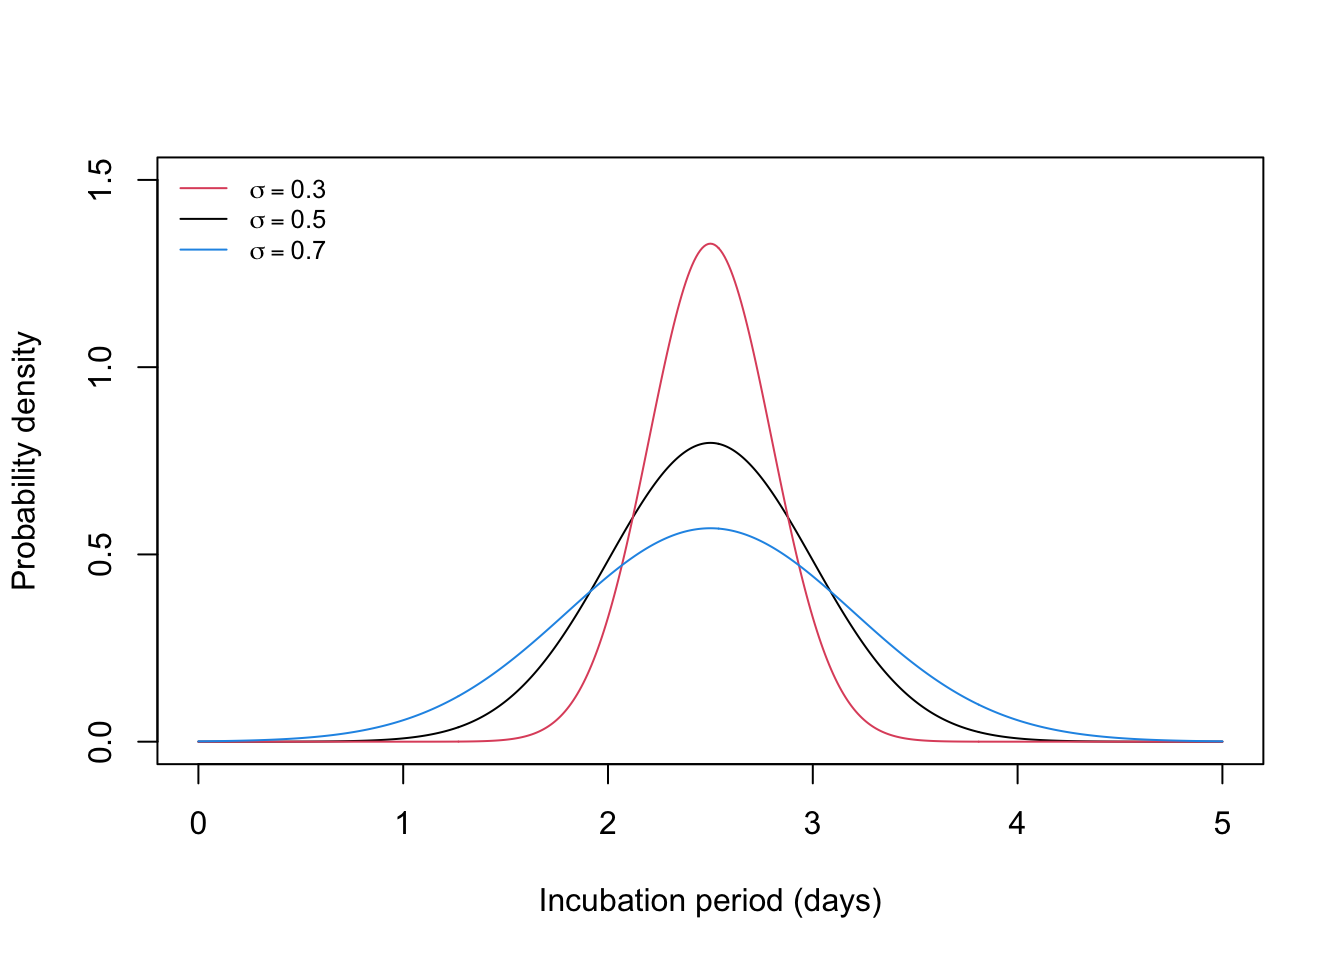
\includegraphics{Research-Design---Statistics_files/figure-latex/c7f9-1} 

}

\caption{Probability density functions with identical means but varying standard deviations.}\label{fig:c7f9}
\end{figure}

\paragraph{Probability mass and the empirical rule}\label{probability-mass-and-the-empirical-rule}

Recall that we can quantify probability mass as area under the probability density function for any interval of interest. Consider again the normal distribution with \(\mu = 2.5\) and \(\sigma = 0.3\). What's the probability that incubation period will be between 2.2 and 2.8? The interval of interest is shaded in the probability density function in Figure \ref{fig:c7f10}.

\begin{figure}

{\centering 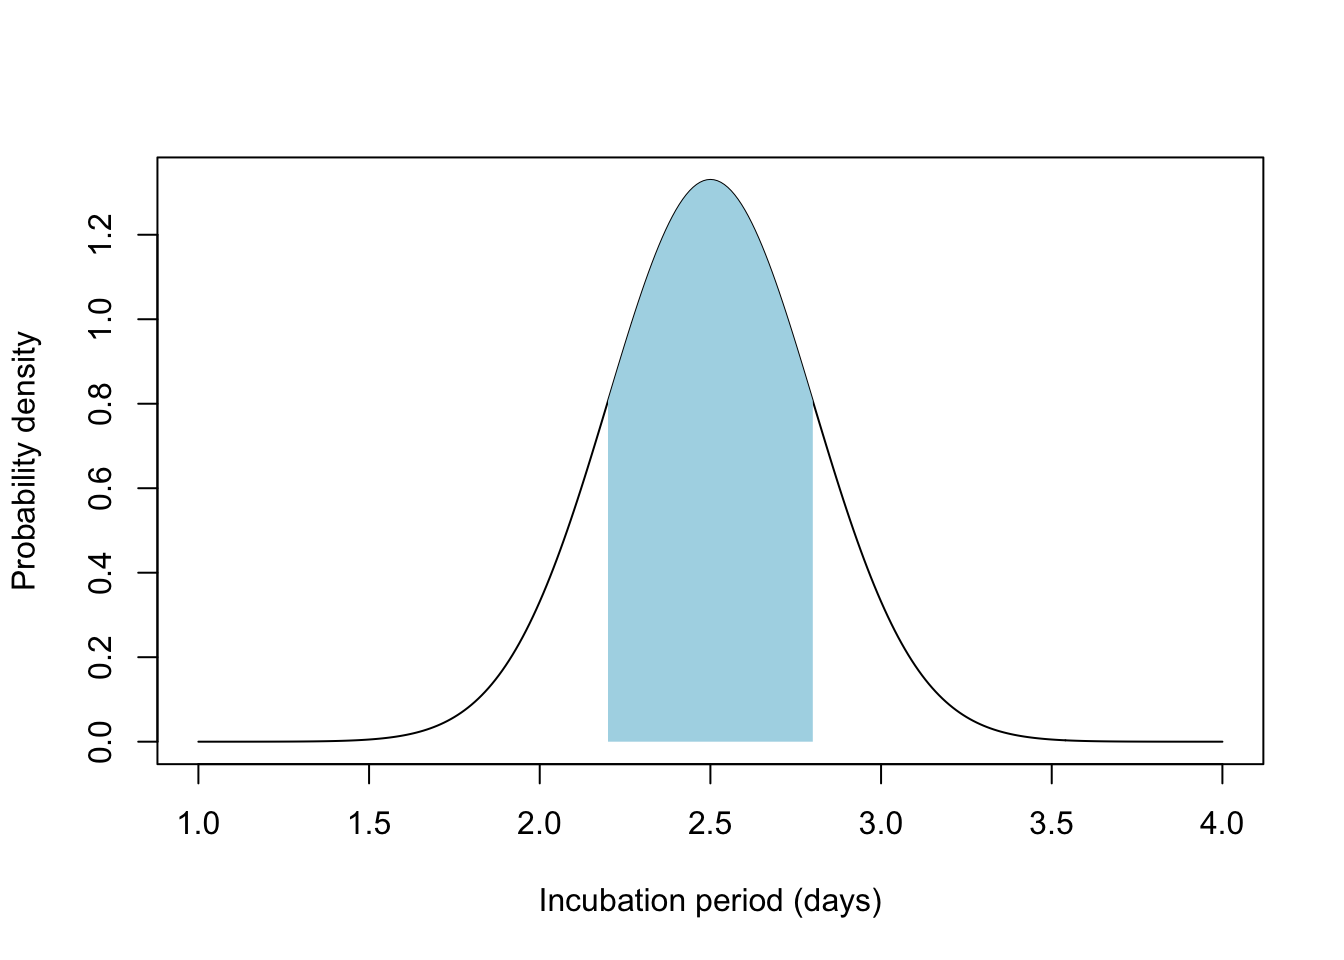
\includegraphics{Research-Design---Statistics_files/figure-latex/c7f10-1} 

}

\caption{Probability density function highlighting the interval 2.2 to 2.8}\label{fig:c7f10}
\end{figure}

We can apply the \texttt{pnorm} function to find the probability of observations between 2.2 and 2.8 as the area under the curve in that interval:

\begin{Shaded}
\begin{Highlighting}[]
\FunctionTok{pnorm}\NormalTok{(}\FloatTok{2.8}\NormalTok{, }\FloatTok{2.5}\NormalTok{, }\FloatTok{0.3}\NormalTok{, }\AttributeTok{lower.tail=}\NormalTok{T) }\SpecialCharTok{{-}} \FunctionTok{pnorm}\NormalTok{(}\FloatTok{2.2}\NormalTok{, }\FloatTok{2.5}\NormalTok{, }\FloatTok{0.3}\NormalTok{, }\AttributeTok{lower.tail=}\NormalTok{T)}
\end{Highlighting}
\end{Shaded}

\begin{verbatim}
## [1] 0.6826895
\end{verbatim}

This code asks for the probability between 2.2 and 2.8 by subtracting the cumulative probability up to 2.2 from the cumulative probability up to 2.8. We find that 68.3\% of the observations fall between 2.2 and 2.8.

How about values between 1.9 and 3.1 (Figure \ref{fig:c7f11}))?

\begin{figure}

{\centering 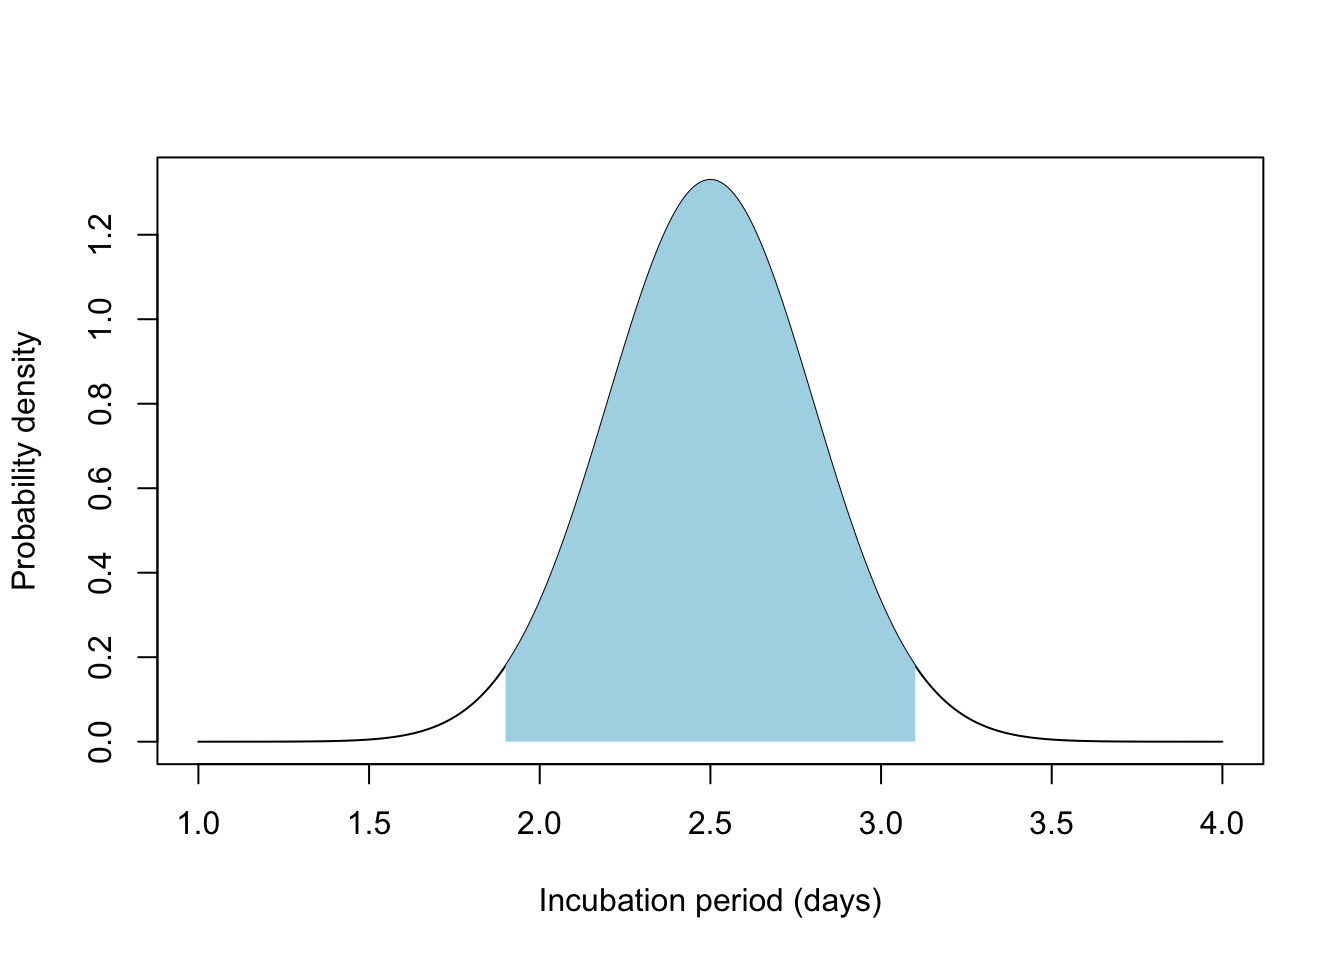
\includegraphics{Research-Design---Statistics_files/figure-latex/c7f11-1} 

}

\caption{Probability density function highlighting the interval 2.2 to 2.8}\label{fig:c7f11}
\end{figure}

\begin{Shaded}
\begin{Highlighting}[]
\FunctionTok{pnorm}\NormalTok{(}\FloatTok{1.9}\NormalTok{, }\FloatTok{2.5}\NormalTok{, }\FloatTok{0.3}\NormalTok{, }\AttributeTok{lower.tail=}\NormalTok{F) }\SpecialCharTok{{-}} \FunctionTok{pnorm}\NormalTok{(}\FloatTok{3.1}\NormalTok{, }\FloatTok{2.5}\NormalTok{, }\FloatTok{0.3}\NormalTok{, }\AttributeTok{lower.tail=}\NormalTok{F) }
\end{Highlighting}
\end{Shaded}

\begin{verbatim}
## [1] 0.9544997
\end{verbatim}

Here I quantified \(P(X>1.9)\) and subtracted \(P(X>3.1)\), which shows us that 95.4\% of values lie between 1.9 and 3.1.

It's helpful to think about probability mass as the area under the pdf and to quantify those probabilities with the \texttt{pnorm} function, but what we've also done here is illustrate the \textbf{emprical rule}. The empirical rule is that about 68\% of the probability mass falls within 1 standard deviation of the mean (i.e., \(\mu \pm 1\sigma\) ), whereas about 95\% of the probability mass falls within 2 standard deviations of the mean (i.e., \(\mu \pm 2\sigma\) ). Figure \ref{fig:c7f12} shows the empirical rule graphically for our example normal distribution of incubation period.

\begin{figure}

{\centering 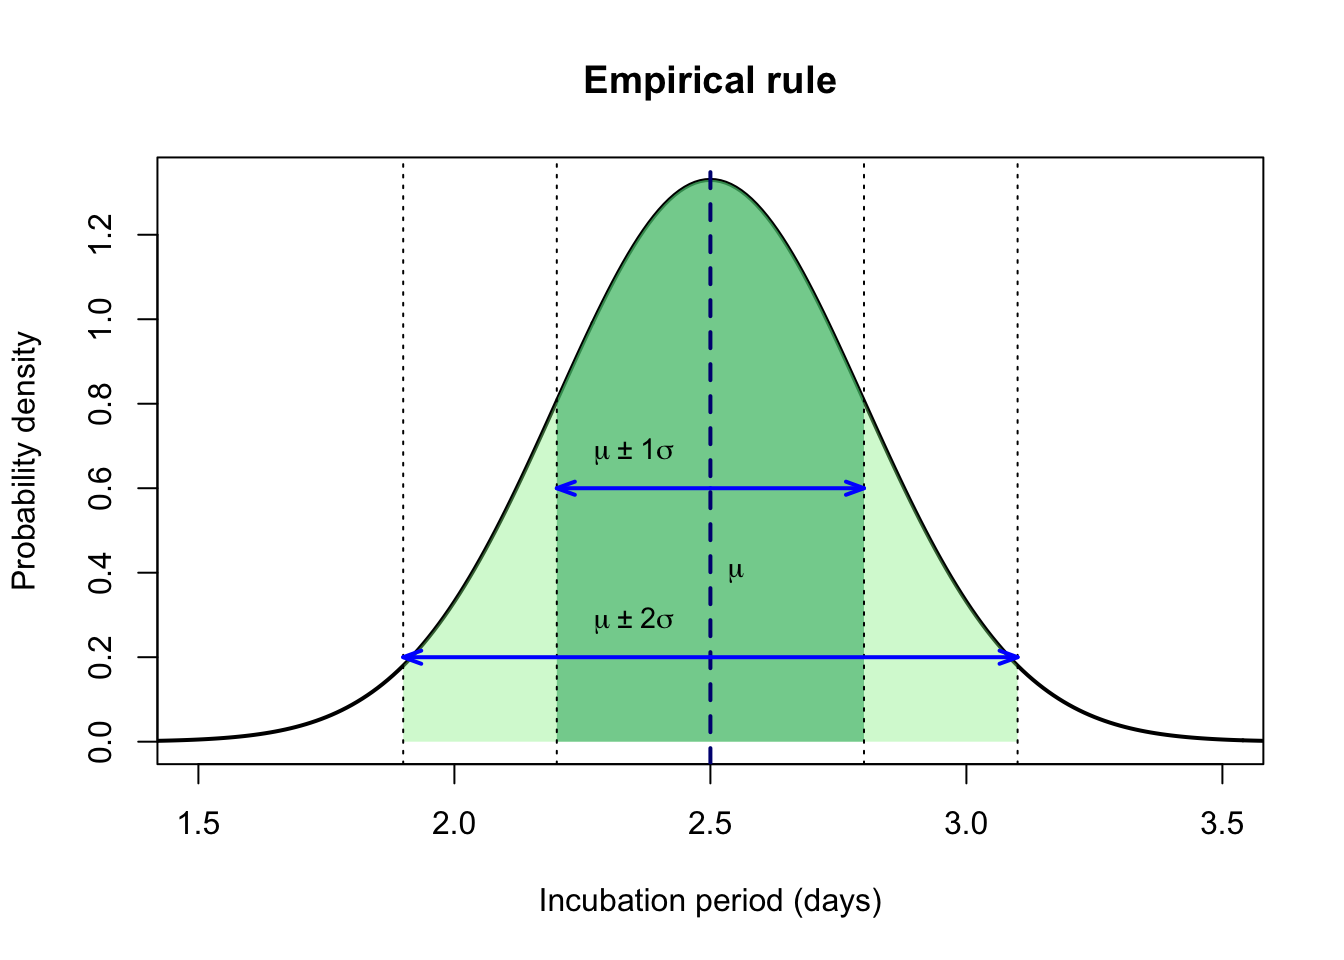
\includegraphics{Research-Design---Statistics_files/figure-latex/c7f12-1} 

}

\caption{Normal probability density function showing the empirical rule, namely that about 68\% of observations are within one standard deviation of the mean, and about 95\% of observations are within two standard deviations of the mean. In this example, the mean incubation period is 2.5 and the standard deviation is 0.3.}\label{fig:c7f12}
\end{figure}

\paragraph{Standard normal distribution}\label{standard-normal-distribution}

Any combination of \(\mu\) and \(\sigma\) produces a unique normal distribution, so there's an infinite variety of possible normal distributions. However, any normal distribution can be converted to a \textbf{standard normal distribution}, which is a normal distribution with \(\mu = 0\) and \(\sigma = 1\) (Figure \ref{fig:c7f13}). Because the standard deviation is one, the values of the standard normal distribution are in units of standard deviations. The values of a standard normal distribution are denoted \(Z\), or \(Z-scores\).

\begin{figure}

{\centering \includegraphics{Research-Design---Statistics_files/figure-latex/c7f13-1} 

}

\caption{Standard normal distribution with mean = 0 and standard deviation = 1. The values Z of a standard normal distribution are in units of standard deviations away from the mean.}\label{fig:c7f13}
\end{figure}

We can convert any observation \(X\) drawn from a normal distribution to a Z-score using the following formula:

\[
Z = \frac{X-\mu}{\sigma}
\]
Consider the normal distribution of incubation period with \(\mu = 2.5\) and \(\sigma=0.3\) days. Let's say we have an observation \(X\) of 2.8 days for the incubation period. The corresponding Z-score is thus

\[
Z = \frac{X-\mu}{\sigma} =\frac{2.8-2.5}{0.3}=1 
\]
In other words, the value 2.8 days is one standard deviation above the mean. Consider another observation \(X\) of 2.05 days:

\[
Z = \frac{X-\mu}{\sigma} =\frac{2.05-2.5}{0.3}=-1.5
\]
The negative value of \(Z\) indicates the observation \(X\) is below the mean, so can say the observation of 2.05 days is 1.5 standard deviations below the mean. The standard normal distribution is perfectly symmetric around 0, so half the observations are positive and half are negative.

The standard normal distribution is useful as a common language to talk about any normal distribution, but there's also practical value that we'll encounter in statistics of converting variables to Z-scores. The process of transforming a variable to Z-scores is called \textbf{standardization}, and in R we can use the \texttt{scale} function to make the conversion. For example, here I generate a dataset of 10 values, which I then convert to z-scores:

\begin{Shaded}
\begin{Highlighting}[]
\NormalTok{x }\OtherTok{\textless{}{-}} \FunctionTok{c}\NormalTok{(}\DecValTok{0}\NormalTok{, }\DecValTok{1}\NormalTok{, }\DecValTok{3}\NormalTok{, }\DecValTok{5}\NormalTok{, }\DecValTok{6}\NormalTok{, }\DecValTok{6}\NormalTok{, }\DecValTok{7}\NormalTok{, }\DecValTok{7}\NormalTok{, }\DecValTok{9}\NormalTok{, }\DecValTok{10}\NormalTok{)}
\NormalTok{z }\OtherTok{\textless{}{-}} \FunctionTok{scale}\NormalTok{(x)}
\NormalTok{z}
\end{Highlighting}
\end{Shaded}

\begin{verbatim}
##             [,1]
##  [1,] -1.6673586
##  [2,] -1.3585885
##  [3,] -0.7410483
##  [4,] -0.1235080
##  [5,]  0.1852621
##  [6,]  0.1852621
##  [7,]  0.4940322
##  [8,]  0.4940322
##  [9,]  1.1115724
## [10,]  1.4203425
## attr(,"scaled:center")
## [1] 5.4
## attr(,"scaled:scale")
## [1] 3.238655
\end{verbatim}

The scale function returns each value \(X\) as a Z-score, and it also computes the mean (\texttt{scaled:center}) and standard deviation (\texttt{scaled:scale}). Note that if we standardize the value directly, we'd get the same Z-scores:

\begin{Shaded}
\begin{Highlighting}[]
\NormalTok{z }\OtherTok{\textless{}{-}}\NormalTok{ (x}\SpecialCharTok{{-}}\FunctionTok{mean}\NormalTok{(x))}\SpecialCharTok{/}\FunctionTok{sd}\NormalTok{(x)}
\NormalTok{z}
\end{Highlighting}
\end{Shaded}

\begin{verbatim}
##  [1] -1.6673586 -1.3585885 -0.7410483 -0.1235080  0.1852621  0.1852621  0.4940322  0.4940322  1.1115724  1.4203425
\end{verbatim}

\subsection{Sampling from probability distributions}\label{sampling-from-probability-distributions}

Why does any of this matter?! Well, keep in mind that when we collect data to test scientific hypotheses, we're almost always sampling from a broader population. Imagine if I'm conducting a study to estimate the mean incubation period for a viral illness. I'd love to track down every single person who has the viral illness and record the incubation, but I can't do that. Instead, we rely on sampling. We know that sampling is a stochastic, or random process. In other words, the variables that we observe should be considered \emph{random} variables, and if we sample in an unbiased way, the values of the variable we observe through sampling are drawn from a probability distribution.

What probability distribution are observations of random variables drawn from? Often we don't know with certainty! We usually have to make some assumptions, ideally informed by knowledge of your particular discipline. I've introduced two broad types of probability distributions - discrete and random - and particular probability distribution of each type, the binomial (discrete) and normal (continuous) distributions. In reality, there are many more probability distributions one can choose from, and we'll encounter some others throughout the book, but the binomial and normal distributions provide a useful starting point. They may not be a perfect fit for a particular random variable (for example, a normal distribution allows for negative values, but incubation period can't be negative), but often these distributions can be useful approximations.

\subsubsection{Simulating data from probability distributions}\label{simulating-data-from-probability-distributions}

As we've seen in previous chapters and will continue to see throughout the book, it is often useful to simulate data. Simulating data requires making an assumption about a particular probability distribution from which the simulated observations are drawn. In R, we can simulate observations from probability distributions with particular functions. For example, the \texttt{rnorm} function is used to simulate data from a normal distribution. Indeed, this is exactly how I created the simulated data in the histogram for incubation period in Figur e\ref{fig:c7f6}. I assumed a normal distribution with \(\mu = 2.5\) and \(\sigma = 0.3\) and used the \texttt{rnorm} function to randomly draw 10,000 observations from that distribution:

\begin{Shaded}
\begin{Highlighting}[]
\CommentTok{\#makes the simulated data reproducible}
\FunctionTok{set.seed}\NormalTok{(}\DecValTok{123}\NormalTok{)}

\CommentTok{\#simulate 10,000 observations}
\NormalTok{x }\OtherTok{\textless{}{-}} \FunctionTok{rnorm}\NormalTok{(}\DecValTok{10000}\NormalTok{, }\AttributeTok{mean =} \FloatTok{2.5}\NormalTok{, }\AttributeTok{sd =} \FloatTok{0.3}\NormalTok{)}

\CommentTok{\#display the first 100 observations}
\NormalTok{x[}\DecValTok{1}\SpecialCharTok{:}\DecValTok{100}\NormalTok{]}
\end{Highlighting}
\end{Shaded}

\begin{verbatim}
##   [1] 2.331857 2.430947 2.967612 2.521153 2.538786 3.014519 2.638275 2.120482 2.293944 2.366301 2.867225 2.607944 2.620231 2.533205 2.333248 3.036074
##  [17] 2.649355 1.910015 2.710407 2.358163 2.179653 2.434608 2.192199 2.281333 2.312488 1.993992 2.751336 2.546012 2.158559 2.876144 2.627939 2.411479
##  [33] 2.768538 2.763440 2.746474 2.706592 2.666175 2.481426 2.408211 2.385859 2.291588 2.437625 2.120381 3.150687 2.862389 2.163067 2.379135 2.360003
##  [49] 2.733990 2.474989 2.575996 2.491436 2.487139 2.910581 2.432269 2.954941 2.035374 2.675384 2.537156 2.564782 2.613892 2.349303 2.400038 2.194427
##  [65] 2.178463 2.591059 2.634463 2.515901 2.776680 3.115025 2.352691 1.807249 2.801722 2.287240 2.293597 2.807671 2.414568 2.133785 2.554391 2.458333
##  [81] 2.501729 2.615584 2.388802 2.693313 2.433854 2.599535 2.829052 2.630554 2.402221 2.844642 2.798051 2.664519 2.571620 2.311628 2.908196 2.319922
##  [97] 3.156200 2.959783 2.429290 2.192074
\end{verbatim}

Similarly, we can use the \texttt{rbinom} function to randomly draw values from a binomial distribution. For example, let's assume infection status of individuals follows a binomial distribution with \(p_{infected} = 0.05\) (5\% of individuals infected). Here's how we can draw 10,000 observations of infection status from this distribution:

\begin{Shaded}
\begin{Highlighting}[]
\FunctionTok{set.seed}\NormalTok{(}\DecValTok{123}\NormalTok{)}

\CommentTok{\#simulate 10,000 observations}
\NormalTok{x }\OtherTok{\textless{}{-}} \FunctionTok{rbinom}\NormalTok{(}\DecValTok{10000}\NormalTok{, }\AttributeTok{size =} \DecValTok{1}\NormalTok{, }\AttributeTok{prob =} \FloatTok{0.05}\NormalTok{)}

\CommentTok{\#display the first 100 observations}
\NormalTok{x[}\DecValTok{1}\SpecialCharTok{:}\DecValTok{100}\NormalTok{]}
\end{Highlighting}
\end{Shaded}

\begin{verbatim}
##   [1] 0 0 0 0 0 0 0 0 0 0 1 0 0 0 0 0 0 0 0 1 0 0 0 1 0 0 0 0 0 0 1 0 0 0 0 0 0 0 0 0 0 0 0 0 0 0 0 0 0 0 0 0 0 0 0 0 0 0 0 0 0 0 0 0 0 0 0 0 0 0 0 0 0 0 0
##  [76] 0 0 0 0 0 0 0 0 0 0 0 1 0 0 0 0 0 0 0 0 0 0 0 0 0
\end{verbatim}

Here we see that each observation is either a 0 (not infected) or 1 (infected). The argument \texttt{size} refers to the number of trials for each observation that you're simulating, so I simulated a single trial for each observation, resulting in 10,000 values. If you simply want to simulate the total number of infections out of 10,000 people, you could do it this way:

\begin{Shaded}
\begin{Highlighting}[]
\FunctionTok{set.seed}\NormalTok{(}\DecValTok{123}\NormalTok{)}

\CommentTok{\#simulate 10,000 observations}
\NormalTok{x }\OtherTok{\textless{}{-}} \FunctionTok{rbinom}\NormalTok{(}\DecValTok{1}\NormalTok{, }\AttributeTok{size =} \DecValTok{10000}\NormalTok{, }\AttributeTok{prob =} \FloatTok{0.05}\NormalTok{)}
\NormalTok{x}
\end{Highlighting}
\end{Shaded}

\begin{verbatim}
## [1] 484
\end{verbatim}

Here we ask for one observation of 10,000 trials, and R subsequently reports 484 infections out of the 10,000 people.

\subsubsection{Statistical notation for probabilty distributions}\label{statistical-notation-for-probabilty-distributions}

Often a standard notation is used to indicate the probability distribution from which a random variable \(X\) is drawn. Usually this is done in the following format:

\[
X\sim \text{distribution name}(\text{parameters})
\]
Here X is the particular variable of interest, and ``\textasciitilde{}'' means ``is distributed as''. The name (or symbol) of the paritcular probability distribution is then indicated outside of parentheses, and the parameters for the probability distribution are recorded in the parentheses.

For example, we will indicate a random variable \(X\) follows a normal distribution by writing

\[
X\sim \text{Normal}(\mu, \sigma)
\]

which reads ``X is distributed as a normal distribution with a mean and standard deviation''). The normal distribution of incubation period would be recorded as

\[
X \sim \text{Normal}(2.5, 0.3)
\]

which reads ``The incubation period \emph{X} is distributed as a normal distribution with \(\mu = 2.5\) and \(\sigma = 0.3\)

For a binomial distribution, the notation looks like this:

\[
X\sim \text{Binomial}(n, p)
\]
where \(X\) is the number of successes of the random variable, \(n\) is the number of trials and \(p\) is the probability of success. So, a binomial distribution for infection status of 10,000 people with 5\% prevalence should be notated as

\[
X\sim \text{Binomial}(10000, 0.05)
\]
If you are drawing just a single trial for a binomial outcome, you can specify 1 for \(n\), or you can indicate the random variable has a Bernouilli distribution, which as you might recall, is simply a binomial distribution with \(n = 1\):

\[
X\sim \text{Bernoulli}(0.05)
\]

\end{document}
